% !TeX encoding = UTF-8
%% \textbf{重庆大学}通用毕业论文\LaTeXe{}模板
%%% 使用前请先阅读使用文档和用户协议,内有详细介绍。Happy Texing! :)
%% =======================================================
\documentclass%
	[type=doctor, bilinguallist=apart, 
	blindtrail, printmode=auto]{cquthesis}%
% 可用选项:
% type=[bachelor|master|doctor],      % 必选,毕业论文类型,以下项目不填时为默认
% liberalformat,                      % 可选,仅适用本科生,使用文学类论文标题格式,默认未打开
% proffesionalmaster=[true|false],    % 可选,仅适用研究生,是(true)否(false)专业硕士,默认为否
% printmode=[oneside|twoside|auto],	  % 可选,论文打印方式,默认采用auto按页数要求自动判定
% openany,|openright,                 % 可选,双面打印时每章的第一页仅右页开启,默认右页开启(openright)
% bilinguallist=[off|combined|apart], % 可选,图录表录等分别按双语题注混编(combined),分开编录(apart),默认关(off)
% blindtrail,                         % 可选,盲审模式,开启后封面姓名和致谢部分会隐藏,详情请参阅用户文档,默认关
% draft,                              % 写作期间可选,不渲染图片,关闭外围功能,加快预览速度,默认未开启

% 请在cquthesis.sty文件中定义其他会用到的宏包和自己的变量
% 这样可以防止main.tex太过臃肿。
\usepackage{cquthesis}

% 定义所有的图片文件在 figures 子目录下
\graphicspath{{figures/}}

% 定义数字圆
\usepackage{tikz}
\newcommand*\circled[1]{\tikz[baseline=(char.base)]{
            \node[shape=circle,draw,inner sep=1pt] (char) {#1};}}

%*** 写作时,使用这个命令只渲染你想查看的部分,提升工作效率,定稿时注释掉整行
%\includeonly{contents/experiment,contents/analysis,}

% 默认行间距 20 pt
\linespread{1.3}

\begin{document}

\cqusetup{
%	************	注意	************
%	* 1. \cqusetup{}中不能出现全空的行,如果需要全空行请在行首注释
%	* 2. 不需要的配置信息可以放心地坐视不理、留空、删除或注释(都不会有影响)
%	*
%	********************************
% ===================
%	论文的中英文题目
% ===================
  ctitle = {面向异构车联网的车载信息物理融合系统\\关键技术研究},
  etitle = {Research on Key Techniques for Vehicular Cyber-Physical Systems in Heterogeneous Vehicular Networks},
% ===================
% 作者部分的信息
% \secretize{}为盲审标记点,在打开盲审开关时内容会自动被替换为***输出,盲审开关默认关闭
% ===================
  cauthor = \secretize{许新操},	% 你的姓名,以下每项都以英文逗号结束
  eauthor = \secretize{Xincao~Xu},	% 姓名拼音,~代表不会断行的空格
  studentid = \secretize{},	% 仅本科生,学号
  csupervisor = \secretize{刘~~~~凯~~~~教授},	% 导师的姓名
  esupervisor = \secretize{{Prof.~Kai Liu}},	% 导师的姓名拼音
  cassistsupervisor = \secretize{}, % 本科生可选,助理指导教师姓名,不用时请留空为{}
  cextrasupervisor = \secretize{}, % 本科生可选,校外指导教师姓名,不用时请留空为{}
  eassistsupervisor = \secretize{}, % 本科生可选,助理指导教师或/和校外指导教师姓名拼音,不用时请留空为{}
  cpsupervisor = \secretize{}, % 仅专硕,兼职导师姓名
  epsupervisor = \secretize{},	% 仅专硕,兼职导师姓名拼音
  cclass = \rmfamily{2023}年\rmfamily{6}月,	% 博士生和学硕填学科门类,学硕填学科类型
  research_direction = \zihao{3}{车联网},
  edgree = {},	% 专硕填Professional Degree,其他按实情填写
% 提示:如果内容太长,可以用\zihao{}命令控制字号,作用范围:{}内
  cmajor = 工~~~~学,	% 专硕不需填,填写专业名称
  emajor = , % % 专硕不需填,填写专业英文名称
  cmajora = \zihao{3}{计算机科学与技术},
  cmajorb = \zihao{3}{车联网},
  cmajorc = \secretize{******~~~~教授},
%  cmajord = 2023年6月,
% ===================
% 底部的学院名称和日期
% ===================
  cdepartment = ,	%学院名称
  edepartment = ,	%学院英文名称
% ===================
% 封面的日期可以自动生成(注释掉时),也可以解除注释手动指定,例如:二〇一六年五月
% ===================
%	mycdate = {2023年6月},
%	myedate = {June 2023},
}% End of \cqusetup
% ===================
%
% 论文的摘要
%
% ===================
\begin{cabstract}	% 中文摘要

近年来,经济与社会不断发展,汽车的数量急剧增长,从而对人类社会与自然环境带来了诸多挑战。
随着感知技术、通讯方式与计算模式的发展,传统汽车正朝着智能化、网联化、协同化方向高速发展,以智能网联汽车为抓手,车联网驱动的智慧交通系统将有望于实现更加安全、高效、可持续发展的交通运输。
车联网中车载信息物理融合系统是实现智慧交通系统多样应用的基础和关键。
然而,车联网的固有特性和多元化的智能交通应用需求均给实现车载信息物理融合系统带来了巨大的挑战。
首先,面向高动态异构车联网,融合不同的计算范式与服务架构是实现车载信息物理融合的基础。
其次,面向分布式时变物理环境,有效的数据获取与建模评估是驱动车载信息物理融合的核心。
再次,面对动态异构节点资源,高效的任务调度与资源分配是进一步提升智慧交通系统服务质量的关键。
另外,面向多元智慧交通系统应用需求,满足差异性的系统质量与系统开销需求是驱动车载信息物理融合的另一关键。
最后,面向复杂的真实车联网环境,基于车载信息物理融合系统进行有效设计并实现具体系统原型是具有挑战的。

综上所述,本文从服务架构、评估指标设计、异构资源协同优化、质量-开销均衡和原型系统实现等五个方面对面向异构车联网的车载信息物理融合系统展开了研究。主要研究成果如下:

\circled{1} 基于软件定义网络和边缘计算的异构车联网架构研究。
首先,提出了面向下一代车联网的分层服务架构,旨在将软件定义网络和边缘计算范式在车联网中进行有机融合,并最大化其在信息服务方面的协同效应。
具体地,设计了一个四层架构,包括应用层、控制层、虚拟层和数据层,其目标是通过控制平面和数据平面的分离实现逻辑上的集中控制,基于网络功能虚拟化和网络切片促进自适应资源分配和面向服务的QoS,通过利用边缘计算服务的网络、计算、通信和存储能力来增强系统的可扩展性、响应性和可靠性。
其次,进一步分析了面临的新兴挑战,并通过提出跨层协议栈讨论了未来的研究方向。
最后,为了证明概念的可行性,在实际车联网环境中进行了两个案例研究。
现场测试结果不仅证明了所提服务架构的巨大潜力,还为未来智能交通系统的发展提供了启示。

\circled{2} 面向车载边缘计算的VCPS评估指标(Age of View)设计与优化策略研究。
首先,提出了面向车载边缘计算的协同感知和异质信息融合架构,其中边缘节点融合车辆协同感知的异构信息并构建逻辑视图。
其次,基于多类M/G/1优先队列建立了感知信息排队模型,并基于异质信息的时效性、完整性和一致性对车载信息物理融合质量进行建模。
具体地,设计了一个新颖的评估指标Age of View来定量衡量车载信息物理融合系统(VCPS)的质量。
再次,提出了一个基于差分奖励多智能体深度强化学习(MDR)解决方案。
特别地,系统状态包括车辆感知信息、边缘节点缓存信息和视图要求。
车辆动作空间包括信息感知频率和上传优先级。
边缘节点根据预测的车辆轨迹和视图需求分配V2I带宽给车辆。
最后,构建了仿真模型并进行了全面的性能评估,证明了MDR算法的优越性。

\circled{3} 面向NOMA车载边缘计算的异构资源协同优化策略研究。
首先,提出了基于NOMA的车载边缘计算架构,其通过异构边缘节点协同进行实时任务处理。
其次,通过考虑考虑了域内和域间的干扰建立了V2I传输模型,并形式化定义了通过联合任务卸载和资源分配的协同资源优化问题,旨在最大化服务率。
再次,将协同资源优化分解为两个子问题,即任务卸载和资源分配。
特别地,将任务卸载子问题建模为严格势博弈,并提出了多智能体分布式深度确定性策略梯度(MAD4PG)算法来实现纳什均衡。
资源分配子问题被分为两个独立的凸优化问题,并使用基于梯度的迭代方法和KKT条件提出了最优解。
最后,基于真实车辆轨迹构建了仿真模型,并进行了全面的性能评估,证明了MAD4PG算法的优越性。

\circled{4} 面向车载信息物理融合系统的质量-开销均衡优化策略研究。
首先,提出了车载信息物理融合架构,其中异质信息可以由车辆感知并通过V2I通信上传到边缘节点。
基于感知信息进行建模得到车联网中物理实体的数字孪生,并进一步构建逻辑视图以反映物理车联网环境的实时状态。
其次,建立了协同感知模型和V2I上传模型,并考虑数字孪生的时效性、一致性与冗余度,以及感知开销和传输开销,定义了VCPS质量和开销模型。
在此基础上,形式化定义了双目标问题,以最大化VCPS质量和最小化成本。
再次,提出了基于多智能体多目标深度强化学习(MAMO)的解决方案,其中提出了决斗评论家网络,基于状态价值和动作优势来评估智能体动作。
最后,进行了全面的性能评估,证明了MAMO算法的优越性。

\circled{5} 基于车载信息物理融合的超视距碰撞预警原型系统设计与实现。
首先,提出了超视距碰撞预警场景,其中车辆由于视线遮挡而具有潜在碰撞风险,而传统基于视距(LoS)的碰撞预警(例如,激光雷达、摄像头等)已不适用,因而进一步提出基于V2X通信的碰撞预警系统。
其次,提出了基于无线传输时延拟合模型与丢包检测机制的轨迹修正碰撞预警算法,通过丢包检测与时延补偿获得更加准确的车辆位置信息以构建更加精准的逻辑视图,以向超视距碰撞预警系统提供服务。
再次,建立了基于真实车辆轨迹的仿真实验模型并进行了全面性能评估,证明了所提碰撞预警算法的优越性。
最后,基于V2X的OBU和RSU设备,搭建了硬件在环与基于无人小车的试验平台,并在真实的车联网环境中,验证了所提算法的有效性。

\end{cabstract}
% 中文关键词,请使用英文逗号分隔:
\ckeywords{车载信息物理融合系统,异构车联网,评估指标设计,优化策略,深度强化学习}

\begin{eabstract}	% 英文摘要
Recently, with the continuous development of economy and society, the number of automobiles has increased dramatically, bringing many challenges to human society and the natural environment, such as traffic accidents, road congestion, and environmental pollution. 
With the development of sensing technology, communication methods, and computing paradigms, traditional vehicles are rapidly evolving towards intelligence, connected, and collaboration. 
Intelligent connected vehicles are driving the development of intelligent transportation systems (ITSs), which are expected to achieve safer, more efficient, and sustainable transportation.
In the vehicle-to-everything (V2X) communication network, the vehicular cyber-physical systems (VCPSs) is the foundation and key to realizing diverse ITS applications. 
However, the inherent characteristics of V2X and the diverse demands of ITS applications pose significant challenges to the implementation of such systems.
First, it is essential to combine different computing paradigms and service architectures for high-dynamic heterogeneous V2X to achieve VCPS. 
Second, effective data acquisition and modeling evaluation for distributed time-varying physical environments are the driving forces for VCPS. 
Third, efficient task scheduling and resource allocation are crucial for further improving the service quality of ITS in the face of dynamic heterogeneous resources. 
Fourth, to meet the diverse needs of ITS applications, satisfying the differentiated requirements of system quality and system overhead is another key factor driving VCPS. 
Finally, facing the complex real-world V2X environment, it is challenging to effectively design and implement specific system prototypes based on VCPS. 

This thesis conducts research on vehicular cyber-physical systems in heterogeneous vehicular networks from five aspects: service architecture, evaluation metric design, heterogeneous resource cooperative optimization, quality-cost tradeoff, and prototype system implementation. 
The main research contributions are as follows:

\circled{1} Research on the architecture of heterogeneous vehicular networks based on software-defined network and edge computing.
First, a hierarchical service architecture for the next generation of V2X is proposed to organically integrate software-defined networks and edge computing paradigms in vehicular networks, and maximize their synergistic effects on information services. 
Specifically, a four-layer architecture is designed, including the application layer, control layer, virtualization layer, and data layer. 
The goal is to achieve centralized control logically through the separation of the control plane and the data plane, promote adaptive resource allocation and service-oriented quality of service (QoS) based on network function virtualization and network slicing, and enhance the scalability, responsiveness, and reliability of the system by utilizing the network, computing, communication, and storage capabilities of edge computing services. 
Second, emerging challenges are further analyzed, and future research directions are discussed by proposing a cross-layer protocol stack. 
Finally, two case studies are conducted in actual V2X environments to demonstrate the feasibility of the proposed service architecture, providing insights for the development of future ITS.

\circled{2} Research on the evaluation metric (Age of view) design and optimization for VCPS in vehicular edge computing.
First, a cooperative sensing and heterogeneous information fusion architecture based on vehicular edge computing (VEC) is proposed, where edge nodes construct a logical view by fusing heterogeneous information sensed by vehicles collaboratively. 
Second, an information queuing model is established based on multi-class M/G/1 priority queues, and the quality of VCPS is modeled based on the timeliness, completeness, and consistency of heterogeneous information. 
A novel evaluation metric, Age of View, is designed to quantitatively measure the quality of VCPS. 
Third, a multi-agent difference-reward-based deep reinforcement learning (MDR) solution is proposed, where a difference reward (DR) based credit assignment scheme is designed to evaluate the contributions of individual vehicles on view construction; the edge node allocates V2I bandwidth to vehicles based on predicted vehicle trajectories and view requirements. 
Finally, a simulation model is constructed, and comprehensive performance evaluations are conducted, demonstrating the superiority of the proposed MDR algorithm.

\circled{3} Research on the cooperative optimization for heterogeneous resources in NOMA-based vehicular edge computing.
First, a non-orthogonal multiple access (NOMA) based architecture is proposed in VEC, where heterogeneous edge nodes are cooperated for real-time task processing. 
Second, a vehicle-to-infrastructure (V2I) transmission model is derived by considering both intra-edge and inter-edge interferences, and a cooperative resource optimization (CRO) problem is formulated by jointly optimizing the task offloading and resource allocation, aiming at maximizing the service ratio.
Third, the CRO is decomposed into two subproblems, namely, task offloading and resource allocation.
In particular, the task offloading subproblem is modeled as an exact potential game (EPG), and a multi-agent distributed distributional deep deterministic policy gradient (MAD4PG) is proposed to achieve the Nash equilibrium. 
The resource allocation subproblem is divided into two independent convex optimization problems, and an optimal solution is proposed by using a gradient-based iterative method and KKT condition. 
Finally, the simulation model is built based on real-world vehicular trajectories, and a comprehensive performance evaluation is given, which conclusively demonstrates the superiority of the proposed MAD4PG algorithm.
 
\circled{4} Research on quality-cost tradeoff optimization for VCPS.
First, a vehicular cyber-physical system architecture is proposed, in which heterogeneous information can be sensed by vehicles and uploaded to edge nodes via V2I communications. 
Based on the sensed information, digital twins of physical entities in the vehicular networks are modeled and further constructed into logical views to reflect the real-time state of the physical vehicular environment.
Second, a cooperative sensing model and V2I uploading model are established.
In particular, the VCPS quality and cost models are defined by considering the timeliness and consistency of digital twins, and the redundancy, sensing cost, and transmission cost,respectively. 
On this basis, a bi-objective problem is formulated to maximize the VCPS quality and minimize the VCPS cost.
Third, a solution based on multi-agent multi-objective deep reinforcement learning (MAMO) is proposed, in which a dueling critic network is proposed to evaluate agent actions based on the state value and action advantage.
Finally, a comprehensive performance evaluation is conducted, demonstrating the superiority of the proposed MAMO algorithm.

\circled{5} Design and implementation of a beyond-line-of-sight collision warning prototype system based on VCPS.
First, a beyond-line-of-sight collision warning scenario is proposed, in which vehicles have potential collision risks due to line-of-sight obstructions, and traditional line-of-sight (LoS) collision warning methods (such as LiDAR, cameras, etc.) are no longer applicable. 
Therefore, a collision warning system based on V2X communication is further proposed.
Second, a trajectory calibration collision warning algorithm based on a wireless transmission delay fitting model and packet loss detection mechanism is proposed. 
By using packet loss detection and delay compensation, more accurate vehicle position information is obtained to construct a more precise logical view to provide services for the beyond-line-of-sight collision warning system.
Third, a simulation experiment model based on real vehicle trajectories is established, and a comprehensive performance evaluation is given, demonstrating the superiority of the proposed collision warning algorithm.
Finally, based on V2X OBU and RSU devices, a hardware-in-the-loop and unmanned small vehicle-based test platform is set up, and the effectiveness of the proposed algorithm is verified in a real vehicular environment.
 
\end{eabstract}
% 英文关键词,请使用英文逗号分隔,关键词内可以空格:
\ekeywords{Vehicular cyber-physical systems, Heterogeneous vehicular networks, Metric design, Optimization method, Deep reinforcement learning
}

% 封面和摘要配置完成

\makecover %%% 封面部分

\frontmatter %%%前置部分(封面后绪论前)
%% 摘要
\makeabstract

%% 目录,注意需要多次编译才能更新
\setlength{\cftbeforetoctitleskip}{0pt}
\setlength{\cftaftertoctitleskip}{20pt}
\tableofcontents

\setlength{\cftbeforelottitleskip}{0em}
%% 插图索引,可选,如不用可注释掉
%\renewcommand*{\listfigurename}{插图索引}
\clearpage
\phantomsection  
\addcontentsline{toc}{chapter}{插图索引}
\listoffigures
%\listoffiguresEN
%% 表格索引,可选
%\renewcommand*{\listtablename}{表格索引}
\clearpage
\phantomsection  
\addcontentsline{toc}{chapter}{表格索引}
\listoftables
%\listoftablesEN
%% 公式索引,可选
%\listofequations
%\listofequationsEN
%% 符号对照表,可选
\clearpage
\phantomsection 
\addcontentsline{toc}{chapter}{符号对照表}
% !TeX encoding = UTF-8
% 环境用两个长度参数,分别定义左边距以及词条和解释的水平距离,可自己调试以达美观(全去掉时默认:20mm,30mm)
\begin{denotation}[20mm][15mm]
	\item[$\mathbf{T}$] 离散时间片集合 $\mathbf{T}=\{1, \ldots, t, \ldots, T\}$
	\item[$\mathbf{D}$] 异质信息集合 $\mathbf{D}=\{1, \ldots, d, \ldots, D\}$
	\item[$\operatorname{type}_d$] 信息$d$的类型
	\item[$u_d$] 信息$d$的更新时间间隔
	\item[$\left|d\right|$] 信息$d$的数据量
	\item[$\mathbf{V}$] 车辆集合 $\mathbf{V}=\{1, \ldots, v, \ldots, V\}$
	\item[$l_{v}^{t}$] 车辆$v$在时间$t$的位置
	\item[$\pi_{v}$] 车辆$v$的最大传输功率
	\item[$\mathbf{D}_v$] 车辆$v$感知信息集合
	\item[$\mathbf{K}_{v}$] 车辆$v$请求的任务集合
	\item[$d_{k}$] 任务$k$数据量
	\item[$c_{k}$] 任务$k$处理1 bit数据的CPU周期
	\item[$t_{k}$] 任务$k$处理截止时间
	\item[$\mathbf{E}$] 边缘节点集合 $\mathbf{E}=\{1, \ldots, e, \ldots, E\}$
	\item[$l_{e}$] 边缘节点$e$的位置
	\item[$b_{e}$] 边缘节点$e$的带宽
	\item[$g_{e}$] 边缘节点$e$的通信范围
	\item[$p_{e}$] 边缘节点$e$的最大功率
	\item[$c_{e}$] 边缘节点$e$的计算能力
	\item[$\mathbf{I}$] 视图集合 $\mathbf{I}=\{1, \ldots, i, \ldots, I\}$
	\item[$\mathbf{J}^{\prime}$] 车联网中物理实体集合 
	\item[$\mathbf{J}$] 数字孪生集合 
	\item[$\operatorname{dis}_{v, e}^{t}$] 车辆$v$与边缘节点$e$在时间$t$的距离
	\item[$n_{d, v}^t$] 0-1 变量指示车辆$v$在时间$t$是否感知信息$d$
	\item[$\lambda_{d, v}^{t}$] 车辆$v$在时间$t$对信息$d$的感知频率
	\item[$p_{d, v}^{t}$] 车辆$v$在时间$t$对信息$d$的上传优先级
	\item[$\pi_{v}^t$] 车辆$v$在时间$t$的传输功率
	\item[$b_{v, e}^{t}$] 边缘节点$e$在时间$t$为车辆$v$分配的带宽
	\item[$\pi_{v, e}^{t}$] 边缘节点$e$在时间$t$为车辆$v$分配的传输功率
	\item[$q_{v, e}^t$] 0-1 变量指示任务$k_v^t$是否卸载至边缘节点$e$
	\item[$c_{v, e}^t$] 边缘节点$e$在时间$t$为车辆$v$分配的计算资源
	\item[$\mathcal{G}$] 博弈模型
	\item[$\mathbb{S}$] 博弈策略空间
	\item[$\mathcal{S}$] 具体策略
	\item[$\mathbf{S}_{e}$] 边缘节点$e$的所有可能策略集合
	\item[$\mathcal{S}_{e}$] 边缘节点$e$的策略
	\item[$\mathcal{S}_{-e}$] 边缘节点 $e$ 的对手$\forall e^{\prime} \in \mathbf{E} \setminus \{e\}$所采取的联合策略
	\item[$\boldsymbol{o}^{t}$] 时间$t$的系统状态
	\item[$\boldsymbol{o}_{v}^{t}$] 车辆$v$在时间$t$对于系统状态的本地观测
	\item[$\boldsymbol{o}_{e}^{t}$] 边缘节点$e$在时间$t$对于系统状态的本地观测
	\item[$\boldsymbol{a}_{v}^{t}$] 车辆$v$在时间$t$的动作
	\item[$\boldsymbol{a}_{e}^{t}$] 边缘节点$e$在时间$t$的动作
	\item[$\boldsymbol{a}^{t}$] 智能体联合动作
	\item[$r^{t}$] 系统奖励
	\item[$r_{v}^{t}$] 车辆$v$在时间$t$的奖励
	\item[$r_{e}^{t}$] 边缘节点$e$在时间$t$的奖励
\end{denotation}

\endinput
%% 缩略语对照表,可选
\clearpage
\phantomsection 
\addcontentsline{toc}{chapter}{缩略语对照表}
% !TeX encoding = UTF-8
% 环境用两个长度参数,分别定义左边距以及词条和解释的水平距离,可自己调试以达美观(全去掉时默认:20mm,30mm)

\begin{abbreviate}[0mm][18mm]
\item[3GPP] The 3rd Generation Partnership Project\hspace{1em}第三代合作伙伴计划
\item[5G] The 5th Generation Mobile Communication\hspace{1em}第五代移动通信
\item[5GAA] 5G Automotive Association\hspace{1em}5G汽车协会
\item[AA] Action-Advantage\hspace{1em}动作优势
\item[AAP] Average Achieved Potential\hspace{1em}平均实现势
\item[Adam] Adaptive Moment Estimation\hspace{1em}自适应矩估计
\item[ADMM] Alternating Direction Method of Multipliers\hspace{1em}交替方向乘子法
\item[AI] Artificial Intelligence\hspace{1em}人工智能
\item[AP] Access Point\hspace{1em}接入点
\item[API] Application Programming Interface\hspace{1em}应用程序编程接口
\item[APT] Average Processing Time\hspace{1em}平均处理时间
\item[AQT] Average Queuing Time\hspace{1em}平均排队时间
\item[AR] Average Redundancy\hspace{1em}平均冗余度
\item[ASC] Average Sensing Cost\hspace{1em}平均感知开销
\item[ASR] Average Service Ratio\hspace{1em}平均服务率
\item[AST] Average Service Time\hspace{1em}平均服务时间
\item[AT] Average Timeliness\hspace{1em}平均时效性
\item[ATC] Average Transmission Cost\hspace{1em}平均传输开销
\item[AWGN] Additive White Gaussian Noise\hspace{1em}加性白高斯噪声
\item[C-V2X] Cellular Vehicle-to-Everything\hspace{1em}蜂窝车联网
\item[CA] Collision Avoidance\hspace{1em}冲突避免
\item[CAR] Composition of Average Reward\hspace{1em}平均奖励构成
\item[CCW] Cloud-Based Collision Warning\hspace{1em}基于云的碰撞预警
\item[CP] Cyclic Prefix\hspace{1em}循环前缀
\item[CPS] Cyber-Physical System\hspace{1em}信息物理融合系统
\item[CR] Cumulative Reward\hspace{1em}累积奖励
\item[CRO] Cooperative Resource Optimization\hspace{1em}协同资源优化
\item[CSMA] Carrier-Sense Multiple Access\hspace{1em}载波侦听多路访问
\item[D4PG] Distributed Distributional Deep Deterministic Policy Gradient\hspace{1em}分布式深度确定性策略梯度
\item[DCN] Dueling Critic Network\hspace{1em}决斗评论家网络
\item[DDPG] Deep Deterministic Policy Gradient\hspace{1em}深度确定性策略梯度
\item[DoS] Denial-of-Service\hspace{1em}拒绝服务
\item[DP] Dynamic Programming\hspace{1em}动态规划
\item[DQN] Deep Q Networks\hspace{1em}深度 Q 网络
\item[DR] Difference Reward\hspace{1em}差分奖励
\item[DRL] Deep Reinforcement Learning\hspace{1em}深度强化学习
\item[DSRC] Dedicated Short-Range Communication\hspace{1em}专用短距通信
\item[ECW] Edge-Based Collision Warning\hspace{1em}基于边缘的碰撞预警
\item[EM] Expectation-Maximization\hspace{1em}期望最大化
\item[eMBB] enhanced Mobile Broadband\hspace{1em}增强型移动宽带
\item[EPG] Exact Potential Game\hspace{1em}严格势博弈
\item[FDI] False Data Injection\hspace{1em}虚假数据注入
\item[GNSS] Global Navigation Satellite System\hspace{1em}全球导航卫星系统
\item[GPS] Global Positioning System\hspace{1em}全球定位系统
\item[HARQ] Hybrid Automatic Repeat reQuest\hspace{1em}混合自动重传请求
\item[ICV] Intelligent Connected Vehicle\hspace{1em}智能网联汽车
\item[IEEE] Institute of Electrical and Electronics Engineers\hspace{1em}电气和电子工程师协会
\item[IoT] Internet of Things\hspace{1em}物联网
\item[IoV] Internet of Vehicles\hspace{1em}车联网
\item[IRS] Intelligent Reflecting Surface\hspace{1em}智能反射面
\item[ITS] Intelligent Transportation System\hspace{1em}智能交通系统
\item[KKT] Karush-Kuhn-Tucher\hspace{1em}卡罗需-库恩-塔克
\item[LDPC] Low Density Parity Check\hspace{1em}低密度奇偶校验
\item[LOS] Line-of-Sight\hspace{1em}视距
\item[LTE] Long-Term Evolution\hspace{1em}长期演进
\item[MAAC] Multi-Agent Actor-Critic\hspace{1em}多智能体行动者-评论家
\item[MAC] Media Access Control\hspace{1em}媒体接入
\item[MAD4PG] Multi-Agent Distributed Distributional Deep Deterministic Policy Gradient\hspace{1em}多智能体分布式深度确定性策略梯度
\item[MADDPG] Multi-Agent Deep Deterministic Policy Gradient\hspace{1em}多智能体深度确定性策略梯度
\item[MADR] Multi-Agent Difference-Reward-based Deep Reinforcement Learning\hspace{1em}基于差分奖励的多智能体深度强化学习
\item[MADRL] Multi-Agent Deep Reinforcement Learning\hspace{1em}多智能体深度强化学习
\item[MAGT] Multi-Agent Game-Theoretic Deep Reinforcement Learning\hspace{1em}基于博弈理论的多智能体强化学习
\item[MAMO] Multi-Agent Multi-Objective Deep Reinforcement Learning\hspace{1em}基于多目标的多智能体深度强化学习
\item[MDR] Markov Decision Process\hspace{1em}马尔可夫决策过程
\item[MEC] Mobile Edge Computing\hspace{1em}移动边缘计算
\item[NE] Nash Equilibrium\hspace{1em}纳什均衡
\item[NFV] Network Functions Virtualization\hspace{1em}网络功能虚拟化
\item[NGA] Non-Cooperative Game\hspace{1em}非合作博弈
\item[NGMN] Next Generation Mobile Network\hspace{1em}下一代移动通信网络
\item[NLOS] Non-Line-of-Sight\hspace{1em}非视距
\item[NOMA] Non-Orthogonal Multiple Access\hspace{1em}非正交多址接入
\item[NR] New Radio\hspace{1em}新空口
\item[NS] Network Slicing\hspace{1em}网络切片
\item[OBU] Onboard Unit\hspace{1em}车载终端
\item[OFDM] Orthogonal Frequency Division Multiplexing\hspace{1em}正交频分复用
\item[OMA] Orthogonal Multiple Access\hspace{1em}正交多址接入
\item[ORL] Optimal Resource Allocation and Task Local Processing Only\hspace{1em}最优资源分配和任务仅本地处理
\item[ORM] Optimal Resource Allocation and Task Migration Only\hspace{1em}最优资源分配和任务全迁移
\item[OTA] Over-the-Air\hspace{1em}空中下载
\item[PDF] Probability Density Function\hspace{1em}概率密度函数
\item[PLPM] Proportion of Locally Processing to Migration\hspace{1em}本地处理与迁移的比例
\item[PPO] Proximal Policy Optimization\hspace{1em}近似策略优化
\item[PPUQ] Profit Per Unit Quality\hspace{1em}单位质量利润
\item[PSO] Particle Swarm Optimization\hspace{1em}粒子群优化
\item[QAM] Quadrature Amplitude Modulation\hspace{1em}正交幅度调制
\item[QoS] Quality of Service\hspace{1em}服务质量
\item[QPUC] Quality Per Unit Cost\hspace{1em}单位开销质量
\item[RA] Random Allocation\hspace{1em}随机分配
\item[ReLU] Rectified Linear Unit\hspace{1em}整流线性单元
\item[RSU] Roadside Unit\hspace{1em}路侧设备
\item[SC] Superposition Coding\hspace{1em}叠加编码
\item[SC-FDM] Single-Carrier Frequency-Division Multiplexing\hspace{1em}单载波频分复用
\item[SDN] Software Defined Network\hspace{1em}软件定义网络
\item[SDVN] Software Defined Vehicular Network\hspace{1em}软件定义车联网
\item[SIC] Successive Interference Cancellation\hspace{1em}串行干扰消除
\item[SINR] Signal-to-Interference-plus-Noise Ratio\hspace{1em}信号与干扰加噪声比
\item[SNR] Signal-to-Noise Ratio\hspace{1em}信噪比
\item[SR] Service Ratio\hspace{1em}服务率
\item[SV] State-Value\hspace{1em}状态价值
\item[TD] Temporal Difference\hspace{1em}时间差分
\item[UAV] Unmanned Aerial Vehicle\hspace{1em}无人机
\item[uRLLC] ultra-Reliable and Low-Latency Communication\hspace{1em}超高可靠低时延通信
\item[V2C] Vehicle-to-Cloud\hspace{1em}车与云通信
\item[V2I] Vehicle-to-Infrastructure\hspace{1em}车与基础设施通信
\item[V2P] Vehicle-to-Pedestrian\hspace{1em}车与人通信
\item[V2V] Vehicle-to-Vehicle\hspace{1em}车与车通信
\item[V2X] Vehicle-to-Everything\hspace{1em}车联网
\item[VBA] V2I Bandwidth Allocation\hspace{1em}V2I带宽分配
\item[VOCW] Vehicular Cyber-Physical System Optimization based Collision Warning\hspace{1em}基于车载信息物理融合系统优化的碰撞预警
\item[VCPS] Vehicular Cyber-Physical System\hspace{1em}车载信息物理融合系统
\item[VEC] Vehicular Edge Computing\hspace{1em}车载边缘计算
\item[VRU] Vulnerable Road User\hspace{1em}弱势道路参与者
\item[WAVE] Wireless Access in Vehicular Environments\hspace{1em}无线接入车载环境
\end{abbreviate}
\endinput

\mainmatter %%% 主体部分(绪论开始,结论为止)
%* 子文件的多少和内容由你决定(最好以章为单位),基本原则是提速预览、脉络清晰、管理容易。


\chapter{绪\hskip\ccwd{}论}
\section{引言}\label{section 1-1}

随着国民经济和社会的高速发展,以及人们对美好生活的不懈追求,汽车已成为人们日常生活中不可或缺的交通工具之一。据统计,截至2021年底,我国民用汽车保有量高达30151万辆 \cite{gou2022zhong}。然而,汽车数量的急剧增长也给人类社会和自然环境带来了许多挑战。据世卫组织数据,全球每年约有130万人因道路交通事故死亡,另外约有2000至5000万人因事故受到非致命伤害,如致残等 \cite{shi2022dao}。同时,日益严峻的城市交通拥堵问题也给经济发展造成了巨大损失。此外,汽车也是空气污染物排放的主要贡献者之一,仅在2021年,全国汽车污染物排放总量就超过了1401.9万吨 \cite{shen2022zhong}。近年来,随着传感模式、通信技术和计算范式的发展,传统汽车正在向智能化、网联化和协同化方向迅猛发展。以智能网联汽车(Intelligent Connected Vehicle, ICV)为抓手,车联网(Vehicle-to-Everything, V2X)驱动的智能交通系统(Intelligent Transportation System, ITS)正致力于实现更加安全、高效和可持续发展的下一代交通运输。

近年来,车联网及其推动的智能网联汽车和智能交通系统已上升为我国的重要战略。2019年9月,国务院发布了《交通强国建设纲要》,提出要加强智能网联汽车的研发,通过新基建形成自主可控的车联网核心技术和生态产业链 \cite{zhong2019jiao}。2020年2月,国家发改委等11个部委联合发布了《智能汽车创新发展战略》,明确指出发展智能网联汽车对我国具有重要战略意义,并将突破关键核心技术作为首要战略任务 \cite{guo2020zi}。2022年8月,科技部发文支持建设包括智能港口、智能矿山和自动驾驶在内的十个新一代智能示范应用场景\cite{ke2022ke}。同时,车联网商业化也是业界关注的热点领域。2019年7月,华为发布了首款采用第五代移动通信(The 5th Generation Mobile Communication, 5G)技术的车载通信模组 MH5000,并与一汽、上汽、广汽等18家车企共同成立“5G汽车生态圈”,加速5G技术在汽车产业的商业进程。2020年10月,超过100家包括传统汽车制造商、芯片模组与硬件制造商、地图与定位服务提供商在内的相关企业,在中国上海开展了蜂窝车联网(Cellular-Vehicle-to-Everything, C-V2X)“新四跨”(跨芯片模组、跨终端、跨整车和跨安全平台)应用示范活动。截至2023年2月,已有包括一汽、上汽、广汽、通用、比亚迪和蔚来等十余家车企推出了C-V2X量产车型。

国内外许多一流高校和科研机构围绕车联网、车路协同、无人驾驶、智能交通系统等领域展开了深入探索与研究。清华大学汽车安全与节能国家重点实验室的李克强院士团队在智能网联汽车“中国方案”技术体系的提出和推动方面做出了重要贡献\cite{wang2023design, li2017dynamical, zheng2016stability}。中科院复杂系统管理与控制国家重点实验室的王飞跃院士团队在智能交通的信息物理融合方面取得了显著进展\cite{li2023sharing, liu2021cyber, lv2021guest}。无线移动通信国家重点实验室的陈山枝博士团队致力于C-V2X标准的制定和关键技术的研究,极大推动了车联网的产业化进程\cite{chen2023cellular, chen2020a, chen2017vehicle}。西安电子科技大学综合业务网理论与关键技术国家重点实验室的毛国强教授团队在车联网的高效数据分发、实时感知、ITS应用等方面取得了具有国际影响力的科研成果\cite{zhang2022new, hao2022dhcloc, yue2022towards}。深圳大学Victor C.M Leung(梁中明)教授团队专注于车联网边缘缓存、任务卸载和资源分配等领域的研究,并取得了系列重要科研成果\cite{sun2023federated, ju2023joint, wang2022efficient}。长安大学赵祥模教授团队在高速公路场景下智能车路协同体系架构以及相关运行安全性与适应性评估技术方面做出了重要贡献\cite{fang2022a, fang2022on, jing2022integrated}。

国际上,加拿大滑铁卢大学Sherman Shen(沈学民)教授团队在车联网安全\cite{chen2022adaptive}、车路协同\cite{liu2022real}和资源优化\cite{li2022cost}等领域取得了重要的研究突破。瑞典奥斯陆大学Yan Zhang(张彦)教授团队在车联网边缘计算\cite{dai2022adaptive}、内容缓存\cite{zhang2022digital}和资源分配\cite{sun2022dynamic}等领域取得了突出的贡献。香港理工大学Jiannong Cao(曹建农)教授团队在车联网边缘计算\cite{yang2022delegating}、计算卸载\cite{dai2023a}和数据分发\cite{yang2020efficient}等领域取得了重要的研究成果。澳大利亚悉尼大学Abbas Jamalipour教授团队在面向下一代网络中车联网通信\cite{qi2022energy}、感知\cite{iranmanesh2022a}和计算\cite{alam2022multi}等方面取得了重要的研究突破。美国休斯敦大学Zhu Han(韩竹)教授团队在车联网中安全\cite{khan2023federated}、无线资源分配\cite{zhang2023mean}以及博弈论应用\cite{kang2021joint}等领域展开了深入研究并取得了系列重要成果。加拿大卡尔顿大学F.Richard Yu(于非)教授团队在智能网联汽车中网络安全\cite{alladi2023ambient, liang2023a, bai2022detection}等领域进行了深入研究,并取得了重要的科研成果。香港理工大学Song Guo(郭嵩)教授团队在车联网边缘智能\cite{wang2922imitation, ren2021blockchain, wang2022design}等领域做出了突出贡献。日本东北大学Nei Kato教授团队在车联网中安全\cite{tang2020future}、智能反射面\cite{zhu2022intelligent}和边缘计算\cite{liu2020smart}等领域进行了全面深入的研究,并获得了系列重要科研成果。香港中文大学Guoliang Xing(刑国良)教授团队在自动驾驶\cite{he2021vi}和信息物理融合系统(Cyber-Physical System, CPS)\cite{shi2022vips}等领域取得了重要研究成果。

“信息物理融合系统”一词是由美国国家科学基金会的 Helen Gill 在2006年提出\cite{lee2016introduction}。自2011年Li等人\cite{li2011human}首次将信息物理融合系统应用于车联网中以来,车载信息物理融合系统(Vehicular Cyber-Physical System, VCPS)\cite{xia2019zi} 已成为国内外学术界热门的研究领域之一。车载信息物理融合系统利用智能网联汽车的多模态感知能力、V2X通信技术以及端边云的计算、存储和通信资源,形成一个集智能网联汽车、车联网、边缘计算、云计算等多种技术于一体的综合系统,并实现感知、计算、传输和控制的一体化。然而,车联网具有网络异构高动态、节点资源动态分布、ITS应用需求多元、真实环境复杂等特点,实现车载信息物理融合系统仍然面临巨大挑战。首先,未来车联网是一个多计算范式、服务架构共存的高动态网络,融合不同范式并最大化其协同效应,在此基础上,融合异质感知信息并评估其质量是 VCPS 的架构基础与驱动核心。其次,车联网中节点资源异构且受限,实现异构资源协同优化以最大化资源利用率是进一步优化 VCPS 服务质量的技术支持。再次,多元化ITS应用对VCPS的质量/开销需求具有差异性,实现VCPS质量-开销均衡是实现高质量低成本可扩展VCPS的理论保障。最后,在真实复杂性车联网通信环境中,设计和实现基于VCPS的典型应用是验证VCPS的必要手段。因此,本文将结合车联网高异构、高动态、分布式特征和智能交通系统的多样化应用需求,从架构融合与质量设计、异构资源协同优化、质量-开销均衡,以及原型系统实现方面进行理论、技术和系统上的综合创新。

\section{研究背景}\label{section 1-2}

本章节将首先介绍车联网的相关概念及其发展历程。接着,以智慧全息路口为例,介绍车载信息物理融合系统,并分析其中所面临的挑战。

\begin{figure}[h]
	\centering
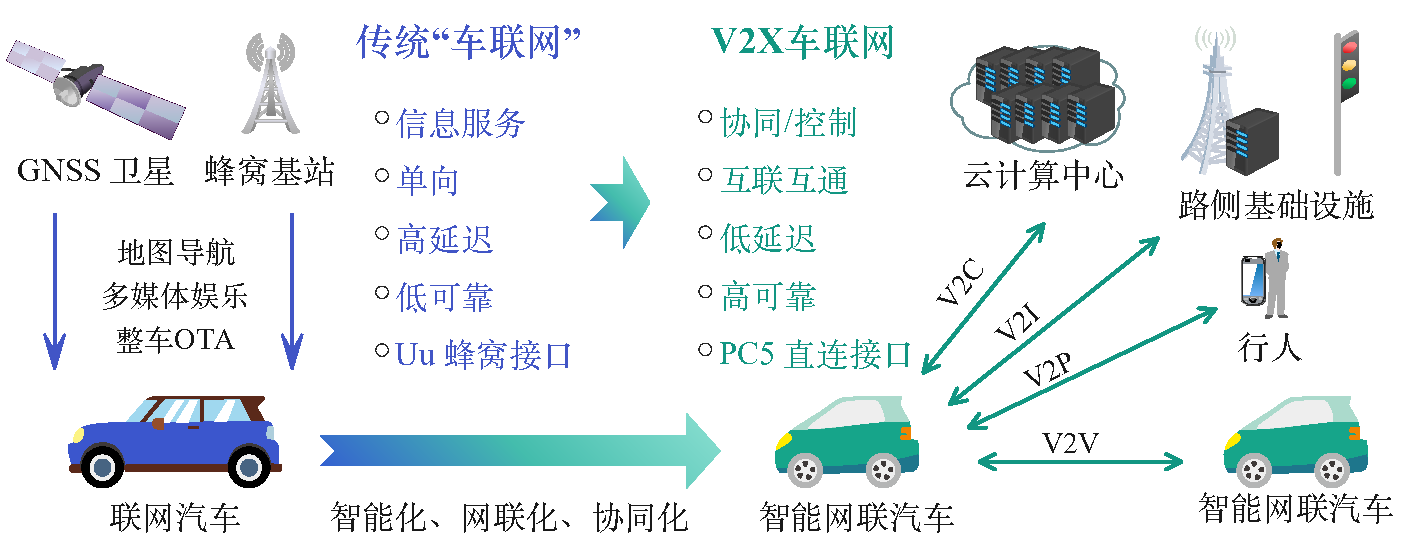
\includegraphics[width=1\columnwidth]{Fig1-1-V2X.pdf}
	\bicaption{从传统“车联网”到V2X车联网}{From traditional `connected cars' to V2X communications}
	\label{fig 1-1}
\end{figure}

车联网是物联网(Internet of Things, IoT)技术在汽车领域的应用形式。早在2G/3G移动网络时代,车联网已应用于利用全球导航卫星系统(Global Navigation Satellite System, GNSS)的定位信息为车辆提供防盗和救援服务。如今,智能网联汽车(如宝马、比亚迪、福特、通用、蔚来以及特斯拉等)都支持空中下载(Over-the-Air, OTA)技术对车机系统进行在线更新。如图 \ref{fig 1-1} 所示,随着汽车朝着智能化、网联化、协同化方向发展,传统的面向信息服务的“车联网”已经转变为与万物互联互通的V2X车联网。具体而言,V2X车联网是指多种通讯方式的融合,包括车辆间通讯(Vehicle-to-Vehicle, V2V)、车辆与行人通讯(Vehicle-to-Pedestrian, V2P)、车辆与基础设施通讯(Vehicle-to-Infrastructure, V2I)以及车辆与云端通讯(Vehicle-to-Cloud, V2C)。车联网利用实时数据分发,实现人、车、路等交通要素的协同配合,最终实现“聪明的车、智慧的路、协同的云”。此外,车联网还能促进基于单车智能的自动驾驶技术发展,通过车联网通信协助自动驾驶发现潜在危险,提升道路安全。随着我国车联网产业在政策规划、标准体系建设、关键技术研发、应用示范和基础设施建设等多方面的稳步发展,车联网的内涵和外延也在不断发展演进。依托快速落地的新型基础设施建设,车联网不仅广泛服务于智能网联汽车的辅助驾驶、自动驾驶等不同应用,还拓展服务于智慧矿山、智慧港口等企业生产环节以及智慧交通、智慧城市等社会治理领域\cite{zhong2021che}。

\begin{figure}[h]
	\centering
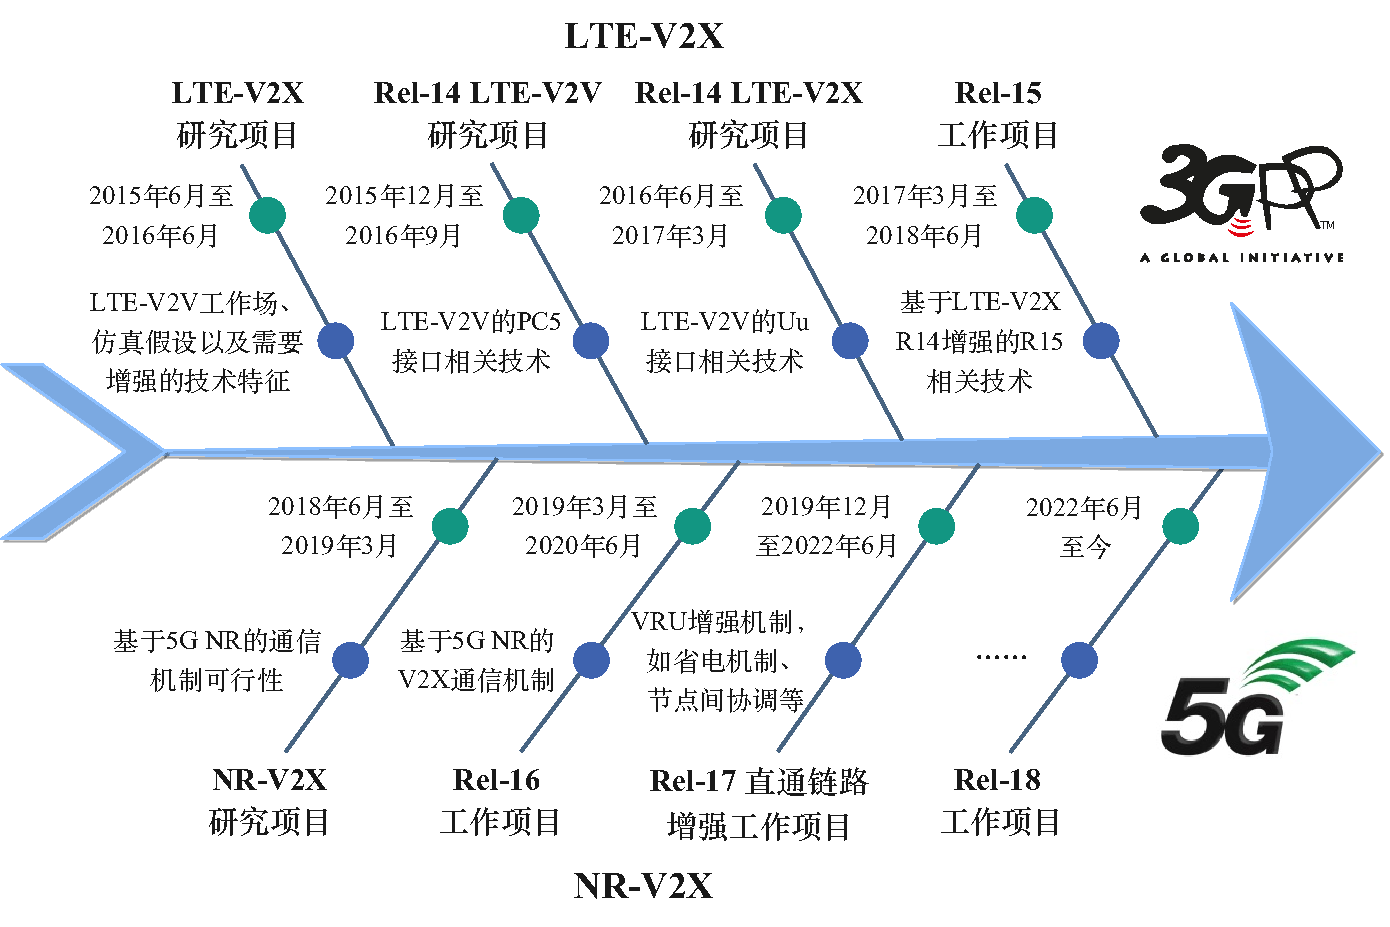
\includegraphics[width=1\columnwidth]{Fig1-2-V2X-evolution.pdf}
	\bicaption{3GPP C-V2X 标准演进}{3GPP C-V2X standard evolution}
	\label{fig 1-2}
\end{figure}

在车联网通信标准方面,电气和电子工程师协会(Institute of Electrical and Electronics Engineers, IEEE)在2003年提出了专用短距通信技术(Dedicated Short-Range Communication, DSRC)。2010年,IEEE发布了名为无线接入车载环境(Wireless Access in Vehicular Environments, WAVE)的协议栈,其中包括IEEE 802.11p、IEEE 1609.1/.2/.3/.4协议族和SAE J2735消息集字典 \cite{wu2013vehicular}。同时,基于长期演进(Long-Term Evolution, LTE)的V2X通信已形成一个完善的技术标准体系和产业链\cite{chen2016lte}。此外,IMT-2020(5G)推进组成立了C-V2X工作组,加速基于5G的V2X通信的演进。如图 \ref{fig 1-2} 所示,国际标准组织第三代合作伙伴计划(The 3rd Generation Partnership Project, 3GPP)在2018年启动基于5G新空口(New Radio, NR)的V2X标准研究,并在2020年完成了Rel-16版本的5G NR-V2X标准\cite{saad2021advancements},Rel-17版本进一步优化了功率控制、资源调度等相关技术。5G 汽车协会(5G Automotive Association, 5GAA)、下一代移动通信网络(Next Generation Mobile Network, NGMN)联盟以及5G Americas对IEEE 802.11p和C-V2X进行了技术对比,表\ref{table 1_1}显示C-V2X在传输时延、范围、速率以及可靠性等方面具有显著优势。目前,我国LTE-V2X产业蓬勃发展,与DSRC技术路线之争取得了重大进展。我国已建成基于LTE-V2X技术的完备产业链,芯片、模组、车载终端(Onboard Unit, OBU)、路侧设备(Roadside Unit, RSU)等均已成熟且经过了“三跨”“四跨”“新四跨”以及大规模测试,满足了商用部署条件。

\begin{table}[h]\small
\centering
\bicaption[C-V2X和IEEE 802.11p技术对比]{C-V2X和IEEE 802.11p技术对比\cite{cheng2021feng}}[Technical comparisons of C-V2X and IEEE 802.11p]{Technical comparisons of C-V2X and IEEE 802.11p \cite{cheng2021feng}}
\label{table 1_1}
\resizebox{\columnwidth}{!}{%
\begin{tabular}{@{}ccccc@{}}
\toprule
\begin{tabular}[c]{@{}c@{}}C-V2X\\ 技术优势\end{tabular} &
 \begin{tabular}[c]{@{}c@{}}具体技术\\ 或性能\end{tabular} &
IEEE 802.11p &
\begin{tabular}[c]{@{}c@{}}LTE-V2X\\ (3GPP R14/R15)\end{tabular} &
\begin{tabular}[c]{@{}c@{}}NR-V2X\\ (3GPP R16)\end{tabular} \\ \midrule
低时延 &
  时延 &
  不确定时延 &
  \begin{tabular}[c]{@{}c@{}}R14: 20ms\\ R15: 10ms\end{tabular} &
  3ms \\ 
\begin{tabular}[c]{@{}c@{}}低时延/\\ 高可靠\end{tabular} &
  \begin{tabular}[c]{@{}c@{}}资源分配\\ 机制\end{tabular} &
  CSMA/CA &
  \begin{tabular}[c]{@{}c@{}}支持感知+半持续\\ 调度和动态调度\end{tabular} &
  \begin{tabular}[c]{@{}c@{}}支持感知+半持续\\ 调度和动态调度\end{tabular} \\ 
\multirow{3}{*}[3.4ex]{高可靠} &
  可靠性 &
  不保证可靠性 &
  \begin{tabular}[c]{@{}c@{}}R14: \textgreater{}90\%\\ R15: \textgreater{}95\%\end{tabular} &
  支持99.999\% \\  
 &
  信道编码 &
  卷积码 &
  Turbo &
  LDPC \\ 
 &
  重传机制 &
  不支持 &
  \begin{tabular}[c]{@{}c@{}}支持HARQ,\\ 固定2次传输\end{tabular} &
  \begin{tabular}[c]{@{}c@{}}支持HARQ,\\ 传输次数灵活,\\ 最大支持32次传输\end{tabular} \\ 
\multirow{2}{*}[0ex]{\begin{tabular}[c]{@{}c@{}}更远传输\\ 范围\end{tabular}} &
  通信范围 &
  100m &
  \begin{tabular}[c]{@{}c@{}}R14: 320m\\ R15: 500m\end{tabular} &
  1000m \\  
 &
  波形 &
  OFDM &
  \begin{tabular}[c]{@{}c@{}}单载波频分复用\\ (SC-FDM)\end{tabular} &
  循环前缀(CP)-OFDM \\ 
\multirow{2}{*}[1.5ex]{\begin{tabular}[c]{@{}c@{}}更高传输\\ 速率\end{tabular}} &
  \begin{tabular}[c]{@{}c@{}}数据传输\\ 速率\end{tabular} &
  典型6Mbit/s &
  \begin{tabular}[c]{@{}c@{}}R14: 约30Mbit/s\\ R15: 约300Mbit/s\end{tabular} &
  \begin{tabular}[c]{@{}c@{}}与带宽有关,40MHz\\ 时R16单载波2层数据\\ 传输支持约400Mbit/s,\\ 多载波情况下更高\end{tabular} \\ 
 &
  调制方式 &
  64QAM &
  64QAM &
  256QAM \\ \bottomrule
\end{tabular}%
}
\end{table}

\begin{figure}[h] 
	\centering
	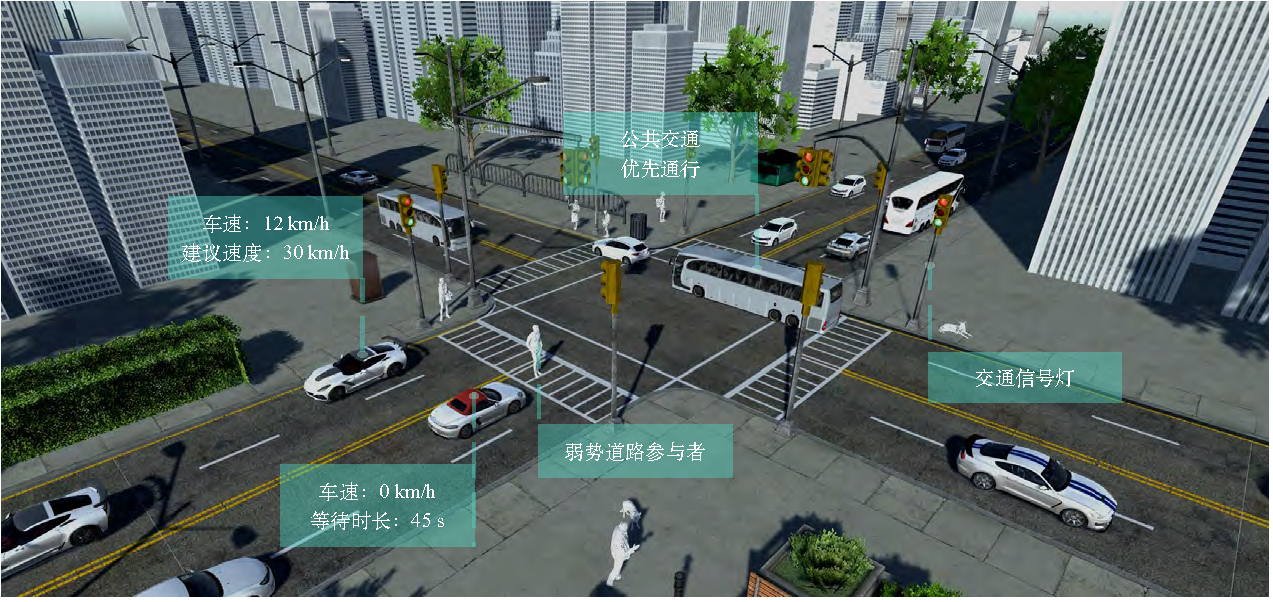
\includegraphics[width=1\columnwidth]{Fig1-3-intersection.pdf}
	\bicaption{基于车载信息物理融合的智慧全息路口}{Intelligent holographic intersection based vehicular cyber-physical fusion}
	\label{fig 1-3}
\end{figure}

如图 \ref{fig 1-3} 所示,智慧全息路口是一种基于车载信息物理融合技术的智慧交通管理系统。它通过将城市道路上的全要素进行数字化还原,为各类智能交通系统应用提供数据支撑。智慧全息路口利用道路基础设施和智能网联汽车上搭载的激光雷达、毫米波雷达、摄像头等多源传感设备,对路口进行全方位感知和全要素采集。通过传感设备实时感知交通流量、车速、车道变化等数据,并结合高精度地图呈现路口数字化上帝视角,精准刻画路口上的每一条车道、每一个交通信息灯的状态,以及每一辆车的行为轨迹。在实现路口全要素数字化还原的过程中,采用车载边缘计算技术将异构感知数据在边缘节点进行融合处理,从而提高数据处理速度,降低数据传输成本。同时,利用目标检测、目标跟踪、行为分析等算法对感知数据进行预处理,进一步提高数据准确性和精度,为后续的交通管理、交通安全和交通规划等应用提供更可靠的数据基础。

智慧全息路口不仅可以实现路口全要素数字化还原,而且可以进一步作为车载信息物理融合系统的外在展示和数据内核,支撑各种智能交通系统的应用。例如,全息路口可以为公交优先通行、绿波通行、弱势道路参与者(Vulnerable Road User, VRU)感知等 ITS 应用提供强有力的支持。在公交优先通行方面,全息路口可以根据公交车的实时位置和行驶速度,并结合路口的交通状况,提前调整信号控制策略,使公交车获得更好的通行效率和服务。在绿波通行方面,全息路口可以通过感知路口的交通流量和车速等信息,实现路口绿灯时长的自适应调整,从而实现车辆在绿波通信路段上的高效通行。在 VRU 感知方面,全息路口可以利用摄像头等传感设备或V2P通信感知VRU(如行人、自行车、残疾人等)的存在和行动轨迹,提供实时的路口状态信息和预警信息,保障弱势道路参与者的通行便利和交通安全。

通过以上讨论可知,车载信息物理融合系统是实现各类ITS应用的基础。然而,在高异构、高动态、分布式的车联网中,实现车载信息物理融合系统以满足多元ITS应用需求仍然面临着诸多问题和挑战。因此,针对以上问题和挑战,需要进一步展开全面深入的研究。具体地,首先,异构车联网亟需服务架构融合创新,并设计车载信息物理融合质量指标。未来车联网是一个多服务范式并存的高异构移动网络,因此需要研究异构车联网融合服务架构,以最大化不同服务范式的协同效应,并支持VCPS的部署实现。同时,现有研究都缺乏针对基于多源异质感知信息融合的VCPS进行整体深入的评估。因此,需要设计VCPS质量指标,并通过控制车辆感知行为与资源分配提升VCPS系统质量。其次,异构资源亟需协同优化。车联网中的通信和计算资源分布在不同的车辆和基础设施中,因此需要针对异构资源进行协同优化,支持VCPS中计算任务分布式处理,以进一步提升系统服务质量。再次,车载信息物理融合系统亟需质量-开销均衡优化。车载信息物理融合系统需要保证实时性和准确性的同时,考虑资源开销和能耗问题。因此,需要研究质量-开销均衡的优化策略,以提高系统的资源利用率的同时降低能耗。最后,亟需实现原型系统以验证VCPS性能。通过在真实车联网环境中搭建原型系统,可以进一步验证车载信息物理融合系统的可行性和有效性,为其在实际应用中提供更可靠的支持和保障。

\section{国内外研究现状}\label{section 1-3}

车载信息物理融合系统是实现各类智能交通系统应用的基础,其已成为国内外学术界研究的热点之一。本章节将对国内外相关研究工作进行梳理和总结,并从以下几个方面进行详细阐述:

\subsection{车联网服务架构研究与现状}

随着智能交通系统应用的不断涌现,传统车联网架构已无法满足大规模、高可靠、低时延的需求,因此研究人员正致力于将软件定义网络(Software Defined Network, SDN)新范式应用于车联网中。SDN通过分离数据平面和控制平面,实现了高度灵活的数据调度策略和网络功能虚拟化(Network Functions Virtualization, NFV)。Liu等人\cite{liu2016cooperative}首次将SDN概念应用于车联网中,提出了软件定义车联网(Software Defined Vehicular Network, SDVN),并在此基础上提出了基于混合V2I/V2V通信的在线协同数据调度算法,以提高数据分发的性能。Dai等人\cite{dai2018cooperative}设计了基于SDN的异构车联网中具有时间约束的时态信息服务调度方案。Luo等人\cite{luo2018sdnmac}提出了基于SDN的媒体接入(Media Access Control, MAC)协议以提高车联网的通信性能。Liu等人\cite{liu2018coding}提出了基于SDN的服务架构,并结合车辆缓存和网络编码来提高带宽利用率。Zhang等人\cite{zhang2022ac-sdvn}设计了一种解决SDVN中视频组播安全问题的安全访问控制协议,实现了多播视频请求车辆和RSU的身份认证。Zhao等人\cite{zhao2022elite}提出了一种基于智能数字孪生技术的软件定义车联网分层路由方案,克服了SDVN架构中高动态拓扑局限性。Lin等人\cite{lin2023alps}研究了一种基于SDVN的自适应链路状态感知方案,能够在信标间隔内及时获取链路状态信息,减少数据包丢失。Ahmed等人\cite{ahmed2023deep}提出了一个基于SDVN中车辆传感器负载均衡算法,并提出了一个数据包级入侵检测模型,可以跟踪并有效识别网络攻击。然而,现有大部分工作都仅是从数据分发、路由缓存、网络安全等方面展开了研究,缺乏对整体架构的深入分析。

移动边缘计算(Mobile Edge Computing, MEC)\cite{mao2017a}通过将计算、存储和网络资源靠近移动终端设备,提供更快速、更可靠的服务,同时减少网络流量消耗和服务延迟。越来越多的研究考虑将MEC范式应用在车联网环境中以提高系统实时性、可靠性和安全性。Liu等人\cite{liu2017a}首次将移动边缘计算融入车联网中,提出了车载边缘计算(Vehicular Edge Computing, VEC),并集成了不同类型的接入技术,以提供低延迟和高可靠性的通信。Lang等人\cite{lang2022cooperative}设计了一种基于区块链技术的协同计算卸载方案,以提高VEC资源的利用效率,并确保计算卸载的安全性。Liu等人\cite{liu2021fog}研究了端边云协同架构中的合作数据传播问题,并提出了一种基于Clique的算法来联合调度网络编码和数据分发。Dai等人\cite{dai2021edge}设计了一个基于自适应比特率多媒体流的VEC架构,其中边缘节点给以不同质量等级编码的文件块提供缓存和传输服务。Zhang等人\cite{zhang2022digital}提出了一种车载边缘缓存技术,动态调整边缘节点和车辆的缓存能力以提高服务的可用性。Liu等人\cite{liu2020adaptive}提出了一个两层的VEC架构,利用云、静态边缘节点和移动边缘节点来处理时延敏感性任务。Liao等人\cite{liao2021learning}研究了一种空地一体的VEC任务卸载策略,其中车辆能够学习具有多维意图的长期策略。Liu等人\cite{liu2023mobility}提出了一种利用车辆计算资源来提高VEC场景下任务执行效率的计算任务卸载方案。Liu等人\cite{liu2023asynchronous}研究了VEC中任务卸载和资源管理的联合优化问题,并采用异步深度强化学习算法来寻找最优解。然而,上述研究缺乏考虑异构车联网中不同服务架构的协同效应。

\subsection{车载信息物理融合系统质量指标研究与现状}

越来越多的研究人员聚焦于车载信息物理融合系统的预测、调度和控制技术,旨在有效提高 VCPS 系统的整体性能和可靠性。在预测技术方面,Zhang等人 \cite{zhang2021a} 提出了一种基于 VCPS 架构的车辆速度曲线预测方法,其协同 VCPS 中的不同控制单元来完成速度曲线预测。Albaba等人 \cite{albaba2021driver} 则结合深度Q网络(DQN)和层次博弈论,对高速公路驾驶场景中的驾驶员行为进行预测,其中k级推理被用来模拟驾驶员的决策过程。Zhang等人 \cite{zhang2020data} 提出了变道行为预测模型和加速预测模型。在此基础上,对车辆状态进行预测,并通过动态路由算法实现车辆之间的协同合作,以优化资源利用率和降低能源消耗。Zhou等人 \cite{zhou2021wide} 提出了一种基于宽-注意力和深度-组合模型用于交通流量预测。其中,宽-注意力模块和深度-组合模块分别用于提取全局关键特征和推广局部关键特征。在调度技术方面,Li等人 \cite{li2020cyber} 考虑了车辆移动性,并开发了一个基于物理比率-K干扰模型的广播方案,以确保通信的可靠性。Lian等人 \cite{lian2021cyber} 提出了一种基于既定地图模型路径规划的调度方法,以优化路径利用效率。在控制技术方面,Hu等人 \cite{hu2017cyber} 提出了一种燃油最优控制器,基于车队头车状态优化车辆速度和无级变速箱齿轮比。Dai等人 \cite{dai2016a} 提出了一种自主交叉路口控制机制,以确定车辆通过交叉路口的优先权。Lv等人 \cite{lv2018driving} 提出了一种自适应算法,用于三种典型驾驶方式下控制车辆加速。上述研究集中于支持 VCPS 的不同技术,如轨迹预测、路径调度和车辆控制等,虽然促进了各种 ITS 应用的实施,但是均建立在车联网中高质量物理元素建模信息可用的假设基础上,并未对车载信息物理融合质量进行定量分析。

部分研究工作侧重于利用深度强化学习(Deep Reinforcement Learning, DRL)优化 VCPS 中车辆感知和信息融合。Dong等人 \cite{dong2020spatio} 提出了一种基于 DQN 的方法,以融合在本地环境中获得的信息,从而做出可靠的车道变更决策。Zhao等人 \cite{zhao2020social} 设计了一个基于近似策略优化(Proximal Policy Optimization, PPO)的社会意识激励机制,以得出最佳的长期车辆感知策略。Mika等人 \cite{mlika2022deep} 提出了一个基于深度确定性策略梯度(Deep Deterministic Policy Gradient, DDPG)的解决方案,通过调度资源块和广播覆盖来优化信息时效性。然而,上述算法不能直接应用于 VCPS 中的协同感知和异构信息融合,并且,当考虑到多辆车场景时,上述算法并不适用。另一方面,部分研究对 VCPS 中的信息质量进行了评估。Liu等人 \cite{liu2014temporal} 提出了一种用于 VCPS 中时态数据传播的调度算法,其在实时数据传播和及时信息感知之间取得了平衡。Dai等人 \cite{dai2019temporal} 提出了一种进化多目标算法,以提高信息质量和改善数据到达率。Liu等人 \cite{liu2014scheduling} 提出了两种在线算法,通过分析传播特性来调度不同一致性要求下的时态数据传播。Rager等人 \cite{rager2017scalability} 开发了一个刻画真实网络随机性的框架,对随机数据负载进行建模以提高信息质量。Yoon等人 \cite{yoon2021performance} 提出了一个车联网中的合作感知框架,考虑到通信损耗和车辆随机运动,以获得车辆的精确运动状态。上述研究主要聚焦于 VCPS 中数据及时性、准确性或一致性方面的信息质量评估。然而,这些研究仅考虑了同质数据项层面的质量评估,没有针对车载信息物理融合进行质量评估。

\subsection{车联网资源分配与任务卸载研究与现状}

车联网中的资源分配一直是学术界的研究热点 \cite{noor-a-rahim2022a},大量研究人员针对车联网中通信资源分配进行了深入研究。He等人 \cite{he2022meta} 设计了一种动态车联网资源管理框架,其采用马尔可夫决策过程(Markov Decision Process, MDP)和分层强化学习相结合的方法,可以显著提高资源管理性能。Lu等人 \cite{lu2021user} 提出了一种基于用户行为的虚拟网络资源管理方法,以进一步优化车联网通信。Peng等人 \cite{peng2020deep} 提出了一种针对车联网的资源管理方案,通过应用 DDPG 方法解决了多维资源优化问题,实现了资源快速分配,并满足了车联网服务质量(Quality of Service, QoS)要求。Wei等人 \cite{wei2022multi} 针对车联网云计算中的资源分配问题,从提供者和用户双重视角出发,提出了一种改进的 NSGA-II 算法来实现多目标优化。Peng等人 \cite{peng2021multi} 研究了无人机辅助车联网中的多维资源管理问题,并提出了一种基于多智能体深度确定性策略梯度(Multi-Agent Deep Deterministic Policy Gradient, MADDPG)的分布式优化方法,实现了车辆资源联合分配。为了进一步提高频谱利用率和支持更多车辆接入,部分研究将非正交多址接入(Non-Orthogonal Multiple Access, NOMA)技术融入车联网中。Patel等人 \cite{patel2021performance} 评估了基于 NOMA 的车联网通信容量,其数值结果显示,NOMA 通信容量比传统的正交多址接入(Orthogonal Multiple Access,OMA)高出约20\%。Zhang等人 \cite{zhang2021centralized} 利用基于图的匹配方法和非合作博弈(Non-Cooperative Game,NCG)分布式功率控制,为NOMA车联网开发了一个集中的两阶段资源分配策略。Zhu等人 \cite{zhu2021decentralized} 提出了一种考虑随机任务到达和信道波动的最优功率分配策略,以最大化长期的功率消耗和延迟。Liu等人 \cite{liu2019energy} 在基于 NOMA 的车联网中,提出了基于交替方向乘子法(Alternating Direction Method of Multipliers,ADMM)的功率分配算法。然而,上述研究主要是基于单边缘节点的情况,无法处理不同边缘节点之间的相互干扰情况。因此,仍然需要探索更加复杂的多边缘节点环境下的资源分配策略,以提高车联网的性能和可靠性。


随着车载边缘计算的发展,大量研究专注于 VEC 中的任务卸载和资源分配。其中,Liu等人\cite{liu2021rtds}提出了一种多周期任务卸载的实时分布式方法,通过评估 VEC 中的移动性感知通信模型、资源感知计算模型和截止时间感知奖励模型。Shang等人\cite{shang2021deep}研究了节能的任务卸载,并开发了一种基于深度学习的算法来最小化能耗。为了最小化执行延迟、能源消耗和支付成本的加权和,Liu等人\cite{liu2022a}提出了一种结合 ADMM 和粒子群优化(Particle Swarm Optimization, PSO)的任务卸载算法。Chen等人\cite{chen2020robust}设计了一种带有故障恢复功能的计算卸载方法,以减少能源消耗并缩短服务时间。为了实现超高可靠低时延通信(ultra-Reliable and Low-Latency Communication, uRLLC)服务需求下最大化吞吐量,Pan等人\cite{pan2022asynchronous}提出了一种基于异步联合 DRL 的计算卸载方案。Zhu等人\cite{zhu2022a}提出了一种用于智能反射面(Intelligent Reflecting Surface, IRS) 辅助下的 VEC 的动态任务调度算法,优化有限资源分配并考虑了车辆的移动模式、传输条件和任务大小以及并发传输之间的相互干扰。此外,部分研究聚焦于采用多智能体强化学习(Multi-Agent Deep Reinforcement Learning, MADRL)算法的任务卸载和资源分配。Alam等人\cite{alam2022multi}开发了一种基于 DRL 的多智能体匈牙利算法,用于 VEC 中的动态任务卸载以满足延迟、能耗和支付费用需求。Zhang等人\cite{zhang2021adaptive}提出了一种基于 MADDPG 的边缘资源分配方法,在严格延迟约束下最小化车辆任务卸载成本。为了同时满足严格延迟要求和最小带宽消耗,He等人\cite{he2021efficient}提出了一种多智能体行动者-评论家(Multi-Agent Actor-Critic, MAAC)算法,用于车辆带宽分配。然而,以上研究工作都没有考虑实时任务卸载和通信/计算资源分配的协同优化。

部分研究专注于VEC的联合通信和计算资源分配。Cui等人\cite{cui2021reinforcement}提出了一种多目标的强化学习方法,通过协同通信和计算资源的分配来减少系统延迟。Han等人\cite{han2020reliability}设计了基于动态规划(Dynamic Programming,DP)的资源分配方法,实现了耦合车辆通信和计算资源的可靠性计算。Xu等人\cite{xu2021socially}采用契约理论为每个潜在的内容供应商和内容请求者分配通信和计算资源。少数研究者研究了联合任务卸载和资源分配。Dai等人\cite{dai2021asynchronous}提出了一个异步的DRL算法,实现了异构服务器数据驱动的任务卸载。此外,Dai等人 \cite{dai2022a}开发了一种概率计算卸载方法,根据边缘节点的计算分配概率进行计算卸载的独立调度。Nie等人\cite{nie2021semi}提出了一种MADRL算法,在无人机辅助VEC中联合优化资源分配和功率控制。然而,现有研究主要基于集中式调度,通信开销和调度复杂性较高,不适用于大规模的车联网。

\subsection{车载信息物理融合中质量/开销优化研究与现状}

近年来,许多研究人员致力于提高车载信息物理融合中的 QoS,以提升 ITS 应用的用户体验。其中,Wang等人\cite{wang2016offloading}提出了一种组合优化方法,旨在减少移动数据流量的同时满足 VCPS 中面向 QoS 的服务需求。Jindal等人\cite{jindal2018sedative}提出了一种基于 SDN 和深度学习的 VCPS 网络流量控制方案,成功解决了网络流量管理问题。Zhu等人\cite{zhu2022joint}设计了一种基于双时间尺度 DRL 的方法,以优化基于车辆编队的 VCPS 中的车辆间距和通信效率,同时满足 V2I 通信的 QoS 要求。Wang等人\cite{wang2023a}提出了一种集群式车辆通信方法,通过公交车聚类和混合数据调度实现了从公交车到普通车辆的有效数据传播并满足了严格和个性化的 QoS 需求。此外,Chen等人\cite{chen2021qos}致力于解决 IRS 辅助车联网中的频谱共享问题,通过优化车辆的发送功率、多用户检测矩阵、频谱重用以及 IRS 反射系数等参数,提高车联网通信的服务质量。Lai等人\cite{lai2017a}提出了一种基于 SDN 的流媒体传输方法,根据用户移动信息、播放缓冲区状态和当前网络信号强度向 SDN 控制器提供流媒体传输策略,以实现最小延迟和更好的 QoS。Tian等人\cite{tian2022multiagent}则设计了一种基于 MADRL 的资源分配框架,以共同优化信道分配和功率控制,满足车联网中的异构 QoS 需求。同时,Zhang等人\cite{zhang2020hierarchical}研究了 MEC 车联网中联合分配频谱、计算和存储资源问题,并利用 DDPG 解决该问题,以满足 ITS 应用的 QoS 要求。Sodhro等人\cite{sodhro2020ai}建立了可靠和延迟容忍的无线信道模型和多层边缘计算驱动的框架,有效提升了车联网服务质量。

另一方面,部分研究人员致力于降低 VCPS 中的各类开销。例如,Zhao等人\cite{zhao2021a}设计了一种基于 SDN 和无人机(Unmanned Aerial Vehicle, UAV)辅助的车辆计算卸载优化框架,其中采用了UAV辅助车辆计算成本优化算法以最小化系统成本。Zhang等人\cite{zhang2019hybrid}提出了一种基于蚁群优化和三个变异算子的算法,用于优化具有灵活时间窗口的多目标车辆路径,以最小化行驶成本和车辆固定成本。Ning等人\cite{ning2020when}则针对5G车联网中无线频谱有限的问题,构建了一个智能卸载框架,联合利用蜂窝频谱和未许可频谱来满足车辆需求,并在考虑时延限制的基础上使成本最小化。Tan等人\cite{tan2019twin}提出了一种基于人工智能(Artificial Intelligence,AI)的多时间尺度框架的联合通信、缓存和计算策略,其中考虑了车辆的移动性和硬服务截止期限约束,并实现了最大化网络成本效益。Hui等人\cite{hui2022collaboration}提出了一种协作自动驾驶方案,并通过联盟博弈机制来确定最佳车辆分簇,以最小化每个簇的计算成本和传输成本。虽然上述研究对 VCPS 系统中的开销进行了深入研究,但这些研究并未考虑车载信息物理融合系统构建的质量和开销。因此,需要进行对 VCPS 系统本身的评估与质量-开销均衡的深入研究。

\subsection{智能交通系统安全相关应用研究与现状}

随着城市化进程的加速和交通流量的不断增加,ITS 安全相关应用的部署可以大幅提高道路交通的安全性。因此,许多研究人员针对驾驶员状态监测、驾驶行为分析、交通监测等方面进行了研究。Mugabarigira等人\cite{mugabarigira2023context}提出了一种基于车辆行为追踪和驾驶风险分析的导航系统,可提高城市道路上车辆的安全性。Chang等人\cite{chang2018design}提出了一种基于可穿戴智能眼镜的疲劳驾驶检测系统,能够实时检测驾驶员的疲劳或嗜睡状态。Dutta等人\cite{dutta2022design}提出了一种基于凸优化的鲁棒分布式状态估计系统,可保护连接车辆的传感器数据免受拒绝服务(Denial-of-Service, DoS)或虚假数据注入(False Data Injection, FDI)攻击。Wang等人\cite{wang2021deep}提出了一种基于深度学习加速器嵌入式平台的鲁棒雨滴检测系统,并利用检测结果自动控制汽车雨刷。Sun等人\cite{sun2022toward}提出了一种有效的交通估计系统,可通过与过往车辆通信并记录其出现情况来实现自动交通测量,为ITS提供关键信息。

部分研究工作从车辆控制、车辆编队控制、路口交通流控制等多个层面对 ITS 安全相关应用展开了深入分析。Zhang等人\cite{zhang2021data}提出了一种分布式安全巡航控制系统,利用历史数据建立了车辆行为预测模型和动态驾驶系统模型,并设计了考虑合并行为概率的安全跟驰控制策略。Zhao等人\cite{zhao2022resilient}提出了一个具有鲁棒性的车辆编队控制系统,并设计了一种在多重干扰和 DoS 攻击下恢复机制,降低 DoS 攻击对 VCPS 的不利影响。Pan等人\cite{pan2023privacy}设计了一种面向车联网的车队隐私保护集结控制系统,通过采样数据的动态加密和解密方案,使得车队之间的通信数据得以保密。Li等人\cite{li2021confidenitality}介绍了一种低延迟协作安全车辆编队数据传输系统,采用无线电信道相关性的协作密钥协商协议以保证数据传输的安全。Kamal等人\cite{kamal2021control}提出了一种多智能体路口交通流控制系统,利用随机梯度方法计算交通信号灯持续时间。Lian等人\cite{lian2021cyber}提出了基于交通控制的智能物流系统,并设计了改进的A*路径规划算法以实现主动调度和碰撞避免。

作为典型 ITS 安全相关应用,车辆碰撞预警已引起广泛研究人员的关注。目前,大多数车辆碰撞预警系统都是基于超声波雷达或激光雷达等测距传感器的。Song等人\cite{song2018real}提出了一种实时障碍物检测和状态分类方法,该方法融合了立体摄像头和毫米波雷达,并结合车辆运动模型,通过多个模块感知环境,能够准确快速地判断出“潜在危险”物体。Wu等人\cite{wu2019series}提出了一种77GHz车辆碰撞预警雷达系统短程天线,该系统采用补丁阵列天线作为基本结构,并采用多层板设计技术使其尺寸更小。然而,这些方案都存在非视距(Non-Line-Of-Sight, NLOS)的问题,即在障碍物遮挡情况下基于视距(Line-Of-Sight, LOS)的方法不再适用。近年来,随着计算机视觉的发展,一些研究集中在基于摄像头实时视频流的碰撞检测上。Wang等人\cite{wang2016vision}提出了一种新颖的车辆制动行为检测方法,利用安装在挡风玻璃上的摄像头来捕获前车信息,以避免与前方车辆相撞。Song等人\cite{song2018lane}提出了一种轻量级的基于立体视觉的车道检测和分类系统,以实现车辆的横向定位和前向碰撞预警。然而,基于计算机视觉的方法需要大量数据传输和密集计算,这使得系统的性能无法得到实时响应。另一方面,部分研究考虑了通过 V2X 通信实现碰撞预警。Hafner等人\cite{hafner2013cooperative}基于 V2V 通信技术实现了一种分布式算法,用于交叉路口的车辆协同防撞。Gelbar等人\cite{gelbal2017elastic}提出了一个基于 V2X 通信的车辆碰撞预警和避免系统。然而,无线通信中的传输时延和数据包丢失等内在特征是不可避免的,对于车辆碰撞预警系统也是不可忽视的。这使得在真实复杂车联网环境中实现实时和可靠的安全关键型服务变得更加困难。

\section{研究目标与研究内容}\label{section 1-4}

\subsection{研究目标}

本文针对异构车联网高动态物理环境、动态分布式车联网节点资源、智能交通系统多元应用需求,以及真实复杂性车联网通信环境所带来的挑战,从架构融合与指标设计、协同资源优化、质量-开销均衡,以及原型系统实现四个方面对车载信息物理融合系统展开研究。本文的研究目标如下:

\circled{1} 针对车联网高异构、高动态、高分布式等特征,提出融合软件定义网络和移动边缘计算的车联网分层服务架构,并实现视图质量的量化评估,是车载信息物理融合系统的架构基础与驱动核心。首先,结合软件定义网络、网络功能虚拟化和网络切片等关键思想,提出车联网分层服务架构,以支持 VCPS 的部署与实现。其次,提出基于多类 M/G/1 优先队列的感知信息排队模型。进一步,针对边缘视图对于感知信息的时效性、完整性以及一致性需求,设计 VCPS 质量指标,并形式化定义视图质量优化问题。最后,提出基于差分奖励的多智能体强化学习视图质量优化策略,实现高效实时的边缘视图构建。

\circled{2} 针对车联网中异构节点资源、动态拓扑结构与无线通信干扰等特征,实现基于边缘协同的异构资源优化,是进一步优化 VCPS 服务质量的技术支撑。首先,面向 NOMA 车联网的车载边缘计算环境,考虑 V2I 通信中边缘内与边缘间干扰,提出 V2I 传输模型,并考虑边缘协作提出任务卸载模型。其次,形式化定义协同资源优化问题,并将其分解为任务卸载与资源分配两个子问题。最后,提出基于博弈理论的多智能体强化学习算法的资源优化策略,具体地,基于多智能体强化学习实现任务卸载博弈的纳什均衡,并基于凸优化理论提出最优资源分配方案,实现最大化资源利用效率。

\circled{3} 针对多元智能交通系统应用对于视图质量/开销的差异性需求,实现车载信息物理融合质量-开销均衡,是实现高质量低成本车载信息物理融合的理论保障。首先,考虑视图中信息的及时性与一致性需求,建立车载信息物理融合质量模型。其次,考虑视图构建中感知信息的冗余度、感知开销与传输开销,建立车载信息物理融合开销模型。最后,提出基于多目标多智能体强化学习的质量与开销均衡策略,实现高质量低成本可扩展车载信息物理融合。

\circled{4} 针对真实复杂性车联网通信环境中验证车载信息物理融合的需求,设计并实现基于车载信息物理融合的原型系统,是验证车载信息物理融合的必要手段。首先,提出基于视图修正的碰撞预警算法。其次,搭建基于 C-V2X 设备的硬件在环测试平台,实现硬件在环性能验证。最后,在真实车联网环境中,实现基于车载信息物理融合的超视距碰撞预警原型系统,进一步验证所提算法和系统模型的可行性和有效性。

\subsection{研究内容}

本文致力于研究车载信息物理融合系统,主要研究内容及关系如图 \ref{fig 1-4} 所示。
首先,面向异构车联网高动态物理环境,融合不同的计算范式与服务架构,并实现有效的数据获取与建模评估是车载信息物理融合的架构基础与驱动核心。
因此,本文将首先研究如何设计融合软件定义网络和移动边缘计算的车联网分层服务架构,在此基础上,研究如何评估并提高车载边缘侧所构建的逻辑视图质量。
其次,面向动态分布式车联网节点资源,高效的任务调度与资源分配是车载信息物理融合的技术支撑。
因此,本文将研究如何实现异构资源协同优化,提高资源利用效率。
面向多元智能交通系统应用需求,实现车载信息物理融合质量-开销均衡是车载信息物理融合的理论保障。
因此,本文将进一步研究车载信息物理融合质量/开销模型及其均衡优化策略。
最后,面向真实复杂性车联网通信环境,基于车载信息物理融合设计并实现具体系统原型是车载信息物理融合的验证手段。
因此,本文将更进一步设计及实现基于车载信息物理融合的超视距碰撞预警原型系统,实现理论与系统的相互促进。
本文具体研究内容如下:

\begin{figure}[h] 
	\centering
	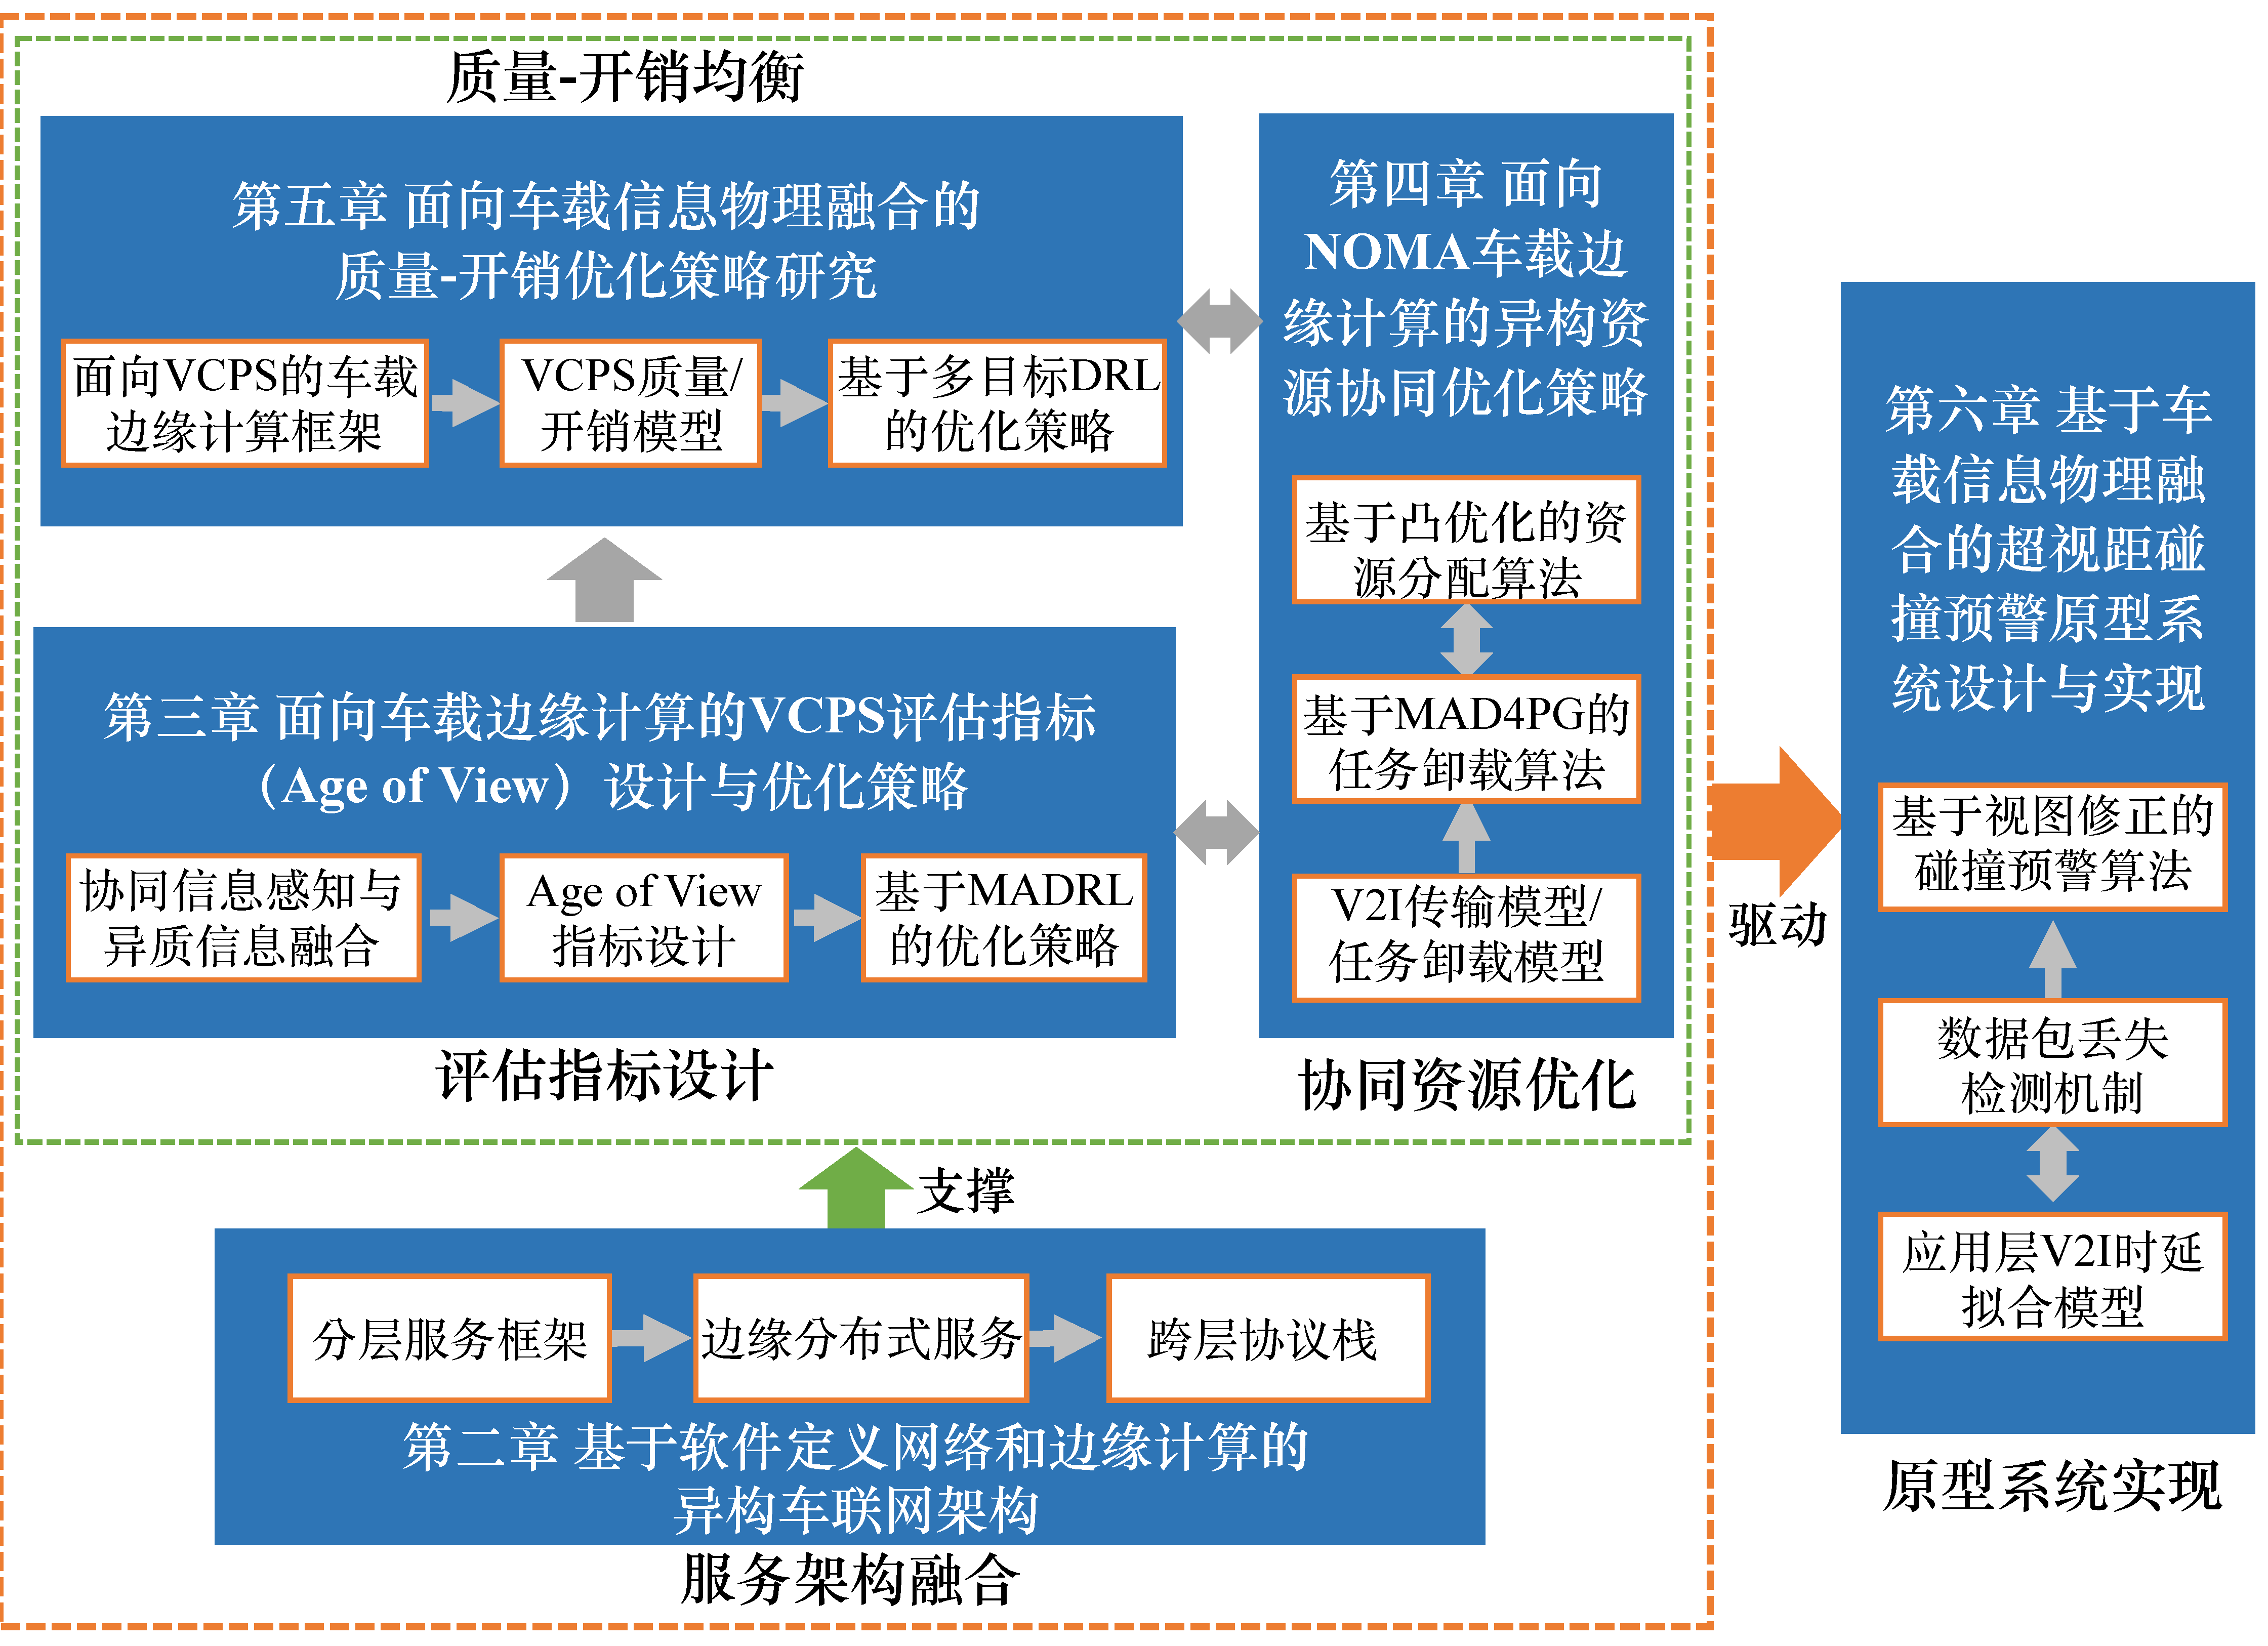
\includegraphics[width=1\columnwidth]{Fig1-4-content.pdf}
	\bicaption{主要研究内容}{Main research content}
	\label{fig 1-4}
\end{figure}

\circled{1} 基于分层车联网架构的车载信息物理融合质量指标设计与优化。
考虑车联网环境中的网络资源的高异构性、车联网物理环境分布式时变性、拓扑结构的高动态性,以及车辆节点感知能力差异性等关键特征,本文将研究融合软件定义网络和移动边缘计算的分层车联网服务架构。进一步,本文将重点研究基于分层服务架构的分布式感知与异质信息融合模型,考虑信息的多维需求,研究车载信息物理融合质量指标设计。在此基础上,研究基于差分奖励多智能体强化学习的边缘视图优化策略。

\circled{2} 面向车载信息物理融合的通信与计算资源协同优化关键技术。
考虑车联网高动态环境与高异构分布式资源,本文将引入NOMA技术提升车联网频谱资源利用效率,并提出基于边缘协同的异构资源优化策略。本文将重点研究 V2I 传输与任务卸载模型,并在此基础上,研究基于博弈理论多智能体深度强化学习的异构资源协同优化策略,具体地,基于凸优化理论,研究通信资源最优分配策略,并基于任务卸载势博弈模型,研究基于多智能体深度强化学习的任务卸载算法。

\circled{3} 面向车载信息物理融合的质量-开销均衡优化关键技术。
考虑智能交通系统中多元应用需求,本文将研究车联网中不同交通要素的视图质量与开销模型,并提出车载信息物理融合质量-开销均衡优化策略。本文将综合考虑视图的建模质量,包括信息的及时性与一致性,研究车载信息物理融合质量模型,并考虑视图的构建开销,包括信息冗余度、感知开销与传输开销,研究车载信息物理融合开销模型。在此基础上,研究基于多目标多智能体深度强化学习的车载信息物理融合质量-开销均衡优化策略。

\circled{4} 面向车载信息物理融合系统的超视距碰撞预警原型系统设计与实现。
考虑真实复杂性车联网通信环境,本文将研究基于车载信息物理融合系统的超视距碰撞预警原型系统设计与实现。具体地,本文将研究C-V2X应用层时延拟合模型和数据丢包检测机制,并研究基于视图修正的碰撞预警算法。在此基础上,研究基于 C-V2X 通信设备的硬件在环试验平台搭建方案,并研究在真实车联网环境中基于车载信息物理融合的超视距碰撞预警原型系统实现方案。

\section{论文的特色与创新之处}\label{section 1-6}

区别于目前仅专注于车联网通信协议、服务架构、资源分配和智能应用等方面的研究,本文旨在从实际需求出发,分析当前面临的挑战,并在车载信息物理融合系统的四个方面进行深入研究:架构基础与驱动核心、技术支撑、理论保障与验证手段。本文的具体特色在于:
a) 针对异构车联网高动态物理环境和信息感知的时效性与准确性需求,考虑到感知信息时变性、车辆节点移动性和感知能力差异性所带来的挑战,研究如何将基于SDN的集中控制和基于移动边缘计算的分布式调度有机结合,并在边缘侧建立有效的逻辑视图,为车载信息物理融合系统提供架构基础和驱动核心。
b) 针对动态分布式车联网节点资源,考虑节点异构资源的动态性、分布性和无线通信中边缘内和边缘间干扰所带来的挑战,研究如何实现边缘协同,最大化异构资源利用效率,为车载信息物理融合系统提供技术支撑。
c) 针对多元智能交通系统的应用需求,考虑到车联网中不同交通要素视图质量和开销需求差异所带来的挑战,研究如何实现车载信息物理融合系统的质量-开销均衡,为车载信息物理融合系统提供理论保障。
d) 针对真实复杂的车联网通信环境,考虑基于真实C-V2X通信设备部署和实现原型系统所带来的挑战,研究基于车载信息物理融合的超视距碰撞预警系统的原型设计和实现,为车载信息物理融合系统提供系统验证。
本文的主要创新点概括如下:

\circled{1} 提出融合软件定义网络与移动边缘计算的车联网分层服务架构,并定义边缘视图概念,率先设计视图评估指标并建立视图质量评估模型,提出分布式信息感知与异质信息融合的边缘视图构建机制:现有车联网服务架构相关研究主要关注于单一范式的实践应用,难以适用于具有大规模数据服务需求的下一代车联网场景与支撑车载信息物理融合系统。同时,现有研究重点关注于针对单一类型的时态数据建模与调度,难以面向车载信息物理融合系统形成有效的数据支撑。因此,本文首先综合考虑高移动数据节点、高动态网络拓扑、高异构通信资源、高分布式系统环境等车联网特征,设计基于 SDN 集中控制与基于 MEC 分布式服务有机结合的异构车联网架构。在此基础上,综合考虑感知信息的时效性、完整性与一致性,定义车联网边缘视图概念,建立针对视图质量的量化评估模型,并提出基于差分奖励的多智能体强化学习的边缘视图优化策略,实现车载边缘计算环境下的有效信息物理融合。

\circled{2} 提出基于边缘协同的异构资源协同优化策略,打破传统的单一资源优化模式:现有面向车联网资源优化策略的研究主要集中于单一资源(如通信、计算)的优化,难以满足车联网节点在不同任务中对异构资源的需求。因此,本文首先针对协同资源优化问题进行分解为任务卸载与通信资源分配两个子问题。进一步,提出基于博弈理论的多智能体深度强化学习的协同资源优化策略。具体地,将任务卸载子问题建模为势博弈模型,并证明其具有纳什均衡存在性与收敛性。最后,针对任务卸载博弈,提出基于多智能体深度强化学习的任务卸载策略。对于通信资源分配,提出基于凸优化的通信资源分配策略,实现最大化异构资源利用效率。

\circled{3} 定义车载信息物理融合系统质量与开销模型,提出基于多目标强化学习的优化策略,该策略注重实现 VCPS 质量最大化的同时同时满足 VCPS 开销最小化的要求:现有研究主要关注于基于车载信息物理融合系统的应用,而忽略了车载信息物理融合的质量与开销。因此,本文首先面向多元智能交通系统应用的差异性需求,针对车联网中不同要素建立视图模型。进一步,提出面向车联网中不同实体要素视图的质量/开销模型。最后,提出基于多目标多智能体深度强化学习的车载信息物理融合系统质量-开销均衡优化策略,以实现高质量、低成本和可扩展的车载信息物理融合。

\circled{4} 设计并实现面向车载信息物理融合的超视距碰撞预警原型系统,并在真实车联网环境下验证所提算法与系统模型:现有研究主要关注于基于仿真平台的实验验证,难以满足基于车载信息物理融合的实际 ITS 应用在真实车联网环境下的验证需求。因此,本文首先建立基于C-V2X的无线传输时延拟合模型。进一步,提出数据包丢失检测机制,并设计基于视图修正的碰撞预警算法。最后,搭建基于C-V2X设备的硬件在环试验平台,并在真实车联网环境中实现超视距碰撞预警系统原型,验证车载信息物理融合的可行性和有效性。

\section{论文的组织结构}\label{section 1-7}
本文围绕车载信息物理融合系统相关问题展开了研究。
具体地,本文将结合车联网高异构、高动态、分布式特征与智能交通系统多元需求,从车联网的架构融合与指标设计、资源协同优化、质量-开销均衡,以及原型系统实现方面进行理论研究与技术创新。
本文共分为六个章节,详细内容安排如下:

第一章,绪论。首先,介绍了车载信息物理融合系统的研究背景和国内外相关研究现状。其次,阐述了本文的研究目标与详细内容。最后,总结了本文的组织结构。

第二章,基于分层车联网架构的车载信息物理融合质量指标设计与优化。首先,设计了融合软件定义网络和移动边缘计算的分层服务架构,并提出了分布式感知与异质信息融合场景。在此基础上,设计了 Age of View 指标, 并形式化定义了车载信息物理融合质量最大化问题。其次,提出了基于差分奖励的多智能体深度强化学习的视图质量优化策略。最后,构建了实验仿真模型并验证了所提指标与算法的优越性。

第三章,面向车载信息物理融合的通信与计算资源协同优化关键技术。首先,提出了协同通信与计算卸载场景。其次,建立了V2I传输模型和任务卸载模型,在此基础上,形式化定义了协同资源优化问题。再次,提出了基于博弈理论的多智能体强化学习的资源优化策略。最后,建立了实验仿真模型并验证了所提算法的优越性。

第四章,面向车载信息物理融合的质量-开销均衡优化关键技术。首先,提出了协同感知与V2I上传场景。其次,建立了了VCPS系统质量和系统开销模型,在此基础上,形式化定义了最大化系统质量与最小化系统开销的双目标优化问题。再次,提出了基于多目标的多智能体深度强化学习的质量-开销均衡策略。最后,构建了实验仿真模型并验证了所提算法的优越性。

第五章,面向车载信息物理融合的超视距碰撞预警原型系统设计及实现。首先,提出了超视距碰撞预警场景。其次,设计了基于视图修正的车辆碰撞预警算法。再次,搭建了基于 C-V2X 设备的硬件在环试验平台。最后,在真实车联网环境中,实现了基于车载信息物理融合的超视距碰撞预警系统原型,验证了车载信息物理融合的可行性与有效性。

第六章,总结与展望。总结了全文研究内容,并讨论了后续研究计划。







\chapter[基于分层车联网架构的车载信息物理融合质量指标设计与优化]{基于分层车联网架构的车载信息物理融合质量指标\\设计与优化}
本章将研究基于分层车联网架构的车载信息物理融合系统质量指标设计与优化。
本章内容安排如下:
\ref{section 2-1} 节是本章的引言,介绍了车联网服务架构与车载信息物理融合系统质量指标的研究现状、目前研究的不足,以及本章的主要贡献。
\ref{section 2-2} 节阐述了分层车联网架构设计。
\ref{section 2-3} 节介绍了分布式感知与异质信息融合场景。
\ref{section 2-4} 节设计了车载信息物理融合质量指标并形式化定义VCPS质量优化问题。
\ref{section 2-5} 节提出了基于差分奖励的多智能体强化学习算法用以优化VCPS质量。
\ref{section 2-6} 节搭建了仿真实验模型并进行了性能验证。
\ref{section 2-7} 节总结了本章的研究工作。

\section{引言}\label{section 2-1}

随着无线通信技术的蓬勃发展,车联网正逐步成为支持下一代智能交通系统的关键技术。随着 C-V2X 通信、大数据和人工智能的发展,汽车行业的下一场革命即将到来。回顾过去十余年手机的发展历程,可以看到手机已经从传统的通话和信息传递工具转变为具有社交、导航、多媒体娱乐等诸多功能的智能设备。类似于手机的发展,汽车不再仅是单纯的运输工具,而且将朝着智能化、网联化、协同化方向演进,成为支撑各种智能交通系统应用的关键。软件定义网络\cite{li2021zhi}和移动边缘计算\cite{liu2022fedcpf}新兴范式的涌现,为车联网提供了支持高密度车辆通信、海量数据传输、自适应计算卸载,以及逻辑集中控制等功能的解决方案。传感技术和车联网的最新进展也推动了车载信息物理融合系统的发展,并进一步推动下一代智能交通系统的实现。在VCPS中,交通灯信号、车辆位置、点云数据和监控视频等异质信息可以被车辆分布式感知并上传至边缘节点。边缘节点基于车辆感知信息进行融合,构建反映车联网中各元素的物理状态的逻辑映射,其被称为逻辑视图。因此,本章致力于提出一种新颖的分层车联网服务架构,以最大化软件定义网络和移动边缘计算范式的协同效应,并支撑实时、可靠的车载信息物理融合系统。在此基础上,考虑了车载分布式感知与异质信息融合场景,设计了车载信息物理融合质量指标与相应的调度算法,以最大化车载信息物理融合质量。

研究人员对车联网服务架构进行了深入研究。自2016年Liu等人\cite{liu2016cooperative}首次将SDN应用于车联网以来,大量研究人员围绕软件定义车联网进行了研究\cite{dai2018cooperative, luo2018sdnmac, liu2018coding, zhang2022ac-sdvn, zhao2022elite, lin2023alps, ahmed2023deep}。然而,现有的大部分工作仅仅是在软件定义车联网架构的基础上,从数据分发、路由缓存、数据安全等方面展开了研究,并没有对整体架构进行深入分析。另一方面,越来越多的研究在车联网环境中考虑将移动边缘计算范式应用于系统,以提高实时性、可靠性和安全性\cite{liu2017a, lang2022cooperative, liu2021fog, dai2021edge, zhang2022digital, liu2020adaptive, liao2021learning, liu2023mobility, liu2023asynchronous}。然而,上述研究并没有考虑在异构车联网中最大化不同服务架构的协同效应。研究人员围绕车联网中的数据传播 \cite{liu2021fog, singh2020intent}、信息缓存 \cite{zhang2022digital, dai2020deep, su2018an} 和任务卸载 \cite{shang2021deep, liao2021learning} 方面展开了深入研究。然而,现有研究工作都没有考虑分布式感知和异质信息融合的协同效应。部分研究人员对VCPS中的预测 \cite{zhang2019a, zhang2020data}、调度 \cite{li2020cyber, lian2021cyber} 和控制 \cite{dai2016a, hu2017cyber, lv2018driving}技术进行了大量的研究,并促进了各种ITS应用的实现。然而,上述研究都是基于边缘/云节点能够收集足够且可靠信息的基础上。部分研究聚焦于VCPS中的信息质量评估\cite{liu2014temporal, dai2019temporal, liu2014scheduling, rager2017scalability, yoon2021performance}。然而,大部分研究工作只评估了数据项层面的质量,而忽略了对异质信息融合的质量评估。部分研究专注于车联网中使用深度强化学习的车辆传感和信息融合\cite{dong2020spatio, zhao2020social, mlika2022deep},但并不适用于多车场景。少数研究将多智能体DRL应用于车联网中\cite{kumar2022multi, he2021efficient}。然而,这些解决方案都不能直接应用于车载信息物理融合系统中的分布式感知和异质信息融合。

基于以上分析,本章针对分层架构和质量指标进行了协同研究,在分层车联网架构基础上实现分布式感知和异质信息融合,并提高车载信息物理融合质量。本章的主要贡献如下:第一,提出了融合软件定义网络和移动边缘计算范式的车联网分层服务架构。该架构包含应用层、控制层、虚拟层和数据层,通过分离车联网中控制和数据平面实现了逻辑集中控制,并通过卸载边缘的网络、计算、存储资源实现了基于MEC的分布式服务。第二,提出了分布式感知与异质信息融合的场景,并建立了基于多类M/G/1优先级队列的分布式感知模型。在此基础上,设计了一个名为Age of View的车载信息物理融合质量指标,用于评估VCPS中异质信息的时效性、完整性和一致性。进一步,形式化定义了车载信息物理融合质量最大化问题。第三,提出了一个基于差分奖励的多智能体深度强化学习(Multi-Agent Difference-Reward-based Deep Reinforcement Learning, MADR)算法来最大化VCPS质量。具体地,车辆作为独立的智能体,其动作空间包含感知频率和上传优先级。然后,设计了一个基于差分奖励(Difference Reward, DR)的信用分配方案来评估各个车辆对视图构建的贡献,从而提高每个智能体行动的评估精度。同时,设计了一个基于车辆预测轨迹和视图需求的V2I带宽分配(V2I Bandwidth Allocation, VBA)方案。第四,基于现实世界的车辆轨迹,构建了仿真实验模型,并进行了全面的性能评估。具体地,实现了所提 MADR 算法和 4 种比较算法,其中包括随机分配(Random Allocation, RA)、集中式深度确定性策略梯度(Centralized Deep Deterministic Policy Gradient,C-DDPG)\cite{mlika2022deep}、多智能体行动者-评论家\cite{he2021efficient}和采用VBA策略的多智能体行动者-评论家(Multi-Agent Actor-Critic with V2I Bandwidth Allocation, MAAC-VBA)。仿真结果表明,与C-DDPG、MAAC和MAAC-VBA相比,MADR 算法在提高VCPS质量方面分别高出约61.8\%、23.8\%、22.0\%和8.0\%,收敛速度分别加快了约6.8倍、1.4倍和1.3倍。

\section{分层车联网架构设计}\label{section 2-2}

为了改造和革新传统网络架构,研究人员提出了软件定义网络\cite{wang2020ji},其实现逻辑上的集中控制和网络功能快速迭代。目前,SDN 在云计算系统中的控制和管理已经显现出了巨大优势\cite{jain2013network}。其核心思想是通过解耦网络中的控制平面和数据平面来简化管理,加速网络系统的演进。在控制平面,网络中的控制功能集中于 SDN 控制器,并通过基于软件的方式实时修改和更新网络传输规则。在数据平面,网络节点(如交换机)将根据 SDN 控制器的决策转发数据包。然而,车联网的快速发展给传统的车联网架构带来了诸多挑战。例如,由于传统网络架构中网络控制和数据转发功能耦合,难以满足车联网中时变网络需求,并满足车联网实时性、可靠性和安全性等性能需求。SDN将网络控制和数据转发的功能解耦,实现网络资源的灵活配置和优化。具体地,SDN控制器位于云端,实现对车联网中所有的流量进行集中控制。此外,SDN的虚拟化技术可以将车联网中的物理资源虚拟化,使得网络资源管理更为高效和灵活。基于SDN技术,车联网可以实现更加精细化的管理和调度,提高网络的可靠性和性能,为智能交通系统应用提供更好的支持。考虑到车联网中动态网络拓扑、车辆高移动性和异质通信接口等特点,亟需一个基于 SDN 的框架来抽象资源,并在该系统中实现最佳服务调度。

另一方面,移动边缘计算能够在物联网时代为数十亿联网设备提供高可靠性和低延迟的信息服务 \cite{shi2016edge}。MEC通过将计算、网络、存储资源从云端卸载到终端用户附近,从而有效地缩短数据传输和响应时间,提高服务的可靠性和响应速度。与传统基于云的服务不同,MEC专注于支持高密度的设备连接和网络边缘的密集计算。毋庸置疑,车联网作为物联网中最具代表性的应用场景之一,有望从基于边缘的服务发展中获得巨大的收益。车联网不仅代表着车辆之间的连接,更重要的是,它还代表着行人、道路、基础设施等之间的协作。通过MEC技术,车联网能够实现实时数据采集、处理和传输,使车辆之间的协作更加高效和精确。同时,MEC还可以通过在车辆和设施之间构建更加紧密的联系,实现更加智能的交通控制,从而提高交通安全和效率。值得注意的是,5G技术的成熟和现代汽车在计算、存储和通信能力方面的快速发展,正强力驱动着MEC与车联网的结合 \cite{li2021che}。超可靠和低延迟的5G技术可以大幅提高数据传输和响应速度,进一步提升车联网的效率和可靠性。而现代汽车的智能化趋势也为移动边缘计算的应用提供了更为广泛的可能性。

本章提出了一个新颖的车联网分层架构,旨在增强信息服务的可扩展性和可靠性,提高应用管理的敏捷性和灵活性,并为下一代 ITS 的实现奠定坚实的基础。如图 \ref{fig 2-1} 所示,该架构一共具有四层:应用层、控制层、虚拟层和数据层。具体地,该架构的最上层是面向业务需求的应用层,其中包括安全认证、交通管理、数据管理等各种ITS应用。控制层负责管理和控制网络资源,而虚拟层用于虚拟化和管理网络、计算和存储资源。位于底层的数据层负责存储和处理车联网产生的各种数据,以支持上层应用。本架构的设计整合了SDN和MEC范式,以最大限度地利用它们对车联网信息服务的协同效应。其主要目标包括:a)在高动态车联网环境中实现逻辑上的集中控制;b)在异构车联网环境中实现网络功能虚拟化,并为具有不同QoS要求的服务实现网络切片;c)协调基于云和边缘的服务,最大限度地利用车联网中的网络、计算、通信和存储资源。

\begin{figure}[h] 
	\centering
	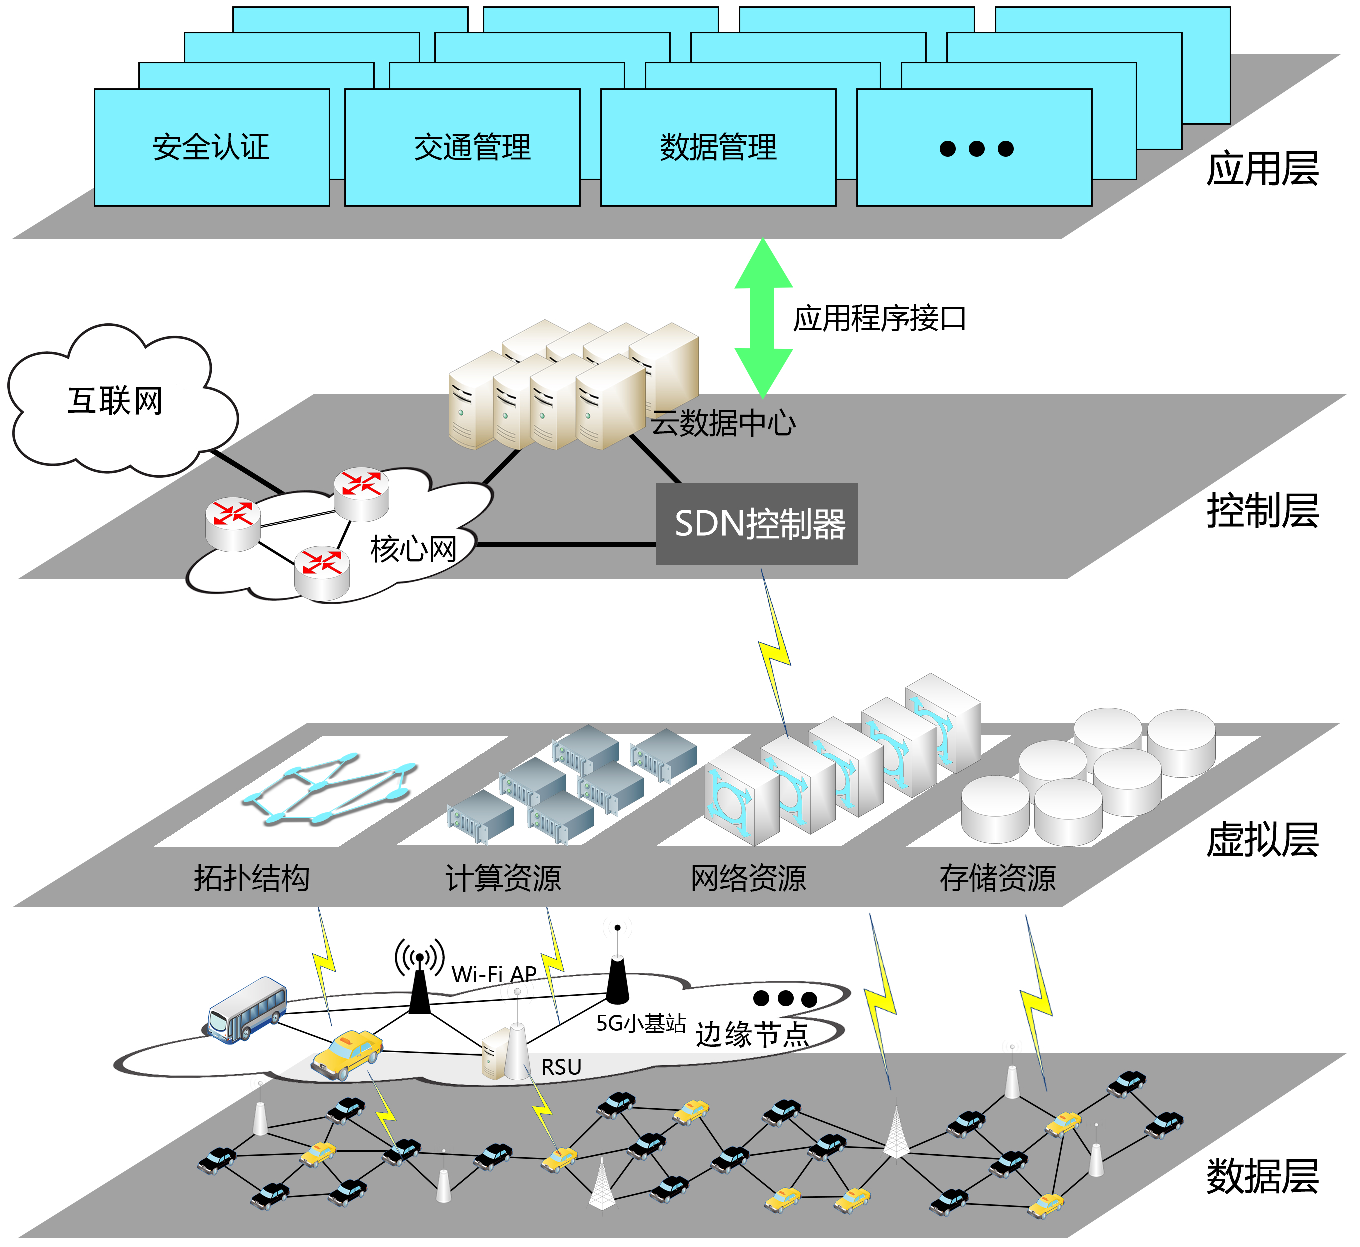
\includegraphics[width=1\columnwidth]{Fig2-1-hierarchical-architecture.pdf}
	\bicaption{异构车联网分层服务架构}{Hierarchical architecture for heterogenous vehicular networks}
	\label{fig 2-1}
\end{figure}

\subsection{基于移动边缘计算的车联网分布式服务}

本架构的数据层由如LTE基站、RSU、Wi-Fi接入点(Access Point, AP)、5G小基站和车辆等数据节点组成。除了不同的无线通信接入能力,数据节点还具备一定的计算和存储能力。其中,一些节点被抽象为边缘节点用于提供分布式服务。移动和静态的数据节点可以根据调度服务的需要被动态地分配为边缘节点。特定车辆如公交车和出租车等也可作为移动边缘节点。边缘节点不仅可以根据SDN控制器的规则执行操作,还可以为本地服务实现某些智能,进一步提高服务质量和效率。同时,边缘节点对底层资源进行一定的聚合和抽象,并向虚拟层实时更新状态,从而有助于虚拟资源的管理。因此,SDN控制器可以更方便地进行服务卸载和负载均衡的调度,从而进一步提高整个系统的性能。此外,该架构还具有良好的灵活性和可扩展性。由于边缘节点具有不同的通信接口和计算能力,因此它们可以根据实际需求进行灵活的配置和组合。此外,随着新节点的不断加入,该架构可以随时进行扩展和升级,以适应未来的需求和挑战。

\subsection{车联网中网络功能虚拟化和网络切片}

尽管网络功能虚拟化和网络切片技术在5G网络中已经被广泛研究 \cite{zhu2021wang},但是考虑到车联网中底层资源的高度异构和分布,以及上层ITS应用的高度动态和差异化服务需求等特点,将上述技术应用到车联网中仍然面临巨大挑战。因此,本章专门设计了一个虚拟层,负责抽象车联网中的计算、网络和存储资源,以在物理基础设施之上提供更高层次的抽象,使得应用程序能够更方便地访问底层资源。然而,由于网络拓扑结构的高动态性、不同的无线通信接口的差异性,以及在数据层的节点之间不断产生、感知和共享的大量信息,构建并维护底层资源的准确逻辑视图是极具挑战的。为了解决这个问题,本章将部分数据节点(如公交车、出租车、5G小基站和RSU等)抽象为边缘节点。边缘节点能够提供基于本地计算、通信和数据资源的服务,并抽象和管理可用的本地资源。一方面,边缘节点可以作为资源的管理者和协调者,负责管理和分配本地的计算、通信和存储资源,为上层应用提供优质的服务。另一方面,边缘节点还可以作为数据的处理中心,对本地产生的数据进行处理和分析,从而降低数据的传输和处理延迟。此外,由于边缘节点本身具有一定的智能,可以对诸如视频流、激光雷达点云数据等进行预处理和分析,从而进一步降低数据的传输和处理压力,提高系统的效率和可靠性。通过上述方式,不仅降低了底层资源的动态性,也减少了上层资源虚拟化的工作量。此外,该分层架构有利于NFV和NS的垂直实施。例如,给定一组具有各自QoS要求的应用,可以根据边缘的分布式调度或SDN控制器的集中式调度,以不同方式对虚拟资源进行协调。

\subsection{基于软件定义网络的逻辑集中控制}

在基于软件定义网络的车联网分层服务架构中,SDN控制器被部署在骨干网络中,并通过核心网络与云数据中心和互联网相连。与传统SDN组件类似,该控制器通过北向接口与上层应用进行通信,例如安全认证、交通管理和数据管理等。应用程序需要根据特定的需求使用相应的应用程序编程接口(Application Programming Interface, API)接口实现多维资源(例如计算、通信和存储资源)的分配、车辆行为控制、身份认证以及访问控制等功能。此外,SDN控制器通过南向接口与底层资源进行通信。需要指出的是,控制器不需要直接管理异构的物理资源。相反,通过直接使用虚拟层的资源抽象来获得虚拟资源的统一视图,从而促进SDN控制器的业务调度。虚拟层的资源抽象可以消除底层物理资源的复杂性,并为控制器提供更高的可靠性和性能。因此,通过分层架构的设计,SDN控制器不仅可以更好地管理车联网中的资源,而且可以提高车联网的可靠性和性能。为了更好地支持车联网的高度动态性和异构性,控制层还提供了一些额外的功能。例如,控制层还能够进行动态路由和流量调度,以应对车联网网络拓扑和负载的动态变化。上述功能的整合使得SDN控制器可以更好地适应车联网的复杂环境,并提供高质量的信息服务。由于SDN控制器集中控制网络资源,因此可以提高网络的安全性和可靠性。例如,控制器可以实现安全的访问控制,防止未经授权的用户访问网络资源。此外,控制器还可以实现流量监测和QoS保障,从而提高网络的可靠性和服务质量。上述服务实现的安全和可靠性的特性是车联网应用所必需的。因为上述应用涉及到交通安全和行车效率等关键问题,如果网络不稳定或者容易遭受攻击,则会对ITS应用的正常运行产生重大影响。


\section{分布式感知与异质信息融合场景}\label{section 2-3}

为了实现逻辑集中控制和支持上层 ITS 应用,分层车联网架构中的 SDN 控制器需要准确、及时地构建包含系统全局知识的逻辑视图。因此,本章首先考虑面向车载边缘计算的协作感知和异质信息融合场景,如图 \ref{fig 2-2}(a) 所示,5G 基站和路侧设备(图中$e_1$$\sim$$e_5$)可作为边缘节点提供服务。车辆能够在无线电覆盖范围内通过 V2I 通信与边缘节点进行通信,并通过搭载的车载传感器(例如激光雷达、GPS 和车载摄像头)感知异质信息。显然,车联网中的物理信息具有高度的动态性和时空相关性。同时,搭载传感器的车辆具有异质能力和有限资源,车联网通信也具有间歇性和不可靠性。因此,亟需一个量身定制的指标来定量评估由边缘节点构建的逻辑视图的质量,从而有效地衡量 VCPS 的整体性能。

\begin{figure}[h]
     \centering
     \subfloat[][]{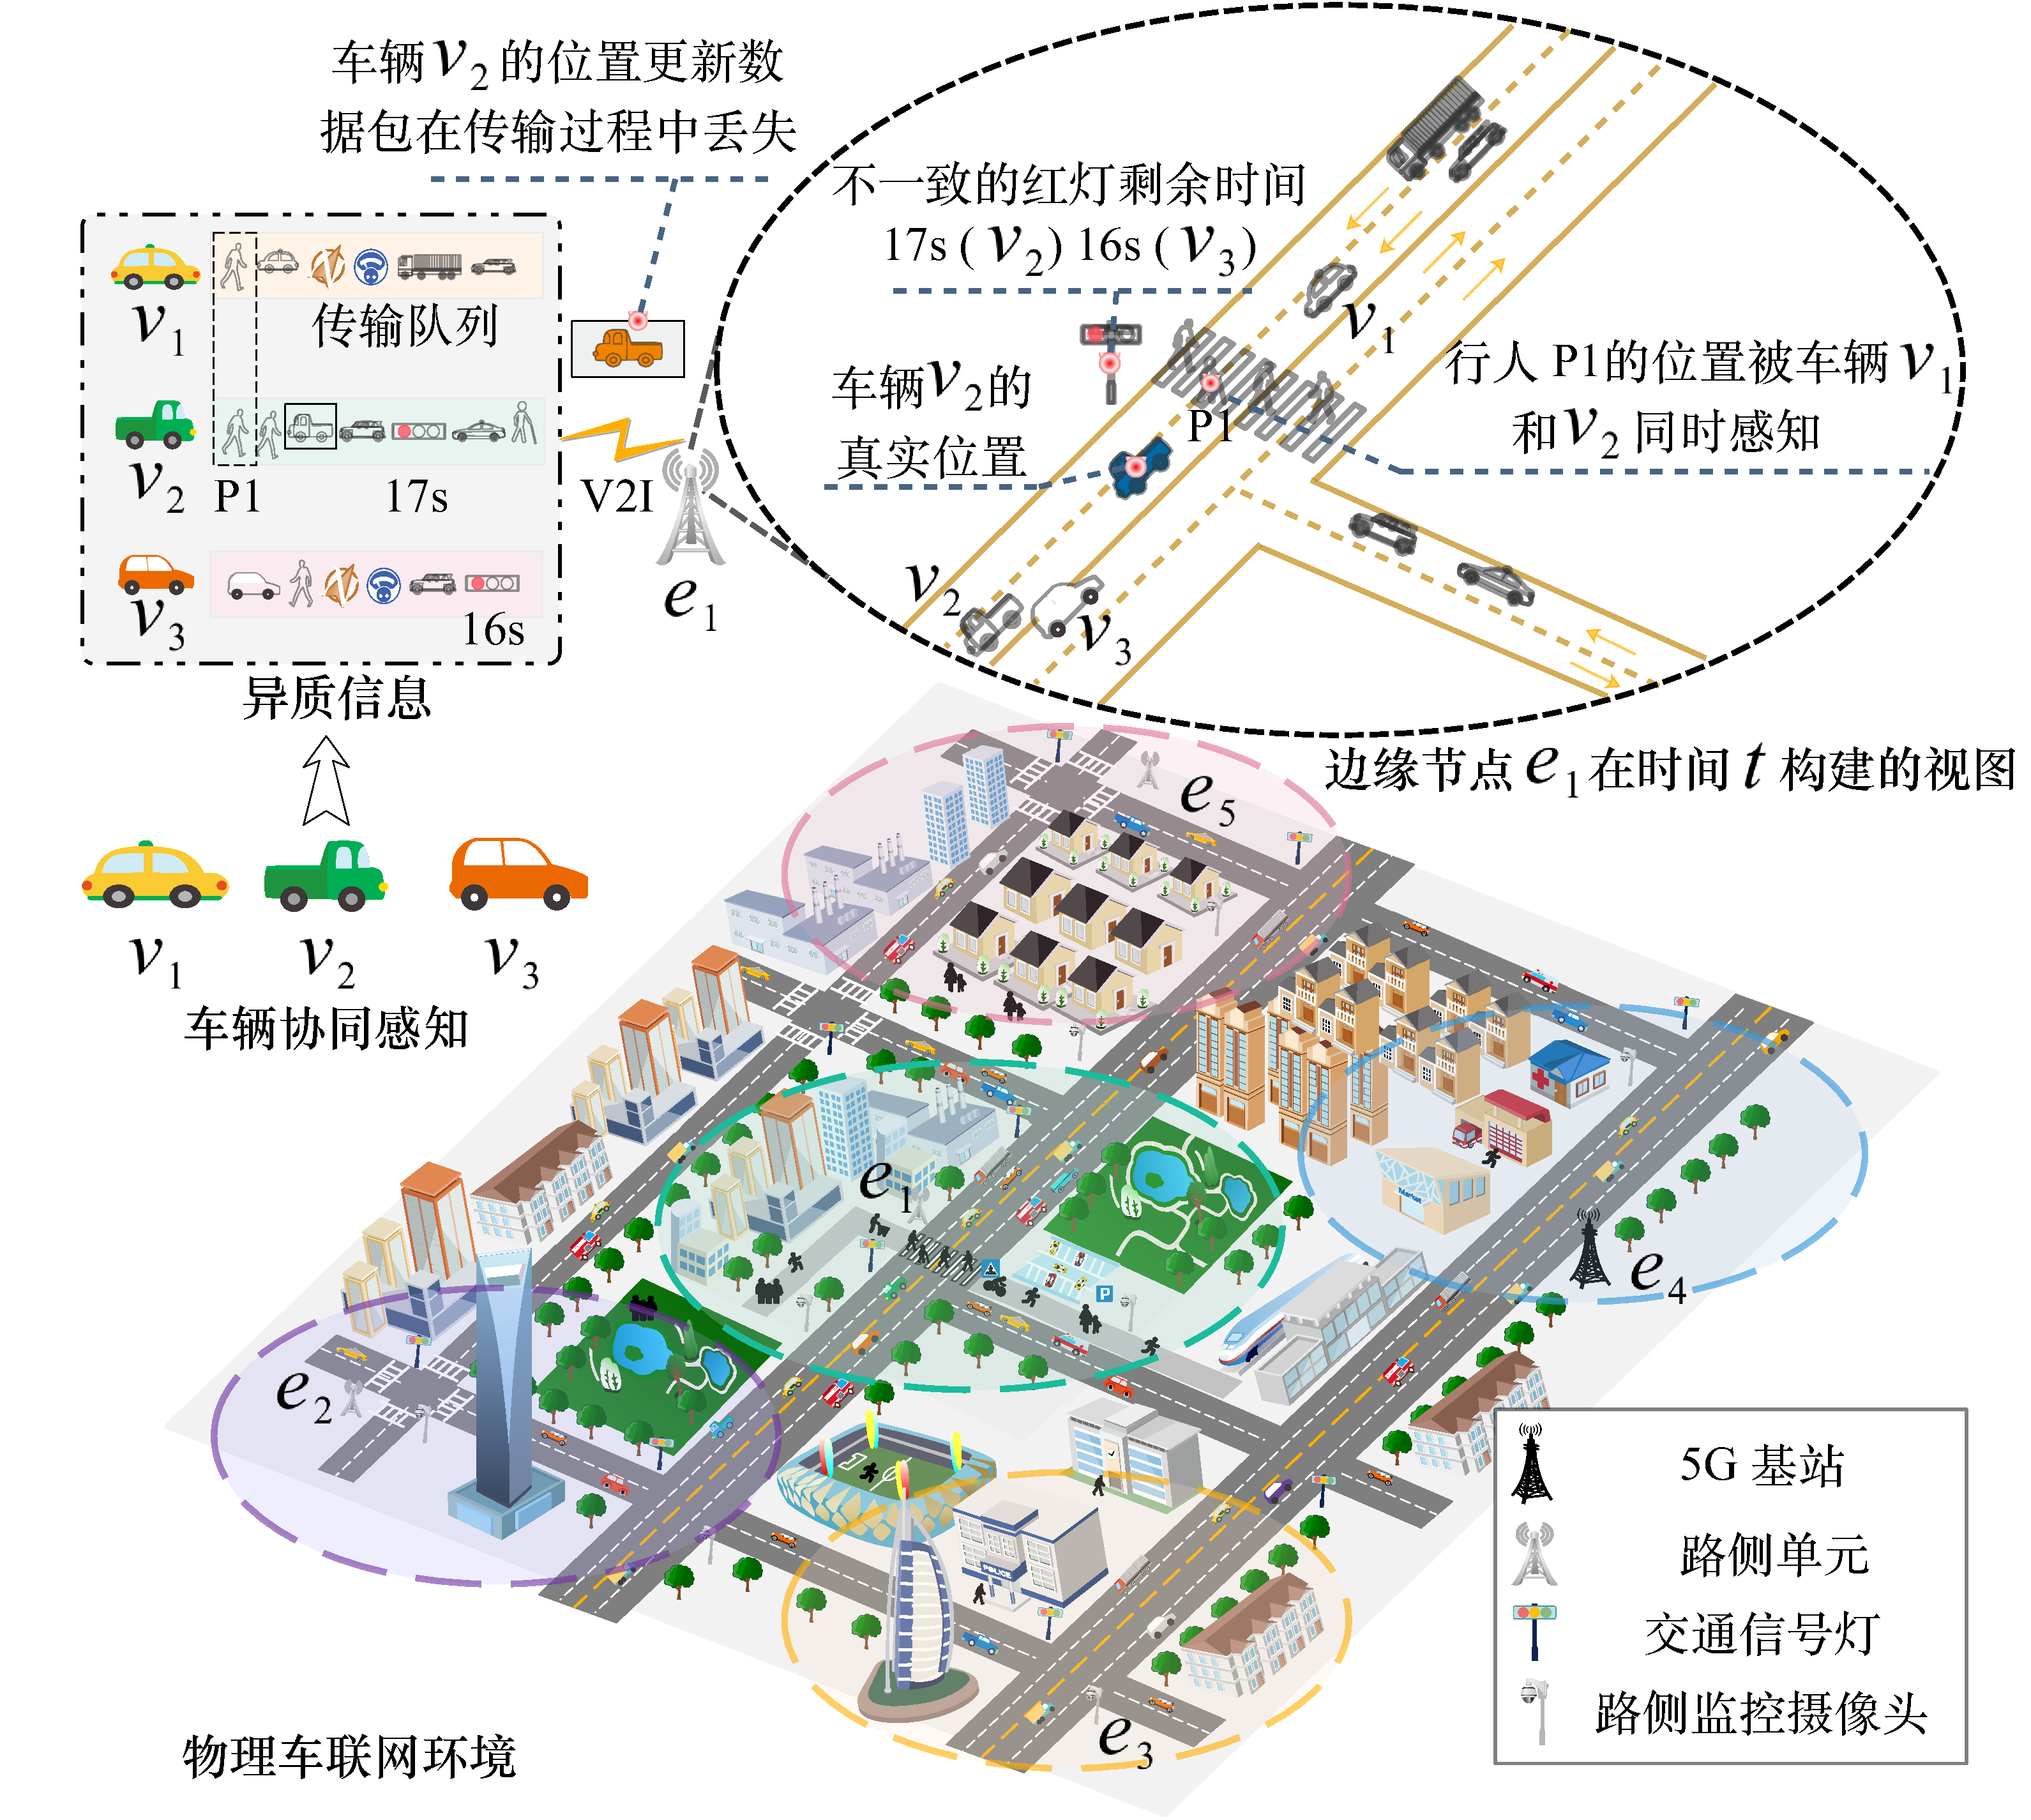
\includegraphics[width=0.7\columnwidth]{Fig2-2a-architerture.pdf}}
     \subfloat[][]{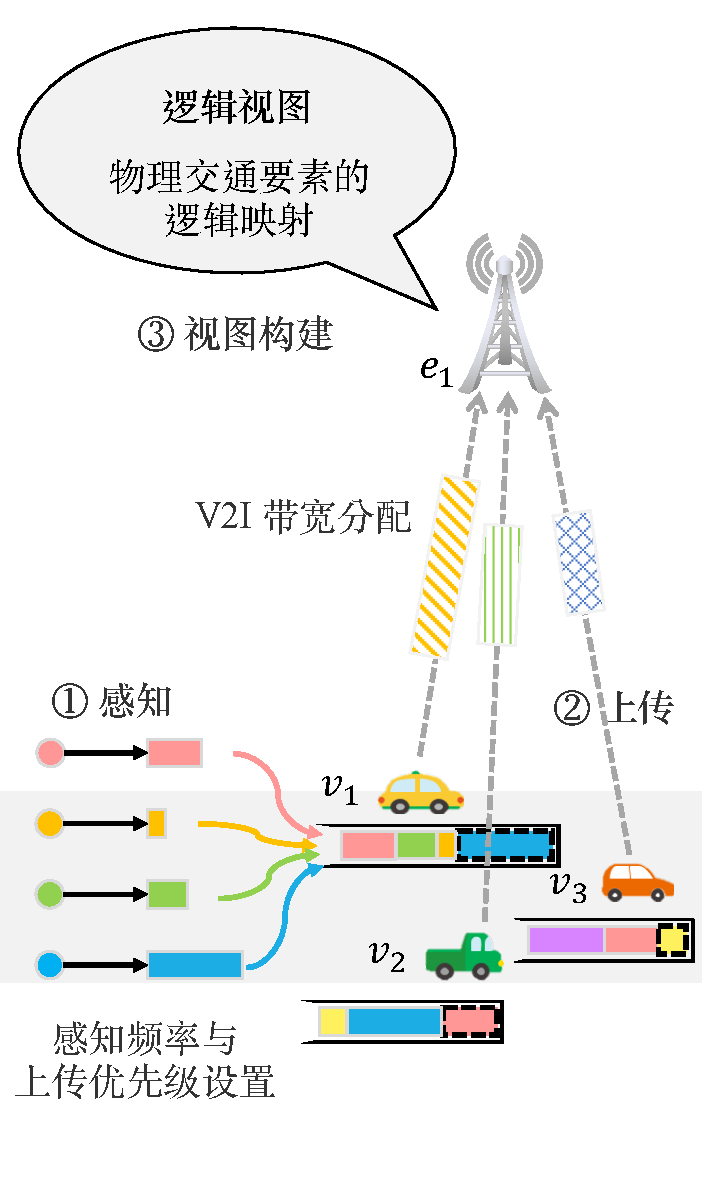
\includegraphics[width=0.3\columnwidth]{Fig2-2b-procedures.pdf}}
     \bicaption[系统场景]{系统场景。(a) 车载信息物理融合系统中分布式感知与异质信息融合 (b) 系统工作流程}[Scenario]{Scenario. (a) Distributed sensing and heterogeneous information fusion in VCPS (b) System workflow}
     \label{fig 2-2}
\end{figure}

本系统的工作流程如图\ref{fig 2-2}(b)所示,边缘节点$e_1$的逻辑视图构建包括以下三个步骤:步骤1(感知):每辆车根据其位置和感知能力感知到不同的信息。感知信息在每辆车上排队,以便上传到边缘节点。每辆车将决定这些信息的感知频率和上传优先级。由于异质信息是由车辆以不同的感知频率感知的,因此不同信息的到达时刻可能不同。同时,提高感知频率可以提高信息的新鲜度,但也会增加排队延迟。为了确定不同信息的上传优先级,必须综合考虑信息的数据量大小、V2I通信的连接性和视图需求。步骤2(上传):边缘节点将V2I带宽(即不同范围的非重叠频谱)分配给有上传任务的车辆,以便这些车辆能够同时上传他们的传感信息而不受干扰。由于边缘节点的带宽资源有限且车辆信道条件多变,分配的V2I带宽可能不足以支持及时上传数据。因此,在车辆准备上传急需的时效信息情况下,将更大的带宽分配给这些车辆,而不是分配给在更差的信道条件下的车辆(如离开V2I覆盖范围)。因此,可以通过对车辆和边缘节点之间的信噪比(Signal-to-Noise Ratio, SNR)建模来考虑了不同车辆的信道条件。同时,V2I传输速率由两个节点之间的距离和分配的带宽决定。步骤3(视图构建):边缘节点根据具体的ITS应用要求,将收到的物理信息映射到相应的逻辑元素上,从而构建逻辑视图。

此外,本章提供了一个例子来更好地说明上述观点。如图\ref{fig 2-2}(a)所示,在时间 $t$,边缘节点$e_1$构建了一个逻辑视图,并根据车辆$v_1$、$v_2$和$v_3$感知和上传的信息,在交叉路口启用了速度建议应用。一般而言,速度建议应用的目标是向正在接近交叉口的车辆提供最佳速度建议,使车辆可以顺利通过,从而达到最大化整体交通效率。假设车辆$v_2$和$v_3$都能感知交通灯信息,但感知的红灯剩余时间数值不一致,进一步导致信息不一致。同时,同一物理要素的状态可能会被多辆车同时感知到。在这种情况下,该消息只需要由其中一辆车在一定时间内上传以节省V2I带宽。只要物理要素在边缘节点以相同的质量水平建模,其就可以被应用于不同的应用,而不需要由不同的车辆重复上传。此外,数据包丢失可能导致物理车联网环境和视图之间的差距。例如,假设车辆$v_2$的位置更新数据包丢失,这会导致其真实位置与时间$t$视图上的位置之间存在明显的不一致。因此,定量评估边缘节点构建的视图的质量,并为协作感知和信息融合设计有效的调度机制,以最大限度地提高VCPS的整体质量是至关重要且具有挑战性的。

\section{车载信息物理融合质量指标设计}\label{section 2-4}

\subsection{基本符号}

系统的离散时间片集合用$\mathbf{T}=\{1, \ldots, t, \ldots, T\}$表示。
异质信息的集合用$\mathbf{D}=\{1, \ldots, d, \ldots, D\}$表示,其中信息$d$可以用一个双元组$d=\left(\operatorname{type}_d, \left|d\right| \right)$表示,其中$\operatorname{type}_d$为类型,$\left|d\right|$为数据量。
车辆的集合用$\mathbf{V}=\{1, \ldots, v, \ldots, V\}$表示,其中车辆$v$的特征用一个三元组$v=\left (l_v^t, \mathbf{D}_v, \pi_v \right )$表示,其中$l_v^t$是车辆$v$在时间$t$的位置;$\mathbf{D}_v$是车辆$v$可以感知的信息集合,$\pi_v$是车辆$v$的传输功率。
边缘节点的集合用$\mathbf{E}=\{1, \ldots, e, \ldots, E\}$表示,其中边缘节点$e$的特征用一个三元组$e=\left (l_e, g_e, b_e \right)$表示,其中$l_e$是位置,$g_e$是通信范围,$b_e$是带宽。
在时间$t$,车辆$v$与边缘节点$e$的距离表示为$\operatorname{dis}_{v,e}^t \triangleq \operatorname{distance} \left (l_v^t, l_e \right )$,其中$\operatorname{distance}\left(\cdot,\cdot\right)$是欧氏距离。

车辆$v$在时间$t$所感知的信息集合用$\mathbf{D}_v^t\subseteq \mathbf{D}_v$表示。
对于车辆在时间$t$感知到的信息类型,需要各不相同,即对于$\mathbf{D}_v^t$中的任意信息$d$,信息类型都是不同的,$\operatorname{type}_{d^*} \neq \operatorname{type}_{d}, \forall d^* \in \mathbf{D}_v^t \setminus \left\{ d\right \}, \forall d \in \mathbf{D}_v^t$。
车辆$v$在时间$t$对于信息$d$的感知频率用$\lambda_{d,v}^t$表示。
由于感知能力有限,车辆感知频率需满足$\lambda_{d,v}^{t} \in [\lambda_{d,v}^{\min} , \lambda_{d,v}^{\max} ], \forall d \in \mathbf{D}_v^t, \forall v \in \mathbf{V}, \forall t \in \mathbf{T}$, 其中 $\lambda_{d,v}^{\min}$ 和 $\lambda_{d,v}^{\max}$ 分别为车辆$v$对于类型为$\operatorname{type}_{d}$的信息的最低和最高感知频率。
车辆$v$中的信息$d$在时间$t$的上传优先级用$p_{d,v}^t$表示,且${p}_{d^*, v}^t \neq {p}_{d, v}^t, \forall d^* \in \mathbf{D}_v^t \setminus \left\{ d\right \}, \forall d \in \mathbf{D}_v^t, \forall v \in \mathbf{V}, \forall t \in \mathbf{T}$。
在时间$t$内处于边缘节点$e$的无线电覆盖范围内的车辆集合表示为$\mathbf{V}_e^t=\left \{v \vert \operatorname{dis}_{v,e}^t \leq g_e, \forall v \in \mathbf{V} \right \}, \mathbf{V}_e^t \subseteq \mathbf{V}, \forall e \in \mathbf{E}$。
边缘节点$e$在时间$t$为车辆$v$分配的V2I带宽用$b_{v, e}^t$表示,且$b_{v, e}^t \in \left [0,b_e \right], \forall v \in \mathbf{V}_e^{t}, \forall e \in \mathbf{E}, \forall t \in \mathbf{T}$。
边缘节点$e$分配的V2I带宽总和不能超过其带宽容量$b_e$,即${\sum_{\forall v \in \mathbf{V}_e^{t}}b_{v, e}^t} \leq b_e, \forall e \in \mathbf{E}, \forall t \in \mathbf{T}$。

\subsection{系统模型}
本系统分布式感知模型如图\ref{fig 2-3}所示。
车辆感知的信息到达间时间和排队时间通过多类M/G/1优先级队列(Multi-Class M/G/1 Priority Queue)\cite{qian2020minimizing}对车辆中的感知信息队列进行建模得到。
假定车辆$v$中具有相同类型$\operatorname{type}_d$的信息传输时间分布在每个时间片内保持稳定。
类型为$\operatorname{type}_d$的信息传输时间$\operatorname{\hat{g}}_{d, v, e}^t$遵循一类一般分布(General Distribution),其均值为$\alpha_{d, v}^t$,二阶矩和三阶矩分别为$\beta_{d, v}^t$和$\gamma_{d, v}^t$,那么该分布集合可以表示为:
\begin{align}
	\mathbb{P}=\left\{\hat{\mathrm{g}}_{d, v, e}^t:\right. & \mathbb{E}\left[\hat{\mathrm{g}}_{d, v, e}^t\right]=\alpha_{d, v}^t, \notag \\
	& \mathbb{E}\left[\hat{\mathrm{g}}_{d, v, e}^t-\alpha_{d, v}^t\right]^2=\beta_{d, v}^t \notag \\
	& \mathbb{E}\left[\operatorname{\hat{g}}_{d, v, e}^t-\alpha_{d, v}^t\right]^{3}=\left.\gamma_{d, v}^t \right\}
\end{align}
因此,上传负载 $\rho_{v}^{t}$ 可表示为:
\begin{equation}
    \rho_{v}^{t}=\sum_{\forall d \subseteq \mathbf{D}_v^t} \lambda_{d,v}^{t}  \alpha_{d, v}^t
\end{equation}

\begin{figure}[h]
\centering
  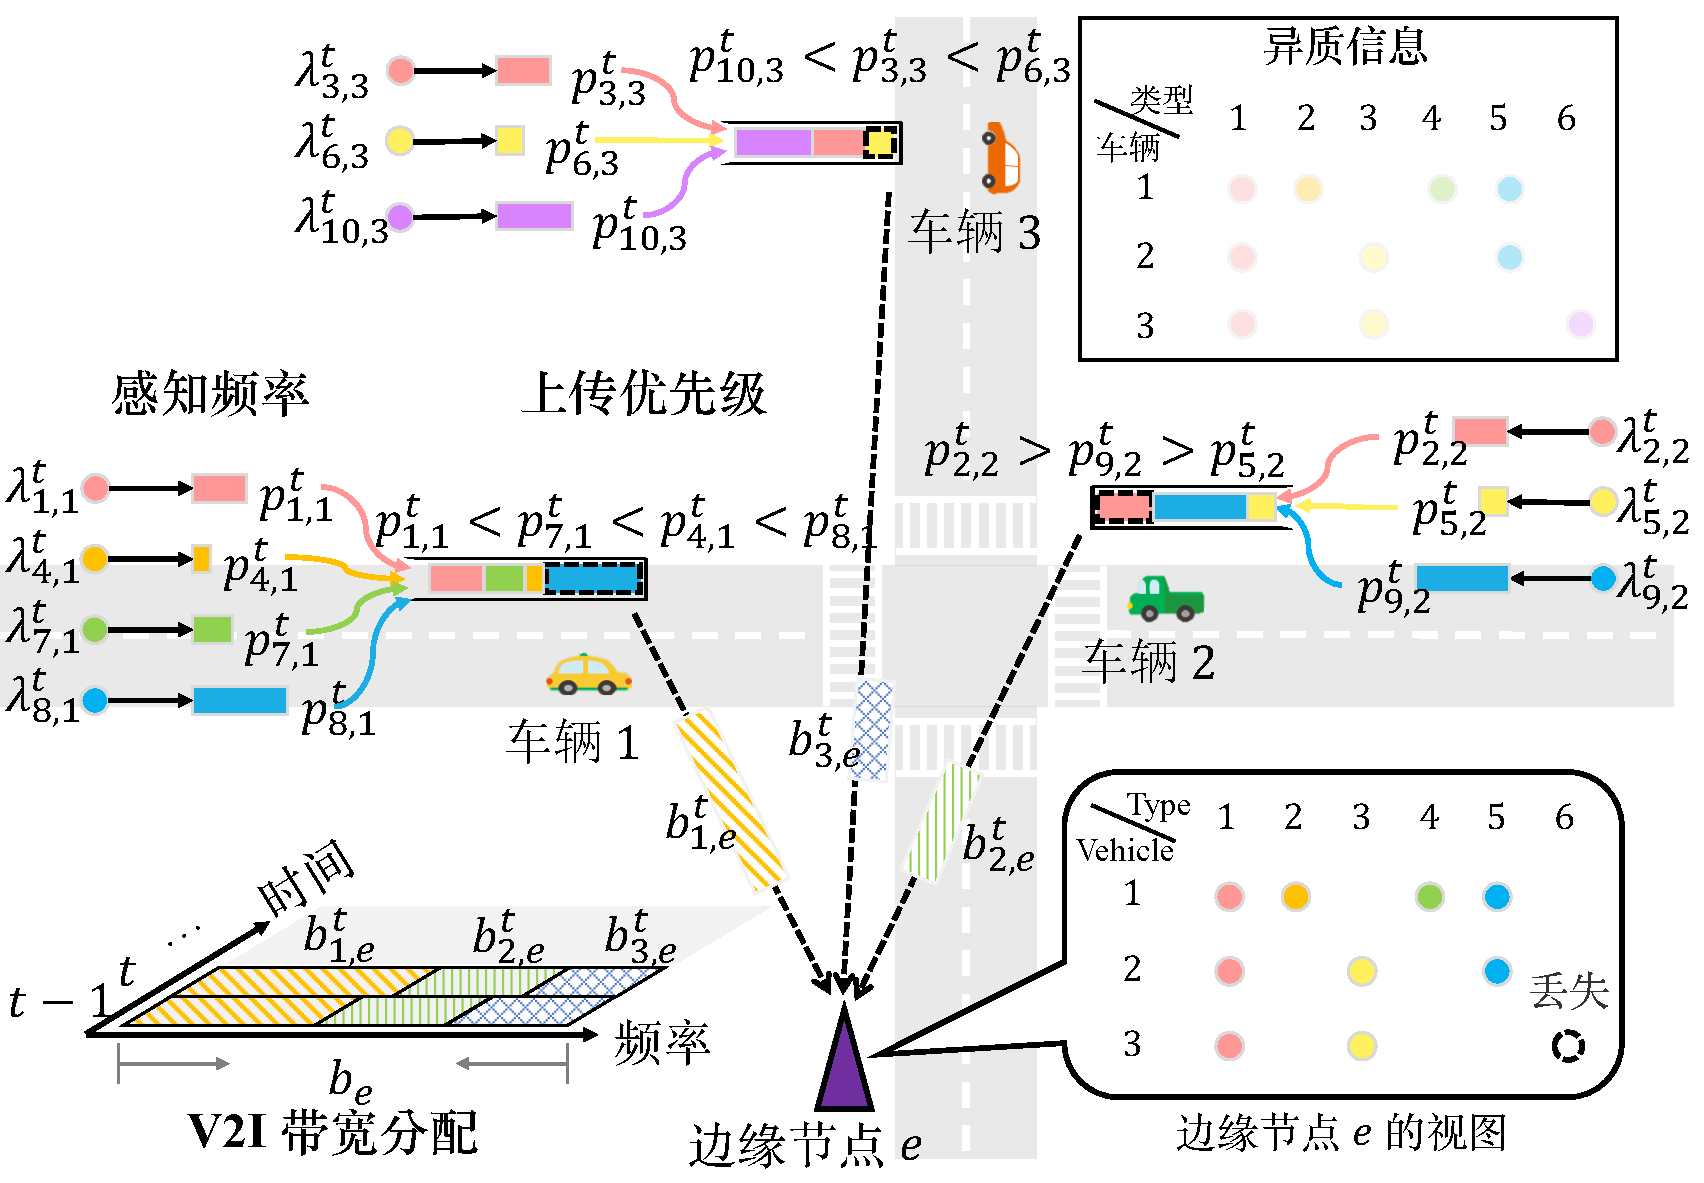
\includegraphics[width=0.8\columnwidth]{Fig2-3-cooperative-sensing.pdf}
  \bicaption{分布式感知模型}{Distributed sensing model}
  \label{fig 2-3}
\end{figure}

为了确保队列具有稳定状态,需要满足 $\rho_{v}^{t} < 1$。
到达间隔时间$\operatorname{a}_{d, v}^t$是指车辆$v$中两个相邻的具有相同类型$\operatorname{type}_d$的信息到达时间差,其计算公式为:
\begin{equation}
    \operatorname{a}_{d, v}^t=\frac{1}{\lambda_{d, v}^{t}}
\end{equation}
在时间$t$内,车辆$v$中具有比信息$d$更高上传优先级的信息集合可表示为:
\begin{equation}
\mathbf{D}_{d, v}^t=\left\{d^* \mid p_{d^*, v}^t>p_{d, v}^t, \forall d^* \in \mathbf{D}_v^t\right\} 
\end{equation}
其中$p_{d^*, v}$是信息$d^* \in \mathbf{D}_v^t$的上传优先级。
  因此,信息$d$前面的上传负载(车辆$v$在时间$t$内要在$d$前面上传的数据量)表示为:
\begin{equation}
\rho_{d, v}^t=\sum_{\forall d^* \in \mathbf{D}_{d, v}^t} \lambda_{d^*, v}^t \alpha_{d^*, v}^t
\end{equation}
其中$\lambda_{d^*, v}^t$和$\alpha_{d^*, v}^t$分别是时间$t$内车辆$v$中信息$d^*$的感知频率和平均传输时间。
车辆$v$中类型为$\operatorname{type}_d$的信息的排队时间用$\operatorname{q}_{d, v}^t$表示。
根据Pollaczek$-$Khintchine公式\cite{takine2001queue},平均排队时间$\operatorname{\bar{q}}_{d, v}^t$计算如下:
\begin{equation}
    \operatorname{\bar{q}}_{d, v}^t= \frac{1} {1 - \rho_{d, v}^{t}} 
        \left[ \alpha_{d, v}^t + \frac{ \lambda_{d, v}^{t} \beta_{d, v}^t + \sum\limits_{\forall d^* \in \mathbf{D}_{d, v}^t} \lambda_{d^*,s}^t \beta_{d^*, v}^t }{2\left(1-\rho_{d, v}^{t} - \lambda_{d, v}^{t}  \alpha_{d, v}^t\right)}\right] 
        - \alpha_{d, v}^t
\label{equ 2-6}
\end{equation}
进一步,多类M/G/1优先队列中排队时延的上界分析见附录\ref{appendix e}。

本章根据香农理论对通过V2I通信的数据上传进行建模。
在时间$t$,车辆$v$和边缘节点$e$的V2I通信的信噪比用$\operatorname{SNR}_{v, e}^{t}$表示,其计算方法如公式\ref{equ 2-7}\cite{sadek2009distributed}所示。
\begin{equation}
    \label{equ 2-7}
    \operatorname{SNR}_{v, e}^{t}=\frac{1}{N_{0}}  \left|h_{v, e}\right|^{2} \zeta  {\operatorname{dis}_{v, e}^{t}}^{-\varphi} {\pi}_v
\end{equation}
其中$N_{0}$为加性白高斯噪声(Additive White Gaussian Noise, AWGN);$h_{s, e}$为信道衰减增益;$\zeta$为取决于天线设计的常数;$\varphi$为路径损耗指数。
车辆$v$和边缘节点$e$之间在时间$t$的V2I传输率用$\operatorname{z}_{v, e}^t$表示,其计算如下: 
\begin{equation}
    \operatorname{z}_{v, e}^t=b_{v, e}^{t} \log _{2}\left(1+\mathrm{SNR}_{v, e}^{t}\right)
    \label{equ 2-8}
\end{equation}
其中$b_{v, e}^{t}$是分配给车辆$v$在时间$t$的带宽。
值得注意的是,给定车辆$v$的传输功率$\pi_s$,车辆$v$和边缘节点$e$之间在时间$t$的V2I通信的信噪比可以通过公式\ref{equ 2-7}得到,进一步可由公式\ref{equ 2-8}得到传输速率。
因此,信息$d$从车辆$v$到边缘节点$e$的传输时间用$\mathrm{w}_{d, v, e}^t$表示,其计算公式为:
\begin{equation}
	\mathrm{w}_{d, v, e}^t=\frac{\left|d\right|}{\operatorname{z}_{v, e}^t}
\end{equation}
成功传输需要在数据包传输过程中,接收到的信噪比高于某个阈值,其被称为 SNR Wall \cite{tandra2008snr},该阈值通过以下方式获得:
\begin{equation}
\mathrm{SNR}_{\text {wall }}=\frac{\sigma^{2}-1}{\sigma}
\end{equation}
其中$\sigma=10^{\nu / 10}$,$\nu$是以dB衡量的参数,量化了噪声不确定性的大小。
\begin{equation}
	\left(\nu^2 - 1\right) {N_0}={\pi_v} \nu
\end{equation}
因此,表示信息$d$是否从车辆$v$成功传输到边缘节点$e$的成功传输指示器表示为:
\begin{numcases}{\operatorname{c}_{d, v, e}^t=}
1, \forall {t^{*}} \in\left[t + \operatorname{\bar{q}}_{d, v}^t, t + \operatorname{\bar{q}}_{d, v}^t + \operatorname{w}_{d, v, e}^t\right], \operatorname{SNR}_{v, e}^{t^{*}}>\mathrm{SNR}_{\text {wall }} \notag \\
0, \exists {t^{*}} \in\left[t + \operatorname{\bar{q}}_{d, v}^t, t + \operatorname{\bar{q}}_{d, v}^t + \operatorname{w}_{d, v, e}^t\right], \operatorname{SNR}_{v, e}^{t^{*}} \leq \mathrm{SNR}_{\text {wall }}
\end{numcases}
由车辆$v$传输并由边缘节点$e$接收的信息集合表示为 $\mathbf{D}_{v, e}^t = \{ d \mid \operatorname{c}_{d, v, e}^t = 1, \forall d \in \mathbf{D}_v \}, \mathbf{D}_{v, e}^t \subseteq \mathbf{D}_v^t, \forall v \in \mathbf{V}, \forall e \in \mathbf{E}$。

\subsection{Age of View}
系统中的视图集合用$\mathbf{I}$表示,视图$i \in \mathbf{I}$所需的信息集用$\mathbf{D}_{i}$表示,它是特定ITS应用所需的物理交通元素的映射,它表示为:
\begin{equation}
	\mathbf{D}_{i} = \{d \mid y_{d, i} = 1, \forall d \in \mathbf{D} \}
\end{equation}
视图$i$所需元素的数量用$|\mathbf{D}_{i}|$表示。
边缘节点$e$在时间$t$所需的视图集合用$\mathbf{I}_e^t \subseteq \mathbf{I}$表示。
因此,边缘节点$e$收到的并被视图$i$需要的信息集用下式表示:
\begin{equation}
    \mathbf{D}_{i, e}=\bigcup_{\forall i \in \mathbf{I}}\left(\mathbf{D}_i \cap \mathbf{D}_{v, e}^t\right), \forall v \in \mathbf{V}_e^t, \forall e \in \mathbf{E}
\end{equation}
且$| \mathbf{D}_{i, e} |$是边缘节点$e$收到并被视图$i$需要的信息数量。
接下来,定义异质信息融合的三个特征,包括视图的时效性、完整性和一致性。

首先,异质信息是随时间变化的,信息的新鲜度对于视图质量至关重要。
因此,车辆$v$中的信息$d$的时效性定义如下:
\begin{definition}
	车辆$v$的信息$d$的时效性 $\xi_{d,v} \in (0, +\infty)$被定义为信息$d$的间隔到达时间、排队时间和传输时间之和。
	\begin{equation}
    	\xi_{d, v} = \operatorname{a}_{d, v}^t + \operatorname{q}_{d, v}^t + \operatorname{w}_{d, v, e}^t, \forall d \in \mathbf{D}_v^t, \forall v \in \mathbf{V}
	\end{equation}
\end{definition}
\noindent 其中 $\operatorname{a}_{d, v}^t$、$\operatorname{q}_{d, v}^t$ 和 $\operatorname{w}_{d, v, e}^t$ 分别为信息$d$的间隔到达时间、排队时间和传输时间。
进一步,视图的时效性定义如下:
\begin{definition}
视图$i$的时效性 $\Xi_{i} \in (0,+\infty)$被定义为信息时效性总和。
	\begin{equation}
    	\Xi_{i} = \sum_{\forall v \in \mathbf{V}} \sum_{\forall d \in \mathbf{D}_{i, e} \cap \mathbf{D}_v^t } \xi_{d, v}, \forall i \in \mathbf{I}_e^t, \forall e \in \mathbf{E}
	\end{equation}
\end{definition}

其次,车联网具有包括车辆高移动性、网络资源有限性和无线通信不可靠的固有特性。
由于车辆和边缘节点之间的无线传输连接断开,或者传输过程中数据包的丢失,视图可能是不完整的。
因此,视图的完整性定义如下:
\begin{definition}
	视图$i$的完整性$\Phi_{i} \in [0,1]$被定义为边缘节点$e$实际收到的信息数量与所需总量之比。
	\begin{equation}
	\Phi_{i}= {| \mathbf{D}_{i, e} |} \big/ {|D_{i} |}, \forall i \in \mathbf{I}_e^t, \forall e \in \mathbf{E}
	\end{equation}
\end{definition}
\noindent 其中$|\mathbf{D}_{i, e}|$是边缘节点$e$收到并被视图$i$需要的信息数量,$|\mathbf{D}_{i}|$是视图$i$需要的信息总数量。

再次,由于不同类型的信息有各自的感知频率和上传优先级,在构建视图时,需要使不同类型信息的版本尽可能接近。
因此,视图的一致性定义如下: 
\begin{definition}
视图$i$的一致性$\Psi_{i} \in (0,+\infty)$被定义为信息接收时间与视图所需信息的平均接收时间之差的二次方和。
\begin{equation}
\Psi_{i}=\sum_{\forall v \in \mathbf{V}} \sum_{\forall d \in \mathbf{D}_{i, e} \cap \mathbf{D}_v^t} \left|\operatorname{q}_{d, v}^t + \operatorname{w}_{d, v, e}^t - \psi_{i} \right|^{2}, \forall i \in \mathbf{I}_e^t, \forall e \in \mathbf{E}
\end{equation}
\end{definition}
\noindent 其中 $\psi_{i}$ 是视图$i$所需信息的平均接收时间,其可由下式得到:
\begin{equation}
	\psi_{i} = \frac{1}{|D_{i, e}|} {\sum_{\forall v \in \mathbf{V}}\sum_{\forall d \in D_{i, e} \cap \mathbf{D}_v^t} \left( \operatorname{q}_{d, v}^t + \operatorname{w}_{d, v, e}^t\right) }, \forall i \in\mathbf{I}_e^t, \forall e \in \mathbf{E}
\end{equation}

最后,本章给出了Age of View的正式定义,其综合了视图的时效性、完整性和一致性。
\begin{definition}
Age of View $\operatorname{AoV}_{i} \in (0, 1)$ 被定义为视图$i$的归一化时效性、完整性和一致性的加权平均值。
	\begin{equation}
	    \operatorname{AoV}_{i} = w_1  \hat{\Xi}_{i} + w_2  \hat{\Phi}_{i}+  w_3 \hat{\Psi}_{i}, \forall i \in \mathbf{I}_e^t, \forall e \in \mathbf{E}
\end{equation}
\end{definition}
\noindent 其中,$\hat{\Xi}_{i} \in (0, 1)$、$\hat{\Phi}_{i} \in (0, 1)$和$\hat{\Psi}_{i} \in (0, 1)$分别表示视图$i$的归一化时效性、归一化完整性和归一化一致性。
$\operatorname{AoV}_{i}$的值越低,说明构建的视图质量越高。
需要注意的是,由于视图的时效性、完整性和一致性的维度不同,为了形成AoV的统一表示,将它们归一化到$(0,1)$范围内,具体如下:
\begin{numcases}{}
\hat{\Xi}_{i} = {\Xi}_{i} \big/ \left( \delta_\xi | \mathbf{D}_{v, e} |   T \right) \notag \\ 
\hat{\Phi}_{i} = 1 - {\Phi}_{i}  \notag \\
\hat{\Psi}_{i} = {\Psi}_{i} \big/ \left( \delta_\psi  \max\limits_{\substack{\forall d \in \mathbf{D}_v \cap \mathbf{D}_v^t \\ \forall v \in \mathbf{V}}}{\left\{ \left|\operatorname{q}_{d, v}^t + \operatorname{g}_{d, v, e}^t - \psi_{i} \right|^{2}\right\}}   \right)
\end{numcases}
\noindent 其中$\delta_{\xi} \in(0,1)$和$\delta_\psi \in(0,1)$分别是时效性和一致性的数据比例系数,通过缩减时效性和一致性的理论最大值避免归一化结果将大部分数值集中在一个小范围内。
$\hat{\Xi}_{i}$、$\hat{\Phi}_{i}$和$\hat{\Psi}_{i}$的加权系数分别用$w_1$、$w_2$和$w_3$表示,且$w_1+w_2+w_3=1$。
加权系数可以根据ITS应用的不同要求进行相应的调整。
例如,对于道路交叉口的速度咨询应用,车辆需要从边缘节点接收实时速度的指令,以便安全顺利地通过交叉口。
在这种情况下,时效性因素(例如,实时交通灯状态)与完整性因素(例如,行人在视图中被建模)相比,在视图建模中更为重要。

\subsection{问题定义}
鉴于上述指标AoV是单独评估视图的质量,本章进一步在系统层面上定义VCPS的质量如下:
\begin{definition}
VCPS的质量$\Upsilon \in (0,1)$被定义为在调度期$\mathbf{T}$中边缘节点的每个视图$i$的AoV的补集平均值。
\begin{equation}
\Upsilon=\frac{\sum_{\forall t \in \mathbf{T}} \sum_{\forall e \in \mathbf{E}} \sum_{\forall i \in \mathbf{I}_e^t} \left(1 - \operatorname{AoV}_{i}\right)}{\sum_{\forall t \in \mathbf{T}} \sum_{\forall e \in \mathbf{E}} |\mathbf{I}_e^t| }
\end{equation}
\end{definition}

给定一个确定性的解决方案$(\bf\Lambda, \mathbf{P}, \mathbf{B} )$,其中$\bf\Lambda$表示确定的感知频率,$\mathbf{P}$表示确定的上传优先级,$\mathbf{B}$表示确定的V2I带宽分配,它们分别表示为:
\begin{numcases}{}
{\bf\Lambda} = \left\{ \lambda_{d, v}^{t} \vert \forall d \in \mathbf{D}_v^t  , \forall v \in \mathbf{V}, \forall t \in \mathbf{T} \right\} \notag \\ 
\mathbf{P} = \left \{ p_{d, v}^{t} \vert \forall d \in \mathbf{D}_v^t  , \forall v \in \mathbf{V}, \forall t \in \mathbf{T}\right \} \notag \\
\mathbf{B} = \left \{ b_{v, e}^t \vert \forall v \in \mathbf{V}_e^t, \forall e \in \mathbf{E}, \forall t \in \mathbf{T}\right \}
\end{numcases}
\noindent 其中,$\lambda_{d,v}^{t}$ 表示车辆$v$在时间$t$对信息$d$的感知频率,$p_{d, v}^{t}$ 表示车辆$v$在时间$t$对信息$d$的上传优先级,$b_{v, e}^t$ 表示边缘节点$e$在时间$t$为车辆$v$分配的V2I 带宽。

本章旨在通过车辆间分布式感知与边缘节点的异质信息融合以构建边缘视图并进一步实现高质量车载信息物理融合。
本章的目标问题是通过确定所有车辆上不同信息感知频率、上传优先级,以及边缘节点对于通信覆盖范围内所有车辆进行V2I带宽分配,以最大限度地提高VCPS的质量。
因此,最大化VCPS质量问题形式化定义如下:
\begin{align}
	&\max_{\bf\Lambda, \mathbf{P}, \mathbf{B}} \Upsilon \notag \\
	\text { s.t. }
    \mathcal{C}2.1: & \lambda_{d,v}^{t} \in \left [\lambda_{d,v}^{\min} , \lambda_{d,v}^{\max} \right ], \forall d \in \mathbf{D}_v^t , \forall v \in \mathbf{V}, \forall t \in \mathbf{T} \notag \\
     \mathcal{C}2.2: &{p}_{d^*, v}^t \neq {p}_{d, v}^t, \forall d^* \in \mathbf{D}_v^t \setminus \left\{ d\right \}, \forall d \in \mathbf{D}_v^t, \forall v \in \mathbf{V}, \forall t \in \mathbf{T} \notag \\
    \mathcal{C}2.3: & b_{v, e}^t \in \left[ 0 , b_e \right ], \forall v \in \mathbf{V}_e^t, \forall e \in \mathbf{E}, \forall t \in \mathbf{T} \notag \\
    \mathcal{C}2.4: & \sum_{\forall d \subseteq \mathbf{D}_v^t} \lambda_{d,v}^{t}  \alpha_{d, v}^t < 1,\ \forall v \in \mathbf{V}, \forall t \in \mathbf{T}  \notag \\
    \mathcal{C}2.5: & {\sum_{\forall v \in \mathbf{V}_e^{t}}b_{v, e}^t} \leq b_e, \forall e \in \mathbf{E}, \forall t \in \mathbf{T}
\end{align}
约束条件$\mathcal{C}2.1$要求车辆$v$中的信息$d$在时间$t$的感知频率应满足其感知能力的要求。
$\mathcal{C}2.2$ 保证时间$t$内车辆$v$中信息$d$的上传优先级。
$\mathcal{C}2.3$ 规定边缘节点$e$在时间$t$为车辆$v$分配的V2I带宽不能超过其带宽容量$b_e$。
$\mathcal{C}2.4$保证在调度周期$\mathbf{T}$内队列稳定状态。
$\mathcal{C}2.5$要求边缘节点$e$分配的V2I带宽之和不能超过其容量$b_e$。

\section{基于差分奖励的多智能体强化学习算法设计}\label{section 2-5}

\subsection{算法模型}
本章将详细介绍所提基于差分奖励的多智能体深度强化学习算法,其模型如图\ref{fig 2-4}所示,由$V$辆车、边缘节点$e$、VCPS环境和经验回放缓存组成。
首先,车辆$v$决定其动作$\boldsymbol{a}_{v}^{t}$,包括确定感知频率和上传优先级。
特别地,车辆$v$动作由行动者网络生成,其输入是对系统状态的局部观测$\boldsymbol{o}_{v}^{t}$。
车辆$v$的评论家网络评估由相应行动者网络产生的动作。
其次,边缘节点$e$根据车辆预测轨迹和视图需求决定其动作$\boldsymbol{a}_{e}^{t}$,即为通信覆盖范围内的车辆分配V2I带宽。
再次,环境根据动作$\{ \boldsymbol{a}_{1}^{t}, \ldots, \boldsymbol{a}_{v}^{t}, \ldots, \boldsymbol{a}_{V}^{t}, \boldsymbol{a}_{e}^{t}\}$ 获得系统奖励,即边缘节点$e$在时间$t$实现的VCPS质量。
并采用基于差分奖励\cite{foerster2018counterfactual}的信用分配,将系统奖励分为差分奖励$\{r_1^t, \ldots, r_{V}^t\}$,其中$r_v^t$被用来评估车辆$v$对视图构建的贡献。
最后,相关的交互经验包括当前系统状态、车辆动作、差分奖励和下一时刻系统状态,都存储在经验回放缓存中,并用来训练车辆的行动者和评论家网络。
算法模型的主要组成部分设计如下:

1) \textbf{系统状态}: 边缘节点定期广播其视图需求和缓存信息。在时间$t$内,车辆$v$的系统状态的本地观测被表示为:
	\begin{equation}
		\boldsymbol{o}_{v}^{t}=\left\{\mathbf{D}_{v}^{t}, \mathbf{D}_{e}^{t}, \mathbf{I}_e^t\right\}
	\end{equation} 
	\noindent 其中$\mathbf{D}_{v}^{t}$表示车辆$v$在时间$t$感知的信息集合;
	$\mathbf{D}_{e}^{t}$ 表示在时间$t$边缘节点$e$中的缓存信息集合,
	以及$\mathbf{I}_e^t$表示边缘节点$e$在时间$t$的边缘节点所需的视图集合。
	那么,时间$t$的系统状态可表示为:
	\begin{equation}
		\boldsymbol{o}^{t}=\left\{\mathbf{D}_{1}^{t}, \ldots, \mathbf{D}_{v}^{t}, \ldots, \mathbf{D}_{V}^{t}, \mathbf{D}_{e}^{t}, \mathbf{I}_{e}^{t}\right\}
	\end{equation}
	
\begin{figure}[t]
\centering
  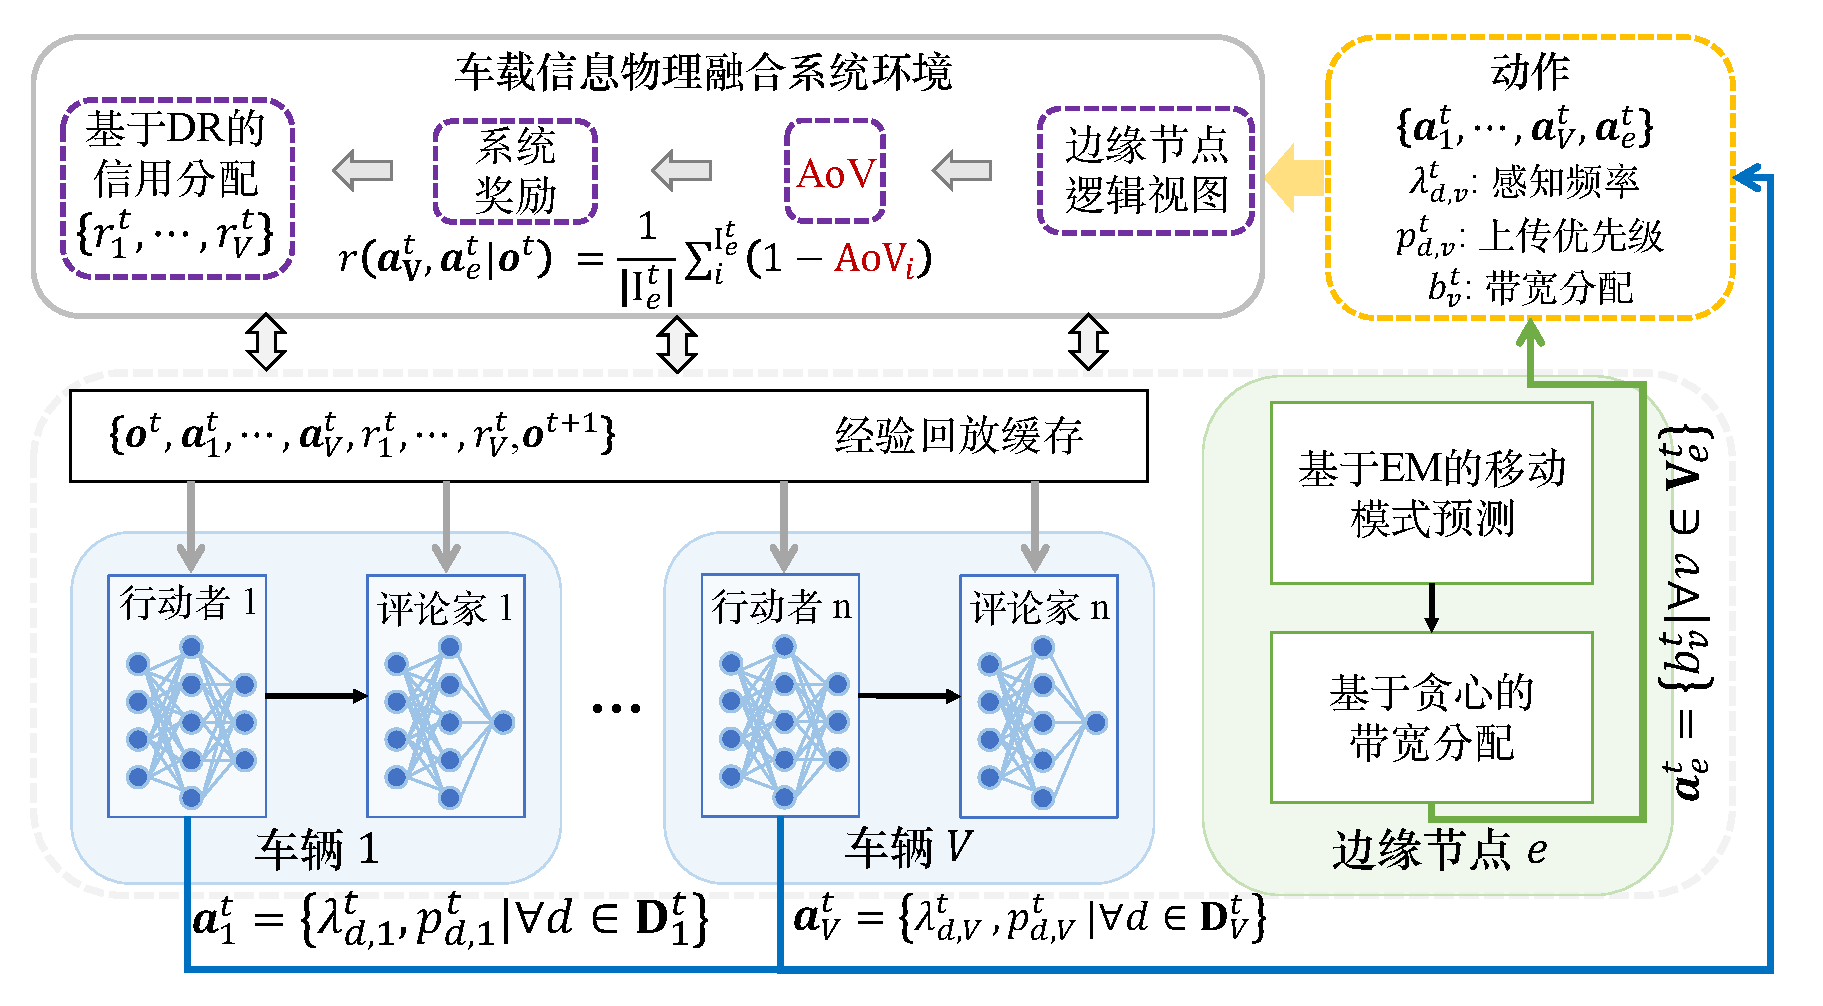
\includegraphics[width=1\columnwidth]{Fig2-4-solution-model.pdf}
  \bicaption{基于差分奖励的多智能体深度强化学习模型}{Multi-agent difference-reward-based deep reinforcement learning model}
  \label{fig 2-4}
\end{figure}

2) \textbf{动作空间}: 车辆$v$的动作空间由时间$t$的感知频率和传感信息的上传优先级组成,它被表示为:
	\begin{equation}
		\boldsymbol{a}_{v}^{t}=\{ \lambda_{d, v}^{t}, p_{d, v}^{t} \mid \forall d \in \mathbf{D}_{v}^t\}
	\end{equation}
	\noindent 其中$\lambda_{d, v}^{t}$和$p_{d, v}^{t}$分别是时间$t$内车辆$v$中信息$d$的感知频率和上传优先级。
	车辆动作的集合用$\boldsymbol{a}_{\mathbf{V}}^{t} = \left\{\boldsymbol{a}_{v}^{t}\mid \forall v \in \mathbf{V}\right\}$表示。
	边缘节点的动作是对车辆进行V2I带宽分配,其表示为:
	\begin{equation}
		\boldsymbol{a}_{e}^{t}=\{b_{v, e}^{t} \mid \forall v \in \mathbf{V}_{e}^{t}\}
	\end{equation}
	其中$b_{v, e}^t$是边缘节点$e$在时间$t$为车辆$v$分配的V2I带宽。
	
3) \textbf{系统奖励}: 在系统状态$\boldsymbol{o}^{t}$下,通过车辆动作$\boldsymbol{a}_{\mathbf{V}}^{t}$和边缘节点动作$\boldsymbol{a}_{e}^{t}$的系统奖励被定义为$t$时边缘节点$e$实现的VCPS质量,其计算公式为:
	\begin{equation}
		r\left(\boldsymbol{a}_{\mathbf{V}}^{t},\boldsymbol{a}_{e}^{t} \mid \boldsymbol{o}^{t}\right)=\frac{1}{\left|\mathbf{I}_e^t\right|} \sum_{\forall i \in \mathbf{I}_e^t}\left(1 -\operatorname{AoV}_{i} \right)
	\end{equation}
	
系统奖励展示了整个系统的综合表现,该表现来自于车辆和边缘节点的共同努力。
为了评估各车辆的贡献,需要将系统奖励分配给每个车辆作为个人奖励。
基于DR的信用分配方案是通过计算系统奖励与无该智能体动作所获奖励之间的差值来确定该智能体的个人奖励,可以更准确地评估每个智能体的行为,从而进一步提升所提出解决方案的性能。
因此,车辆$v$的差分奖励表示为:
\begin{equation}
r_{v}^{t}=r\left(\boldsymbol{a}_{\mathbf{V}}^{t},\boldsymbol{a}_{e}^{t} \mid \boldsymbol{o}^{t}\right)-r\left(\boldsymbol{a}_{\mathbf{V}-v}^{t},\boldsymbol{a}_{e}^{t} \mid \boldsymbol{o}^{t}\right)
\end{equation}
\noindent 其中 $r\left(\boldsymbol{a}_{\mathbf{V}-v}^{t},\boldsymbol{a}_{e}^{t} \mid \boldsymbol{o}^{t}\right)$是没有车辆$v$贡献的系统奖励,其可通过设置车辆$v$的空动作集得到。
车辆的差分奖励集合用$\boldsymbol{r}_{\mathbf{V}}^{t}=\{ r_{v}^{t} \mid \forall v \in \mathbf{V}\}$表示。

\subsection{工作流程}
本章节介绍基于差分奖励的多智能体强化学习算法的工作流程,其主要包括三个部分,即初始化、回放经验存储和训练,其详细步骤见算法2.1。

1) \textbf{初始化}: 首先,每辆车都作为一个智能体并由四个神经网络组成,即一个本地行动者网络、一个目标行动者网络、一个本地评论家网络和一个目标评论家网络。
车辆$v$的本地行动者和本地评价家网络的参数分别用$\theta_{v}^{\mu}$和$\theta_{v}^{Q}$来表示。
目标行动者和目标评论家网络的参数分别用$\theta_{v}^{\mu^{\prime}}$和$\theta_{v}^{Q^{\prime}}$表示。
其次,车辆的本地行动者和本地评价家网络的参数通过随机方式进行初始化。
目标行动者和目标评论家网络的参数初始化为与相应的本地网络一致。
\begin{align}
	\theta_{v}^{\mu^{\prime}} \leftarrow \theta_{v}^{\mu}, \forall v \in \mathbf{V}\\
	\theta_{v}^{Q^{\prime}} \leftarrow \theta_{v}^{Q}, \forall v \in \mathbf{V}
\end{align}
最后,初始化一个最大容量为$|\mathcal{B}|$的经验回放缓存以存储车辆与环境的交互经验。

\SetKwInOut{KwIn}{输入}
\SetKwInOut{KwOut}{输出}

\begin{algorithm}[h]\small
\renewcommand{\algorithmcfname}{算法}
		\caption{基于差分奖励的多智能体深度强化学习}
		\KwIn{学习率$\alpha$和$\beta$、折扣因子$\tau$、经验回放缓存$\mathcal{B}$、批大小$M$、轨迹预测时间$H$}
		\KwOut{信息感知频率$\lambda_{d, v}^{t}$、上传优先级$p_{d, v}^{t}$、带宽分配$b_{v, e}^{t}$}
		初始化网络参数\\
		初始化经验回放缓存$\mathcal{B}$\\
        \For{\songti{迭代次数} $= 1$ \songti{到最大迭代次数}}{
            初始化一个随机过程 $\mathcal{N}$ 以进行探索 \\
            接收初始系统状态 $\boldsymbol{o}_{1}$\\
            \For{\songti{时间片} $t = 1$ \songti{到} $T$}{
            	\For{\songti{车辆} $v=1$ \songti{到} $V$ }{
            			接收本地观测值 $\boldsymbol{o}_{v}^{t}$ \\
                    	选择一个动作 $\boldsymbol{a}_{v}^{t}=\boldsymbol{\mu}_{v}\left(\boldsymbol{o}_{v}^{t} \mid \theta_{v}^{\mu}\right)+\mathcal{N}_{t}$ \\
            		得到所需信息 $\mathbf{D}_{v,\operatorname{R}}^{t}$\\
        		通过基于EM方法利用历史相对距离来预测移动模式\\
        		预测未来的轨迹 $\operatorname{Traj}_{v}^{t}$ \\
        		计算平均距离$\operatorname{\bar{dis}}_{v, e}^{t}$
            	}
        	\For{\songti{车辆} $v=1$ \songti{到} $V$ }{
        		通过VBA策略分配带宽 $b_{v, e}^{t}$ 给车辆 $s$\\}
            	接收系统奖励 $r\left(\boldsymbol{a}_{\mathbf{V}}^{t},\boldsymbol{a}_{e}^{t} \mid \boldsymbol{o}^{t}\right)$ 和下一时刻系统状态 $\boldsymbol{o}^{t+1}$\\
            	划分系统奖励为差分奖励$\boldsymbol{r}_{\mathbf{V}}^{t}$\\
            	存储 $\left(\boldsymbol{o}^{t}, \boldsymbol{a}_{\mathbf{V}}^{t}, \boldsymbol{r}_{\mathbf{V}}^{t}, \boldsymbol{o}^{t+1}\right)$ 到经验回放缓存 $\mathcal{B}$
            }
            \For{\songti{车辆} $v=1$ \songti{到} $V$ }{
            		从经验回放缓存$\mathcal{B}$随机采样 $M$ 最小批\\
            		更新本地行动者和评论家网络参数\\
            	}
            	更新目标行动者和评论家网络参数
       	}
\label{algorithm 2-1}
\end{algorithm}

2) \textbf{回放经验存储}:
在每次迭代的开始,初始化一个随机过程$\mathcal{N}$用于增加智能体探索。
车辆$v$在时间$t$的行动是由本地行动者网络根据其对系统状态的本地观察得到的。
\begin{equation}
	\boldsymbol{a}_{v}^{t}=\boldsymbol{\mu}_{\boldsymbol{v}}\left(\boldsymbol{o}_{v}^{t} \mid \theta_{v}^{\mu}\right)+\mathcal{N}_{t}
\end{equation}
\noindent 其中,$\mathcal{N}_{t}$是一个由随机过程$\mathcal{N}$得到的探索噪音,以增加车辆动作的多样性。

边缘节点$e$根据车辆预测轨迹和视图需求,通过VBA方案分配V2I带宽。
首先,边缘节点$e$根据车辆和边缘节点之间的历史距离,使用期望最大化(Expectation-Maximization, EM)方法\cite{hofmann2001unsupervised} 预测车辆的移动模式。
然后,根据基于EM的移动性预测模式,预测车辆$v$在未来$H$时间片的轨迹,用$\operatorname{Traj}_{v}^{t} = \{ \hat{l}_{v}^{t+1}, \dots, \hat{l}_{v}^{t+h}, \dots, \hat{l}_{v}^{t+H}\}$表示,其中$\hat{l}_{v}^{t+h}$是车辆$v$在时间$t+h$的预测位置。
因此,车辆在边缘节点之间的平均距离的计算公式如下:
\begin{equation}
	\operatorname{\bar{dis}}_{v, e}^{t} = \frac{1}{H} {\sum_{\forall h \in [1, H]} \widehat{\operatorname{dis}}_{v, e}^{t+h}}
\end{equation}
其中,$\widehat{\operatorname{dis}}_{v, e}^{t+h}$ 是车辆$v$预测位置与边缘节点的距离,即$\widehat{\operatorname{dis}}_{v, e}^{t+h}=\operatorname{distance}(\hat{l}_{v}^{t+h}, l_{e})$。

那么,由车辆$v$感知到的并被视图$i$在时间$t$所需的信息集表示为:
\begin{equation}
	\mathbf{D}_{v, i}^{t} = \left\{ d \mid  d \in \mathbf{D}_{v}^t \cap  \mathbf{D}_i \right\}
\end{equation}
因此,由车辆$v$感知并被边缘节点$e$上视图在时间$t$需要的信息集合表示为:
\begin{equation}
	\mathbf{D}_{v, {\mathbf{I}_e^t}}^{t} = \{ d \mid  d \in \bigcup_{\forall v \in V_e^t} \mathbf{D}_{v, i}^{t}\}
\end{equation}
\noindent 该集合的大小记为$|\mathbf{D}_{v, {\mathbf{I}_e^t}}^{t}|$, 并可通过下式得到:
\begin{equation}
	|\mathbf{D}_{v, {\mathbf{I}_e^t}}^{t}| = \sum_{\forall d \in \mathbf{D}_{v, {\mathbf{I}_e^t}}^{t}}|d|
\end{equation}
最后,边缘节点$e$为车辆$v$分配的V2I带宽由下式计算:
\begin{equation}
	b_{v, e}^{t} =\frac{b_{e}} {\omega+\operatorname{rank}_{v}}
\end{equation}
\noindent 其中$\omega$为常数,$\operatorname{rank}_{v}$为车辆$v$按$| \mathbf{D}_{v, {\mathbf{I}_e^t}}^{t}|$的序列降序并按$\operatorname{\bar{dis}}_{v, e}^{t}$的序列升序排列的序列名次。

在确定车辆和边缘节点的联合动作后,以实现的VCPS质量作为系统奖励$r\left(\boldsymbol{a}_{\mathbf{V}}^{t},\boldsymbol{a}_{e}^{t} \mid \boldsymbol{o}^{t}\right)$,并通过基于DR的信用分配方案进一步划分为差分奖励$\boldsymbol{r}_{\mathbf{V}}^{t}$。
最后,包括当前系统状态$\boldsymbol{o}^{t}$、车辆动作$\boldsymbol{a}_{\mathbf{V}}^{t}$、差分奖励$\boldsymbol{r}_{\mathbf{V}}^{t}$和下一时刻系统状态$\boldsymbol{o}^{t+1}$在内的交互经验被存储在经验回放缓存$\mathcal{B}$。

3) \textbf{训练}: 从经验回放缓存$\mathcal{B}$中随机抽取$M$样本的小批量,用于训练车辆中的行动者和评论家网络,其中单个样本用$(\boldsymbol{o}_{v}^{m}, \boldsymbol{a}_{\mathbf{V}}^{m}, \boldsymbol{r}_{\mathbf{V}}^{m}, \boldsymbol{o}_{v}^{m+1})$表示。
本地行动者网络和本地评论家网络的参数以学习率$\alpha$和$\beta$更新
车辆$v$的本地评论家网络的损失函数通过下式计算:
\begin{equation}
	\mathcal{L}\left(\theta_{v}^{Q}\right)=\frac{1}{M} \Sigma_{m}\left(\eta_{m}-Q_{v}\left(\boldsymbol{o}_{v}^{m}, \boldsymbol{a}_{\mathbf{V}}^{m} \mid \theta_{v}^{Q}\right)\right)^{2}
\end{equation}
\noindent 其中,$\eta_{m}$是由目标评论家网络产生的目标值,$\eta_{m}=r_{v}^{m}+\tau Q_{v}^{\prime}(\boldsymbol{o}_{v}^{m+1}, \boldsymbol{a}_{\mathbf{V}}^{m+1} \mid \theta_{v}^{Q^{\prime}})$,$\tau$是奖励折扣因子。
车辆$v$在时间$m+1$的行动是由目标行动者网络根据对下一时刻系统状态的局部观察得到的,即$\boldsymbol{a}_{\mathbf{V}}^{m+1}=\mu_{v}^{\prime}(\boldsymbol{o}_{v}^{m+1} \mid \theta_{v}^{\mu^{\prime}})$。
车辆$v$的本地行动者网络的参数通过策略网络梯度更新。
\begin{equation}
	\nabla_{\theta_{v}^{\mu}} \mathcal{J} \approx \frac{1}{M} \sum_{m} \nabla_{\boldsymbol{a}_{\mathbf{V}}^{m}} Q_{v}\left(\boldsymbol{o}_{v}^{m}, \boldsymbol{a}_{\mathbf{V}}^{m} \mid \theta_{v}^{Q}\right) \nabla_{\theta_{v}^{\mu}} \mu_{v}\left(\boldsymbol{o}_{v}^{m+1} \mid \theta_{v}^{\mu}\right)
\end{equation}
最后,车辆更新目标网络的参数。
\begin{align}
	\theta_{v}^{\mu^{\prime}} &\leftarrow n_{v} \theta_{v}^{\mu}+(1-n_{v})  \theta_{v}^{\mu^{\prime}}, \forall v \in \mathbf{V}\\
	\theta_{v}^{Q^{\prime}} &\leftarrow n_{v} \theta_{i}^{Q}+(1-n_{v})  \theta_{v}^{Q^{\prime}}, \forall v \in \mathbf{V}
\end{align}
\noindent 其中 $n_{v} \ll 1, \forall v \in \mathbf{V} $。

\section{实验结果与分析}\label{section 2-6}

\subsection{基本设置}
本章使用Python 3.9和PyTorch 1.11.0实现了一个仿真模型,以评估MADR的性能。
该仿真模型基于一台配备AMD Ryzen 9 5950X 16核处理器@3.4 GHz、两个NVIDIA GeForce RTX 3090图形处理单元和64 GB内存的Ubuntu 20.04服务器。
特别地,本章使用真实世界的车辆轨迹构建了三种交通场景,这些轨迹来自滴滴GAIA数据集,包括:1)中国成都市青羊区3平方公里区域,2016年11月16日8:00至8:05;2)同一区域,同日23:00至23:05;3)中国西安碑林区3平方公里区域,2016年11月27日8:00至8:05。
车辆轨迹的具体分析包括车辆轨迹总数、车辆平均停留时间(Average Dwell Time,ADT)、停留时间方差(Variance of Dwell Time, VDT)、平均车辆数(Average Vehicle Number, AVN)、车辆数方差(Variance of Vehicle Number, VVN)、车辆平均速度(Average Vehicle Speed,AVS)和车辆速度方差(Variance of Vehicle Speed,VVS)的详细统计,其总结在表\ref{table 2-1}中。
图\ref{fig 2-5}显示了调度周期内车辆分布的热力图,以更好地展示不同场景下的交通特征。
比较图\ref{fig 2-5}(a)、图\ref{fig 2-5}(b)和图\ref{fig 2-5}(c),可以发现工作日高峰期(即2016年11月16日星期三8:00左右)的车辆密度远远高于同一地区的夜间(即同日23点左右),也比周末的高峰期(即2016年11月27日星期日8:00左右)高得多。
此外,可以观察到在图\ref{fig 2-5}(c)中车辆分布完全不同,因为车辆轨迹是从另一个城市提取的。

实验参数设置描述如下:
信息的数据大小均匀分布在[100 B, 1 MB]的范围内。
每辆车的传输功率为1 mW。
V2I通信的 AWGN 和路径损耗指数分别设置为-90 dBm和3 \cite{sadek2009distributed}。
V2I通信的信道衰减增益遵循均值为2、方差为0.4的高斯分布。
边缘节点的带宽被设置为3 MHz \cite{wang2019delay}。
噪声的不确定性遵循[0,3] dB的均匀分布 \cite{tandra2008snr}。

\begin{table}[h]\small
\centering
\bicaption{不同场景的交通特征}{Traffic characteristics of each scenario}
\resizebox{\columnwidth}{!}{%
\begin{tabular}[t]{cccccccc}
\toprule
场景&轨迹&ADT (s)&VDT&AVN&VVN&AVS (m/s)&VVS\\
\midrule
1&718&198.3&123.8&474.6&11.6&5.22&2.61\\
2&359&173.7&124.1&207.9&3.93&7.30&3.16\\
3&206&145.5&114.7&99.9&7.65&8.06&3.70\\
\bottomrule
\end{tabular}}
\label{table 2-1}
\end{table}

\begin{figure}[h]
\centering
  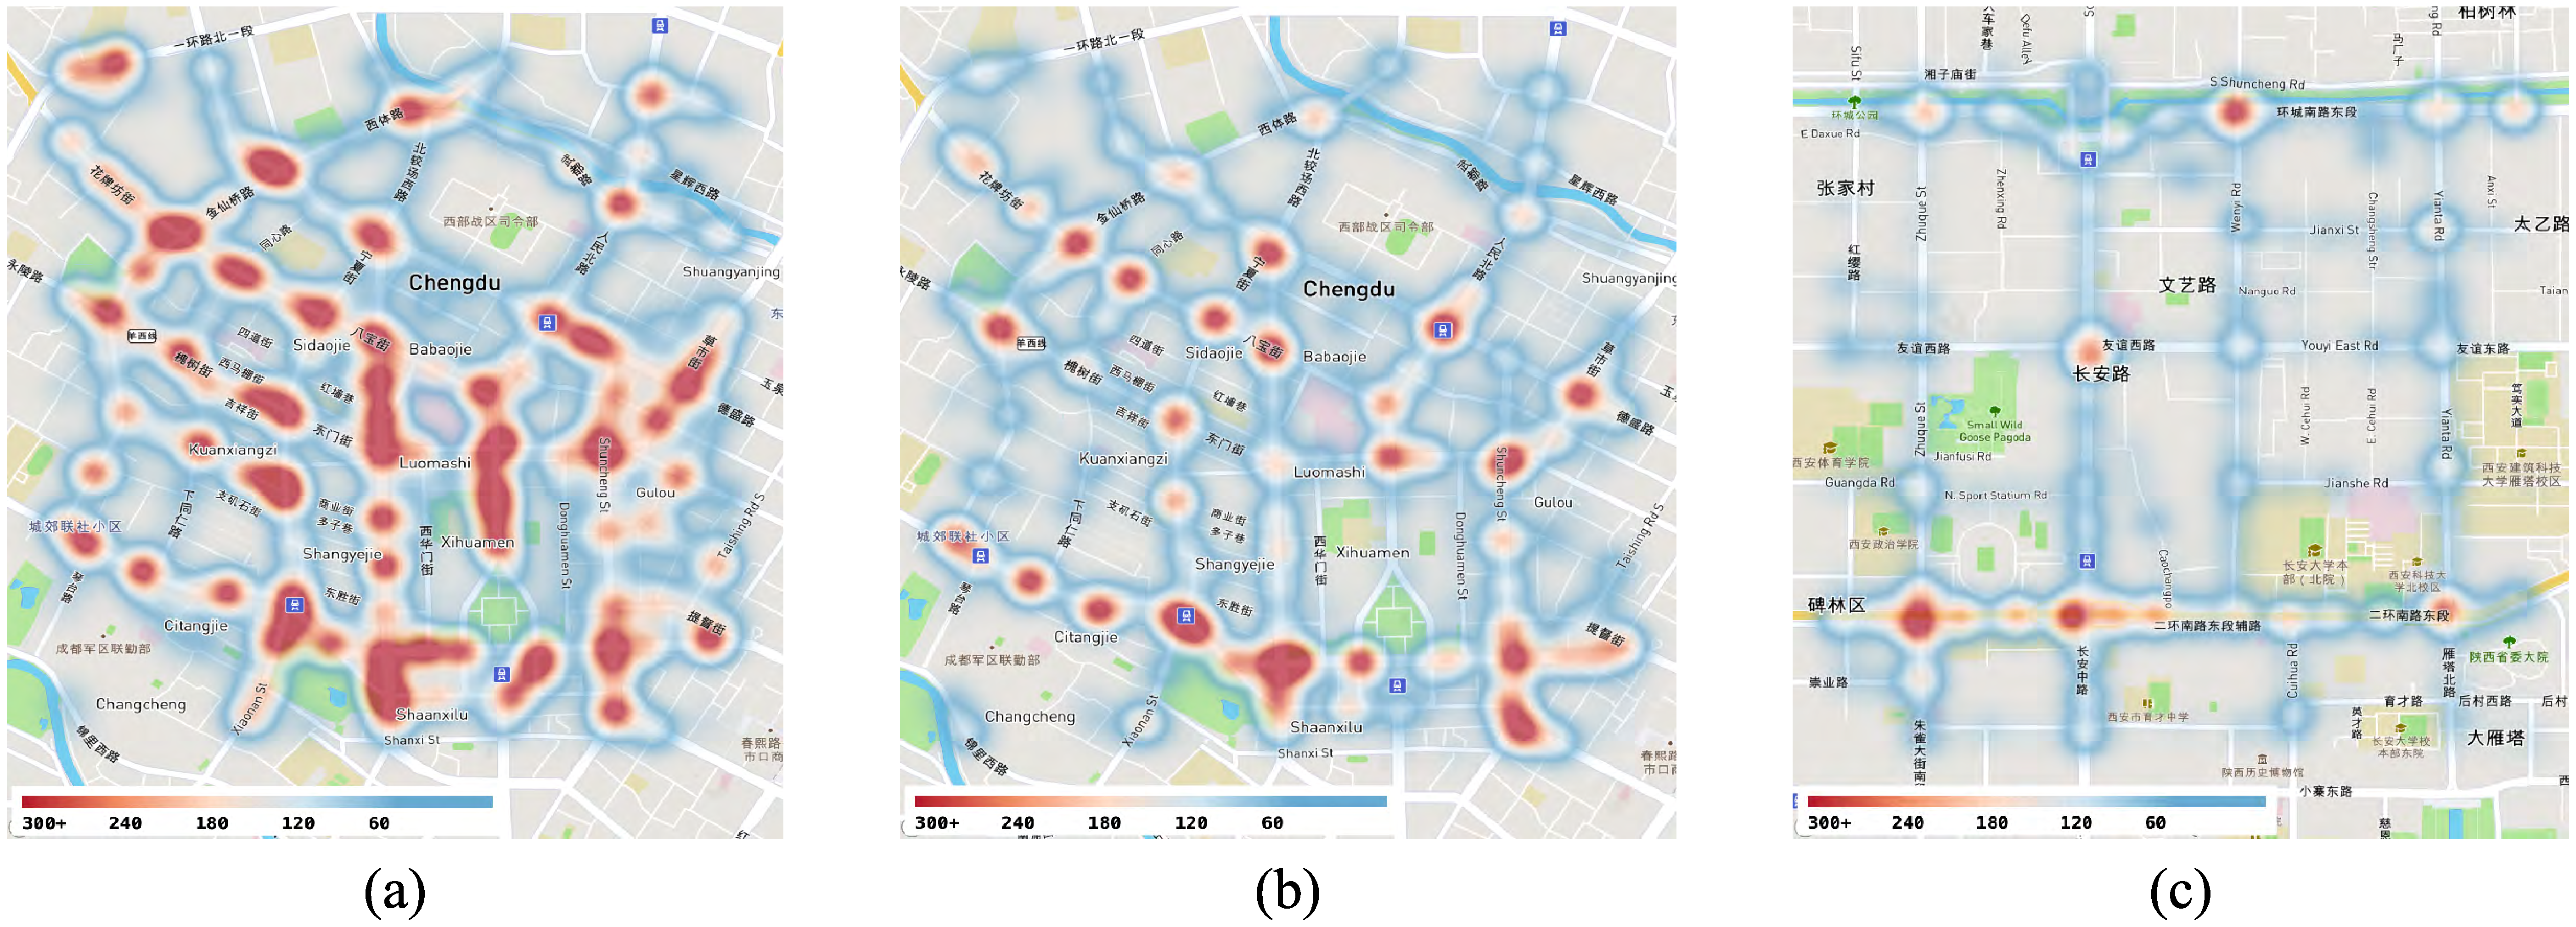
\includegraphics[width=1\columnwidth]{Fig2-5-heat-map.pdf}
  \bicaption[不同场景下的车辆分布热力图]{不同场景下的车辆分布热力图。(a) 场景1(b)场景2(c)场景3}[Heat map of the distribution of vehicles under different scenarios]{Heat map of the distribution of vehicles under different scenarios. (a) Scenario 1 (b) Scenario 2 (c) Scenario 3}
  \label{fig 2-5}
\end{figure} 

MADR的架构和超参数描述如下:
本地行动者网络是一个四层全连接的神经网络,其中包含两个隐藏层,其神经元数量分别为64和32。
目标行动者网络结构与本地行动者网络相同。
本地评论家网络是一个四层全连接的神经网络,其中包含两个隐藏层,其神经元数量分别为128和64。
目标评论家网络的结构与本地评论家网络相同。
使用整流线性单元(Rectified Linear Unit, ReLU)作为激活函数,使用自适应矩估计(Adaptive Moment Estimation, Adam)优化器更新网络权重,本地行动者网络和本地评论家网络学习率均为 0.001,奖励折扣因子为 0.996。
经验回放缓存$|\mathcal{B}|$的大小为100000,批大小为512。
此外,本章还实现了以下四种可比较的算法。

\begin{itemize}
	\item \textbf{随机分配}: 在每个时间片中,随机选择一个关于确定感知频率、上传优先级和V2I带宽分配的动作。
	\item \textbf{集中式深度确定性策略梯度}\cite{mlika2022deep}: 在边缘节点实现一个智能体,根据系统状态以集中的方式确定感知频率、上传优先级和V2I带宽分配。同时,智能体接收系统奖励以评估其贡献。
	\item \textbf{多智能体行动者-评论家}\cite{he2021efficient}: 实现了车辆中的智能体,基于本地车联网环境观测来决定感知频率和上传优先级,以及边缘节点中的智能体来决定V2I带宽分配。每个智能体都接收相同的系统奖励以评估其贡献。
	\item \textbf{采用VBA策略的多智能体行动者-评论家}: 为了更好地分配V2I带宽,本章进一步设计了一个多智能体行动者-评论家算法的变体,其中边缘节点基于VBA策略来分配V2I带宽,其余部分与MAAC算法一致。
\end{itemize}

此外,本章还设计了以下指标用于性能评估。
\begin{itemize}
	\item \textbf{累积奖励} (Cumulative Reward, CR): 定义为调度期间的累积系统奖励, 其计算方法为:
		\begin{equation}
			\operatorname{CR} = \sum_{\forall t \in \mathbf{T}} r\left(\boldsymbol{a}_{v}^{t},\boldsymbol{a}_{e}^{t} \mid \boldsymbol{o}^{t}\right)
		\end{equation}
	\item \textbf{平均奖励的构成} (Composition of Average Reward, CAR): 定义为归一化的时效性、完整性和一致性在平均奖励中的百分比,其表示为:
		\begin{equation}
			\operatorname{CAR} \triangleq <\frac{3}{10}(1-\hat{\Xi}_{i}),\frac{4}{10}(1-\hat{\Phi}_{i}), \frac{3}{10}(1-\hat{\Psi}_{i})>
		\end{equation}
	\item \textbf{平均排队时间} (Average Queuing Time, AQT): 定义为感知信息的排队时间之和除以调度期$T$内的信息数量,其计算方法为:
		\begin{equation}
			\operatorname{AQT} =\sum_{\forall t \in \mathbf{T}} \left \{ \frac{\sum_{v \in \mathbf{V}} \sum_{\forall d \subseteq \mathbf{D}_{v}^t} \frac{\operatorname{q}_{d, v}^t}{|\mathbf{D}_{v}^t|} }{V} \right\} \bigg/ T
		\end{equation}
	\item \textbf{服务率} (Service Ratio, SR): 定义为满足完整性要求的视图的数量在调度期间$\mathbf{T}$所需的视图总数的占比,其计算方法是:
		\begin{equation}
			\operatorname{SR} = \frac{\sum_{\forall t \in \mathbf{T}}\sum_{\forall i \in \mathbf{I}_e^t} \mathds{1}\{\Phi_{i} \geq \Phi_{th}\}}{ \sum_{\forall t \in \mathbf{T}} |\mathbf{I}_e^t|}
		\end{equation}
	其中 $\Phi_{th}$ 是完整性阈值。
\end{itemize}

\subsection{实验结果与分析}

\textbf{1) 算法收敛性:}
图\ref{fig 2-6}比较了五种算法在收敛速度和CR值方面的表现。结果显示,本章提出的MADR算法收敛速度最快(约660次迭代),并获得了最高的CR值(约357)。相比之下,C-DDPG、MAAC和MAAC-VBA分别需要大约4500次、950次和870次迭代才能收敛,并分别达到约307、290和315的CR值。RA作为基线算法的CR值约为241。值得注意的是,与C-DDPG、MAAC和MAAC-VBA相比,MADR算法在CR值方面分别实现了大约16.3\%、23.1\%和13.3\%的增加,同时在收敛速度方面分别提升了大约6.8倍、1.4倍和1.3倍。这主要是因为MADR算法旨在维护车辆的稳定通信环境,从而使车辆中的行动者和评论家网络的训练更加有效。另外,由于MADR的动作空间较小,相比于C-DDPG,MADR更容易收敛,因为C-DDPG需要同时决定感知频率、上传优先级和V2I带宽分配。

\begin{figure}[h]
\centering
  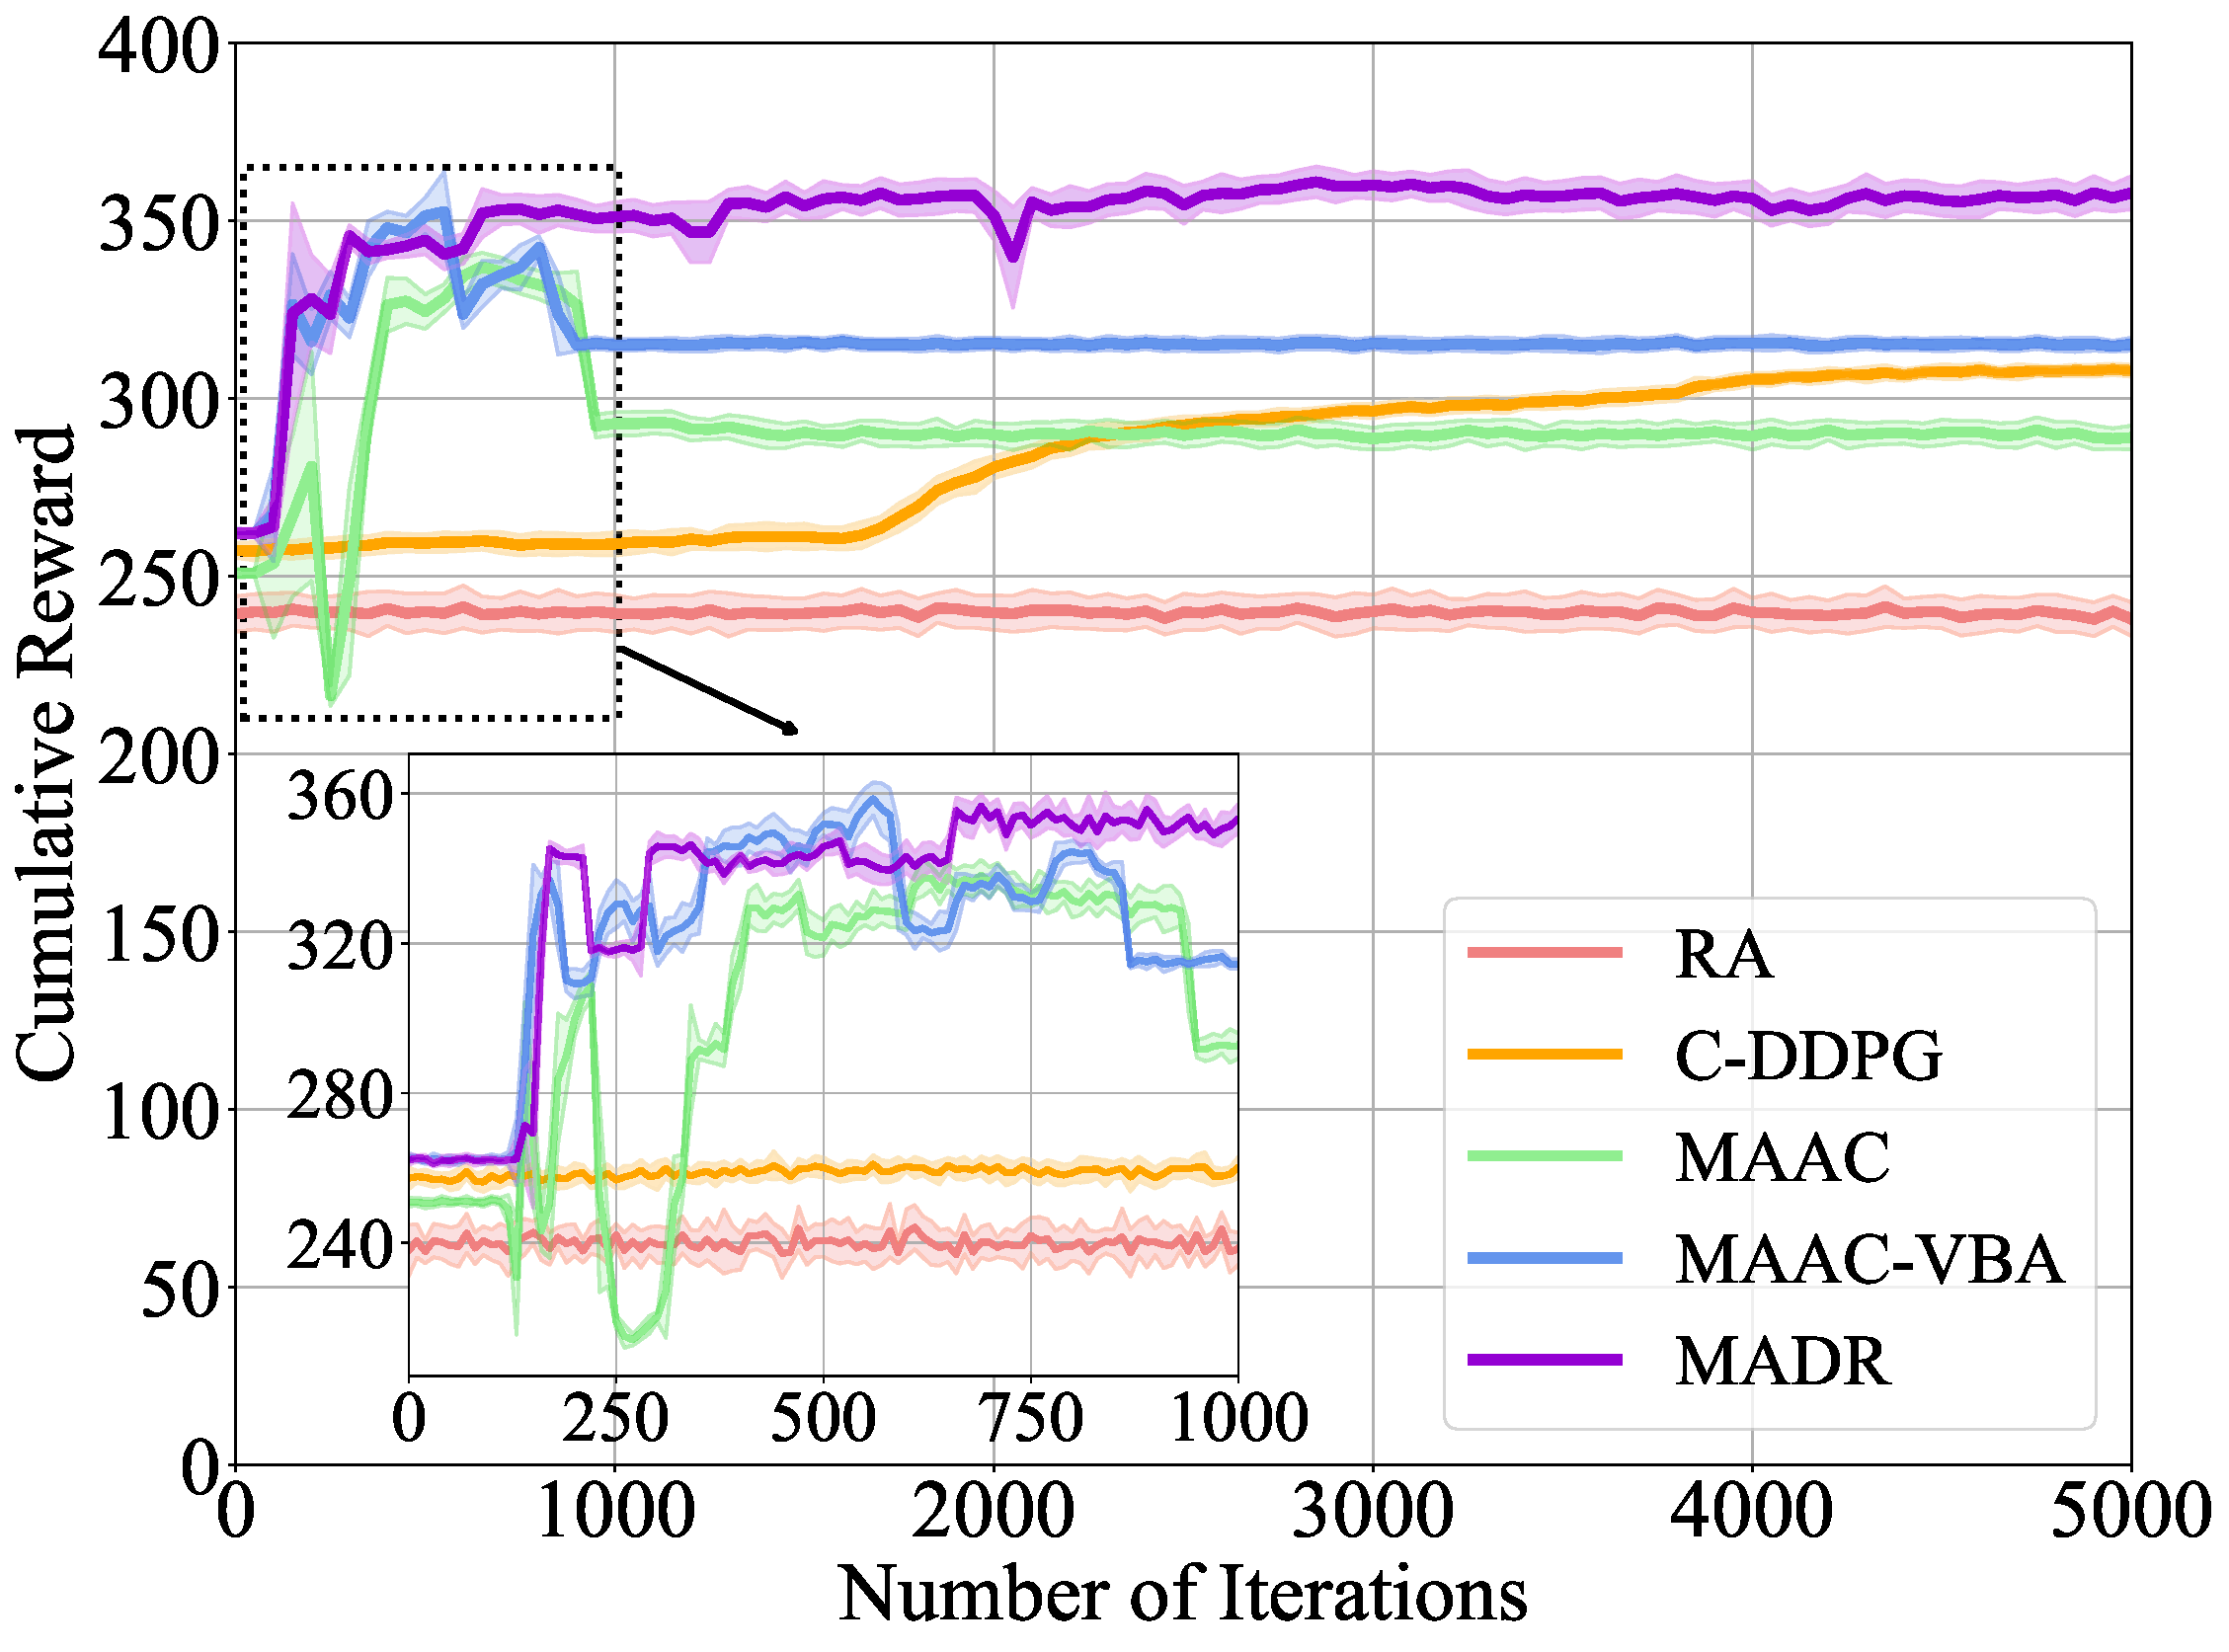
\includegraphics[width=0.75\columnwidth]{Fig2-6-convergence.pdf}
  \bicaption{算法收敛性比较}{Convergence comparison}
  \label{fig 2-6}
\end{figure} 

\begin{figure}[h]
  \centering
  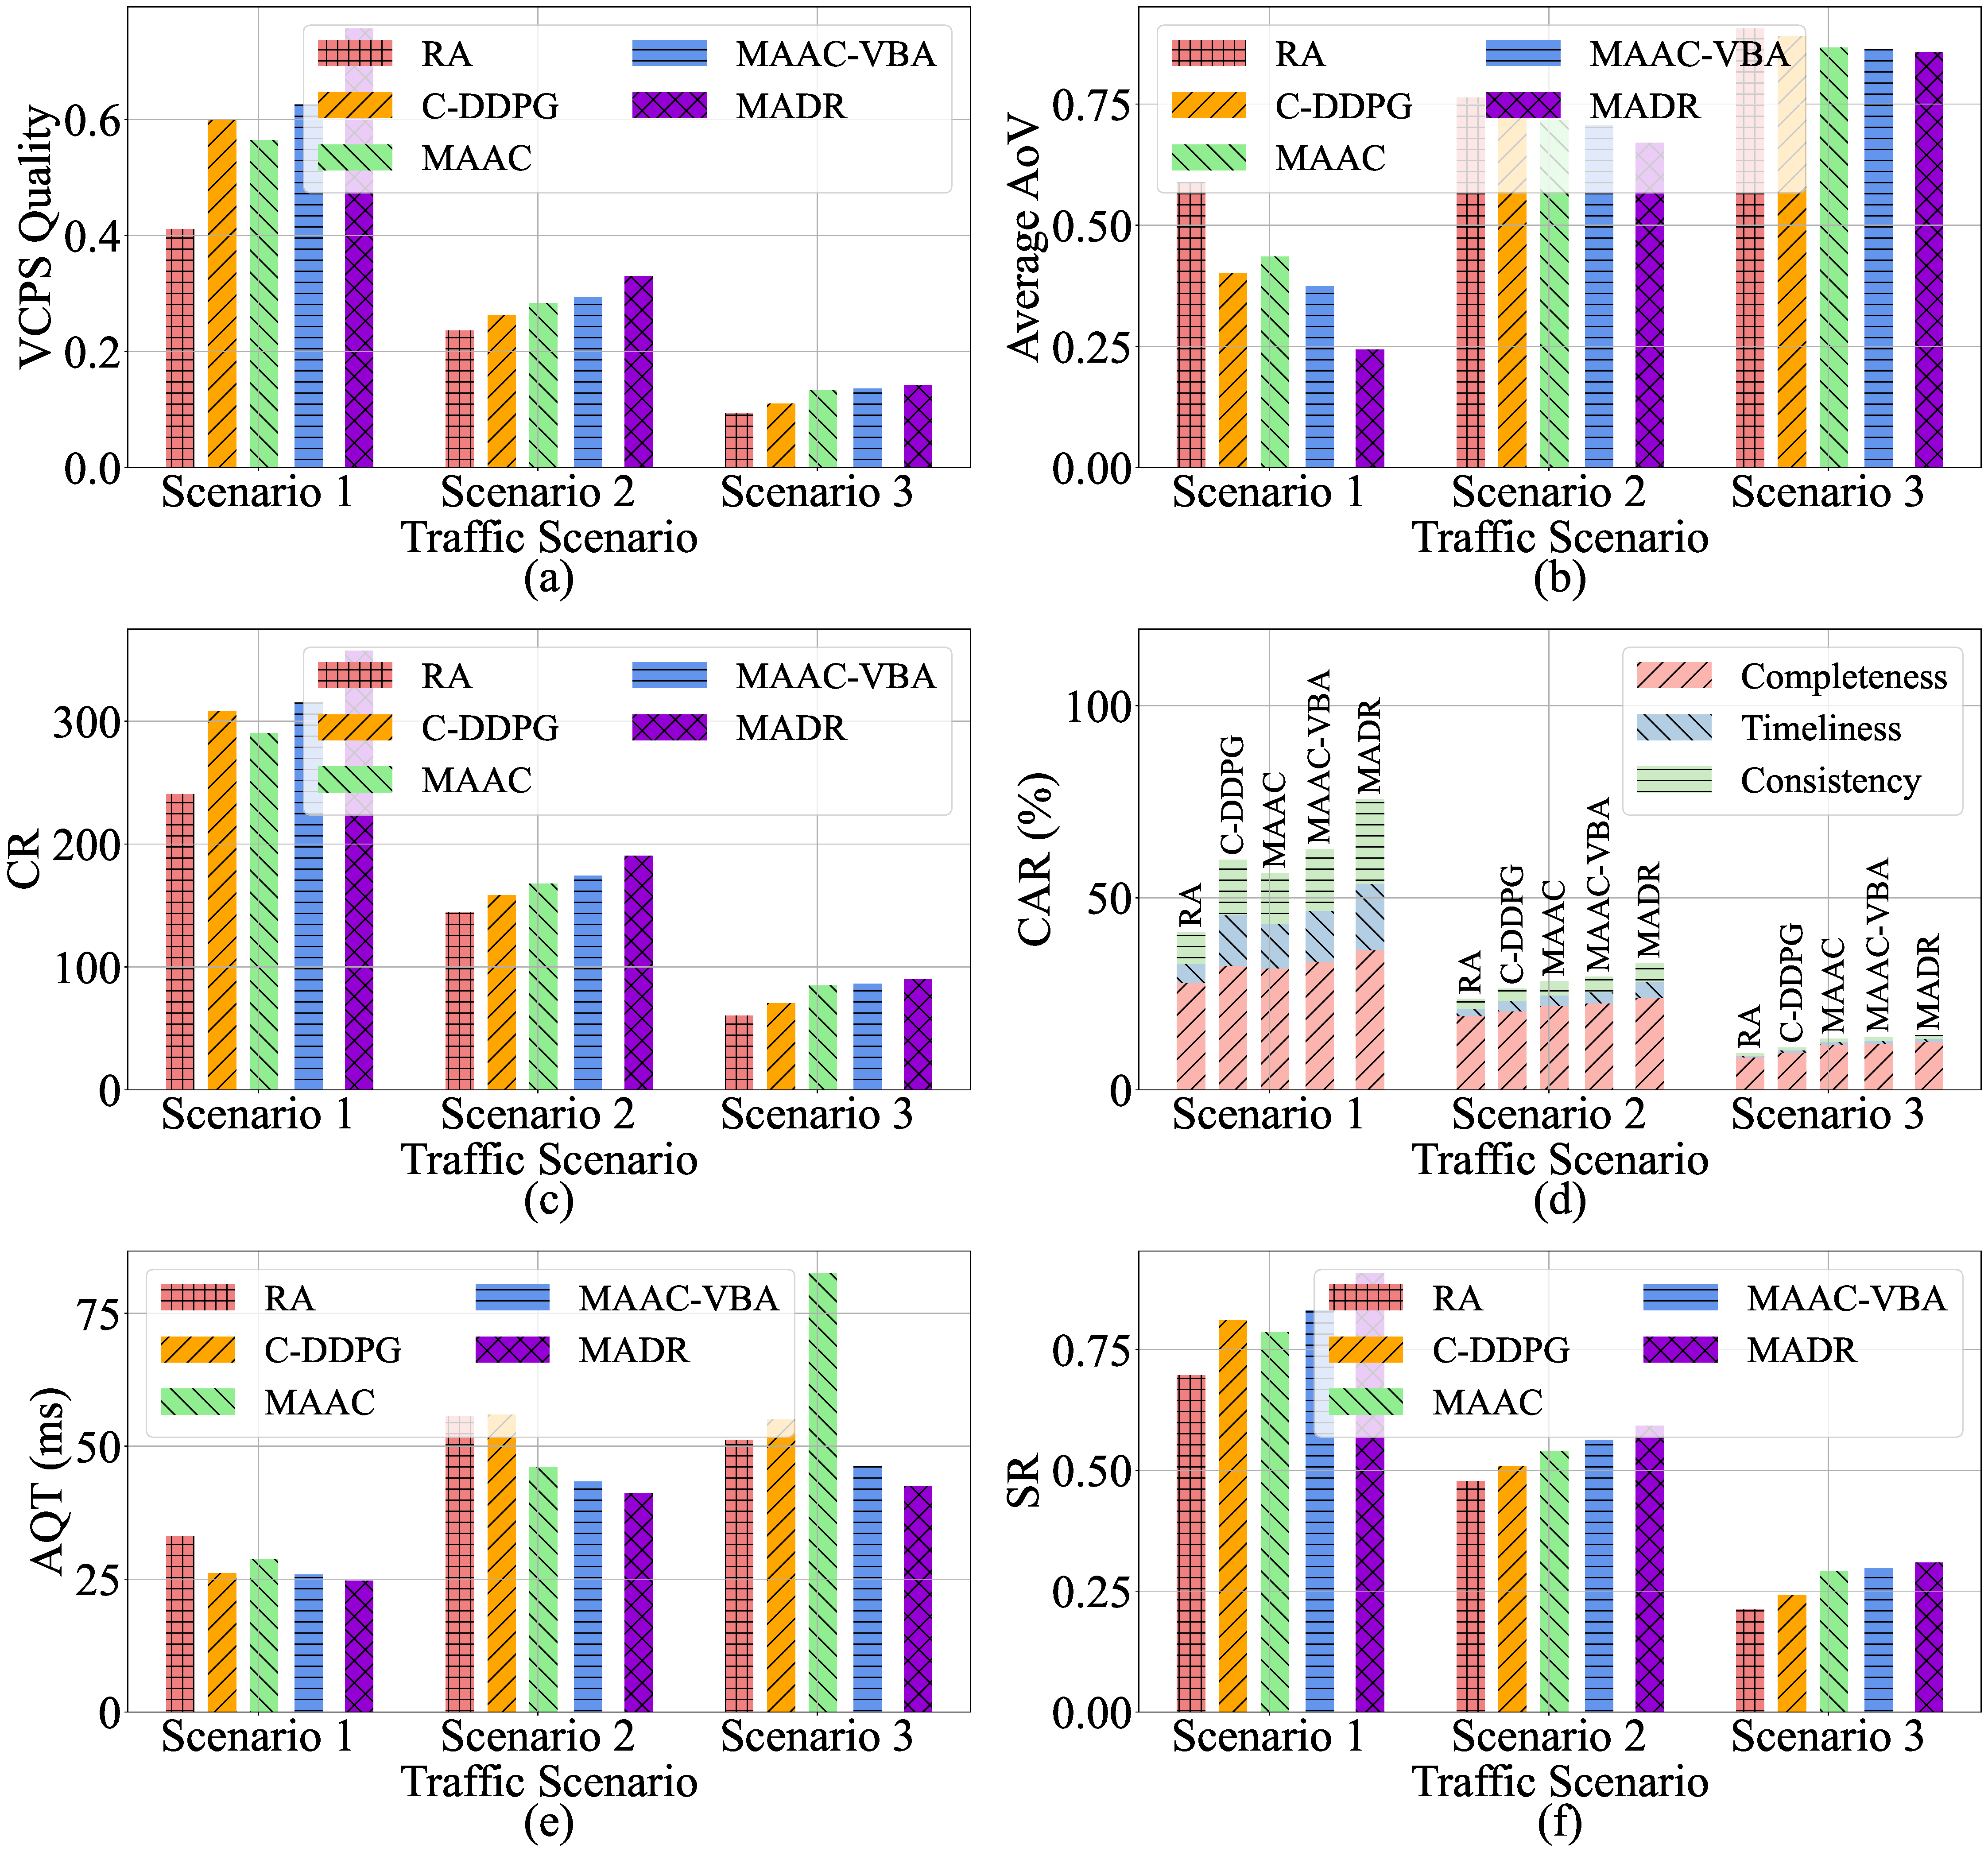
\includegraphics[width=1\columnwidth]{Fig2-7-different-scenarios.pdf}
  \bicaption[不同交通场景下的性能比较]{不同交通场景下的性能比较。(a)车载信息物理融合系统质量(b)平均 AoV(c)累积奖励(d)平均奖励的构成(e)平均排队时间(f)服务率}[Performance comparison under different traffic scenarios]{Performance comparison under different traffic scenarios. (a) Vehicular cyber-physical system quality (b) Average age of view (c) Cumulative reward (d) Composition of average reward (e) Average queuing time (f) Service ratio}
  \label{fig 2-7}
\end{figure}

\textbf{2) 交通场景的影响:}
图\ref{fig 2-7}比较了五种算法在不同交通场景下的表现。图\ref{fig 2-7}(a) 显示了五种算法在VCPS质量方面的比较。如图所示,MADR算法在所有场景下都实现了最高的VCPS质量,比RA、C-DDPG、MAAC和MAAC-VBA分别平均提高了58.0\%、27.1\%、19.1\%和12.5\%的VCPS质量。图\ref{fig 2-7}(b) 显示了五种算法在平均AoV方面的比较。所有场景下,MADR都实现了最低的平均AoV。图\ref{fig 2-7}(c) 显示了五种算法在CR方面的比较。结果表明,MADR实现的CR高于RA、C-DDPG、MAAC和MAAC-VBA。在场景3下,MADR和MAAC-VBA的CR相似,原因是场景3中较低的车辆密度和较高的车辆动态性使得数据上传比场景1和2中更加困难。图\ref{fig 2-7}(d) 将平均奖励分解成时效性、完整性和一致性三个部分的比例,以显示五种算法在这些方面的表现。在场景3下,时效性和一致性都非常小,这主要是因为当视图不完整时,时效性和一致性的要求很难得到满足。图\ref{fig 2-7}(e) 和图\ref{fig 2-7}(f) 显示了五种算法在不同场景下的AQT和SR比较。结果表明,MADR实现了最低的AQT,并在所有场景下保持最高的SR。

\begin{figure}[h]
  \centering
  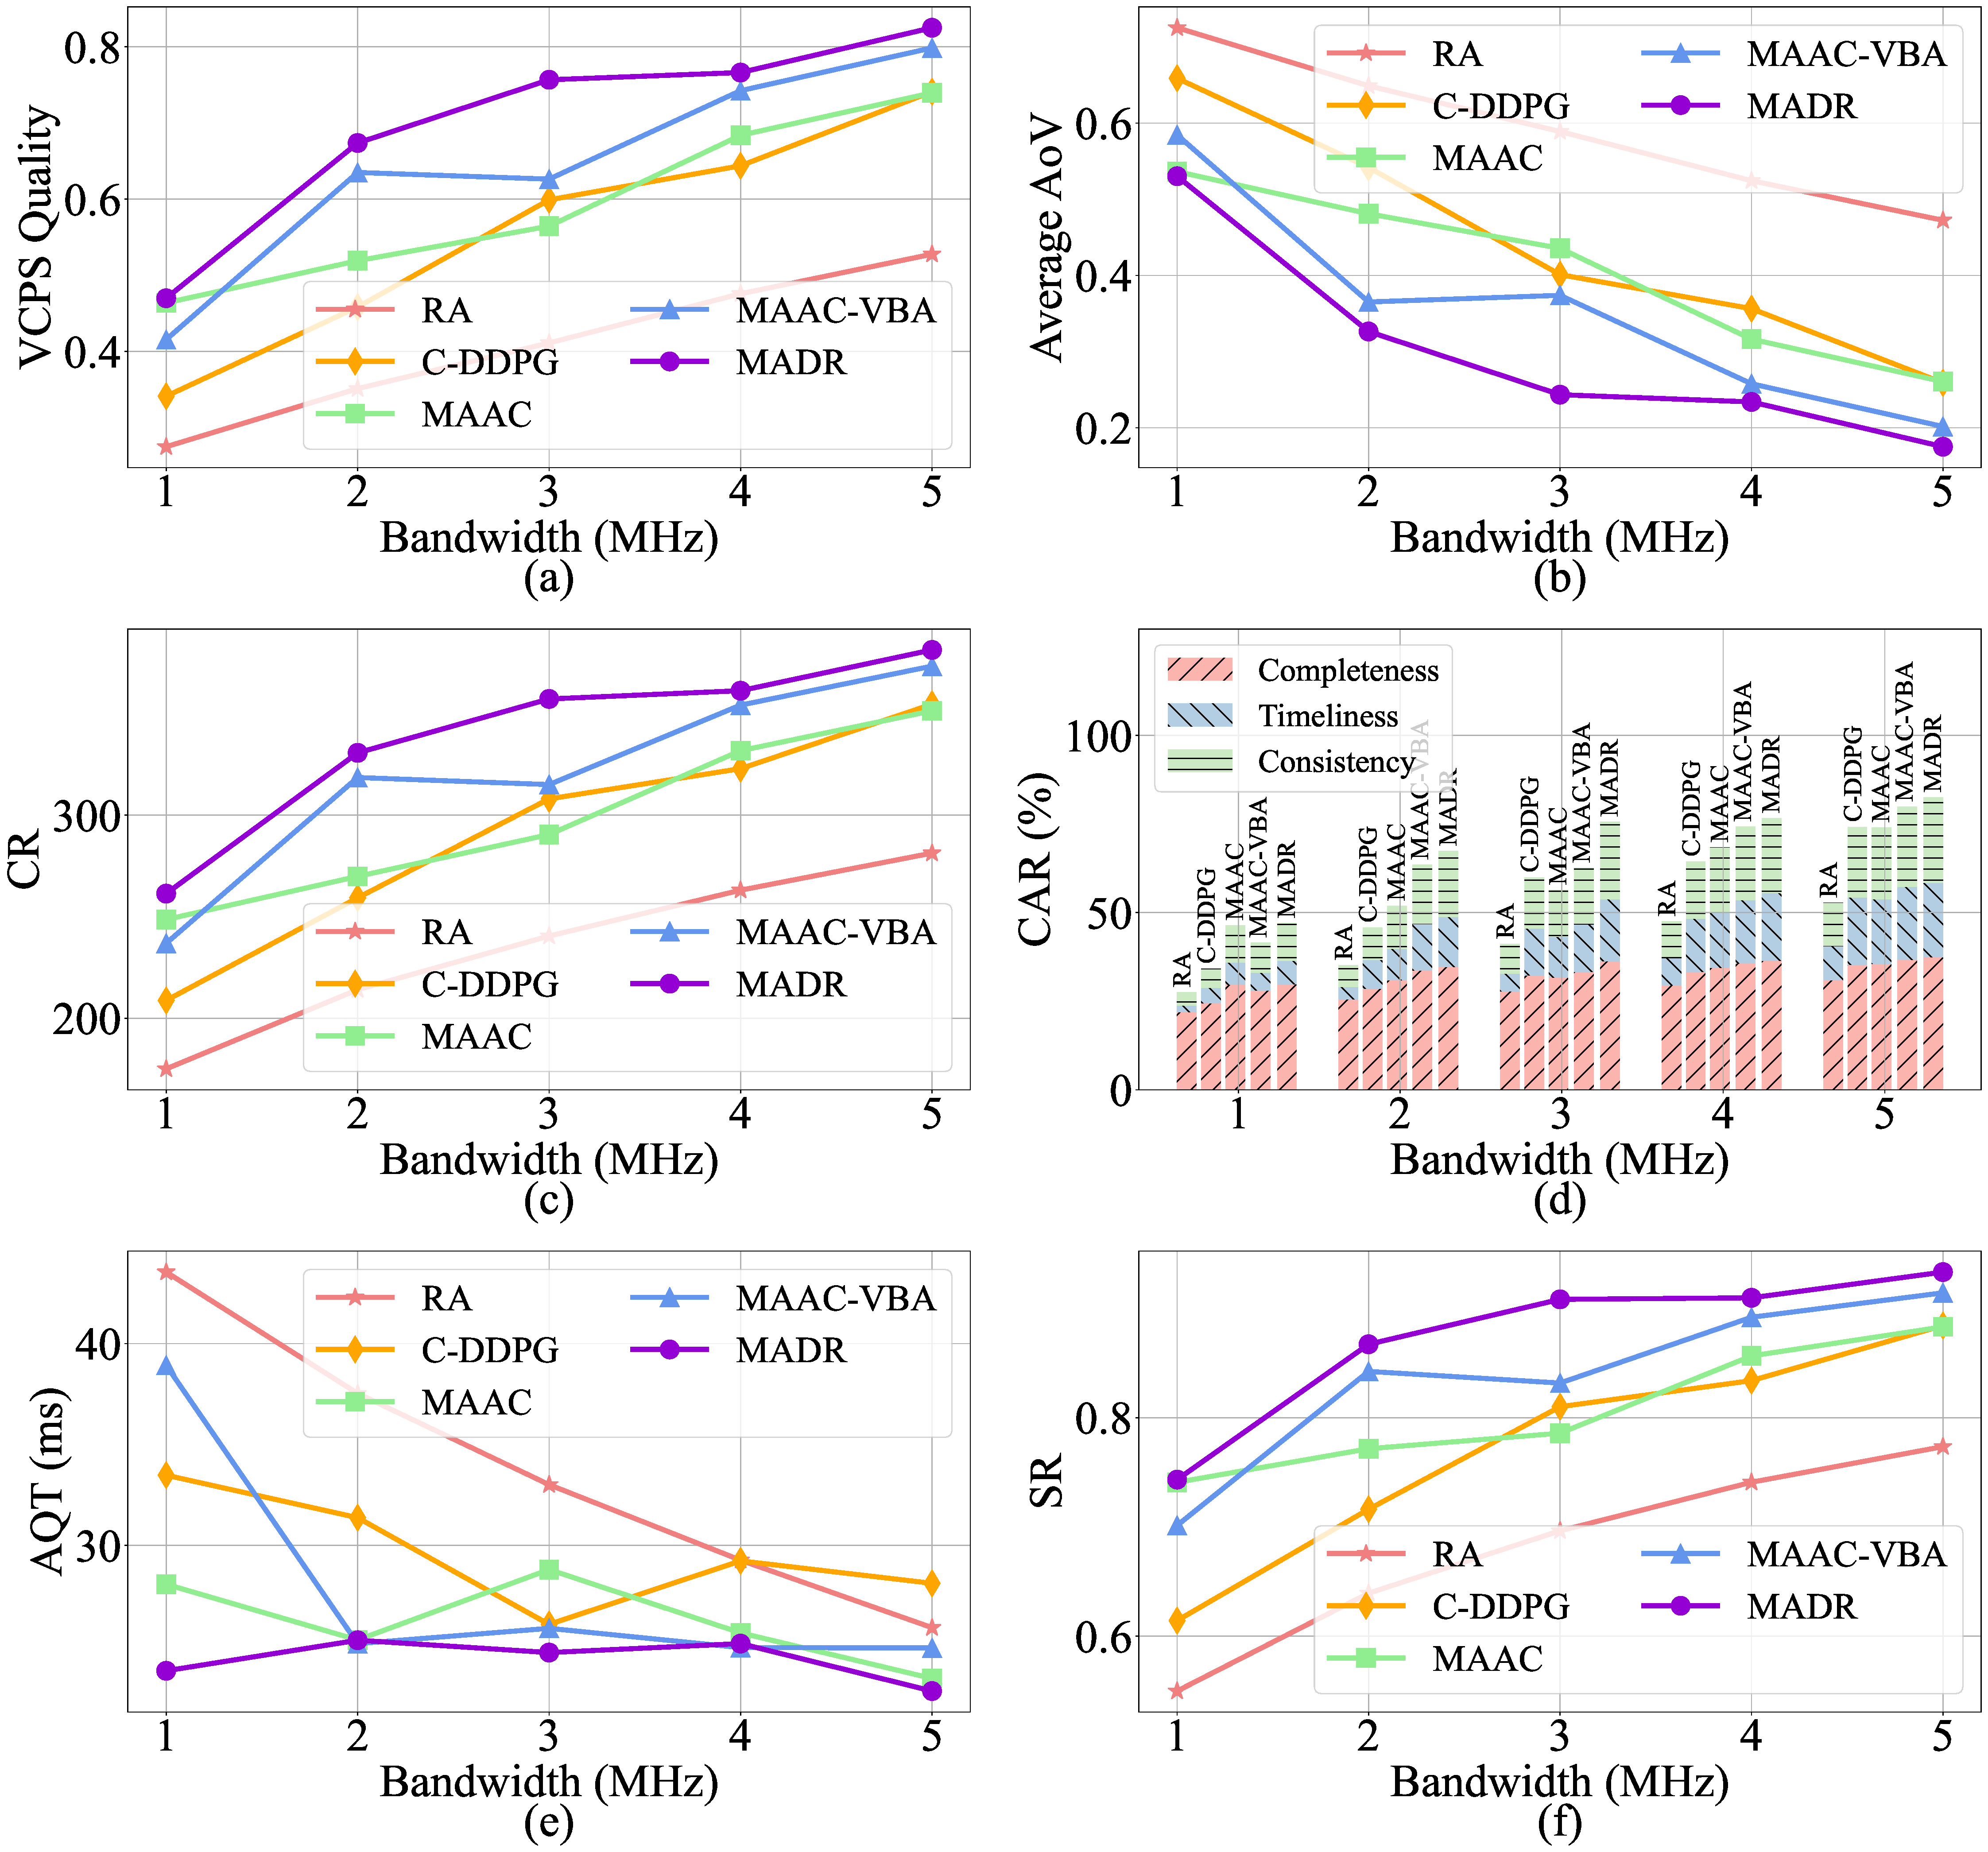
\includegraphics[width=1\columnwidth]{Fig2-8-different-bandwidths.pdf}
  \bicaption[不同V2I带宽下的性能比较]{不同V2I带宽下的性能比较。(a)车载信息物理融合系统质量(b)平均 AoV(c)累积奖励(d)平均奖励的构成(e)平均排队时间(f)服务率}[Performance comparison under different V2I bandwidths]{Performance comparison under different V2I bandwidths. (a) Vehicular cyber-physical system quality (b) Average age of view (c) Cumulative reward (d) Composition of average reward (e) Average queuing time (f) Service ratio}
  \label{fig 2-8}
\end{figure}

\textbf{3) V2I 带宽的影响:}
图\ref{fig 2-8}比较了不同V2I带宽下五种算法的性能。在这组实验中,边缘节点的V2I带宽从1 MHz增加到5 MHz,更大的带宽代表更多的信息可以通过V2I通信上传。图\ref{fig 2-8}(a) 显示了五种算法在VCPS质量方面的比较。随着带宽的增加,所有算法的VCPS质量都相应增加。在不同V2I带宽下,MADR的VCPS质量分别比RA、C-DDPG、MAAC和MAAC-VBA高出约72.9\%、28.3\%、17.8\%和9.3\%。图\ref{fig 2-8}(b) 显示了五种算法在平均AoV方面的比较。所有情况下,MADR实现了最低的平均AoV。图\ref{fig 2-8}(c) 显示了五种算法在CR方面的比较。当带宽增加时,所有五种算法的性能都有所提升。具体来说,相比于RA、C-DDPG、MAAC和MAAC-VBA,MADR在CR方面分别实现了75.1\%、29.4\%、22.7\%和10.6\%的提升。图\ref{fig 2-8}(d) 比较了五种算法在CAR方面的表现。MADR比其他四种算法表现更好,特别是在视图时效性和一致性方面。这是因为在有限的带宽下,所提出的方案中车辆之间的信息感知和上传的协作更加有效。图\ref{fig 2-8}(e) 显示了五种算法在AQT方面的比较。在不同的V2I带宽下,MADR的AQT保持最低,反映了MADR能够更有效地分配带宽。图\ref{fig 2-8}(f) 显示了五种算法在SR方面的比较。在所有情况下,MADR的SR都保持最高水平,进一步证明了MADR在利用有限带宽方面的优势。

\begin{figure}[h]
  \centering
  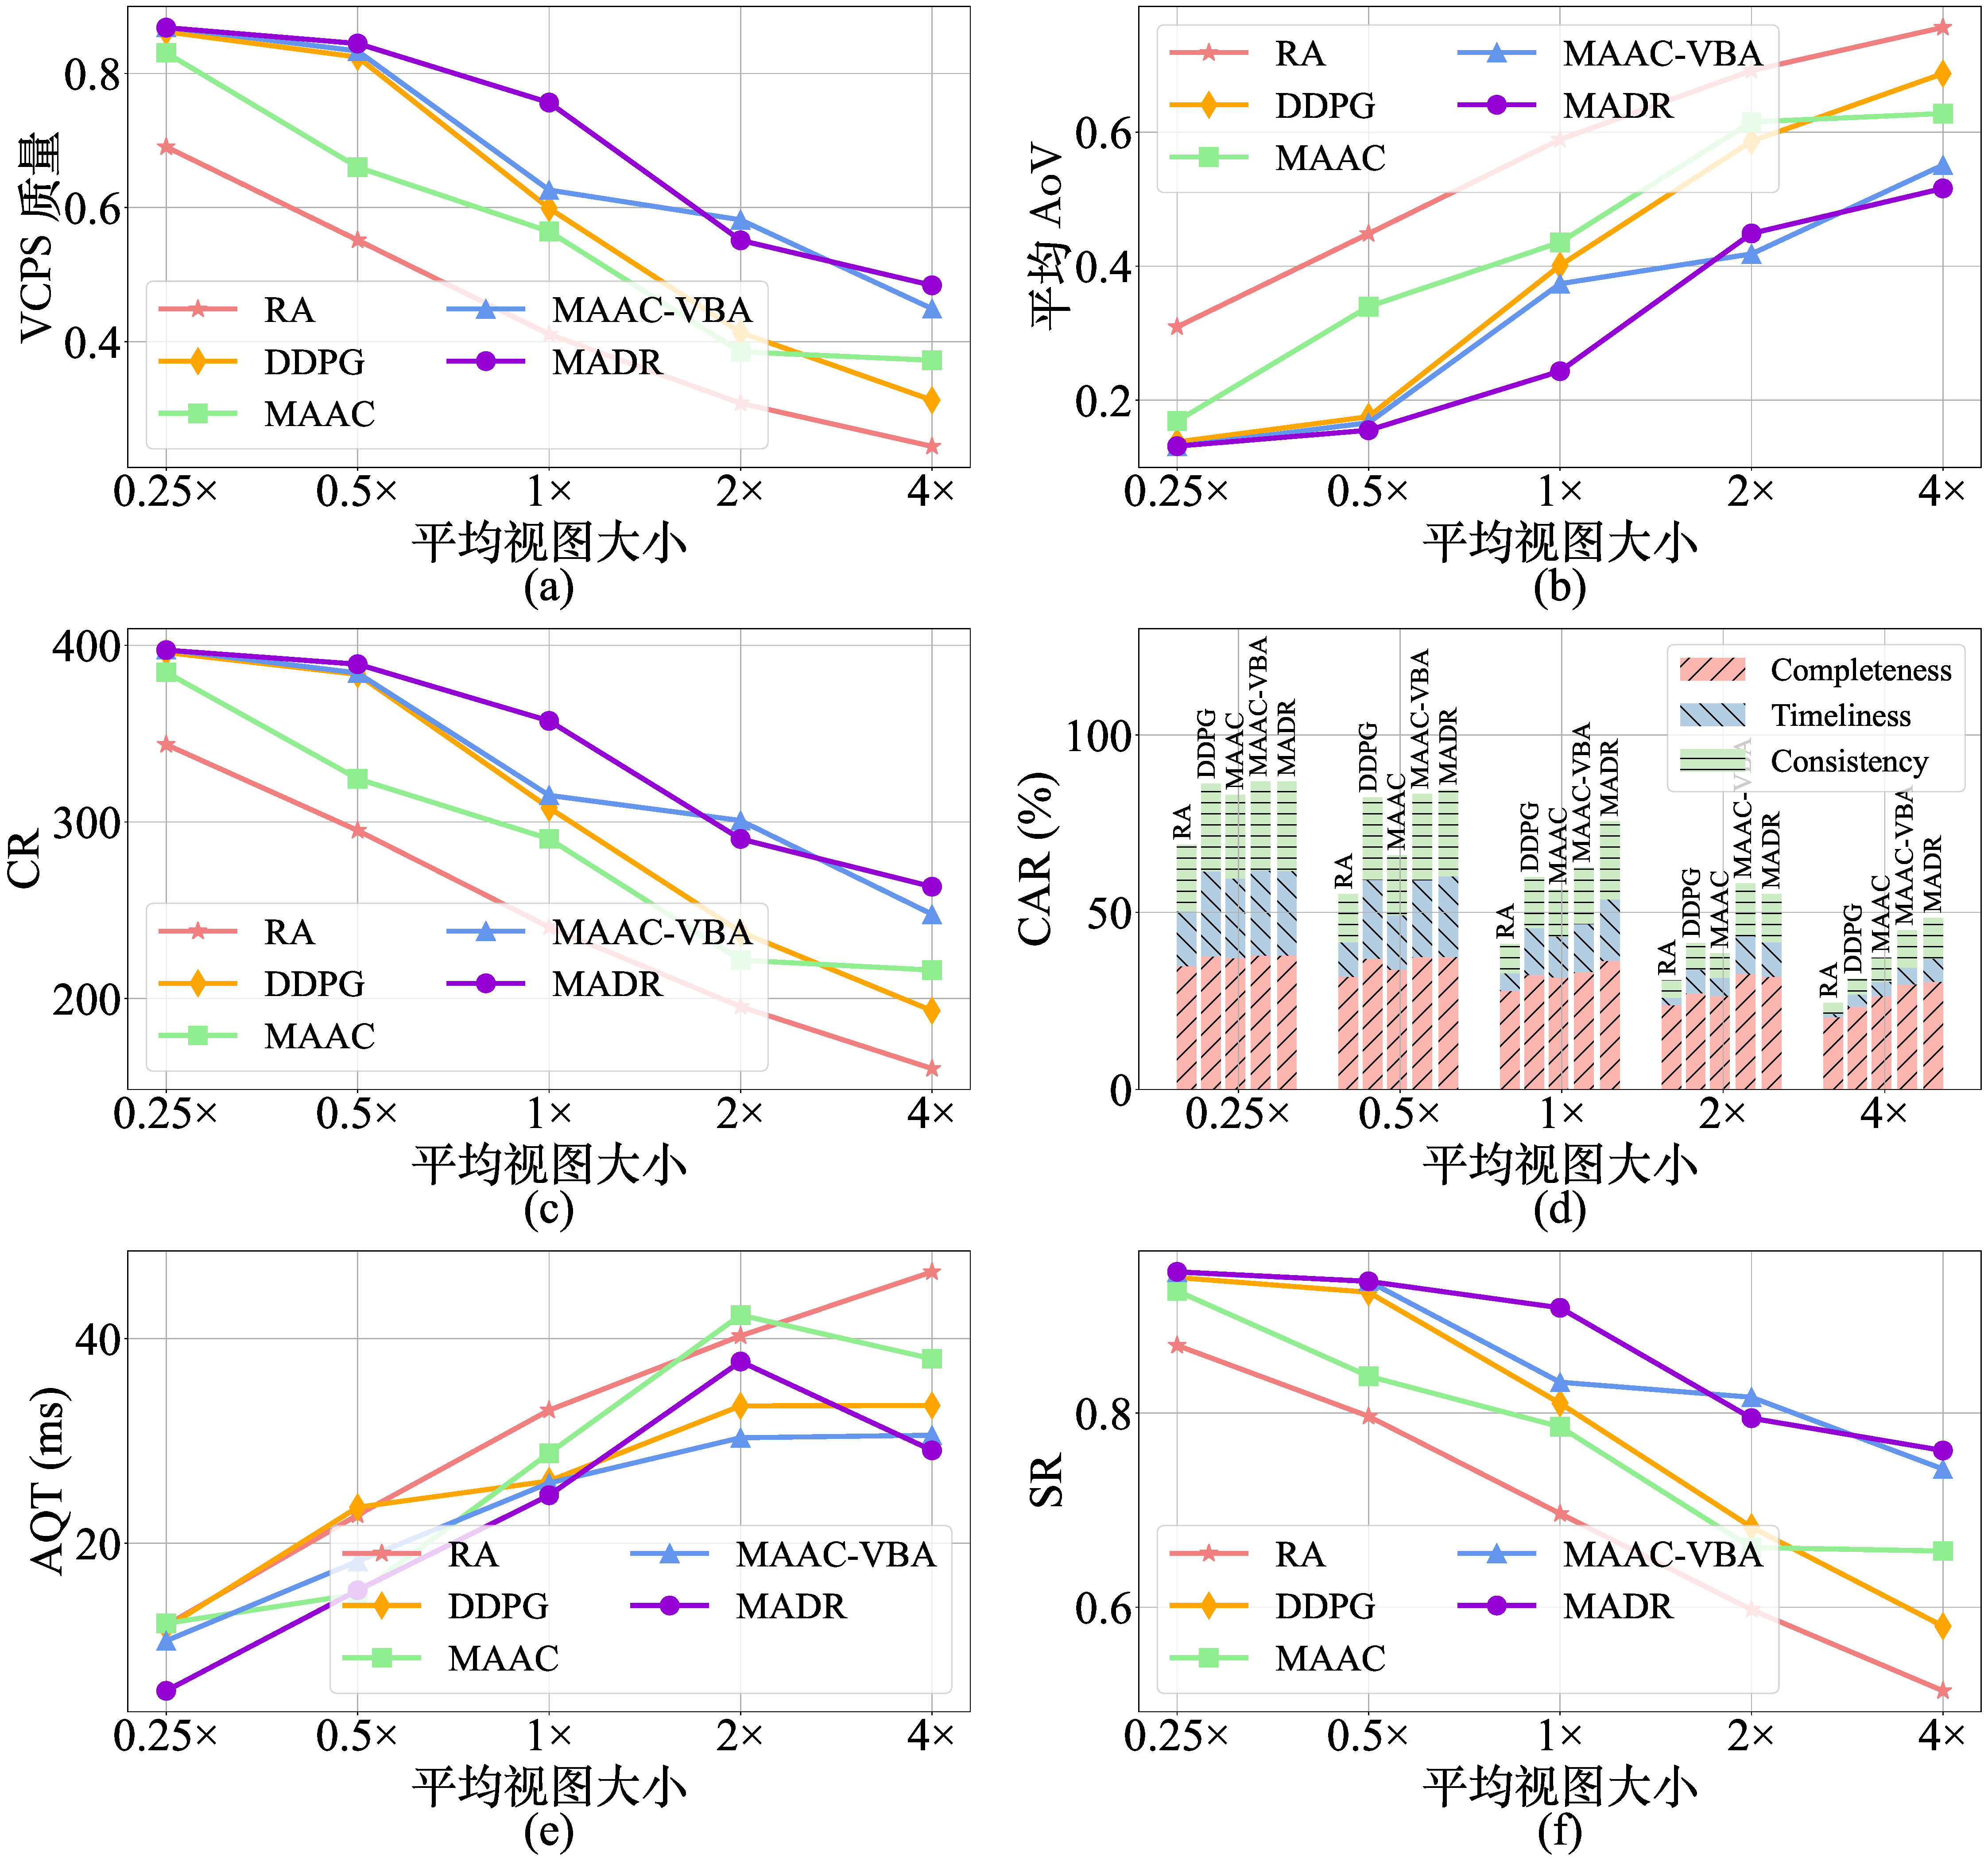
\includegraphics[width=1\columnwidth]{Fig2-9-different-view-sizes.pdf}
  \bicaption[不同视图需求下的性能比较]{不同视图需求下的性能比较。(a)车载信息物理融合系统质量(b)平均 AoV(c)累积奖励(d)平均奖励的构成(e)平均排队时间(f)服务率}[Performance comparison under different requirements on views]{Performance comparison under different requirements on views. (a) Vehicular cyber-physical system quality (b) Average age of view (c) Cumulative reward (d) Composition of average reward (e) Average queuing time (f) Service ratio}
  \label{fig 2-9}
\end{figure}

\textbf{4) 视图需求的影响:}
图\ref{fig 2-9}比较了五种算法在不同视图需求下的性能,其中ITS应用需求的视图平均大小从0.25倍增加到4倍,作为基准,1倍视图的平均大小约为6.46 MB。图\ref{fig 2-9}(a) 显示了五种算法在VCPS质量方面的比较。随着平均视图大小的增加,所有算法的性能都会变差。在不同的视图需求下,MADR在最大限度地提高VCPS质量方面分别比RA、C-DDPG、MAAC和MAAC-VBA高出约68.1\%、23.5\%、27.9\% 和4.9\%。图\ref{fig 2-9}(b)和图\ref{fig 2-9}(c) 比较了五种算法在平均AoV和CR方面的表现。当平均视图大小较小时,MADR中的平均AoV略低于MAAC和MAAC-VBA。MADR、MAAC和MAAC-VBA的CR相似,因为较小的数据量有较高的成功上传的概率。图\ref{fig 2-9}(d) 比较了五种算法在CAR方面的表现。当平均视图大小从0.25倍增加到0.5倍时,MADR和MAAC-VBA之间的性能差异较小,原因是当有足够的资源来满足较小的平均视图大小的要求时,算法的调度效果并不明显。图\ref{fig 2-9}(e) 和图\ref{fig 2-9}(f) 显示了五种算法在AQT和SR方面的比较。结果表明,MADR可以保持最低的AQT,同时在大多数情况下实现最高的SR。当平均视图大小为2倍时,MAAC-VBA实现了最低的AQT和最高的SR,这反映了所提出的VBA方案可以更有效地分配带宽。

\section{本章小结}\label{section 2-7}

本章设计了一个包括应用层、控制层、虚拟层和数据层的车联网分层服务架构,以最大化软件定义网络和移动边缘计算范式的协同效应。
在此基础上,本章提出了分布式感知与异质信息融合场景,并考虑了车载信息物理融合中异质信息的时效性、完整性和一致性,设计了质量指标AoV用于评估边缘构建的逻辑视图。
形式化定义了最大化VCPS质量的问题,并设计了一个基于差分奖励的多智能体深度强化学习解决方案,其中车辆作为独立智能体,决定感知频率和上传优先级。
边缘节点基于车辆预测轨迹和视图需求,通过VBA策略分配V2I带宽。
并采用基于DR的信用分配方案,根据车辆差分奖励评估其对于视图构建的贡献。
通过仿真实验的全面性能评估表明,MADR算法比RA、C-DDPG、MAAC和MAAC-VBA在最大限度地提高VCPS质量方面分别高出约61.8\%、23.8\%、22.0\%和8.0\%,同时加快了收敛速度。
\chapter[面向车载信息物理融合的通信与计算资源协同优化关键技术]{面向车载信息物理融合的通信与计算资源协同优化\\关键技术}
本章将研究面向车载信息物理融合的通信与计算资源协同优化关键技术。
本章内容安排如下:
\ref{section 3-1} 节是本章的引言,介绍车联网中资源分配与任务卸载研究现状、目前研究的不足,以及本章的主要贡献。
\ref{section 3-2} 节阐述了协同通信与计算卸载场景。
\ref{section 3-3} 节形式化定义了协同资源优化问题。
\ref{section 3-4} 节设计了一种基于博弈理论多智能深度强化学习的资源优化策略。
\ref{section 3-5} 节搭建了仿真实验环境并进行了性能验证。
\ref{section 3-6} 节总结本章的研究工作。

\section{引言}\label{section 3-1}

车联网的最新进展为新兴的智能交通系统的发展铺平了道路,例如协同自主驾驶\cite{bagheri20215g}和车载信息物理融合系统\cite{mugabarigira2023context}。
然而,实现车载信息物理融合系统需要大量的数据传输和密集的任务计算。
例如,现代汽车(如特斯拉Model X)已配备了8个摄像头、12个超声波雷达和1个毫米波雷达,其极大增加了感知数据计算的需求。
另一方面,车联网中有限的通信和计算资源使得支持实时 VCPS 构建充满挑战。
因此,研究 VCPS 中高效的实时任务卸载和异构资源分配是当务之急。

车载边缘计算\cite{lang2022cooperative}作为一种有前途的范式出现,以促进车联网边缘的任务处理。
研究人员为VEC的发展付出了巨大的努力 \cite{liu2021fog, dai2021edge, zhang2022digital, liu2020adaptive, liu2018coding},其中边缘节点(如5G基站和路侧设备)搭载计算单元,可以处理车辆通过 V2I 通信上传的数据处理任务。
然而,上述研究都没有利用非正交多址\cite{islam2017power}技术来提高网络容量。
部分研究在车联网中考虑了NOMA\cite{patel2021performance, zhang2021centralized, zhu2021decentralized, liu2019energy},其中车辆可以利用相同频率的频谱资源以不同的传输功率与边缘节点进行通信。
然而,这些研究只考虑了单个边缘节点的情况,不能处理不同边缘节点之间的干扰。
为了提高系统的可靠性,部分研究设计了通信和计算资源的分配机制,以抵消VEC中V2I信道条件和动态可用计算资源的时变影响\cite{liu2021rtds, liu2022a, chen2020robust, liu2014temporal, liu2016cooperative}。
然而,上述研究工作都没有研究实时任务卸载和通信/计算资源分配的协同效应。
一些研究通过整合任务卸载和资源分配制定了联合优化模型 \cite{dai2021asynchronous, dai2022a},但这些研究主要基于集中式调度,这可能会阻碍车联网系统可扩展性。
为解决这个问题,多智能体深度强化学习\cite{kumar2022multi}被提出用于车联网资源优化 \cite{alam2022multi, zhang2021adaptive, nie2021semi}。
另一方面,部分研究结合了强化学习和博弈论 \cite{zheng2022stackelberg, albaba2021driver, rajeswaran2020a}来解决复杂的优化问题。
然而,这些解决方案都不能直接应用于车联网中联合实时任务卸载和异构资源分配。

本章提出了一种基于博弈理论的多智能体深度强化学习的联合任务卸载和资源分配的分布式调度方案。
特别地,本章首先将任务卸载决策过程建模为一个严格势博弈(Exact Potential Game, EPG)\cite{chew2016potential}模型,并证明其在所设计的势函数下具有纳什均衡(Nash Equilibrium, NE)存在性和收敛性。
在该博弈中,边缘节点是理性的玩家,其目标为实现自身利益最大化(最大化实时任务的服务率,即在任务截止时间前完成的任务数占总任务数的比率)。
根据势博弈理论,NE可以基于所设计的势函数最大化每个边缘节点的势来实现。
因此,势博弈中的势函数适合作为所提多智能体分布式深度确定性策略梯度(Multi-Agent Distributed Distributional Deep Deterministic Policy Gradient, MAGT)算法中边缘节点的奖励函数。
然后,本章将资源分配问题分为两个独立的凸优化问题,并提出了一个基于梯度的迭代方法和卡罗需-库恩-塔克(Karush-Kuhn-Tucher, KKT)条件的最优解。

本章对 VCPS 中实时任务卸载和异构资源分配进行了联合研究并解决以下挑战。
首先,V2I上行链路受到使用相同信道的车辆干扰的影响,其影响取决于边缘节点分配的传输功率。
其次,由于计算密集型和延迟敏感型任务的时变分布,不同边缘节点之间的工作负载分配严重失衡。
再次,让边缘节点仅凭其本地知识就能独立有效地决定任务卸载和资源分配的决策是具有挑战性的。
因此,研究联合实时任务卸载和异构资源分配的有效和分布式方法是当务之急,但也具有挑战性。

基于以上分析,本章致力于研究基于NOMA的车载边缘计算中协同资源优化问题,并提出有效分布式算法进行实时任务卸载和异构资源分配。
本章的主要贡献概述如下:
第一,提出了一个基于NOMA的VEC架构,车辆共享相同频率的带宽资源与边缘节点通信,边缘节点为其分配不同的传输功率。
车辆请求具有不同计算资源需求和完成期限的计算任务,其可通过V2I通信上传到边缘节点进行进一步计算。
边缘节点具有异质计算能力,即CPU时钟频率,并选择分配计算资源在本地执行任务,或者通过有线连接将任务迁移到邻近的边缘节点处理。
第二,提出了一个协同资源优化(Cooperative Resource Optimization, CRO)问题,该问题联合卸载任务并分配通信和计算资源以最大化服务率。
具体地,建立了一个V2I传输模型,其中边缘内和边缘间的干扰都是基于NOMA原则来建模的。
然后,通过考虑异构边缘节点的合作,建立了一个任务卸载模型。
第三,提出了基于博弈模型的多智能体深度强化学习来优化通信与计算资源。
具体地,将CRO分解为两个子问题,即任务卸载和资源分配。
将任务卸载子问题建模为边缘节点之间的非合作博弈,并进一步证明其为具有NE存在和收敛性的EPG。
然后,设计了一种MAGT算法,其为D4PG\cite{barth2018distributed}的多智能体版本,以实现纳什均衡,其中边缘节点作为独立的智能体,通过采用实现势作为奖励来评估任务卸载的动作。
此外,将资源分配子问题划分为两个独立的凸问题,并分别通过基于梯度的迭代方法和KKT条件得出最优解。
第四,基于现实世界的车辆轨迹建立了仿真模型,并介绍了除主要指标外的四个指标,包括平均处理时间(Average Processing Time, APT)、平均服务时间(Average Service Time, AST)、平均实现势(Average Achieved Potential, AAP)和本地处理与迁移的比例(Proportion of Locally Processing to Migration, PLPM)。
并实现了所提算法,以及四种有竞争力的解决方案,分别是最优资源分配和任务全迁移(Optimal Resource Allocation and Task Migration Only, ORM)、最优资源分配和任务仅本地处理(Optimal Resource Allocation and Task Local Processing Only, ORL)、分布式深度确定性策略梯度(Distributed Distributional Deterministic Policy Gradient, D4PG)\cite{barth2018distributed},以及多智能体深度确定性策略梯度\cite{zhang2021adaptive},并通过仿真结果证明了所提算法的优越性。

\section{协同通信与计算卸载场景}\label{section 3-2}

本章提出了一个协同通信与计算卸载场景,如图\ref{fig 3-1}所示,沿路安装的基础设施包括5G基站和RSU(如$e_1$$\sim$$e_3$)都安装了不同的计算单元(即CPU芯片),其可作为边缘节点以加速移动车辆卸载的计算任务。
任务随机地到达车辆,其中不同任务可能包含不同的待计算数据。
车辆可以在通信范围内通过V2I通信与边缘节点进行通信。
然后,车辆将任务上传到附近的边缘节点,传输功率由相应的边缘节点分配。
通过在车辆上采用叠加编码(Superposition Coding, SC)技术和在边缘节点上采用串行干扰消除(Successive Interference Cancellation, SIC)\cite{khan2021noma}技术,车辆可以共享同一频率的带宽资源。
在基于NOMA的VEC中,在对弱信号车辆的信号进行解码之前,先由边缘节点对强信号车辆的信号进行解码和消除。
此外,边缘节点之间通过一个有线网络连接。
边缘节点可以决定是否在本地执行收到的任务或通过有线连接将其迁移到其他边缘节点。
最后,边缘节点为需要处理的任务分配计算资源。

\begin{figure}[h]
\centering
  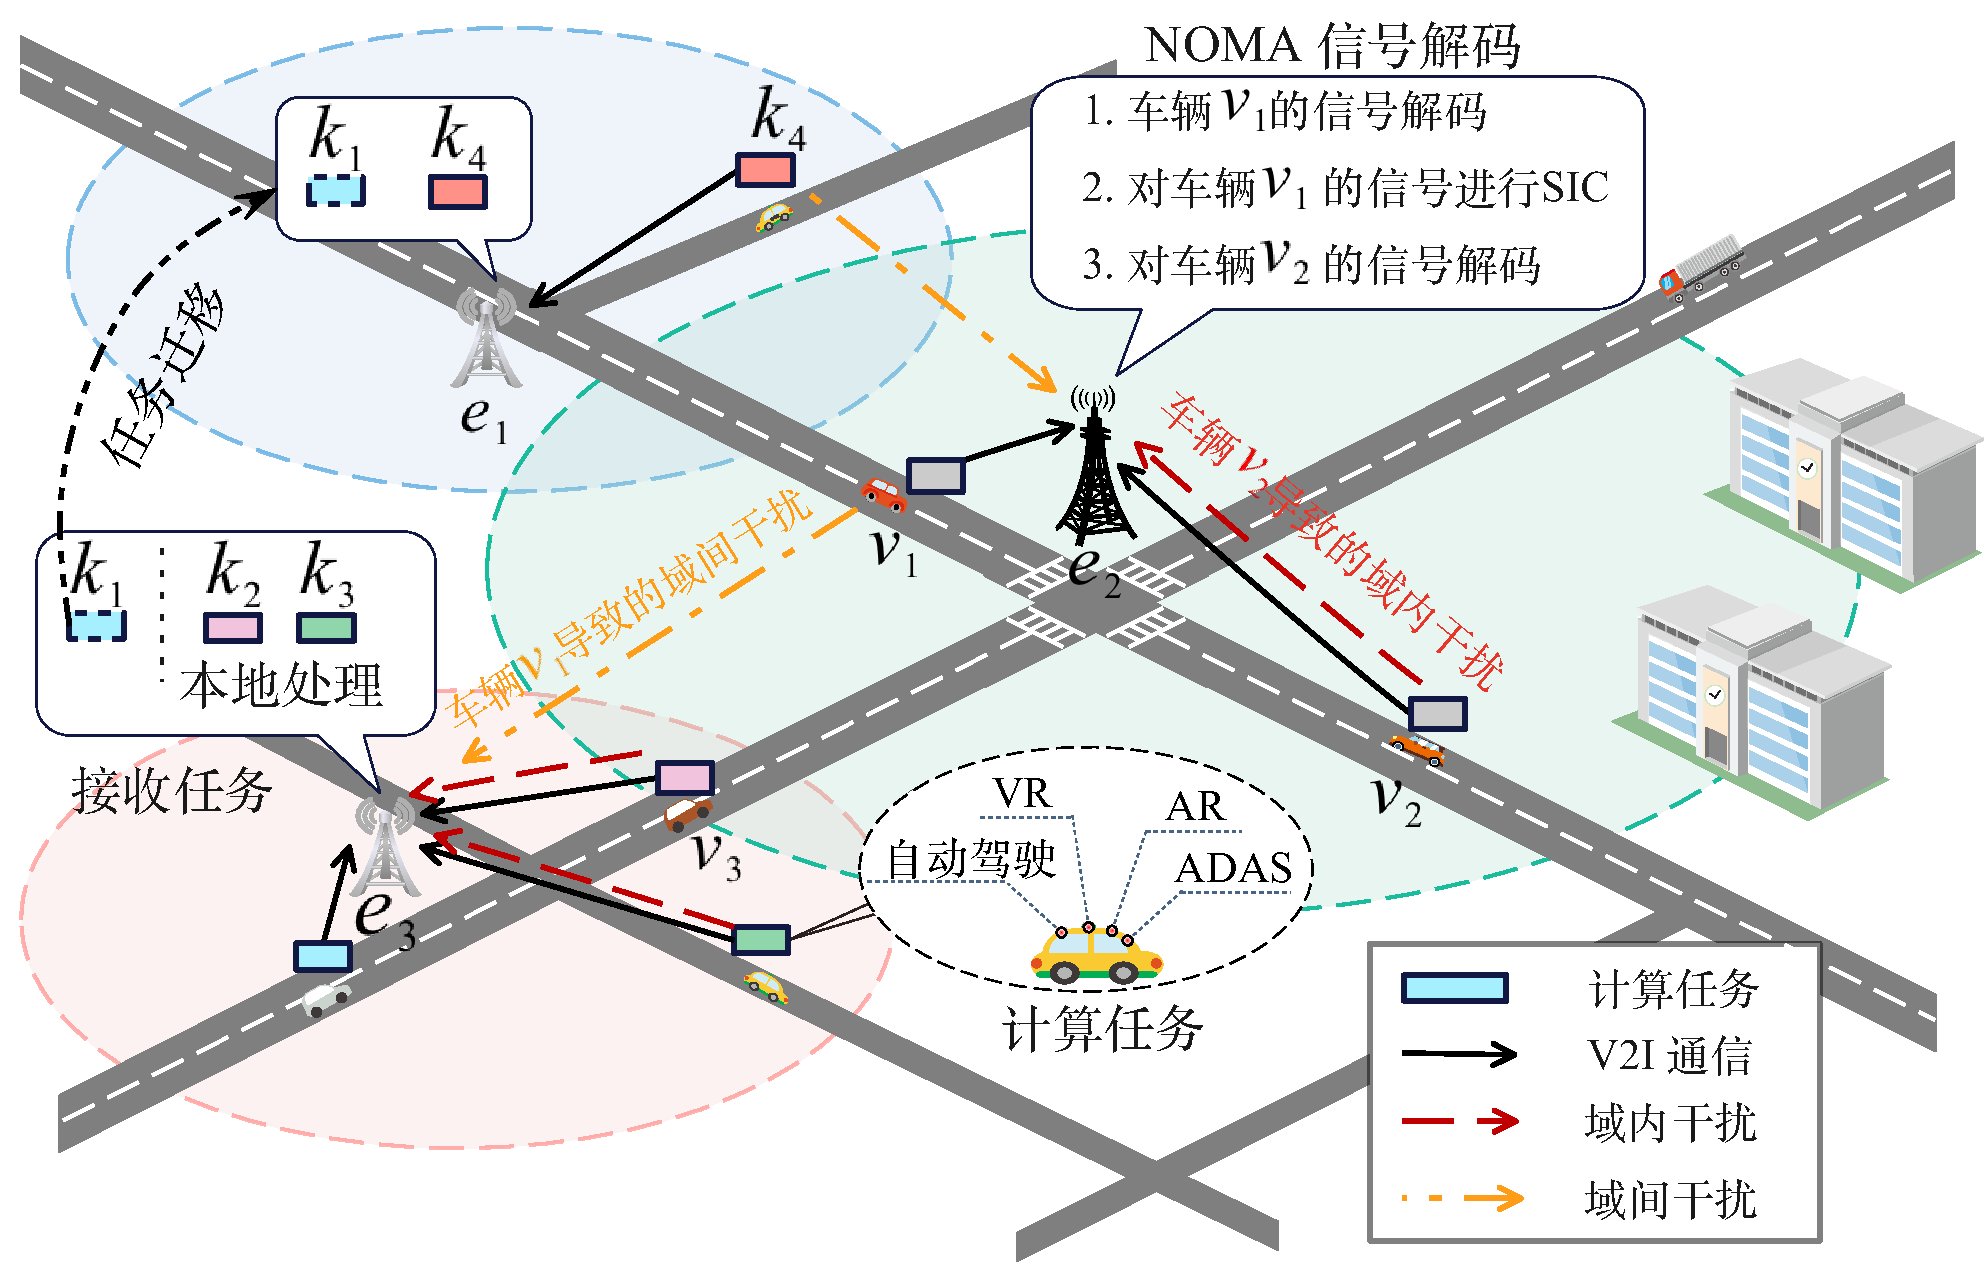
\includegraphics[width=1\columnwidth]{Fig4-1-noma-architecture.pdf}
  \bicaption{协同通信与计算卸载场景}{Cooperative transmission and computation offloading scenario}
  \label{fig 3-1}
\end{figure} 

本系统的特点总结如下:
首先,车辆请求的计算任务可能有不同的数据大小、计算资源要求和截止时间。
因此,任务完成情况(即任务是否能在最后期限前成功完成)当被卸载到具有不同计算能力(即CPU时钟频率)的边缘节点时可能有所不同。
其次,增加车辆的传输功率虽然可能会提高V2I传输率,但是也会由于边缘内和边缘间的干扰增强而损害其他V2I上行链路。
此外,边缘节点的功率分配随着时间的推移而变化,并且相互之间是未知的。
因此,边缘节点必须通过考虑其他边缘节点的功率分配的影响来确定车辆的传输功率。
最后,由于任务的随机到达和车辆的时变分布,边缘节点的工作负载可能不平衡。
当一个边缘节点负担过重时,将额外的任务迁移到其他有多余计算资源的边缘节点以加快处理是合适的。
然而,通过有线连接将任务数据传输到边缘节点也会延长任务服务时间。

进一步,本章提供一个例子来更好地说明上述问题。
如图\ref{fig 3-1}所示,车辆$v_1$和$v_2$通过V2I通信上传计算任务。
由于边缘节点$e_2$和车辆$v_1$之间的V2I信道条件优于车辆$v_2$和$v_3$,车辆$v_1$的信号可以通过将其他信号视为噪声来进行优先解码。
然后,在对车辆$v_2$和$v_3$的信号进行解码时,车辆$v_1$的信号可以被边缘节点$e_2$通过SIC进行消除。
然而,车辆$v_1$的信号在V2I传输过程中可能受到车辆$v_2$的干扰;这种干扰被称为“边缘内干扰”,因为车辆$v_1$和$v_2$处于同一个边缘节点$e_2$的无线电覆盖范围内。
另一方面,车辆$v_3$的信号可能受到车辆$v_1$的干扰,这种来自其他边缘节点的干扰被称为“边缘间干扰”。
此外,很明显,边缘节点$e_1$和$e_3$之间的任务负载是不均匀的,因为在边缘节点$e_3$中有三个任务(即$k_1$、$k_2$和$k_3$),但在边缘节点$e_1$中只有一个任务$k_4$。
假设边缘节点$e_1$的计算资源明显多于边缘节点$e_3$的资源,那么任务$k_1$应该通过有线网络迁移到边缘节点$e_1$,因而可以在更短的时间内得到服务。
如上所述,通过设计一个有效的分布式调度机制来实现实时任务卸载和异构资源分配,从而优化系统的整体性能,这对利用边缘节点之间的协作通信和计算是非常关键且具有挑战性的。

\section{协同资源优化问题定义}\label{section 3-3}

离散时间片的集合用$\mathbf{T}=\{1, \ldots, t, \ldots, T\}$表示,其中$T$是时间片的数量。
车辆的集合用$\mathbf{V}=\{1, \ldots, v, \ldots, V\}$表示,车辆$v \in \mathbf{V}$在$t$时的位置用$l_{v}^{t}$表示。
车辆$v$在时间$t$的任务到达概率用$\tau_{v}^{t}$表示,并用$\mathbf{K}_{v}$表示车辆$v$请求的任务集合。
车辆$v$在时间$t$要求的任务$k_{v}^{t} \in \mathbf{K}_{v}$由三元组表示$k_{v}^{t}=\left(d_{k}, c_{k}, t_{k}\right)$,其中$d_{k}$、$c_{k}$和$t_{k}$分别为数据大小、处理一位数据的CPU周期和任务处理截止时间。
边缘节点的集合用$\mathbf{E}=\{1, \ldots, e, \ldots, E\}$表示,边缘节点$e \in \mathbf{E}$由四元组$e=\left(p_{e}, c_{e}, g_{e}, l_{e}\right)$表示,其中$p_{e}$是V2I通信的最大功率,$c_{e}$是计算频率,$g_e$是V2I通信范围,$l_{e}$是位置。
边缘节点之间有线通信的传输速率用$z$表示。
车辆$v$与边缘节点$e$在时间$t$的距离用$\operatorname{dis}_{v, e}^{t}$表示。
在$t$时间,在边缘节点$e$的无线电覆盖范围内的车辆集合用$\mathbf{V}_{e}^{t}=\left\{v \mid \operatorname{dis}_{v, e}^{t} \leq g_{e}, \forall v \in \mathbf{V}\right\}, \mathbf{V}_{e}^{t} \subseteq \mathbf{V}$表示。
V2I通信的带宽用$b$表示。

\begin{figure}[h]
\centering
  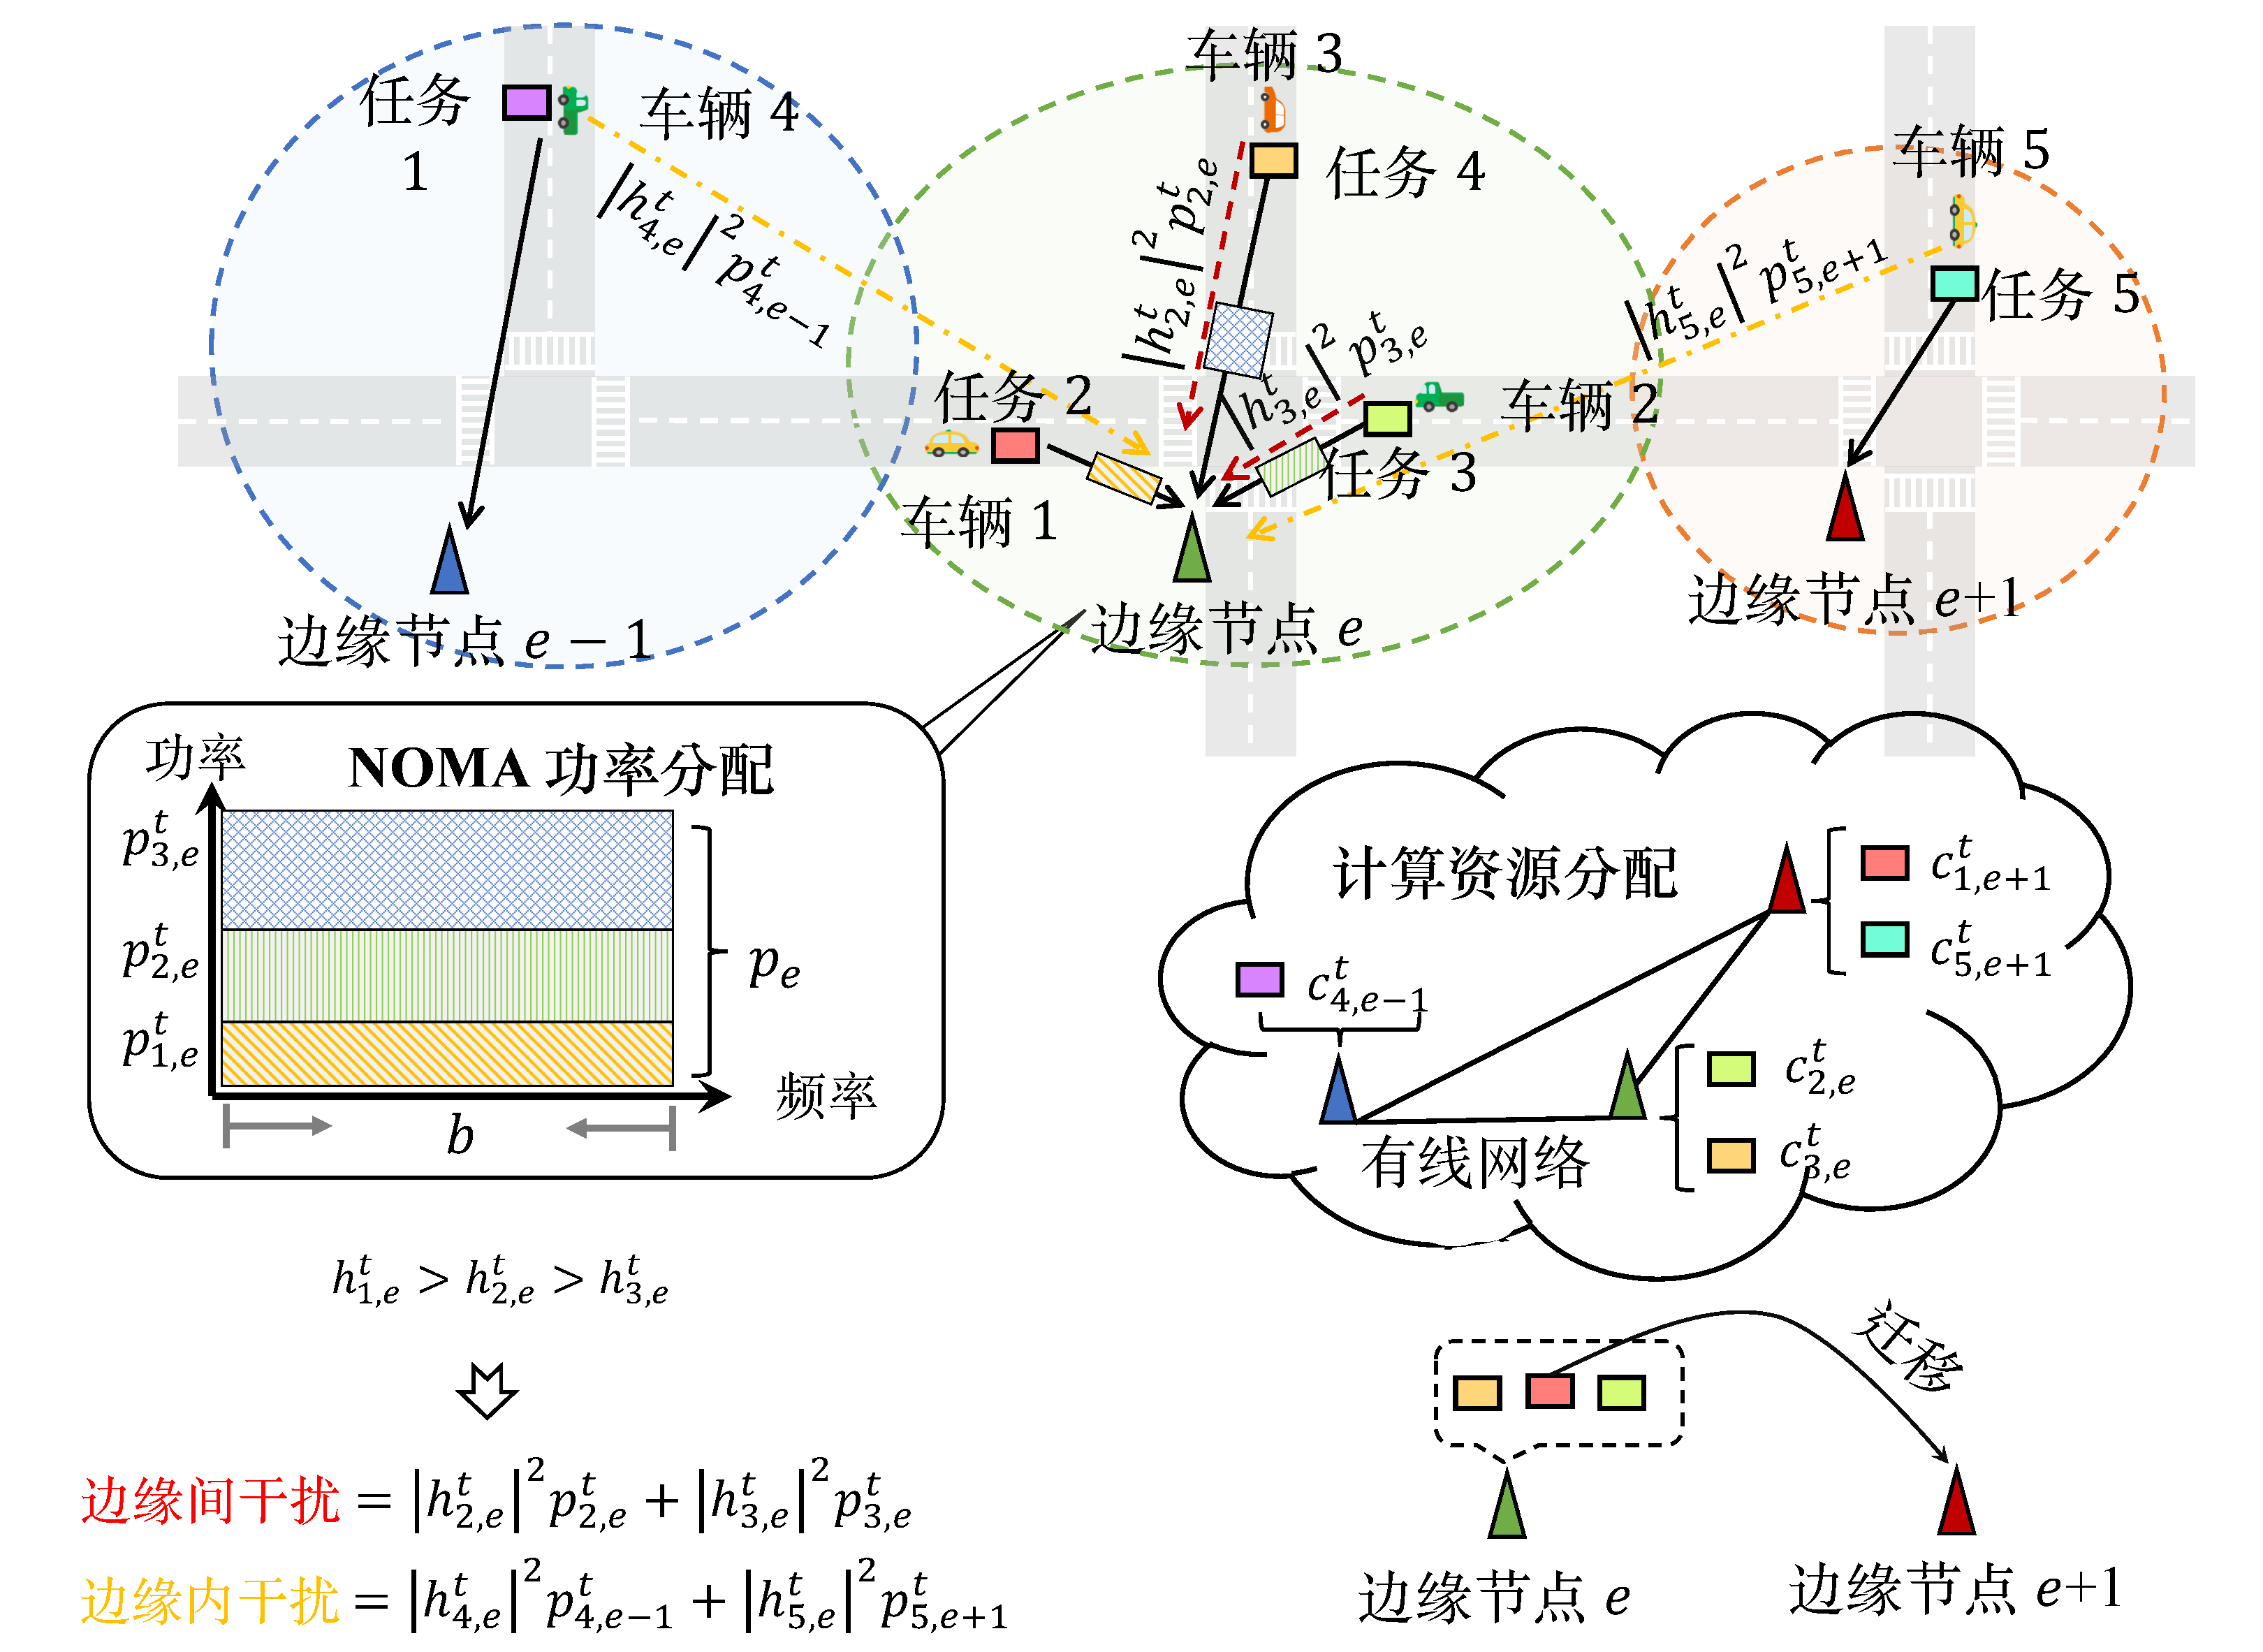
\includegraphics[width=1\columnwidth]{Fig4-2-system-model.pdf}
  \bicaption{V2I 传输与任务卸载模型}{V2I transmission and task offloading model}
  \label{fig 3-2}
\end{figure}

\subsection{V2I 传输模型}

本章节构建了V2I传输模型,如图\ref{fig 3-2}所示, 其中边缘内和边缘间干扰的干扰是基于NOMA原则建模的。
本章将边缘节点$e$在时间$t$分配的车辆$v$的传输功率表示为$p_{v, e}^{t}$。
分配的功率之和不能超过边缘节点$e$的V2I通信的最大功率,即$\sum_{\forall v \in {V}_{e}^{t}} p_{v, e}^{t} \leq p_{e}$。
然后,车辆$v$和边缘节点$e$之间在时间$t$的信道增益用$h_{v, e}^t$表示,可通过以下公式计算\cite{sun2020performance}
\begin{equation}
	h_{v, e}^t = \frac{\eta_{v, e}}{{\operatorname{dis}_{v, e}^{t}}^{\varphi/2}}
\end{equation}
\noindent 其中$\eta_{v, e}$是瑞利分布的小尺度衰减,即$\eta_{v, e} \sim \mathcal{CN}(0, 1)$,$\varphi$是大尺度路径损耗指数。
因此,比车辆$v$的瞬时信道条件更差的车辆集合用$\mathbf{V}_{h_{v, e}}^{t}$表示,其表示为
\begin{equation}
	\mathbf{V}_{h_{v, e}}^{t} = \left \{ v^{\prime} \mid  \left|h_{v^{\prime}, e}^t \right|^{2} < \left| h_{v, e}^t\right |^{2} , \forall v^{\prime} \in \mathbf{V}_{e}^{t} \right \}
\end{equation}
在确定了每个车辆$v \in \mathbf{V}_{e}^{t}$的传输功率后,边缘节点$e$的观测信号可以表示为\cite{islam2017power}
\begin{equation}
	y_e^{t} = \sum_{\forall v \in \mathbf{V}_{e}^{t}} p_{v, e}^{t} s_{v, e}^{t} h_{v, e}^t + \sum\limits_{\forall e^{\prime} \in \mathbf{E} / \{e\}} \sum\limits_{\forall v^{\prime} \in \mathbf{V}_{e^{\prime}}^{t}} p_{v^{\prime}, e^{\prime}}^{t} s_{v^{\prime}, e^{\prime}}^{t} h_{v^{\prime}, e}^t + N_{0}
\end{equation}
其中$s_{v, e}^{t}$是用于车辆$v$的信息,$N_{0}$是AWGN。
根据NOMA原则,边缘节点$e$可以通过SIC消除信道条件比车辆$v$好的车辆的信号 \cite{du2021ji}。
因此,车辆$v$和边缘节点$e$之间在时间$t$的信号与干扰加噪声比(Signal-to-Interference-plus-Noise Ratio, SINR)用$\mathrm{SINR}_{v, e}^t$表示,可以通过以下公式计算
\begin{equation}
	\mathrm{SINR}_{v, e}^t = \frac{ |h_{v, e}^t| ^{2}  p_{v, e}^{t}}{ \underbrace{\sum\limits_{\forall v^{\prime} \in \mathbf{V}_{h_{v, e}}^{t}} |h_{v^{\prime}, e}^t|^2 p_{v^{\prime}, e}^{t}}_{\text {边缘内干扰}} + \underbrace{\sum\limits_{\forall e^{\prime} \in \mathbf{E} / \{e\}} \sum\limits_{\forall v^{\prime} \in \mathbf{V}_{e^{\prime}}^{t}} |h_{v^{\prime}, e}^t|^2 p_{v^{\prime}, e^{\prime}}^{t}}_{\text {边缘间干扰}} + N_{0}}
\end{equation}
其中$p_{v^{\prime}, e}^{t}$是车辆$v^{\prime} \in \mathbf{V}_{e}^{t}$的传输功率,$|h_{v^{\prime}, e}^t|^2$是车辆$v^{\prime}$与边缘节点$e$之间干扰环节的信道系数。
分母中的第一和第二部分分别代表边缘内和边缘间干扰。
因此,由车辆$v$请求并传输给边缘节点$e$的任务$k_{v}^{t}$的上传时间由以下方式计算
\begin{equation}
	m_{v, e}^{t} = \frac{d_{k}}{b  \log _{2}\left(1+\mathrm{SINR}_{v, e}^t\right)}
\end{equation}
其中$d_k$是任务$k_{v}^{t}$的数据大小,$b$是V2I通信的带宽。

\subsection{任务卸载模型}
边缘节点$e$在时间$t$的覆盖范围内的车辆上传的任务集合用$\mathbf{K}_{e}^{t} = \{ k_{v}^{t}| \forall v \in \mathbf{V}_{e}^{t} \}$表示。 
如图\ref{fig 3-2}所示,每个任务$k_{v}^{t} \in \mathbf{K}_{e}^{t}$都可以在本地的边缘节点$e$中执行,或者迁移到其他边缘节点进行处理。
任务卸载指示器用$q_{v, e}^{t}$表示,其表示车辆$v$的任务$k_{v}^{t}$在时间$t$是否被卸载到边缘节点$e$。
每个任务至多只能卸载到一个边缘节点,即$\sum_{\forall e \in \mathbf{E}} q_{v, e}^{t} = 1$。
那么,在边缘节点$e$中卸载的任务集可以用以下式表示
\begin{equation}
	\mathbf{K}_{q_e}^{t} = \left\{ k_{v}^{t} | q_{v, e}^{t} = 1, \forall v \in \mathbf{V}_{e^{\prime}}^{t}, \forall e^{\prime} \in \mathbf{E} \right\}
\end{equation}
其中包括车辆上传的本地处理任务和从其他边缘节点迁移的任务。
由边缘节点$e$分配任务$k_{v}^{t} \in \mathbf{K}_{q_e}^{t}$的计算资源(即CPU时钟频率)用$c_{v, e}^{t}$表示。
整体分配的计算资源不能超过边缘节点$e$的计算能力,即 $ \sum_{\forall k_{v}^{t} \in {\mathbf{K}_{q_e}^{t} }} c_{v, e}^t \leq c_{e}$,其中$c_e$是边缘节点$e$的CPU时钟频率。
因此,任务$a_{v}^{t}$在边缘节点$e$中的执行时间用$x_{v, e}^t$表示,其计算公式为
\begin{equation}
	x_{v, e}^t = \frac{ d_{k}  c_{k}}{c_{v, e}^t}
\end{equation}
其中$d_{k}$是任务$k_{v}^{t}$的大小,$c_{k}$是处理任务$k_{v}^{t}$中1 bit 数据的CPU周期。

然而,当车辆$v$请求任务$k_{v}^{t}$时,车辆$v$可能不在边缘节点$e$的无线电覆盖范围内,因而任务$k_{v}^{t}$不能被执行,直到全部任务数据被卸载边缘节点$e$收到。
因此,本章用$w_{v, e}^{t}$表示由边缘节点$e$传输并在边缘节点$e^{\prime}$接收的任务$k_{v}^{t}$的有线传输时间,其计算公式为
\begin{numcases}{w_{v, e}^{t} =}
0, &$k_{v}^{t} \in \mathbf{K}_{e}^{t} \bigcap \mathbf{K}_{q_e}^{t}$ \notag \\
{d_{k}  \operatorname{dis}_{e, e^{\prime}}^{t}}  \zeta  / {z},  &$k_{v}^{t} \in \mathbf{K}_{e}^{t} \bigcap \mathbf{K}_{q_{e^{\prime}}}^{t}$
\end{numcases}
\noindent 其中$\operatorname{dis}_{e, e^{\prime}} ^{t}$是边缘节点$e$和$e^{\prime}$之间的距离,$\zeta$是一个距离折扣常数。
任务$k_{v}^{t}$在边缘节点$e$中的处理时间用$n_{v, e}^t$表示,用以下公式表示
\begin{equation}
n_{v, e}^t= w_{v, e}^{t} + \sum_{\forall e^{\prime} \in \mathbf{E}} q_{v, e^{\prime}}^{t} x_{v, e^{\prime}}^t
\label{equ 3-9}
\end{equation}
任务$k_{v}^{t}$的处理时间由有线传输时间和执行时间组成,其取决于任务卸载决策。

\subsection{协同资源优化问题}

任务$k_v^t \in \mathbf{K}_{e}^{t}$的服务时间由上传时间和处理时间组成,用$\psi_{v, e}^{t}$表示
\begin{equation}
	\psi_{v, e}^{t} = m_{v, e}^{t} +  n_{v, e}^{t}
	\label{equ 3-10}
\end{equation}
只有当服务时间短于任务截止时间$t_k$时,任务$k_v^t$才能成功服务。
那么,边缘节点$e$的服务率可定义为成功服务的任务数(即在任务截止时间前被服务)与边缘节点$e$的请求任务数之间的比率,用$\Psi_{e}^{t}$表示,并通过以下方式表示
\begin{equation}
	\Psi_{e}^{t} = \frac{\sum_{\forall k_{v}^{t} \in \mathbf{K}_{e}^{t}} \mathbb{I} \left\{ \psi_{v, e}^{t} \leq t_{k} \right\} }{|\mathbf{K}_{e}^{t}|}
	\label{equ 3-11}
\end{equation}
\noindent 其中,$|\mathbf{K}_{e}^{t}|$ 是边缘节点$e$覆盖范围内的车辆请求的任务数,$\mathbb{I} \left\{ \psi_{v, e}^{t} \leq t_{k} \right\}$是一个指示函数,即如果 $\psi_{v, e}^{t} \leq t_{k}$,则$\mathbb{I} \left\{ \psi_{v, e}^{t} \leq t_{k} \right\} =1$,否则,$\mathbb{I} \left\{ \psi_{v, e}^{t} \leq t_{k} \right\} =0$。

给定一个确定的解决方案$(\mathbf{P}, \mathbf{Q}, \mathbf{C})$,其中$\mathbf{P}$表示确定的V2I传输功率分配,$\mathbf{Q}$表示确定的任务卸载决策,$\mathbf{C}$表示确定的计算资源分配,其表示为
\begin{numcases}{}
	\mathbf{P}= \left \{ p_{v, e}^{t} \mid \forall v \in \mathbf{V}_{e}^t, \forall e \in \mathbf{E}, \forall t \in \mathbf{T}\right \} \notag \\
	\mathbf{Q}= \left \{ q_{v, e}^t \mid \forall v \in \mathbf{V}, \forall e \in \mathbf{E}, \forall t \in \mathbf{T} \right \} \notag \\ 
	\mathbf{C}= \left \{ c_{v, e}^t \mid \forall v \in \mathbf{V}, \forall e \in \mathbf{E}, \forall t \in \mathbf{T} \right \}
\end{numcases}
本章旨在通过联合优化基于NOMA的VEC中的任务卸载决策和异构资源分配,实现调度期间边缘节点服务率之和的最大化。
因此,协作资源优化问题表述如下:
\begin{align}
	\operatorname{CRO}:&\max_{\mathbf{P}, \mathbf{Q}, \mathbf{C}} f_1= \sum_{\forall t \in \mathbf{T}} \sum_{ \forall e \in \mathbf{E}} \Psi_{e}^{t} \notag \\
		\text { s.t. }
    &\mathcal{C}3.1: \sum_{\forall v \in \mathbf{V}_{e}^{t}} p_{v, e}^{t} \leq p_{e}, \forall e \in \mathbf{E}, \forall t \in \mathbf{T} \notag \\
    &\mathcal{C}3.2: \sum_{\forall k_{v}^{t} \in {\mathbf{K}_{q_e}^{t} }} c_{v, e}^t \leq c_{e}, \forall e \in \mathbf{E}, \forall t \in \mathbf{T} \notag \\
   	&\mathcal{C}3.3: q_{v, e}^t \in \left \{0, 1\right \}, \forall v \in \mathbf{V}, \forall e \in \mathbf{E}, \forall t \in \mathbf{T}  \notag \\
    &\mathcal{C}3.4: \sum_{\forall e \in \mathbf{E}} q_{v, e}^t = 1, \forall v \in \mathbf{V}, \forall t \in \mathbf{T} 
\end{align}
其中约束条件$\mathcal{C}3.1$保证边缘节点分配的总传输功率不能超过V2I通信的最大功率。
$\mathcal{C}3.2$要求分配的总体计算资源不能超过边缘节点的计算能力。
约束条件 $\mathcal{C}3.3$ 和 $\mathcal{C}3.4$ 规定任务卸载决策 $q_{v, e}^t$ 是一个 0-1 的整数变量,且每个任务只能卸载到一个边缘节点。

\section{基于博弈理论的多智能体强化学习算法设计}\label{section 3-4}

本章节提出了基于博弈理论的多智能体强化学习算法,如图\ref{fig 3-3}所示,通过解耦CRO,其可被分解为两个独立子问题来解决,即任务卸载($\mathcal{P}3.1$)和资源分配($\mathcal{P}3.2$)。
特别地,$\mathcal{P}3.1$被建模为边缘节点之间的非合作博弈,并被证明为具有NE存在和收敛性的EPG。
为了解决$\mathcal{P}3.1$,本章设计了在每个边缘节点实现的MAGT,用于任务卸载以实现NE。
另一方面,$\mathcal{P}3.2$被分解为两个独立的凸优化问题。
本章分别通过基于梯度的迭代方法和KKT条件,推导出解决$\mathcal{P}3.2$异构资源分配的最优解。
两个子问题解决方案之间的交互描述如下:
首先,任务卸载决策是基于MAGT和本地系统观察的输入提前确定的。
然后,根据任务卸载决策,通过最优方案获得资源分配。
此外,在基于NOMA的VEC环境中,利用任务卸载和资源分配的联合动作,通过设计的势能函数获得边缘节点的奖励。
上述过程将持续到MAGT的训练完成。
基于博弈理论的多智能体强化学习算法的详细步骤见算法\ref{algorithm 3-1}。

\begin{figure}[h]
\centering
  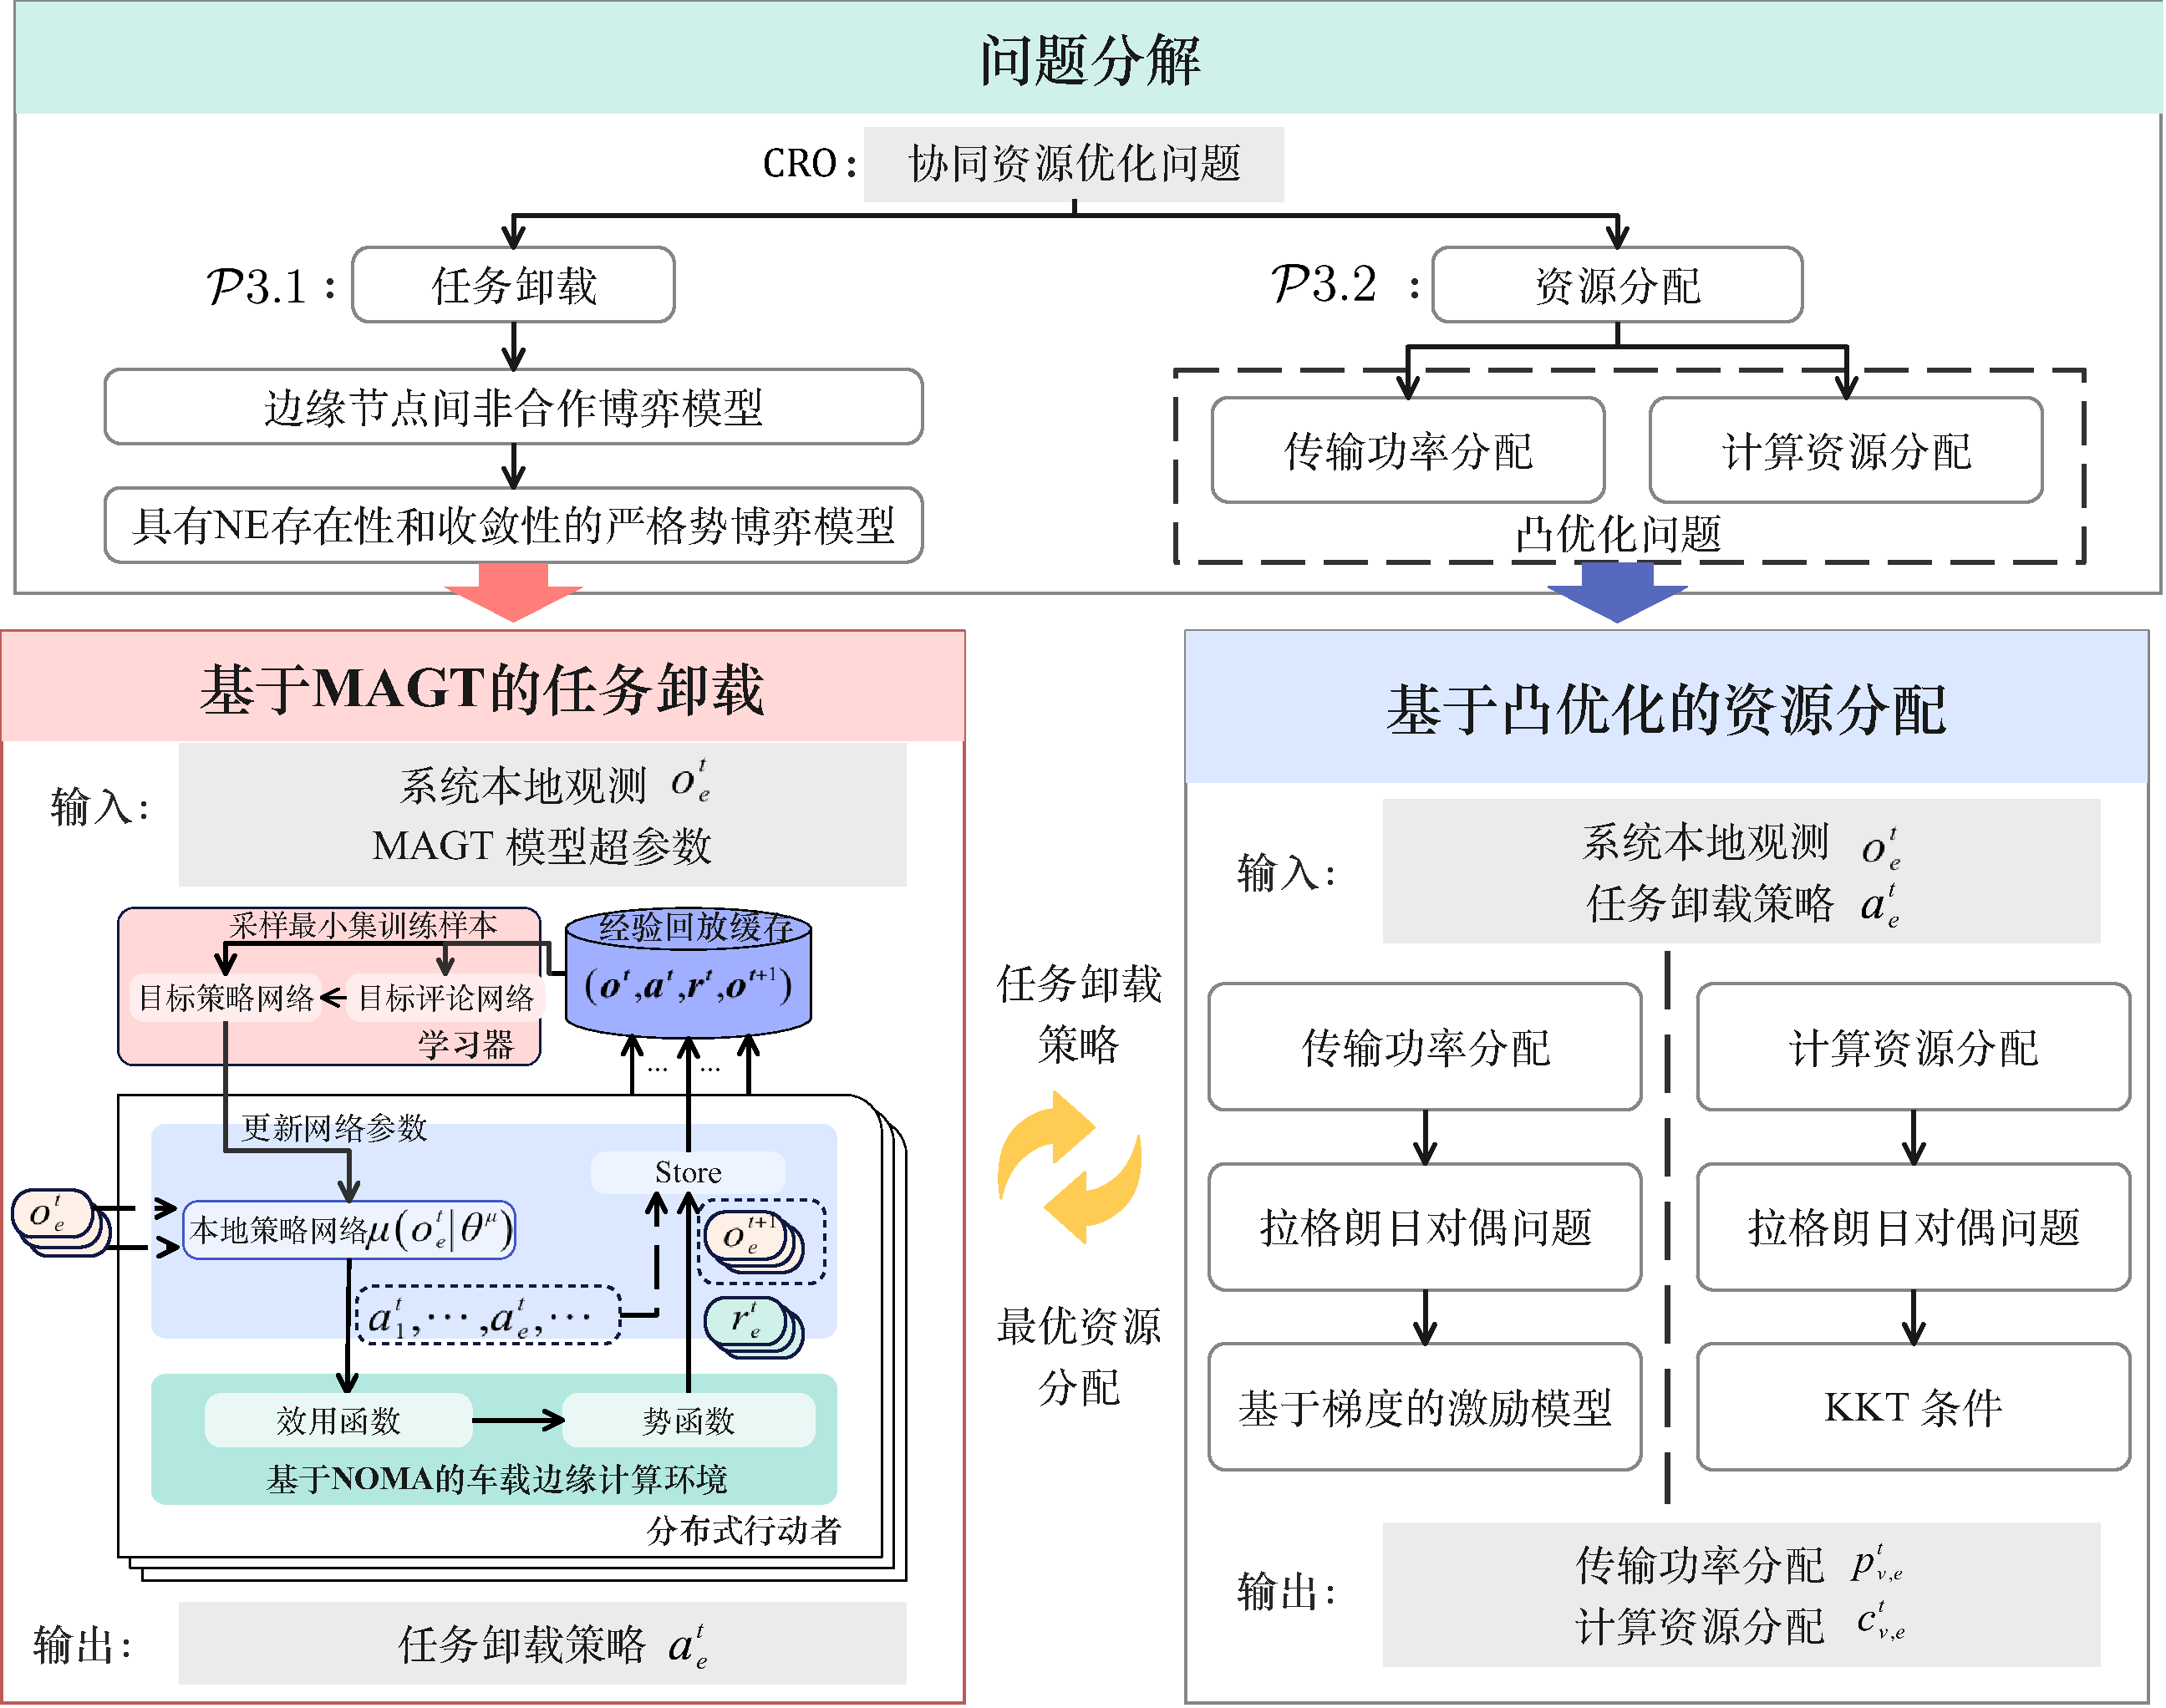
\includegraphics[width=1\columnwidth]{Fig4-3-solution-model.pdf}
  \bicaption{基于博弈理论的多智能体深度深度强化学习算法模型}{Multi-agent game-theoretic deep reinforcement learning model}
  \label{fig 3-3}
\end{figure} 

\subsection{问题分解}
在本节中,首先将CRO分解为单个时间片的多个问题。
由于$\mathbf{P}^{t}$、$\mathbf{Q}^{t}$和$\mathbf{C}^{t}$在时间$t$的变量是相互独立的,并且变量不重叠,四个约束条件是可分离的,所以CRO可以分解为两个子问题,其表述如下:

\textbf{1) 任务卸载:} 第一个任务卸载子问题$\mathcal{P}3.1$只涉及边缘节点的任务卸载决策$\mathbf{Q}^{t}$,其表述为
\begin{equation}
	\begin{aligned}
		\mathcal{P}3.1: &\max_{\mathbf{Q}^{t}} g_1= \sum_{ \forall e \in \mathbf{E}} \Psi_{e}^{t}  \\
		\text { s.t. }  
		&\mathcal{C}3.5: q_{v, e}^t \in \left \{0, 1\right \}, \forall v \in \mathbf{V}, \forall e \in \mathbf{E}  \\
        &\mathcal{C}3.6: \sum_{\forall e \in \mathbf{E}} q_{v, e}^t = 1, \forall v \in \mathbf{V} \\
	\end{aligned}
\end{equation}
然后,将 $\mathcal{P}3.1$ 建模为边缘节点之间的非合作博弈,其中边缘节点作为玩家,独立决定任务卸载策略。
该博弈模型表示为
\begin{equation}
	\mathcal{G} = \left\{\mathbf{E}, \mathbb{S}, \left\{{U}_{e}\right\}_{\forall e \in \mathbf{E}} \right\}
\end{equation}
其中$\mathbf{E}$表示玩家的集合;
$\mathbb{S}$ 表示博弈的策略空间,其被定义为所有边缘节点的单独策略集的笛卡尔乘积,即$\mathbb{S} = \mathbf{S}_{1} \times \ldots \times \mathbf{S}_{e} \times \ldots \times \mathbf{S}_{E}$,其中$\mathbf{S}_{e}$表示边缘节点$e$的所有可能策略集。
$\mathbb{S}$中的每个元素$\mathcal{S}$都是一个具体策略,$\mathcal{S} = \left(\mathcal{S}_{1}, \ldots, \mathcal{S}_{e}, \ldots, \mathcal{S}_{E} \right)$,并可以改写为 $\mathcal{S}=\left( \mathcal{S}_{e}, \mathcal{S}_{-e}\right)$,其中 $\mathcal{S}_{-e}$ 表示边缘节点 $e$ 的对手(即$\forall e^{\prime} \in \mathbf{E} \setminus \{e\}$)所采取的联合策略。
而$\mathcal{S}_{e}$是边缘节点$e$的策略,可以用$\mathcal{S}_{e} = \left\{ q_{v, e}^t \mid \forall e \in \mathbf{E}, \forall v \in \mathbf{V}_{e}^{t} \right\}$表示。
${U}_{e}\left(\mathcal{S}\right)$表示边缘节点$e$的效用函数,其定义如下:
\begin{definition}
边缘节点$e$的效用函数用${U}_{e}\left(\mathcal{S}\right): \mathbb{S} \mapsto \mathbb{R}$表示, 其被定义为策略概况下$\mathcal{S}$边缘节点的服务率之和,其中$\mathbb{R}$为实数集。
	\begin{equation}
		{U}_{e}\left(\mathcal{S}\right) = \sum_{\forall e \in \mathbf{E}} \Psi_{e}^{t}
	\end{equation}
\end{definition}

此外,本章通过给定一个势函数如公式\ref{equ 3-16}所示,证明该非合作博弈模型$\mathcal{G}$是一个具有NE存在和收敛性的EPG。
\begin{theorem}
给定边缘节点 $e$的势函数如下
\begin{equation}
	{F}_{e}\left(\mathcal{S}\right) = {U}_{e}\left(\mathcal{S}_{e}, \mathcal{S}_{-e}\right) - {U}_{e}\left(-\mathcal{S}_{e}, \mathcal{S}_{-e}\right)
	\label{equ 3-16}
\end{equation}
该博弈 $\mathcal{G}$ 是一个严格势博弈。
\label{theorem 4-1}
\end{theorem}
\noindent 其中${U}_{e}\left(-\mathcal{S}_{e}, \mathcal{S}_{-e}\right)$是边缘节点$e$的策略无效时的效用值。
\begin{proof} 见附录 \ref{appendix f}。
\end{proof}
\noindent 在博弈模型$\mathcal{G}$中,边缘节点试图在利益冲突的情况下通过最大化其效用来实现纳什均衡 \cite{chew2016potential}。
\begin{definition}
策略$\mathcal{S}^{*} \in \mathbb{S}$是一个纯策略的纳什均衡\cite{chew2016potential}当且仅当
	\begin{equation}
		U_{e}\left(\mathcal{S}_{e}^{*}, \mathcal{S}_{-e}^{*}\right) \geq U_{e}\left(\mathcal{S}_{e}, \mathcal{S}_{-e}^{*}\right), \quad \forall \mathcal{S}_{e} \in \mathbf{S}_{e}, \forall e \in \mathbf{E}
	\end{equation}
\end{definition}
\begin{lemma}
	给定一个势函数 $F_{e}(\mathcal{S})$ 如公式\ref{equ 3-16}所示,博弈 $\mathcal{G}$ 的NE 集合恰好和博弈$\mathcal{G}^{F}=\left\{\mathbf{E}, \mathbb{S}, \left\{{F}_{e}\right\}_{\forall e \in \mathbf{E}} \right\}$的NE集合一致,即
	\begin{equation}
		\mathcal{NE}(\mathcal{G}) \equiv \mathcal{NE}\left(\mathcal{G}^{F}\right)
	\end{equation}
	其中 $\mathcal{NE}$ 表示博弈模型的NE集合。
\label{lemma 4-1}
\end{lemma}
\begin{proof} 见附录 \ref{appendix g}。
\end{proof}
\noindent 最后, 本章基于引理\ref{lemma 4-1}证明博弈模型 $\mathcal{G}$ 具有纳什均衡的存在性。
\begin{theorem}
	给定势函数 $F_{e}(\mathcal{S})$ 如公式 \ref{equ 3-16},博弈 $\mathcal{G}$ 至少有一个纯策略的NE。
\label{theorem 4-2}
\end{theorem}
\begin{proof} 见附录 \ref{appendix h}。
\end{proof}
\noindent 另一方面,由于策略空间$\mathbb{S}$有限,NE可以在有限的步骤中收敛。
本章建立了$\epsilon$改进路径和$\epsilon$平衡点\cite{chew2016potential},其为一个近似于真实NE的策略,然后证明NE的收敛性。
\begin{definition} 
	路径 $\rho=\left(\mathcal{S}^{0}, \mathcal{S}^{1}, \mathcal{S}^{2}, \ldots\right)$ 是 $\epsilon$改进路径 \cite{chew2016potential},当其向前进任何一步 $i$,边缘节点 $e$ 的效能都提升了$\epsilon$,即 $U_{e}\left(\mathcal{S}^{i+1}\right) > U_{e}\left(\mathcal{S}^{i}\right) + \epsilon, \exists \epsilon \in \mathbb{R}_{+}, \forall i$。
\end{definition}
\begin{definition}
	策略 $\mathcal{\hat{S}} \in \mathbb{S}$ 是一个 $\epsilon$均衡 \cite{chew2016potential} 当且仅当 $\exists \epsilon \in \mathbb{R}_{+}$,并且
	\begin{equation}
		U_{e}\left(\mathcal{\hat{S}}_{e}, \mathcal{\hat{S}}_{-e}\right) \geq U_{e}\left(\mathcal{S}_{e}, \mathcal{\hat{S}}_{-e}\right) - \epsilon, \quad \forall \mathcal{S}_{e} \in \mathbf{S}_{e}, \forall e \in \mathbf{E}
	\end{equation}
\end{definition}
\begin{theorem}
对于博弈$\mathcal{G}$,每条$\epsilon$改进路径的步数都是有限的,其终点是$\epsilon$均衡,其是对原始NE的改进。
\label{theorem 4-3}
\end{theorem}
\begin{proof} 见附录 \ref{appendix i}。
\end{proof}

\textbf{2) 资源分配:} 第二个子问题$\mathcal{P}3.2$涉及传输功率分配$\mathbf{P}^{t}$和计算资源分配$\mathbf{C}^{t}$,其表述如下
\begin{align}
	\mathcal{P}3.2: &\min_{\mathbf{P}^{t}, \mathbf{C}^{t}} g_2= \sum_{ \forall e \in \mathbf{E}} \sum_{\forall k_{v}^{t} \in \mathbf{K}_{e}^{t}} \left( m_{v, e}^{t} +  n_{v, e}^{t} \right) \notag \\
	\text { s.t. }
    &\mathcal{C}3.7: \sum_{\forall v \in \mathbf{V}_{e}^{t}} p_{v, e}^{t} \leq p_{e}, \forall e \in \mathbf{E} \notag \\
    &\mathcal{C}3.8: \sum_{\forall k_{v}^{t} \in {\mathbf{K}_{q_e}^{t} }} c_{v, e}^t \leq c_{e}, \forall e \in \mathbf{E}
\label{equ 3-21}
\end{align}

\noindent 可以看出,公式\ref{equ 3-21}中的$\mathbf{P}^{t}$和$\mathbf{C}^{t}$的变量是相互独立的。
同时,因为变量没有重叠,限制条件$\mathcal{C}3.7$和$\mathcal{C}3.8$是可分离的。
因此,子问题$\mathcal{P}3.2$可以分为两个独立的问题,即传输功率分配和计算资源分配,其表述如下:

\textbf{传输功率分配:} 其只涉传输功率分配变量$\mathbf{P}^{t}$,其表述如下
\begin{align}
	\mathcal{P}3.3: &\min_{\mathbf{P}^{t}} g_3= \sum_{ \forall e \in \mathbf{E}} \sum_{\forall k_{v}^{t} \in \mathbf{K}_{e}^{t}}  \frac{d_{k}}{b  \log _{2}\left(1+\mathrm{SINR}_{v, e}^t\right)} \notag \\
	&\text { s.t. } \mathcal{C}3.7: \sum_{\forall v \in \mathbf{V}_{e}^{t}} p_{v, e}^{t} \leq p_{e}, \forall e \in \mathbf{E}
\end{align}
显然,与边缘节点相关的变量是独立的。
因此,$\mathcal{P}3.3$可以进一步划分为多个简单问题,其中每个问题只与单个边缘节点$e$有关。
\begin{align}
	\mathcal{P}3.4: & \max_{\mathbf{P}_{e}^{t}}  g_3^e= \sum_{\forall k_{v}^{t} \in \mathbf{K}_{e}^{t}} {b  \log _{2}\left(1+\mathrm{SINR}_{v, e}^t\right)} \notag \\
	&\text { s.t. } \mathcal{C}3.9: \sum_{\forall v \in \mathbf{V}_{e}^{t}} p_{v, e}^{t} \leq p_{e}  
\end{align}
然而,由于边缘内和边缘间的干扰,$\mathcal{P}3.4$是非凸的。
然后,本章应用近似方法将$\mathcal{P}3.4$转换成一个凸问题。
特别地,$g_3^e$的下界可以通过下式得到\cite{papandriopoulos2006low}。
\begin{equation}
	g_3^e \geq \overline{g_3^e} = \sum_{\forall k_{v}^{t} \in \mathbf{K}_{e}^{t}} {b \left( \xi_{v, e}^{t} \log _{2}\mathrm{SINR}_{v, e}^t + \omega_{v, e}^{t} \right) }
\end{equation}
其中,$\xi_{v, e}^{t}$ 和 $\omega_{v, e}^{t}$ 是固定值并由下式给出。
\begin{align}
	\xi_{v, e}^{t} &= \overline{\mathrm{SINR}}_{v, e}^t \bigg/ ( 1 + \overline{\mathrm{SINR}}_{v, e}^t ) \\
	\omega_{v, e}^{t} &= \log _{2} (1+ \overline{\mathrm{SINR}}_{v, e}^t) - \frac{\overline{\mathrm{SINR}}_{v, e}^t}{1 + \overline{\mathrm{SINR}}_{v, e}^t} \log _{2}\overline{\mathrm{SINR}}_{v, e}^t
\end{align}
如果${\mathrm{SINR}}_{v, e}^t =\overline{\mathrm{SINR}}_{v, e}^t$,该下界是紧的。
因此,$\mathcal{P}3.4$可以松弛后重新表达为
\begin{align}
	\mathcal{P}3.5: & \max_{\mathbf{P}_{e}^{t}}  \overline{g_3^e}= \sum_{\forall k_{v}^{t} \in \mathbf{K}_{e}^{t}} {b \left( \xi_{v, e}^{t} \log _{2}\mathrm{SINR}_{v, e}^t + \omega_{v, e}^{t} \right) } \notag \\
	&\text { s.t. } \mathcal{C}3.9: \sum_{\forall v \in \mathbf{V}_{e}^{t}} p_{v, e}^{t} \leq p_{e}  
\end{align}
尽管如此,$\mathcal{P}3.5$仍然是非凸的,因为目标在$\mathbf{P}_{e}^{t}$中不是凹的。
给定一个新的变量$\widetilde{p_{v, e}^t} = \log _{2} {p}_{v, e}^t$,$\mathcal{P}3.5$可以被转化为如下形式
\begin{align}
	\mathcal{P}3.6: & \max_{\widetilde{\mathbf{{P}}_{e}^{t}}}  \widetilde{g_3^{e}}= \sum_{\forall k_{v}^{t} \in \mathbf{K}_{e}^{t}} {b ( \xi_{v, e}^{t} \log _{2}\mathrm{\widetilde{SINR}}_{v, e}^t + \omega_{v, e}^{t} ) } \notag \\
	&\text { s.t. } \mathcal{C}3.10: \sum_{\forall v \in \mathbf{V}_{e}^{t}} 2^{\widetilde{p_{v, e}^t}} \leq p_{e}  
\end{align}
其中 $\log _{2}\mathrm{\widetilde{SINR}}_{v, e}^t$ 由以下公式给出
\begin{align}
	\log _{2}\mathrm{\widetilde{SINR}}_{v, e}^t &= \widetilde{p_{v, e}^t} + \log _{2} |h_{v, e}^t| ^{2} - \log _{2} \left( \sum\limits_{\forall v^{\prime} \in \mathbf{V}_{h_{v, e}}^{t}} |h_{v^{\prime}, e}^t|^2 2^{\widetilde{p_{v^{\prime}, e}^{t}}} \right. \notag \\
	&+ \left. \sum\limits_{\forall e^{\prime} \in \mathbf{E} / \{e\}} \sum\limits_{\forall v^{\prime} \in \mathbf{V}_{e^{\prime}}^{t}} |h_{v^{\prime}, e}^t|^2 2^{\widetilde{p_{v^{\prime}, e^{\prime}}^{t}}} + N_{0}\right)
\end{align}
\noindent 因此,$\mathcal{P}3.6$是一个标准的凹最大化问题,也是一个凸优化问题,因为每个约束条件都是凸型指数之和,而目标之和中的每项都是凹的。

\textbf{计算资源分配:} 其是关于$\mathbf{C}^{t}$变量的计算资源分配,其表述如下
\begin{align}
	\mathcal{P}3.7: &\min_{\mathbf{C}^{t}} g_4= \sum_{ \forall e \in \mathbf{E}} \sum_{\forall k_{v}^{t} \in \mathbf{K}_{e}^{t}} ( w_{v, e}^{t} + \sum_{\forall e^{\prime} \in \mathbf{E}} q_{v, e^{\prime}}^{t} x_{v, e^{\prime}}^t) \notag \\
	&\text { s.t. } \mathcal{C}3.8:  \sum_{\forall k_{v}^{t} \in {\mathbf{K}_{q_e}^{t} }} c_{v, e}^t \leq c_{e}, \forall e \in \mathbf{E}
\end{align}
与公式中的$\mathcal{P}3.3$类似,$\mathcal{P}3.7$可以进一步分解为多个简单问题,每个问题只与一个边缘节点$e$有关,其表述如下
\begin{align}
	\mathcal{P}3.8: &\min_{\mathbf{C}_{e}^{t}} g_4^e= \sum_{\forall a_{v}^{t} \in {\mathbf{K}_{q_e}^{t} }}   x_{v, e}^t \notag \\
	&\text { s.t. } \mathcal{C}3.11:  \sum_{\forall k_{v}^{t} \in {\mathbf{K}_{q_e}^{t} }} {c_{v, e}^t} \leq c_{e}
\label{equ 3-29}
\end{align}
\noindent 其中${\mathbf{C}_e^t}$代表${\mathbf{C}^{t}}$中与边缘节点$e$相关的变量。
因此,$\mathcal{P}3.8$是一个凸优化问题,因为公式\ref{equ 3-29} 中的目标是凸的,而约束是线性的。

\subsection{基于MAGT的任务卸载}
MAGT模型由若干个分布式行动者、一个学习器、一个基于NOMA的VEC环境和一个经验回放缓存组成。
MAGT的主要组成部分设计如下:

\textbf{1) 系统状态:} 边缘节点$e$在时间$t$上对系统状态的局部观察被表示为
	\begin{equation}
		\boldsymbol{o}_{e}^{t}=\left\{e, t, \mathbf{Dis}_{\mathbf{V}_{e}^{t}}, \mathbf{D}_{\mathbf{K}_{e}^{t}}, \mathbf{C}_{\mathbf{K}_{e}^{t}}, \mathbf{T}_{\mathbf{K}_{v}^{t}}\right\}
	\end{equation} 
	\noindent 其中$e$是边缘节点索引;
	$t$是时隙索引;
	$\mathbf{Dis}_{\mathbf{V}_{e}^{t}}$代表$e$在时间$t$的边缘节点和车辆$v \in \mathbf{V}_{e}^{t}$之间的距离集合;
	$\mathbf{D}_{\mathbf{K}_{e}^{t}}$、$\mathbf{C}_{\mathbf{K}_{e}^{t}}$和$\mathbf{T}_{\mathbf{K}_{v}^{t}}$分别代表$t$时边缘节点$e$中的$k_{v}^{t} \in \mathbf{K}_{e}^{t}$的数据大小、所需计算资源和截止时间。
	因此,时间$t$的系统状态可表示为$\boldsymbol{o}^{t}=\left\{\boldsymbol{o}_{1}^{t}, \ldots, \boldsymbol{o}_{e}^{t}, \ldots, \boldsymbol{o}_{E}^{t}\right\}$。

\textbf{2) 动作空间:} 边缘节点$e$的动作空间由车辆$v \in \mathbf{V}_{e}^{t}$请求任务的卸载决策组成,其表示为
	\begin{equation}
		\boldsymbol{a}_{e}^{t} = \left\{ q_{v, e^{\prime}}^t \mid \forall e^{\prime} \in \mathbf{E}, \forall v \in \mathbf{V}_{e}^{t} \right\}
	\end{equation}
	\noindent 其中,$q_{v, e^{\prime}}^t \in \{0, 1\}$表示任务$k_{v}^t$是否在边缘节点$e^{\prime}$中被卸载。
	边缘节点动作的集合表示为 $\boldsymbol{a}^{t} = \left\{\boldsymbol{a}_{e}^{t}\mid \forall e \in \mathbf{E} \right\}$.
	
\textbf{3) 奖励函数:} 在博弈模型中,每个边缘节点的目标是使其效用最大化。
	因此,系统的奖励函数被定义为边缘节点在时间$t$实现的效用,其表示方法为
	\begin{equation}
		r\left(\boldsymbol{a}^{t} \mid \boldsymbol{o}^{t}\right)= {U}_{e}\left(\mathcal{S}_{e}, \mathcal{S}_{-e}\right) = \sum_{\forall e \in \mathbf{E}} \Psi_{e}^{t}
		\label{equ 3-32}
	\end{equation}
	此外,博弈$\mathcal{G}$ 的势函数被采纳为边缘节点在系统状态$\boldsymbol{o}^{t}$下的行动$\boldsymbol{a}_{e}^{t}$的奖励。
	\begin{equation}
		r_{e}^{t} = r\left(\boldsymbol{a}^{t} \mid \boldsymbol{o}^{t}\right)-r\left(\boldsymbol{a}_{-e}^{t} \mid \boldsymbol{o}^{t}\right)
		\label{equ 3-33}
	\end{equation}
	\noindent 其中$r\left(\boldsymbol{a}_{-e}^{t} \mid \boldsymbol{o}^{t}\right)$是在没有边缘节点$e$贡献的情况下实现的系统奖励,它可以通过设置边缘节点$e$的空动作集得到。
	边缘节点的奖励集合用$\boldsymbol{r}^{t} = \{r_{1}^{t}, \ldots, r_{e}^{t}, \ldots, r_{E}^{t}\}$。
	在MAGT中,每个边缘节点 $e \in \mathbf{E}$的目标是最大化预期收益,用$R_{e}^{t} = \sum_{i \geq 0} \gamma^{i} r_{e}^{t+i}$表示,其中$\gamma$是折扣系数。

在MAGT的开始阶段,本地策略和评论家网络的参数在学习器中被随机初始化,其分别用 $\theta^{\mu}$和$\theta^{Q}$表示。
然后,目标策略和评论家网络的参数被初始化为与相应的本地网络相同,分别用$\theta^{\mu^{\prime}}$和$\theta^{Q^{\prime}}$表示。
\begin{align}
	\theta^{\mu^{\prime}} \leftarrow \theta^{\mu}\\
	\theta^{Q^{\prime}} \leftarrow \theta^{Q}
\end{align}
而经验回放缓存$\mathcal{B}$被初始化为最大存储大小$|\mathcal{B}|$,以存储回放经验。

\SetKwInOut{KwIn}{输入}
\SetKwInOut{KwOut}{输出}

\begin{algorithm}[h]\small
\renewcommand{\algorithmcfname}{算法}
	\caption{基于博弈理论的多智能深度强化学习}
\KwIn{折扣因子 $\gamma$、批大小 $M$、样本长度 $N$、回放经验缓存 $\mathcal{B}$、探索常数 $\epsilon$、学习率$\alpha$和$\beta$、目标网络参数更新周期 $t_{\operatorname{tgt}}$、分布式行动者网络参数更新周期 $t_{\operatorname{act}}$}
\KwOut{任务卸载决策$q_{v, e^{\prime}}^t$、传输功率分配策略$p_{v, e}^{t, {(i+1)}}$、计算资源分配策略${c_{v, e}^{t}}^{\star}$}
	初始化网络参数\\
	初始化经验回放缓存 $\mathcal{B}$\\
	\For{\songti{分布式行动体} $j = 1$ \songti{到} $J$}{
			初始化一个随机过程 $\mathcal{N}$ 以进行探索\\
			行动体从学习器中复制网络参数\\
			接收初始系统状态 $\boldsymbol{o}_{1}$\\
			\For{\songti{时间片} $t = 1$ \songti{到} $T$}{
				\For{\songti{边缘节点} $e=1$ \songti{到} $E$}{
					接收本地观测 $\boldsymbol{o}_{e}^{t}$\\
					选择一个动作 $\boldsymbol{a}_{e}^{t}=\boldsymbol{\mu}\left(\boldsymbol{o}_{e}^{t} \mid \theta^{\mu}_{j}\right)+\mathcal{N}_{t}$\\
					基于梯度的迭代方法得到最优传输功率分配\\
					基于KKT条件得到最优计算资源分配\\
				}
				接收奖励 $\boldsymbol{r}^{t}$ 和下一个系统状态 $\boldsymbol{o}^{t+1}$\\
				存储 $\left(\boldsymbol{o}^{t}, \boldsymbol{a}^{t}, \boldsymbol{r}^{t}, \boldsymbol{o}^{t+1}\right)$ 到经验回放缓存 $\mathcal{B}$;
			}
	}
	\For{\songti{迭代次数} $= 1$ \songti{到最大迭代次数}}{
		\For{\songti{时间片} $t = 1$ \songti{到} $T$}{
			\For{\songti{边缘节点} $e=1$ \songti{到} $E$}{
				从经验回放缓存$\mathcal{B}$随机采样长度为$N$ 的$M$ 最小样本集\\
				构建目标分布\\
				计算策略和评论家网络损失\\
				更新本地策略和评论家网络
			}
			\If{$t \mod t_{\operatorname{tgt}} = 0$}{
				更新目标网络\\
			}
			\If{$t \mod t_{\operatorname{act}} = 0$}{
				复制网络参数给分布式行动者
			}
		}
	}
\label{algorithm 3-1}
\end{algorithm}

另一方面,$J$个分布式行动者通过与环境同时交互而产生重放经验。
第$j$个角色的本地策略网络的参数是从学习器的本地策略网络中复制得到的,用$\theta^{\mu}_{j}$表示。
每次迭代的初始化系统状态用$\boldsymbol{o}^{0}$表示。
根据对系统状态的局部观察,得到第$j$个行为体中的边缘节点$e$在时间$t$的任务卸载动作。
\begin{equation}
	\boldsymbol{a}_{e}^{t}={\mu}\left(\boldsymbol{o}_{e}^{t} \mid \theta^{\mu}_{j}\right)+\epsilon  \mathcal{N}_{t}
\end{equation}
\noindent 其中,$\mathcal{N}_{t}$为探索噪声,以增加边缘行动的多样性,$\epsilon$为探索常数。
然后,边缘节点的动作$\boldsymbol{a}^{t}$在基于NOMA的VEC环境中执行,每个边缘节点的奖励可以根据公式\ref{equ 3-33}得到。
最后,包括当前系统状态$\boldsymbol{o}^{t}$、边缘节点动作$\boldsymbol{a}^{t}$、边缘节点奖励$\boldsymbol{r}^{t}$和下一时刻系统状态$\boldsymbol{o}^{t+1}$在内的交互经验被存储到经验回放缓存$\mathcal{B}$。
迭代将继续进行,直到学习器完成训练过程。

从经验回放缓存$\mathcal{B}$中抽取长度为$N$的$M$样本的小批量,以训练学习器的策略和评论家网络。
$M$小批量中样本用$\left(\boldsymbol{o}^{i:i+N}, \boldsymbol{a}^{i:i+N-1}, \boldsymbol{r}^{i:i+N-1}\right)$来表示。
边缘节点$e$的目标分布用$Y_e^i$表示,其计算方法为:
\begin{equation}
	Y_e^{i} = \sum_{n=0}^{N-1} \left( \gamma^{n} r_{e}^{i+n}\right)+\gamma^{N} Q^{\prime}\left(\boldsymbol{o}_{e}^{i+N}, \boldsymbol{a}^{i+N} \mid \theta^{Q^{\prime}} \right)
\end{equation}
\noindent 其中 $\boldsymbol{a}^{i+N} = \{ \boldsymbol{a}_{1}^{i+N}, \ldots, \boldsymbol{a}_{e}^{i+N}, \ldots, \boldsymbol{a}_{E}^{i+N} \}$ 且 $\boldsymbol{a}_{e}^{i+N}$ 是通过目标策略网络得到的, 即$\boldsymbol{a}_{e}^{i+N} = \mu^{\prime}(\boldsymbol{o}_{e}^{i+N} \mid \theta^{\mu^{\prime}})$。
评论家网络的损失函数表示为
\begin{equation}
	{L}\left(\theta^{Q}\right)=\frac{1}{M} \sum_{i} \frac{1}{E} \sum_{e} \left(Y_e^{i}-Q\left(\boldsymbol{o}_{e}^{i}, \boldsymbol{a}^{i} \mid \theta^{Q}\right)\right)^{2}
\end{equation}
策略网络的参数通过策略梯度进行更新。
\begin{equation}
	\nabla_{\theta^{\mu}} \mathcal{J} = \frac{1}{M} \sum_{i} \frac{1}{E} \sum_{e} \nabla_{\boldsymbol{a}_{e}^{i}} Q\left(\boldsymbol{o}_{e}^{i}, \boldsymbol{a}^{i} \mid \theta^{Q}\right) \nabla_{\theta^{\mu}} \mu\left(\boldsymbol{o}_{e}^{i} \mid \theta^{\mu}\right)
\end{equation}
本地策略网络和本地评论家网络的参数以学习率$\alpha$和$\beta$更新。
最后,如果$t\mod t_{\operatorname{tgt}}=0$,边缘节点更新目标网络的参数,其中$t_{\operatorname{tgt}}$为目标网络参数更新周期。
\begin{align}
	\theta^{\mu^{\prime}} &\leftarrow n \theta^{\mu}+(1-n)  \theta^{\mu^{\prime}}\\
	\theta^{Q^{\prime}} &\leftarrow n  \theta^{Q}+(1-n) \theta^{Q^{\prime}}
\end{align}
\noindent 其中 $n \ll 1$。
第$j$个行为者的策略网络参数也会定期更新,即当$t \mod t_{\operatorname{act}} = 0$时,其中$t_{\operatorname{act}}$是分布式行为者的网络参数更新周期。
\begin{equation}
	\theta_{j}^{\mu} \leftarrow \theta^{\mu^{\prime}}, \forall j
\end{equation}
其中$\theta_{j}^{\mu}$表示第$j$个分布式行为体中的本地策略网络参数。
	
\subsection{基于凸优化的资源分配}
\textbf{1) 传输功率分配:} 为了解决凸优化问题$\mathcal{P}3.6$,本章首先利用拉格朗日对偶法\cite{boyd2004convex},在$\mathcal{P}3.6$中引入拉格朗日乘数$\lambda_{e}^{t}$,拉格朗日函数如下:
\begin{equation}
	\mathcal{L}(\widetilde{\mathbf{{P}}_{e}^{t}}, {\lambda}_{e}^{t} ) = \widetilde{g_3^{e}} -  {\lambda}_{e}^{t} (\sum_{\forall v \in \mathbf{V}_{e}^{t}} 2^{\widetilde{p_{v, e}^{t}}} - p_{e} )
	\label{equ 3-41}
\end{equation}
此外,$\mathcal{P}3.6$的对偶问题可表示为
\begin{align}
	\mathcal{P}3.9: & \min_{{\lambda}_{e}^{t}} \max_{\widetilde{\mathbf{{P}}_{e}^{t}}}  g_5 = \mathcal{L}(\widetilde{\mathbf{{P}}_{e}^{t}}, {\lambda}_{e}^{t} ) \notag \\
	&\text { s.t. } \mathcal{C}3.12: \mathbf{\lambda}_{e}^{t} \geq 0  
\end{align}
因此,$\mathcal{P}3.9$可以分解为两层优化问题。
内层表示为固定${\lambda}_{e}^{t}$的$\widetilde{\mathbf{{P}}_{e}^{t}}$的优化问题,外层表示为固定$\widetilde{\mathbf{{P}}_{e}^{t}}$的${\lambda}_{e}^{t}$优化问题。
在外层,对偶变量${\lambda}_{e}^{t}$通过梯度下降迭代更新。
\begin{equation}
	\mathbf{\lambda}_{e}^{t, (i+1)} = \max\left\{0, \mathbf{\lambda}_{e}^{t, (i)} + \sigma (\sum_{\forall v \in \mathbf{V}_{e}^{t}} 2^{\widetilde{p_{v, e}^{t}}} - p_{e} )\right\}
\end{equation}
其中$\widetilde{p_{v, e}^{t}}$是固定的;$\sigma$是一个足够小的常数,$i$是一个迭代次数。
此外,内部对偶最大化可以通过寻找公式\ref{equ 3-41}中拉格朗日函数静止点来解决,即相对于$\widetilde{\mathbf{{P}}_{e}^{t}}$固定${\lambda}_{e}^{t}$。
\begin{equation}
\frac{\partial \mathcal{L}\left(\widetilde{\mathbf{{P}}_{e}^{t}}, \mathbf{\lambda}_{e}^{t} \right)}{\partial \widetilde{p_{v, e}^{t}}}= b  \xi_{v, e}^{t}  - p_{v, e}^{t}(\lambda_{e}^{t} +\sum\limits_{\forall v^{\prime} \in \mathbf{V}_{h_{v, e}}^{t}} b  \xi_{v, e}^{t} |h_{v, e}^t|^2 \frac{\mathrm{SINR}_{v^{\prime}, e}^t}{|h_{v^{\prime}, e}^t| ^{2} p_{v^{\prime}, e}^{t}}) =0
\end{equation}
其中,偏导数被转换回$\mathbf{P}_{e}^{t}$空间。
因此,可以列出定点方程,车辆$v$的传输功率通过以下方式更新。
\begin{equation}
p_{v, e}^{t, {(i+1)}}=\frac{b \xi_{v, e}^{t}}{\lambda_{e}^{t,(i)}+\sum\limits_{\forall v^{\prime} \in \mathbf{V}_{h_{v, e}}^{t}} b  \xi_{v, e}^{t}|h_{v, e}^t|^2 {I}_{v^{\prime}, e}^{t, (i)} }
\end{equation}
其中$\lambda_{e}^{t,(i)}$和$p_{v, e}^{t, (i+1)}$分别表示$\lambda_{e}^{t}$和$p_{v, e}^{t}$在$i$次迭代的值,${I}_{v^{\prime}, e}^{t, (i)}$由如下公式给出。
\begin{equation}
	{I}_{v^{\prime}, e}^{t, (i)} = \sum\limits_{\forall v^{\prime} \in \mathbf{V}_{h_{v, e}}^{t}} |h_{v^{\prime}, e}^t|^2 p_{v^{\prime}, e}^{t, (i)} + \sum\limits_{\forall e^{\prime} \in \mathbf{E} / \{e\}} \sum\limits_{\forall v^{\prime} \in \mathbf{V}_{e^{\prime}}^{t}} |h_{v^{\prime}, e}^t|^2 p_{v^{\prime}, e^{\prime}}^{t, (i)} + N_{0}
\end{equation}
其中 $p_{v^{\prime}, e}^{t, (i)}$ 和 $p_{v^{\prime}, e^{\prime}}^{t, (i)}$ 分别表示 $p_{v^{\prime}, e}^{t}$ 和 $p_{v^{\prime}, e^{\prime}}^{t}$ 在 $i$次迭代的值。

\textbf{2) 计算资源分配:} 与传输功率分配类似,本章首先在$\mathcal{P}3.8$中引入拉格朗日乘数${\lambda}_{e}^{t}$。
然后,$\mathcal{P}3.8$的对偶问题可以表示为
\begin{align}
	\mathcal{P}3.10: & \min_{\mathbf{\lambda}_{e}^{t}, \mathbf{{C}}_{e}^{t}}  g_6 = g_4^e - {\lambda}_{e}^{t} (\sum_{\forall k_{v}^{t} \in {\mathbf{K}_{q_e}^{t} }} {c_{v, e}^t} - c_{e} ) \notag \\
		&\text { s.t. } \mathcal{C}3.12: \mathbf{\lambda}_{e}^{t} \geq 0 
\end{align}
基于KKT条件\cite{boyd2004convex},可以得到以下公式。
\begin{align}
	\nabla_{\mathbf{C}_e^{t}} g_4^e + \mathbf{\lambda}_{e}^{t}\nabla_{\mathbf{C}_e^{t}} (\sum_{\forall k_{v}^{t} \in {\mathbf{K}_{q_e}^{t} }} {c_{v, e}^t} - c_{e} ) &= 0, \notag \\
	\mathbf{\lambda}_{e}^{t}( \sum_{\forall k_{v}^{t} \in {\mathbf{K}_{q_e}^{t} }} {c_{v, e}^t} - {c_{e}} ) &= 0, \notag \\
	\mathbf{\lambda}_{e}^{t} &\geq 0
\end{align}
通过求解方程组,可以得到任务$k_{v}^{t}$的计算资源分配的最优方案如下:
\begin{equation}
	{c_{v, e}^{t}}^{\star} = \frac{1 / c_e \sqrt{d_k  c_k} } {\sum_{\forall k_{v}^{t} \in {\mathbf{K}_{q_e}^{t} }} 1 / c_e \sqrt{d_k  c_k}} , \forall k_{v}^{t} \in {\mathbf{K}_{q_e}^{t} } 
\end{equation}

\section{实验结果与分析}\label{section 3-5}

\subsection{实验设置}

在本章节中,本章通过使用Python 3.9.13和TensorFlow 2.8.0实现了一个仿真模型,以评估所提出的解决方案的性能。
仿真模型基于Ubuntu 20.04服务器,其配备AMD Ryzen 9 5950X 16核处理器(时钟频率为3.4 GHz),两个NVIDIA GeForce RTX 3090图形处理单元,以及64 GB内存。
本章考虑在一个3平方千米的正方形区边缘内的一般情况,其中$E=9$边缘节点,如5G基站和RSU均匀分布在场景图上。
在参考 \inlinecite{zhu2021decentralized}、 \inlinecite{liu2021rtds}、 \inlinecite{xu2021socially}和\inlinecite{zhou2019computation}的基础上,仿真实验参数设置如下:
边缘节点的计算能力(即CPU时钟频率)被设定为均匀分布在$[3, 10]$ GHz \cite{zhou2019computation}。 
V2I通信的通信范围被设定为$u_e =$ 500 m\cite{zhu2021decentralized}。
此外,利用现实的车辆轨迹作为交通输入,从滴滴GAIA开放数据集中提取2016年11月16日中国成都市青羊区3平方千米区域的数据。
特别地,本章研究了四个不同时期(即8:00-8:05、13:00-13:05、18:00-18:05,以及23:00-23:05)的服务场景。

为了实现MAGT,策略和评论家网络结构描述如下:
本地策略网络是一个有三个隐藏层的五层全连接神经网络,其中神经元的数量分别为256、256和256。
目标策略网络的结构与本地策略网络相同。
本地评论家网络是一个五层全连接神经网络,有三个隐藏层,其中神经元的数量分别是512、512和256。
目标批评家网络的结构与本地批评家网络相同。
利用ReLU作为激活函数,并使用Adam优化器来更新网络权重。
分布式行动者的数量设定为$J$=10。
主要的系统模型参数和算法参数显示在表\ref{table 3-1}和\ref{table 3-2}中。

\begin{table}[h]\small
\centering
\bicaption{系统模型参数}{Parameters of system model}
\setlength{\tabcolsep}{15mm}{
\begin{tabular}[t]{ccc}
\toprule
参数&值\\
\midrule
请求任务大小 $d_k$ \cite{liu2021rtds}&[0.01, 5] MB\\
处理1 bit 任务数据所需的计算资源 $c_k$ \cite{zhu2021decentralized} & 500 cycles/bit\\
任务的截止时间 $t_k$  \cite{liu2021rtds}&[5, 10] s\\
V2I 带宽 $b$ \cite{zhou2019computation}&20 MHz\\
边缘节点的计算能力 $c_e$ \cite{zhou2019computation}&[3, 10] GHz\\
V2I 通信最大传输功率 $p_e$ \cite{zhu2021decentralized}&1$\times 10^3$ mW\\
V2I 通信范围 $u_e$ \cite{zhu2021decentralized}&500 m\\
有线传输速率 $z$&50 Mbps\\
距离折扣 $\zeta$& 6.667$\times 10^{-4}$\\
加性白高斯噪声 $N_0$ \cite{xu2021socially}&-90 dBm\\
大尺度路径损耗指数 $\varphi$ \cite{xu2021socially}&3\\
\bottomrule
\end{tabular}}
\label{table 3-1}
\end{table}

\begin{table}[h]\small
\centering
\bicaption{MAGT模型参数}{Parameters of MAGT}
\setlength{\tabcolsep}{18.5mm}{
\begin{tabular}[t]{ccc}
\toprule
参数&值\\
\midrule
折扣因子 $\gamma$&0.996\\
批大小 $M$&256\\
回放缓存最大容量 $|\mathcal{B}|$&1$\times10^{6}$\\
探索常数 $\epsilon$&0.3\\
策略网络和评价家网络的学习率&1$\times10^{-4}$\\
目标网络参数更新周期 $t_{\operatorname{tgt}}$&100\\
分布式行动者网络参数更新周期 $t_{\operatorname{act}}$&1000\\
\bottomrule
\end{tabular}}
\label{table 3-2}
\end{table}
 
为了进行性能比较,本章实现了以下四种可比的算法。
\begin{itemize}
	\item \textbf{最优资源分配和任务全迁移}: 其分为两个阶段:资源分配和任务卸载。其中资源分配问题通过凸优化得到最优解,同时边缘节点倾向于将所有任务迁移到其他边缘节点。
	\item \textbf{最优资源分配和任务仅本地处理}: 其中资源分配与ORM算法相同,同时每个边缘节点倾向于在本地执行所有任务。
	\item \textbf{分布式深度确定性策略梯度} \cite{barth2018distributed}: 其通过实现一个以全局系统状态为输入的DDPG智能体,共同决定任务卸载决策、V2I传输功率分配和计算资源分配,其中效用函数被作为智能体的奖励。
	\item \textbf{多智能体深度确定性策略梯度}\cite{zhang2021adaptive}: 其中资源分配与ORM算法相同,并在每个边缘节点中实现MADDPG,以独立确定任务卸载决策,其中效用函数被作为边缘节点的奖励。
\end{itemize}

为了进行性能评估,本章收集以下统计数据。每个任务的上传时间和处理时间;本地执行的任务总数,用$K_{\operatorname{local}}$表示;迁移到其他边缘节点的任务数,用$K_{\operatorname{migrated}}$表示;任务总数,用$K_{\operatorname{total}}$表示,以及服务的任务数,用$K_{\operatorname{serviced}}$表示。
在此基础上,根据公式\ref{equ 3-9}、\ref{equ 3-10}、\ref{equ 3-11}和 \ref{equ 3-32}得到四个指标,即\textbf{平均处理时间}、\textbf{平均服务时间}、\textbf{平均服务率}(Average Service Ratio, ASR)和\textbf{累积奖励}。
本章进一步设计了以下两个额外的度量来进行分析。
\begin{itemize}
	\item \textbf{平均实现势} : 它被定义为边缘奖励的总和(即实现的势)除以调度期间的边缘节点数,其计算公式为
		\begin{equation}
		 	 \operatorname{AAP} = \frac{1}{E}\sum_{\forall e \in \mathbf{E}} \sum_{\forall t \in \mathbf{T}} r_{e}^{t}
		\end{equation}
	\item \textbf{本地处理与迁移的比例} : 本地处理的任务的比例可通过下式计算
		\begin{equation}
			P_{\operatorname{local}} = \frac{K_{\operatorname{local}}}{K_{\operatorname{total}}}
		\end{equation}
		而迁移到其他边缘节点的任务的比例计算如下 
		\begin{equation}
			P_{\operatorname{migrated}} = \frac{K_{\operatorname{migrated}}}{K_{\operatorname{total}}}
		\end{equation}
		且 $P_{\operatorname{local}} +P_{\operatorname{migrated}} = 1$。
\end{itemize}

\subsection{实验结果与分析}

\textbf{1) 算法收敛性:} 图\ref{fig 3-4}比较了五种算法在不同交通场景下的收敛性能以及CR。如图所示,MAGT的收敛速度仅次于D4PG(即3000次左右的迭代),但它却取得了最高的CR值(即230左右)。相比之下,D4PG和MADDPG分别经过2000和3500次左右的迭代后收敛,并实现了190和220左右的CR。而ORL和ORM分别实现了约210和189的CR。据观察,ORM、ORL、MADDPG和MAGT在前2000次迭代中可以达到比D4PG高得多的CR。主要原因是在ORM、ORL、MADDPG和MAGT中使用了提出的最优资源分配方案,使其性能优于共同决定任务卸载和资源分配的D4PG。另一方面,由于在MAGT中利用分布式行为者加速重放经验采样,所提出的解决方案比MADDPG收敛得更快,同时在不同的交通场景下实现了最高CR。

\begin{figure}[h]
\centering
  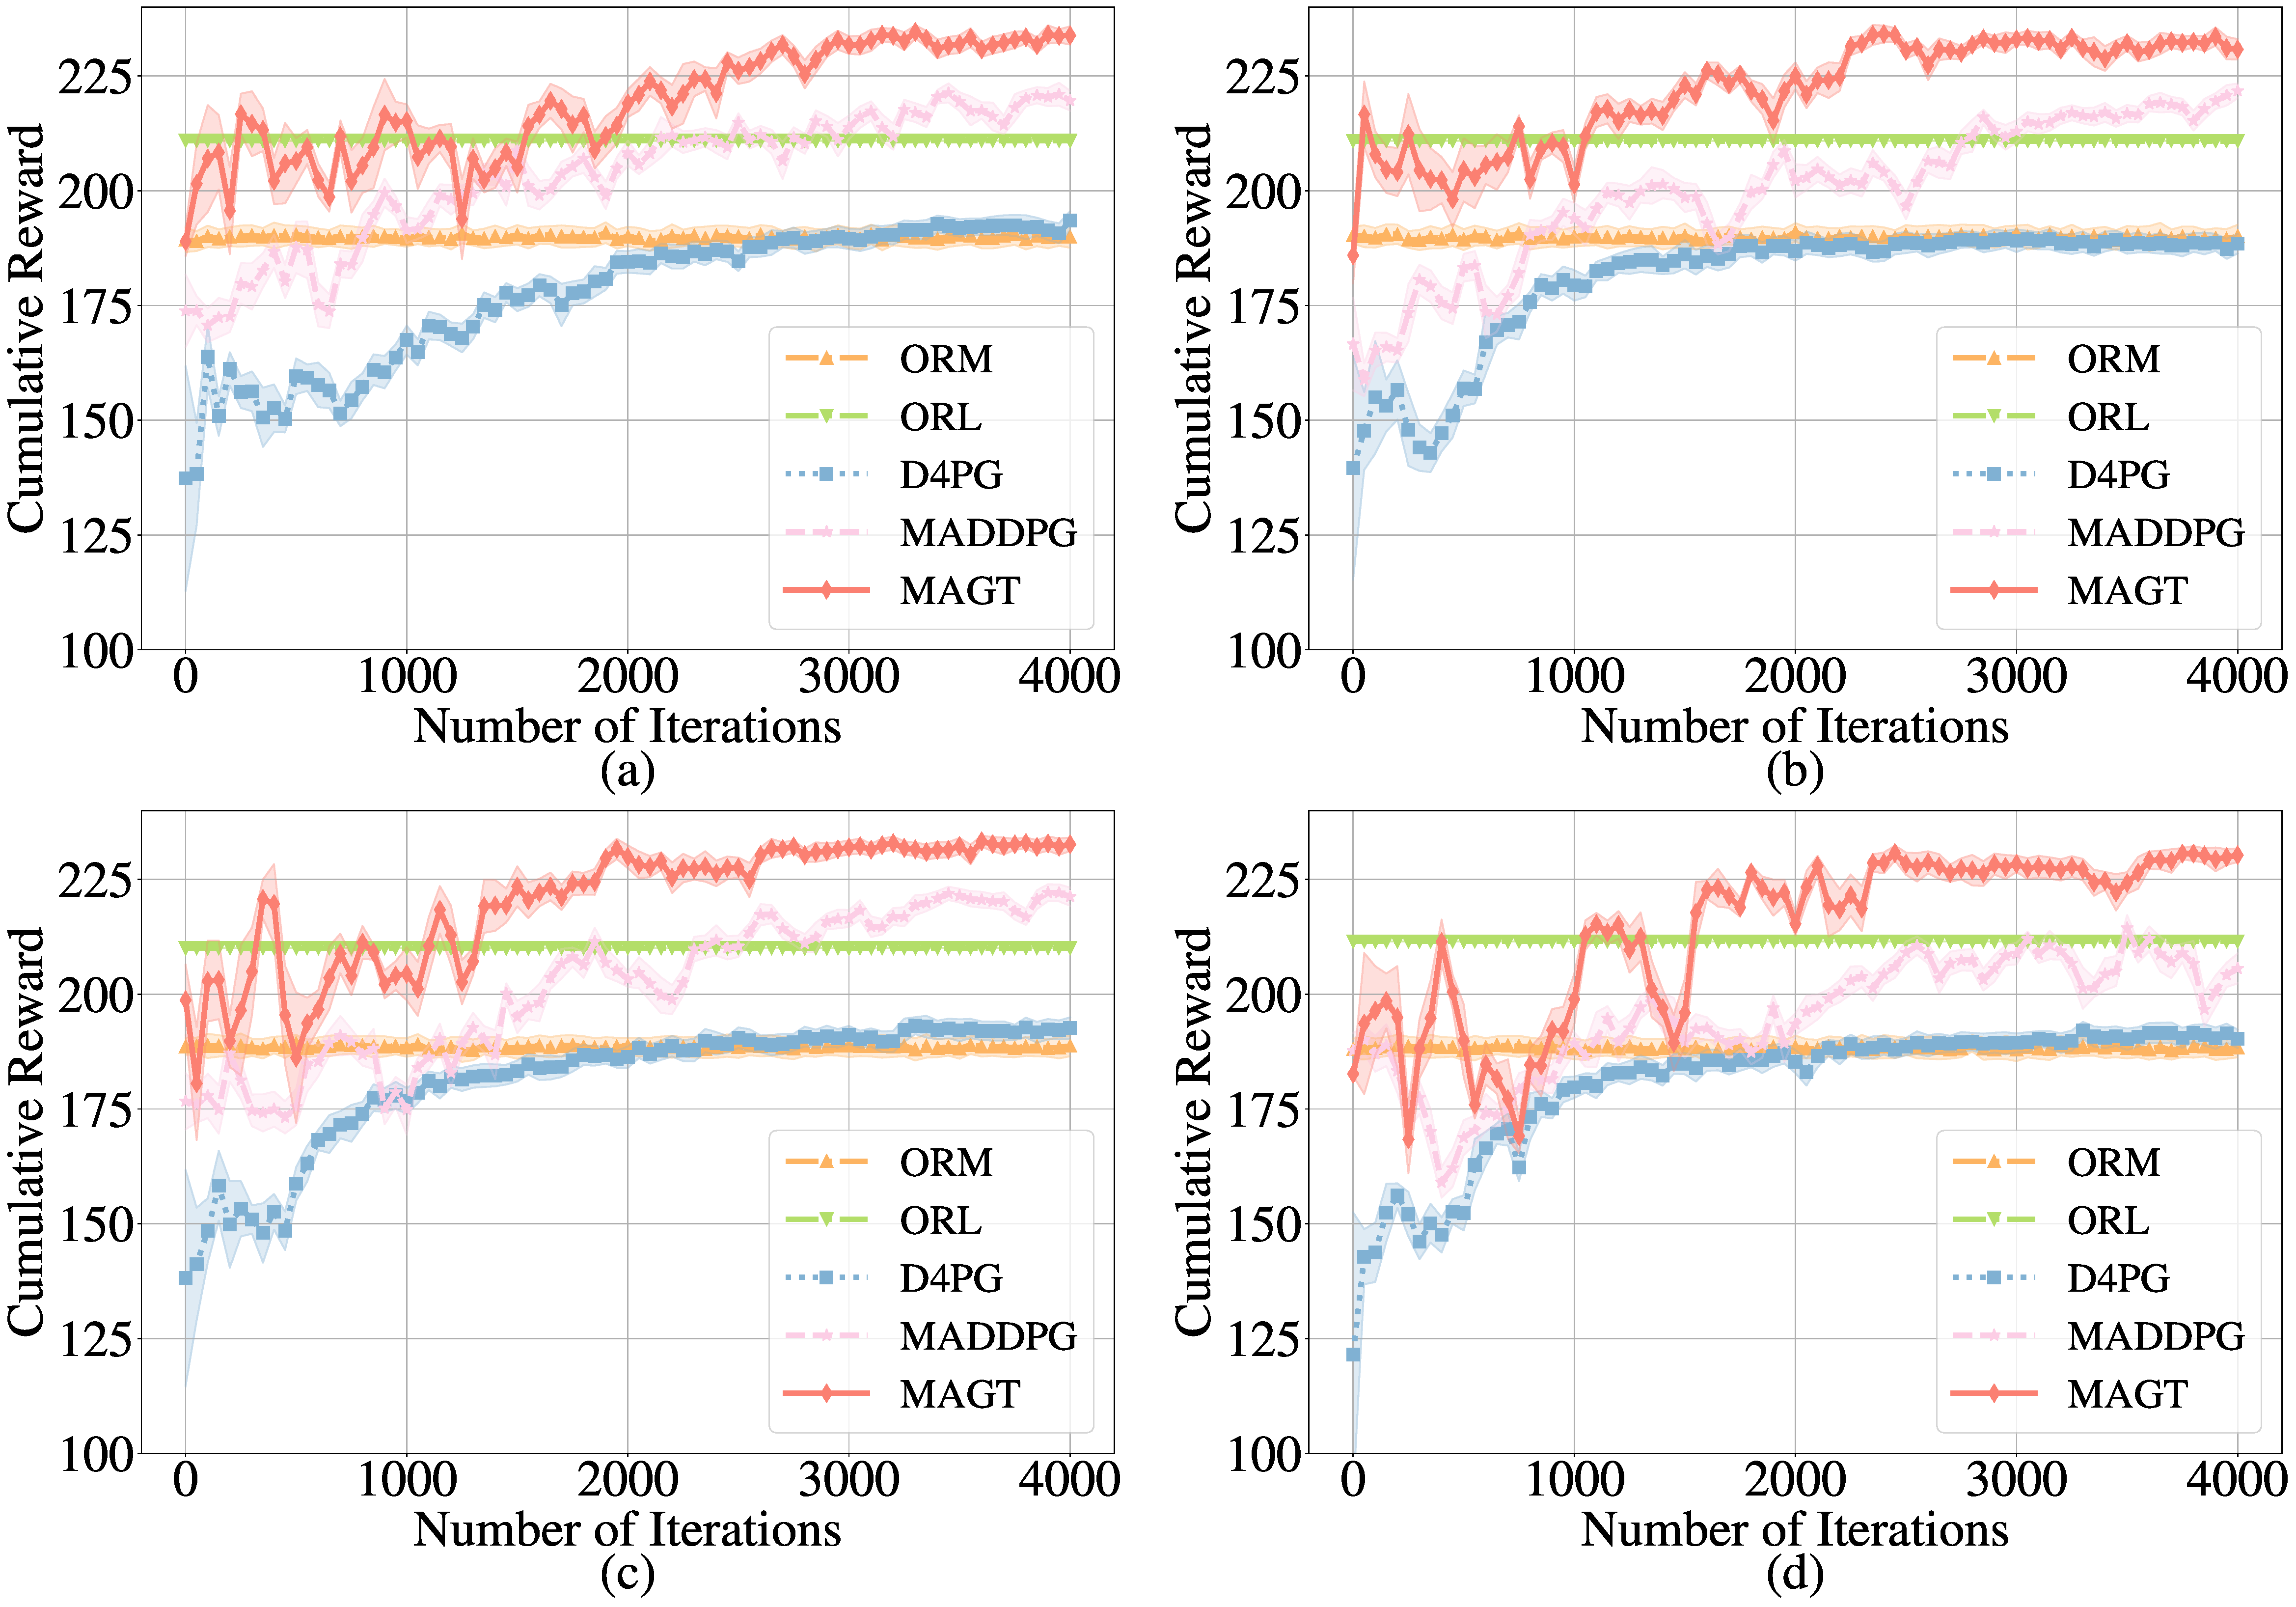
\includegraphics[width=1\columnwidth]{Fig4-4-convergence.pdf}
  \bicaption[不同交通场景下的算法收敛性]{不同交通场景下的算法收敛性。(a)场景1(b)场景2(c)场景3(d)场景4}[Algorithm convergence under different traffic scenarios]{Algorithm convergence under different traffic scenarios. (a) Scenario 1 (b) Scenario 2 (c) Scenario 3 (d) Scenario 4}
  \label{fig 3-4}
\end{figure} 

\textbf{2) 交通场景的影响:} 图\ref{fig 3-5}比较了不同交通场景下的五种算法。如图所示,图\ref{fig 3-5}(a)比较了五种算法的ASR,MAGT实现了最高的ASR。图\ref{fig 3-5}(b) 比较了五种算法的CR。如上所述,MAGT的CR高于ORM、ORL、D4PG和MADDPG。图\ref{fig 3-5}(c) 比较了五种算法的AAP。MAGT在所有场景下都能达到最高的AAP,这表明MAGT中采用势函数作为边缘节点奖励的优势。图\ref{fig 3-5}(d) and \ref{fig 3-5}(e)分别比较了五种算法的AST和APT。其表明,MAGT可以实现边缘节点之间的合作通信和计算,通过最小化任务的平均服务时间来提高整体服务率。正如预期,MAGT的APT是最低的。这可以从图\ref{fig 3-5}(f) 中得到进一步验证,图中显示任务更有可能迁移到其他边缘节点以获得更快的处理。

\begin{figure}[h]
\centering
  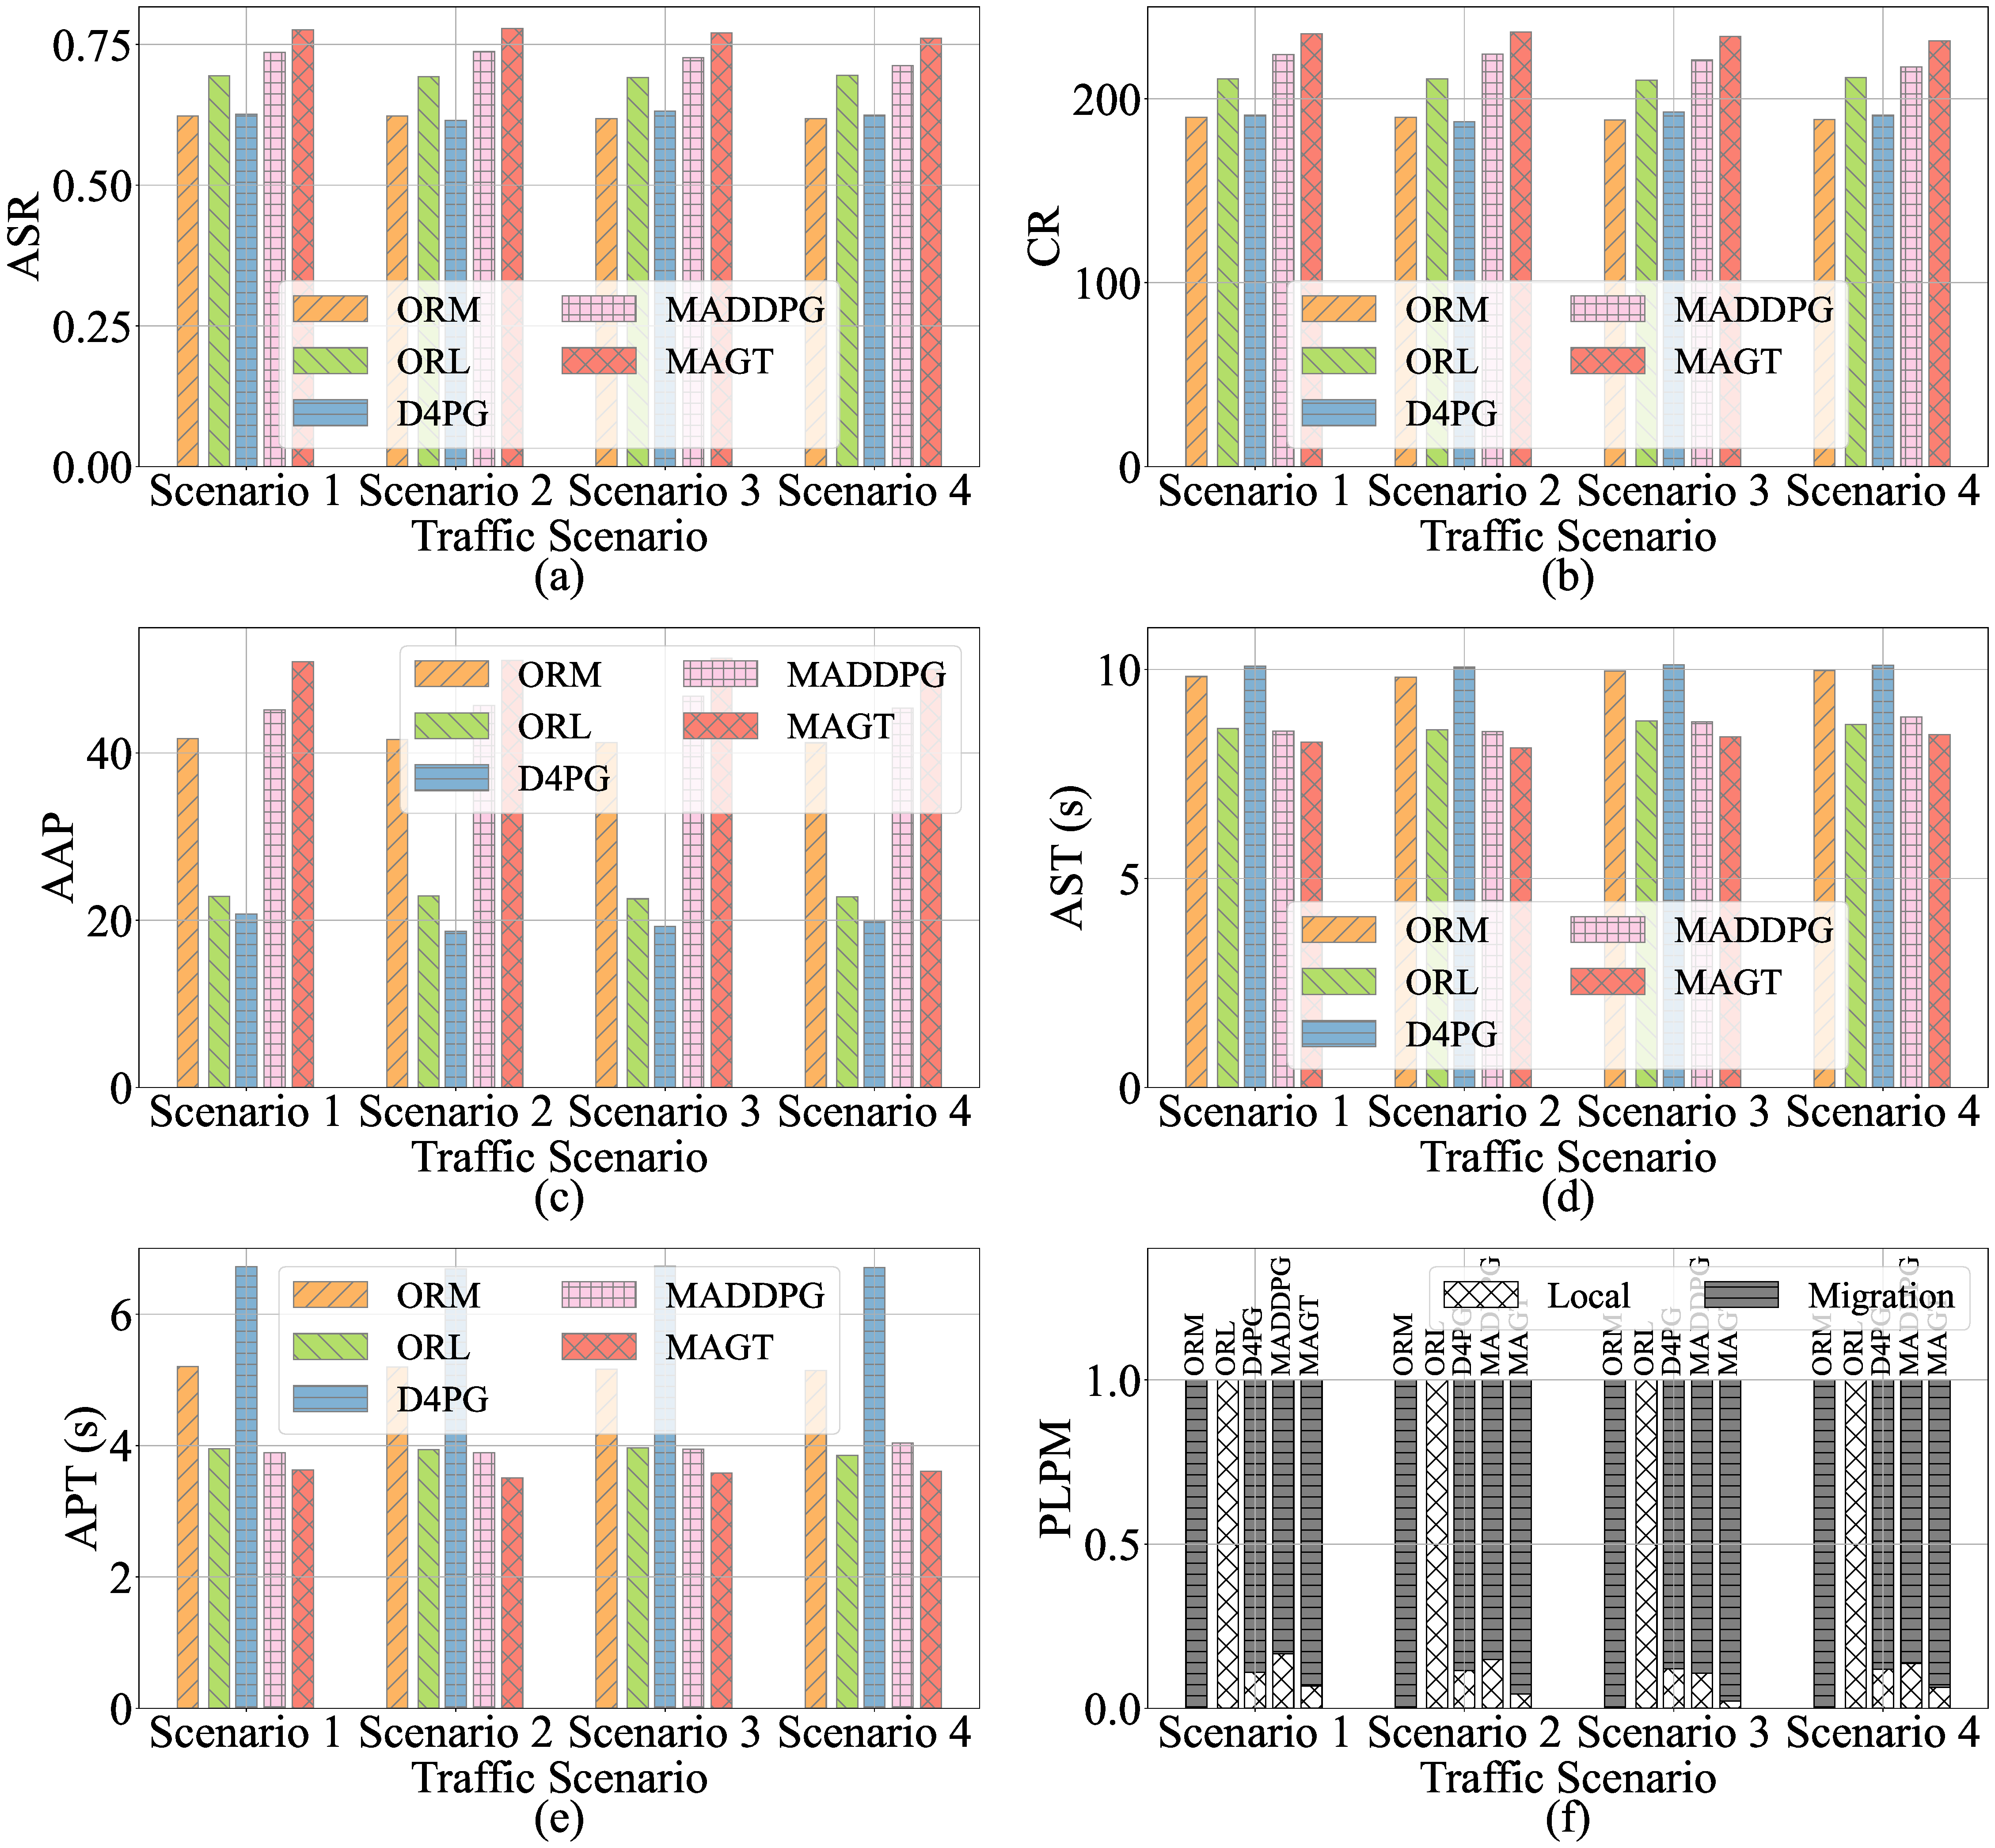
\includegraphics[width=1\columnwidth]{Fig4-5-different-traffica-scenarios.pdf}
  \bicaption[不同交通场景下的性能比较]{不同交通场景下的性能比较。(a)平均服务率(b)累积奖励(c)平均实现势(d)平均服务时间(e)平均处理时间(f)本地处理与迁移的比例}[Performance comparison under different traffic scenarios]{Performance comparison under different traffic scenarios. (a) Average service ratio (b) Cumulative reward (c) Average achieved potential (d) Average service time (e) Average processing time (f) Proportion of local processing to migration}
  \label{fig 3-5}
\end{figure}

\begin{figure}[h]
\centering
  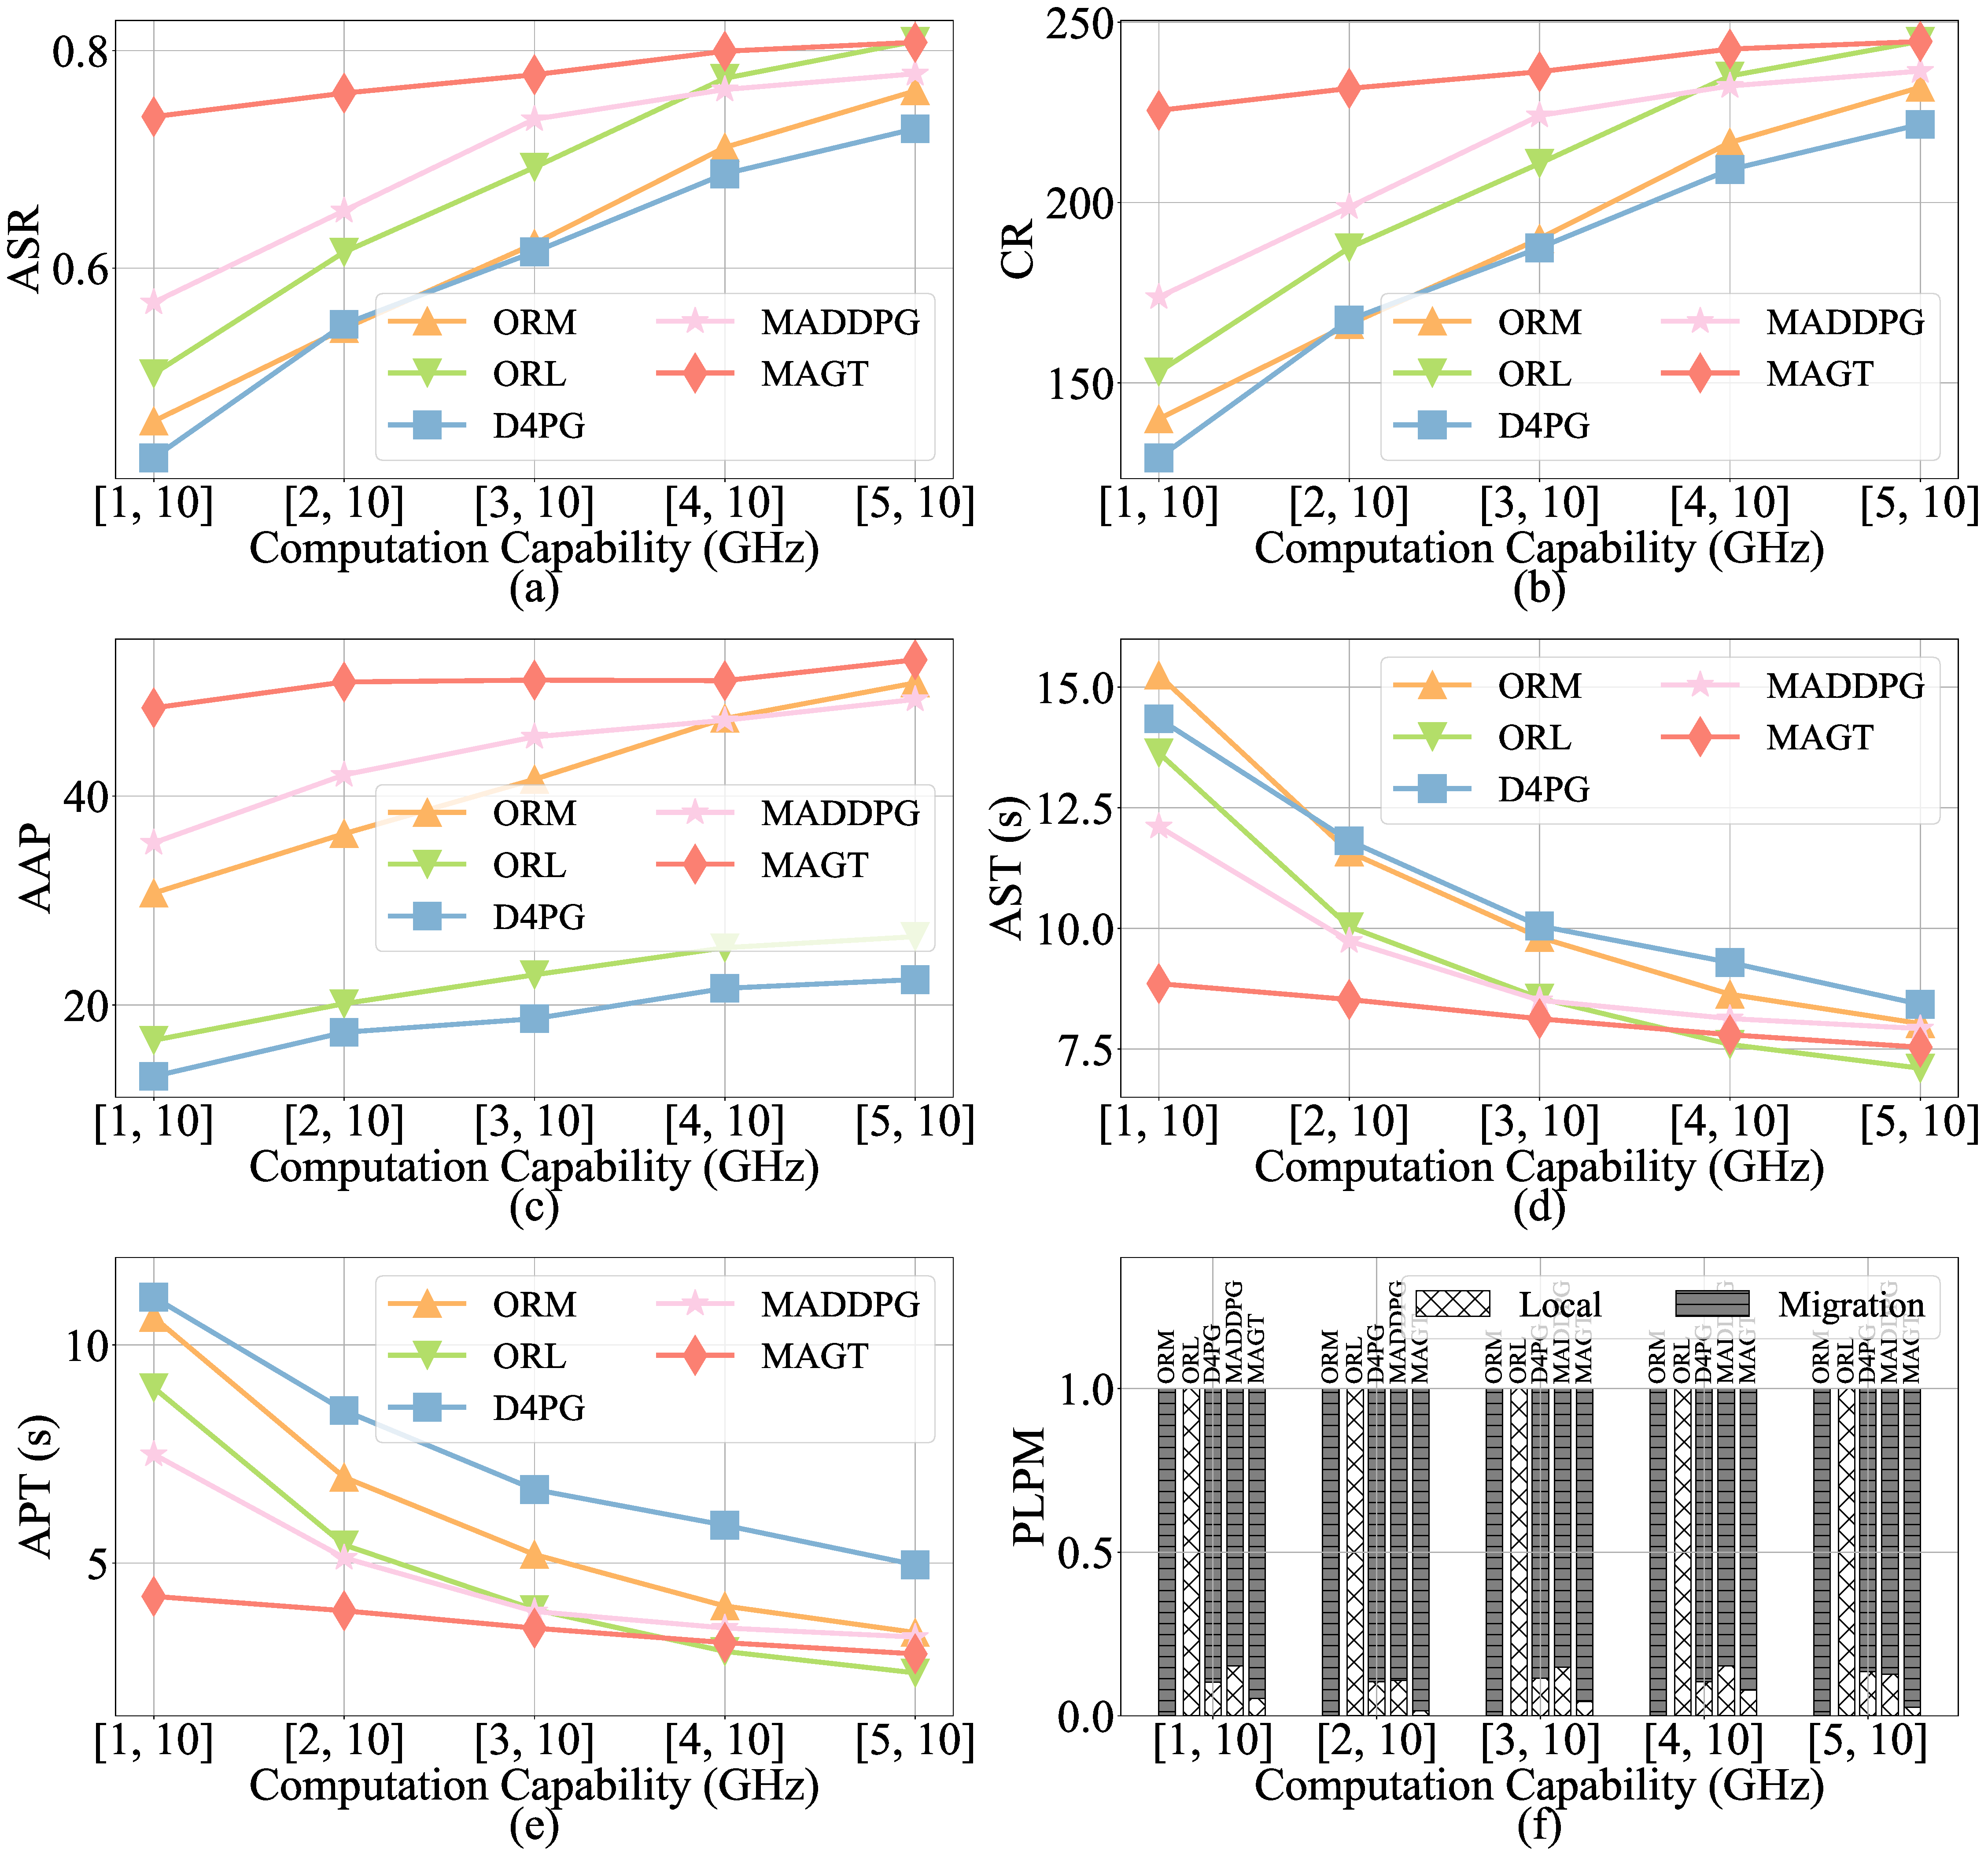
\includegraphics[width=1\columnwidth]{Fig4-6-different-computation-capability.pdf}
  \bicaption[不同边缘计算能力下的性能比较]{不同边缘计算能力下的性能比较。(a)平均服务率(b)累积奖励(c)平均实现势(d)平均服务时间(e)平均处理时间(f)本地处理与迁移的比例}[Performance comparison under different computation capabilities of edge nodes]{Performance comparison under different computation capabilities of edge nodes. (a) Average service ratio (b) Cumulative reward (c) Average achieved potential (d) Average service time (e) Average processing time (f) Proportion of local processing to migration}
  \label{fig 3-6}
\end{figure}

\textbf{3) 边缘节点计算能力的影响:} 图\ref{fig 3-6}比较了边缘节点不同计算能力下的五种算法性能。在本组实验中,边缘节点的计算能力遵循均匀分布,并从$c_e\sim[1, 10]$ GHz增加到$c_e\sim[5, 10]$ GHz,更大计算能力代表可以执行更多的任务。图\ref{fig 3-6}(a)比较了五种算法的ASR。随着计算能力的增加,所有算法的ASR都相应增加。图\ref{fig 3-6}(b) 比较了五种算法的CR。特别地,MAGT实现了最高的CR。图\ref{fig 3-6}(c)比较了五种算法的AAP。正如预期,当计算能力增加时,所有五种算法的性能都会变好。图(d)比较了五种算法的AST。本章注意到,当边缘节点的计算能力比较大时(即$c_e\sim[4,10]$ GHz和$c_e\sim[5,10]$ GHz),ORL的AST低于MAGT。原因是不同边缘节点的计算能力之间的差距变小。因此,当任务在本地执行时,任务的处理时间比卸载到其他边缘节点要短。这可以在图中进一步验证,图中显示了五种算法的APT。本章注意到,当计算能力较大时,ORL的APT是最短的;然而,ORL的ASR比MAGT要小。这是因为在MAGT中,边缘节点之间的通信和计算的合作更加有效。图\ref{fig 3-6}(f)显示了五种算法的PLPM,可以进一步确信这一优势。

\begin{figure}[h]
\centering
  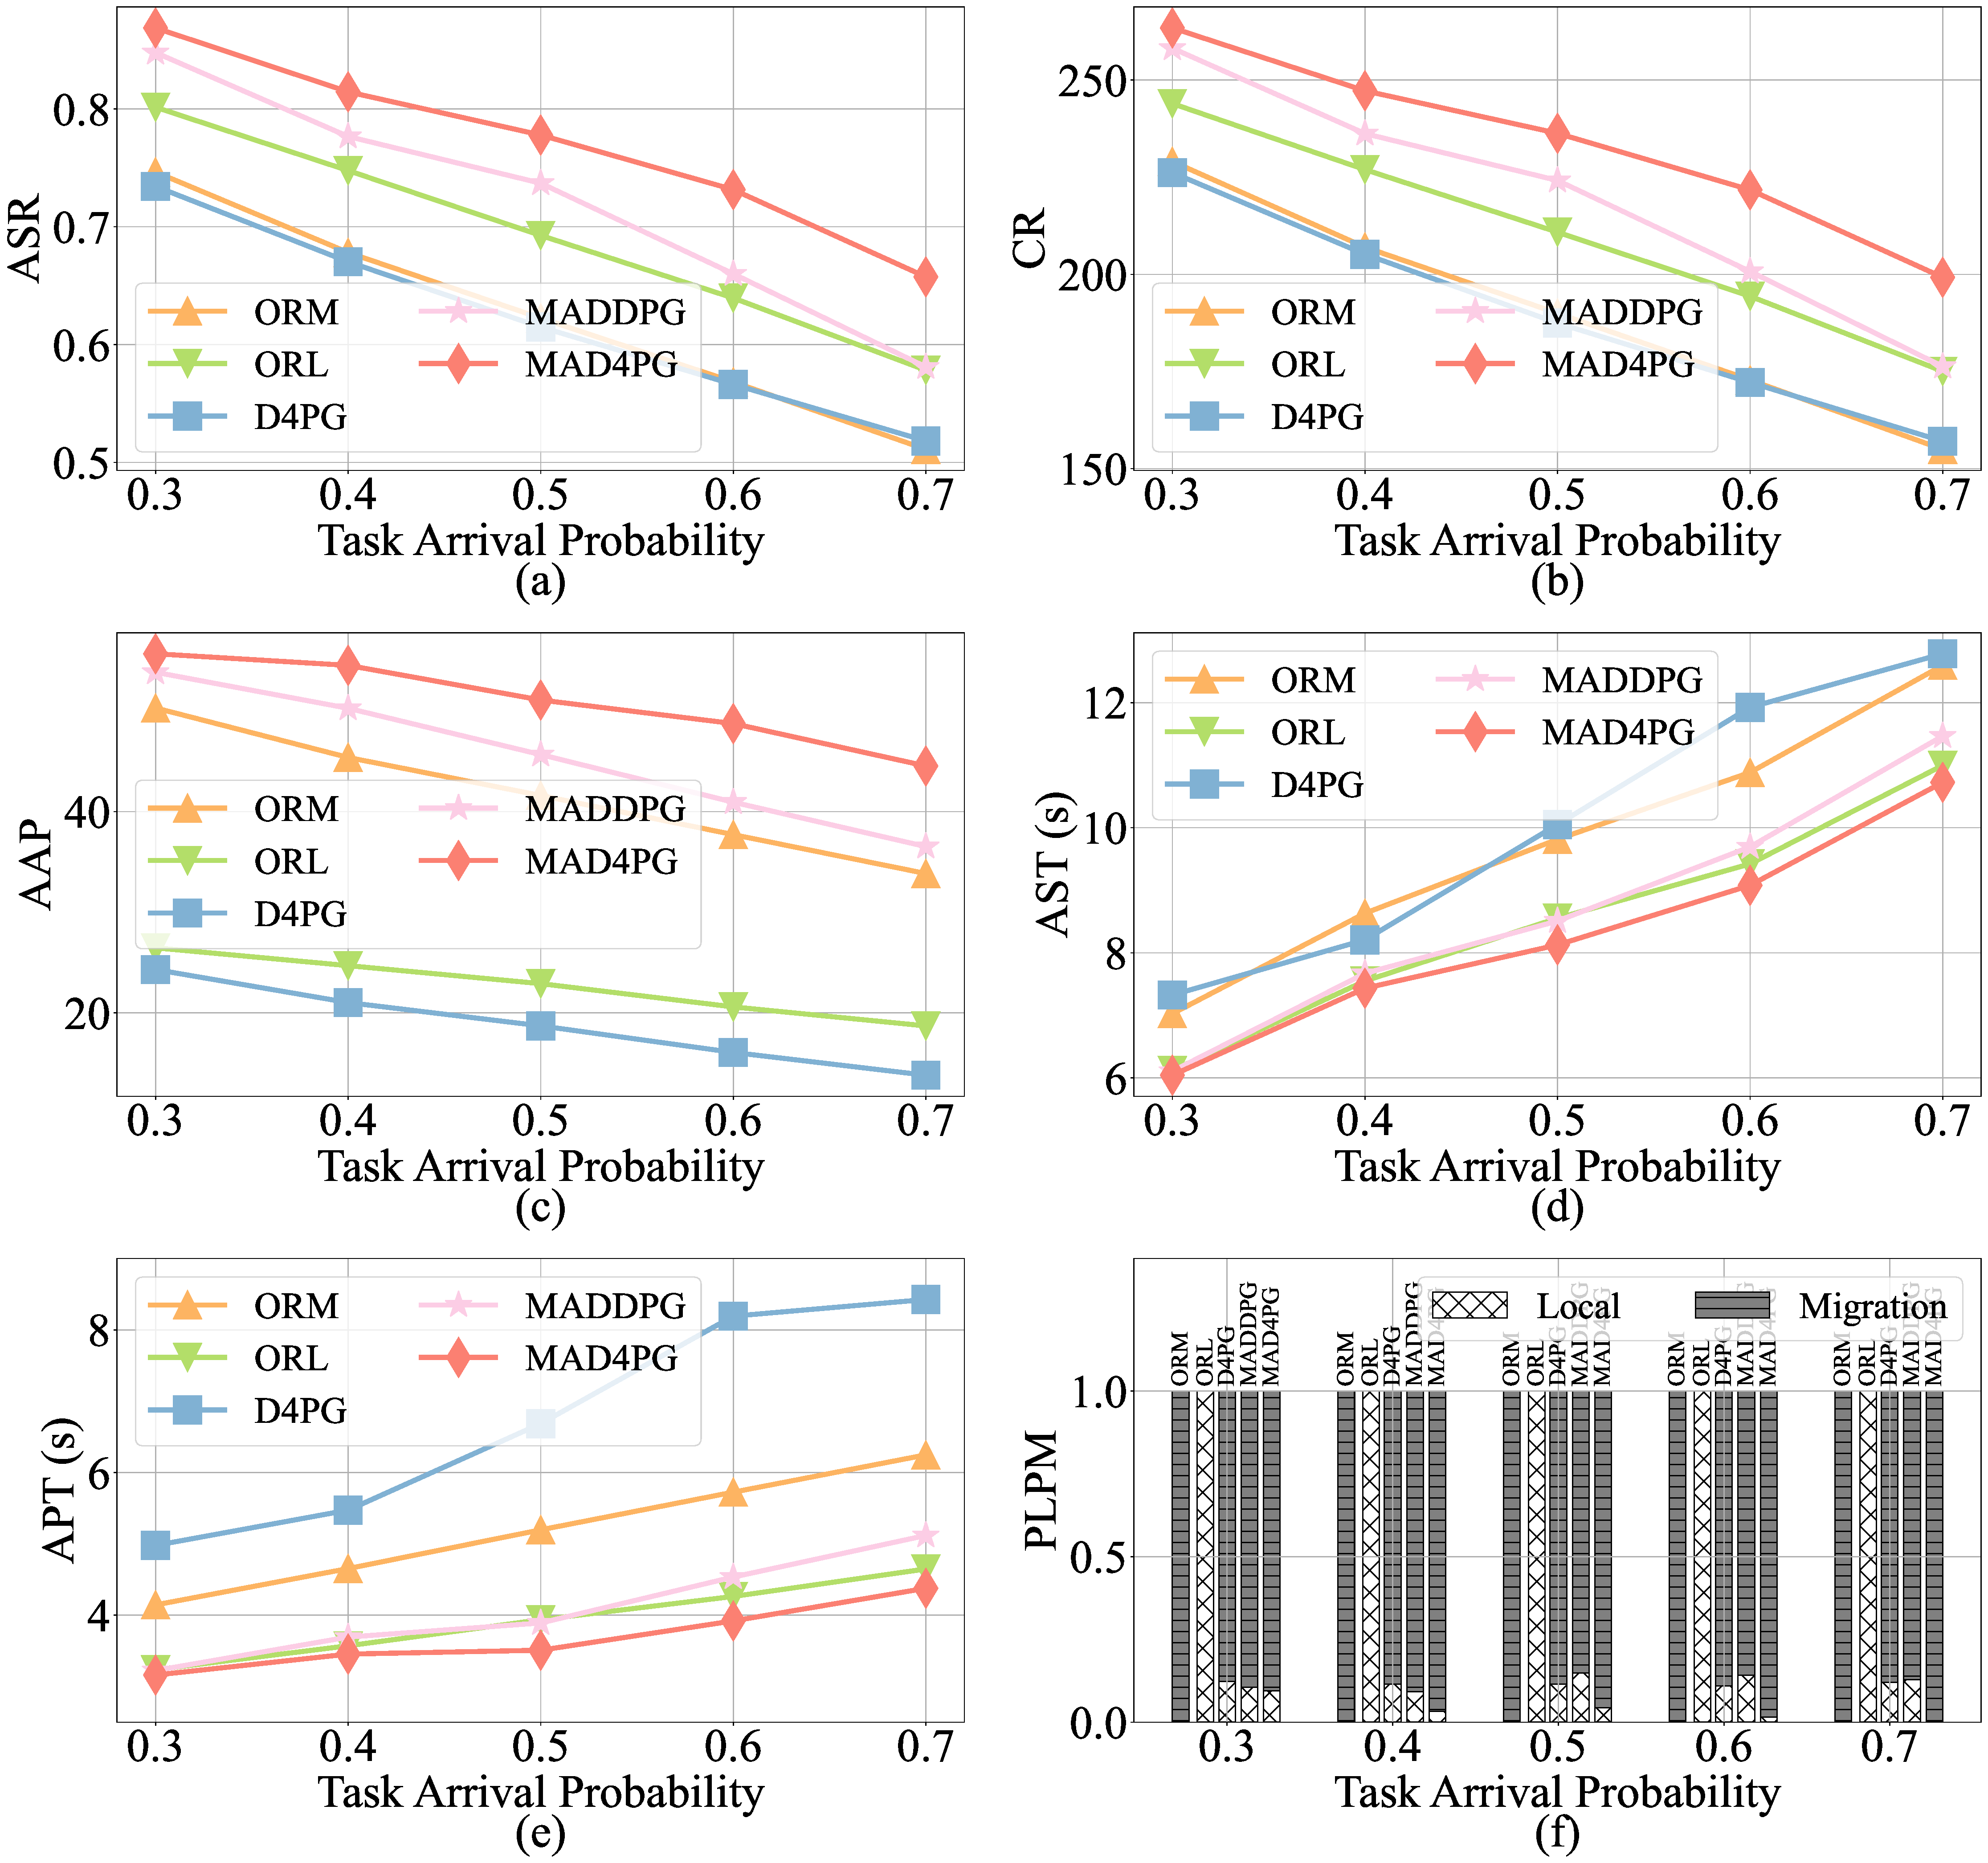
\includegraphics[width=1\columnwidth]{Fig4-7-different-task-arrival-probability.pdf}
  \bicaption[不同任务到达概率下的性能比较]{不同任务到达概率下的性能比较。(a)平均服务率(b)累积奖励(c)平均实现势(d)平均服务时间(e)平均处理时间(f)本地处理与迁移的比例}[Performance comparison under different arrival probabilities of tasks]{Performance comparison under different arrival probabilities of tasks. (a) Average service ratio (b) Cumulative reward (c) Average achieved potential (d) Average service time (e) Average processing time (f) Proportion of local processing to migration}
  \label{fig 3-7}
\end{figure} 

\textbf{4) 任务到达概率的影响:} 图\ref{fig 3-7}比较了不同车辆任务到达概率下的五种算法的性能。在本组实验中,车辆在每个时隙的任务到达概率从$\tau_{v}^{t}=0.3$增加到$\tau_{v}^{t}=0.7$。正如预期,当任务到达概率增加时,五种算法的性能都会变差。图\ref{fig 3-7}(a) 比较了五种算法的ASR,MAGT实现了最高的ASR。图\ref{fig 3-7}(b) and \ref{fig 3-7}(c) 比较五种算法的CR和AAP,显示MAGT在所有情况下都能保持最高的CR和AAP,这表明MAGT通过采用势函数作为边缘节点奖励的优势。图\ref{fig 3-7}(d) 和 图\ref{fig 3-7}(e) 比较五种算法的AST和APT。可以看出,当任务到达概率从0.3增加到0.4时,ORL、MADDPG和MAGT之间的性能差距很小。原因是,当有足够的资源时,算法的调度效果变得不明显。图\ref{fig 3-7}(f) 比较了五种算法的PLPM。当任务到达概率增加时,MAGT中本地处理的任务比例下降。原因是迁移到其他边缘节点的任务更有可能在任务截止时间前得到服务。

\section{本章小结}\label{section 3-6}

本文提出了一个基于NOMA的VEC架构,用于边缘节点之间的合作通信和计算。
在此基础上,通过考虑边缘内和边缘间干扰的建立了V2I传输模型,并通过考虑异构资源和边缘节点间的合作建立了任务卸载模型。
然后,本章提出了CRO问题,其目标为最大化任务服务率。
此外,本章将CRO分解为两个子问题,即任务卸载和资源分配。
任务卸载子问题被建模为一个具有NE存在和收敛性的EPG。
提出了MAGT算法,其中边缘节点作为智能体,在行动空间中决定任务卸载策略以实现NE。
特别地,博弈模型的势函数被作为边缘节点的奖励。
然后,根据基于梯度的迭代方法和KKT条件,提出了解决资源分配问题的最优方案。
最后,本章利用从不同时期提取的真实车辆轨迹建立了仿真模型,并通过综合性能评估证明了所提方案的优越性。

\chapter[面向车载信息物理融合的质量-开销均衡优化关键技术]{面向车载信息物理融合的质量-开销均衡优化关键技术}

本章主要研究面向车载信息物理融合的质量-开销均衡优化关键技术。
具体内容安排如下:
\ref{section 4-1} 节是本章的引言,介绍车联网中车载信息物理融合系统的研究现状及存在的不足,同时阐述本章的主要贡献。
\ref{section 4-2} 节阐述协同感知与V2I上传场景。
\ref{section 4-3} 节给出了系统模型的详细描述。
\ref{section 4-4} 节形式化定义了最大化VCPS质量并最小化VCPS开销的双目标优化问题。
\ref{section 4-5} 节设计了基于多目标的多智能体深度强化学习算法。
\ref{section 4-6} 节搭建了实验仿真模型并进行了性能验证。
\ref{section 4-7} 节对本章的研究工作进行总结。

\section{引言}\label{section 4-1}

最新的感知技术、无线通信和计算模式推动了现代新能源汽车和智能网联汽车的发展。现代汽车中装备了各种车载感知器,以增强车辆的环境感知能力 \cite{zhu2017overview}。另一方面,V2X通信\cite{chen2020a}的发展使车辆、路侧设备和云端之间的合作得以实现。同时,车载边缘计算\cite{dai2021edge}是一个很有前途的范式,可以实现计算密集型和延迟关键型的智能交通系统应用 \cite{zhao2022foundation}。这些进展都成为了开发车载信息物理融合系统的强大驱动力。具体来说,通过协同感知和上传,车联网中的物理实体,如车辆、行人和路侧设备等,可以在边缘节点上构建为相应的逻辑映射。

车载信息物理融合中的检测、预测、规划和控制技术被广泛研究。大量工作聚焦于检测技术,例如雨滴数量检测\cite{wang2021deep}和驾驶员疲劳检测\cite{chang2018design}。针对车辆状态预测方法,研究人员提出了混合速度曲线预测\cite{zhang2019a}、车辆跟踪\cite{iepure2021a}和加速预测\cite{zhang2020data}等。同时,部分研究工作提出了不同的调度方案,例如基于物理比率-K干扰模型的广播调度\cite{li2020cyber}和基于既定地图模型的路径规划\cite{lian2021cyber}。此外,部分研究集中在智能网联车辆的控制算法上,例如车辆加速控制\cite{lv2018driving}、交叉路口控制\cite{chang2021an}和电动汽车充电调度\cite{wi2013electric}。这些关于状态检测、轨迹预测、路径调度和车辆控制的研究促进了各种ITS应用的实施。然而,这些工作忽略了感知和上传开销,假设高质量可用信息可以在VEC中构建。少数研究考虑了VCPS中的信息质量,例如时效性\cite{liu2014temporal, dai2019temporal}和准确性\cite{rager2017scalability, yoon2021performance},但上述研究都没有考虑通过协同感知和上传,在VCPS中实现高质量低成本的信息物理融合。

本章旨在通过车辆协同感知与上传,构建基于车载信息物理融合的逻辑视图,并进一步在最大化车载信息物理融合质量和最小化视图构建开销方面寻求最佳平衡。然而,实现这一目标面临着以下主要挑战。首先,车联网中的信息高度动态,因此考虑感知频率、排队延迟和传输时延的协同效应,以确保信息的新鲜度和时效性是至关重要的。其次,物理信息是具有时空相关性的,不同车辆在不同的时间或空间范围内感应到的信息可能存在冗余或不一致性。因此,具有不同感知能力的车辆有望以分布式方式合作,以提高感知和通信资源的利用率。再次,物理信息在分布、更新频率和模式方面存在异质性,这给构建高质量视图带来很大挑战。最后,高质量的视图构建需要更高的感知和通信资源开销,这也是一个需要考虑的关键因素。综上所述,通过协同感知和上传,实现面向车载边缘计算的高质量、低开销视图具有重要意义,但也具有一定的挑战性。

本章致力于研究车载信息物理融合系统的质量-开销均衡优化问题,并通过协同感知与上传实现高质量、低开销的视图建模。本章的主要贡献如下:第一,提出了协同感知与V2I上传场景,考虑视图的及时性和一致性,设计了车载信息物理融合质量指标,并考虑边缘视图构建过程中信息冗余度、感知开销和传输开销,设计了车载信息物理融合开销指标。进一步,提出了一个双目标优化问题,在最大化VCPS质量的同时最小化VCPS开销。第二,提出了基于多目标的多智能体深度强化学习算法(Multi-Agent Multi-Objective Deep Reinforcement Learning, MAMO)。具体地,在车辆和边缘节点中分别部署智能体,车辆动作空间包括感知决策、感知频率、上传优先级和传输功率分配,而边缘节点动作空间是V2I带宽分配策略。同时,设计了决斗评论家网络(Dueling Critic Network, DCN),其根据状态价值(State-Value, SV)和动作优势(Action-Advantage, AA)评估智能体动作。系统奖励是一个一维向量,其中包含VCPS质量和VCPS利润,并通过差分奖励信用分配得到车辆的个人奖励,进一步通过最小-最大归一化得到边缘节点的归一化奖励。第三,建立了基于现实世界车辆轨迹的仿真实验模型,并将MAMO与三种对比算法进行比较,包括随机分配、分布式深度确定性策略梯度\cite{barth2018distributed},以及多智能体分布式深度确定性策略梯度。此外,本文设计了两个指标,即单位开销质量(Quality Per Unit Cost, QPUC)和单位质量利润(Profit Per Unit Quality, PPUQ)用于定量衡量算法实现的均衡。仿真结果表明,与其他算法相比,MAMO在最大化QPUC和PPUQ方面更具优势。

\section{协同感知与 V2I 上传场景}\label{section 4-2}

本章节介绍了协同感知与V2I上传场景。如图\ref{fig 4-1}所示,车辆配备各种车载感知器,如超声波雷达、激光雷达、光学相机和毫米波雷达,可以对环境进行感知。通过车辆间协同地感知,可以获得异质信息,包括其他车辆、弱势道路参与者、停车场和路边基础设施的状态。这些信息可用于在边缘节点中建立视图模型,并进一步用于支撑各种ITS应用,如自动驾驶\cite{bai2022hybrid}、智慧路口控制系统\cite{hadjigeorgious2023real},以及全息城市交通流管理\cite{wang2023city}。逻辑视图需要融合车联网中物理实体的不同模式信息,以更好地反映实时物理车辆环境,从而提高ITS的性能。然而,构建高质量的逻辑视图可能需要更高的感知频率、更多的信息上传量以及更高的能量消耗。

本系统的工作流程如下:首先,车辆感知并排队上传不同物理实体的实时状态。接着,边缘节点将V2I带宽分配给车辆,同时,车辆确定传输功率。物理实体的视图是基于从车辆收到的异质信息进行融合建立的。需要注意的是,在该系统中,异质信息是由车辆以不同的感知频率感应到的,因此上传时的新鲜度会不同。虽然增加感知频率可以提高新鲜度,但会增加排队延迟和能源消耗。此外,多个车辆可能感知到特定物理实体的信息,若由所有车辆上传,则可能会浪费通信资源。因此,为了提高资源利用率,需要有效而经济地分配通信资源。在此基础上,为了最大化面向车载边缘计算的视图的VCPS质量并最小化VCPS开销,必须量化衡量边缘节点构建的视图的质量和开销,并设计高效经济的协同感知和上传的调度机制。

\begin{figure}[h]
\centering
  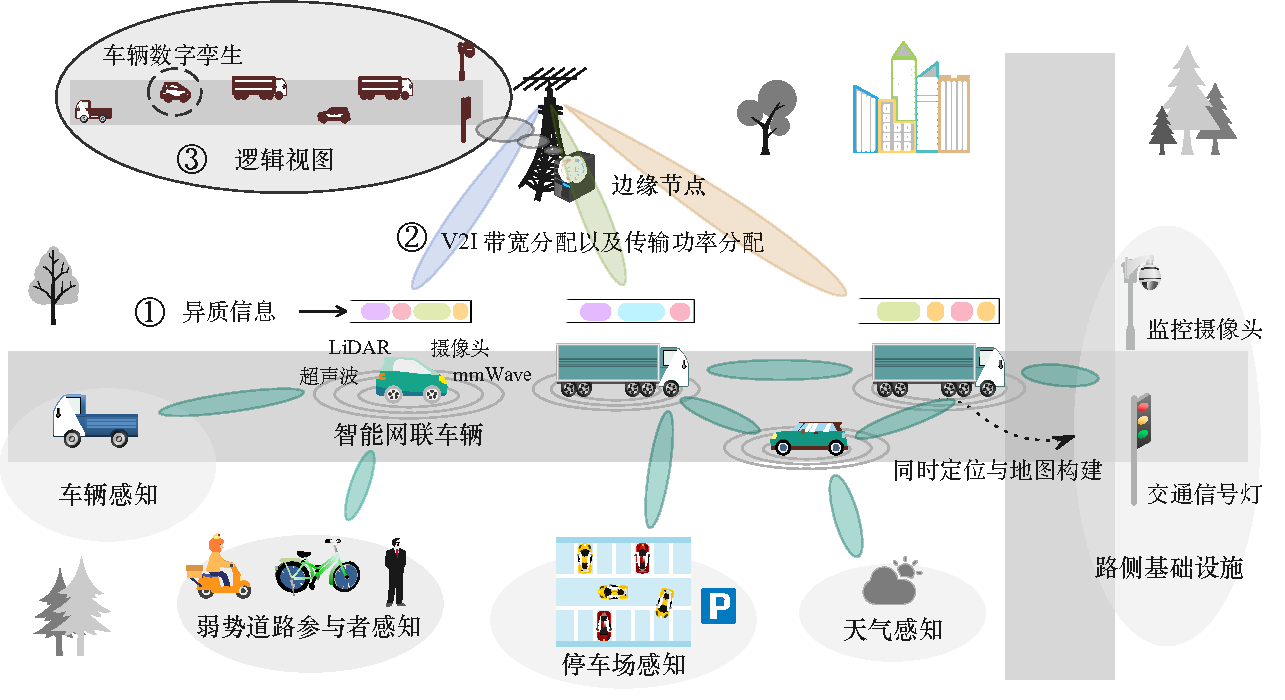
\includegraphics[width=1\columnwidth]{Fig4-1-architerture.pdf}
  \bicaption{协同感知与 V2I 上传场景}{Cooperative sensing and V2I uploading scenario}
  \label{fig 4-1}
\end{figure} 

\section{车载信息物理融合质量/开销模型}\label{section 4-3}
\subsection{基本符号}
本系统离散时间片的集合用$\mathbf{T}=\left\{1,\ldots,t,\ldots, T \right\}$表示。
异质信息集合用$\mathbf{D}$表示,其中信息$d \in \mathbf{D}$的特征是一个三元组$d=\left(\operatorname{type}_d, u_d, \left|d\right| \right)$,其中$\operatorname{type}_d$、$u_d$和$\left|d\right|$分别是信息类型、更新间隔和数据大小。
$\mathbf{V}$表示车辆的集合,每个车辆$v\in \mathbf{V}$的特征是一个三元组$v=\left (l_v^t, \mathbf{D}_v, \pi_v \right )$,其中$l_v^t$、$\mathbf{D}_v$和$\pi_v$分别是位置、感知的信息集和传输功率。
对于$d \in \mathbf{D}_v$,车辆$v$的感知开销(即能耗)用$\phi_{d, v}$表示。
用$\mathbf{E}$表示边缘节点的集合,其中每个边缘节点$e \in \mathbf{E}$的特征是$e=\left (l_e, g_e, b_e \right)$,其中$l_{e}$、$r_{e}$和$b_{e}$分别为位置、通信范围和带宽。
车辆$v$与边缘节点$e$之间的距离表示为$\operatorname{dis}_{v, e}^t \triangleq \operatorname{distance} \left (l_v^t, l_e \right ), \forall v \in \mathbf{V}, \forall e \in \mathbf{E}, \forall t \in \mathbf{T}$。
在时间$t$内处于边缘节点$e$的通信覆盖范围内的车辆集合表示为$\mathbf{V}_e^t=\left \{v \vert \operatorname{dis}_{v, e}^t \leq g_e, \forall v \in \mathbf{V} \right \}, \mathbf{V}_e^t \subseteq \mathbf{V}$。

感知决策指示器表示车辆$v$在时间$t$是否感知信息$d$,其用以下方式表示:
\begin{equation}
	c_{d, v}^t \in \{0, 1\}, \forall d \in \mathbf{D}_{v}, \forall v \in \mathbf{V}, \forall t \in \mathbf{T}
	\label{equ 4-1} 
\end{equation}
那么,车辆$v$在时间$t$的感应信息集合表示为 $\mathbf{D}_v^t = \{ d | c_{d, v}^{t} = 1, \forall d \in \mathbf{D}_v \}, \mathbf{D}_v^t \subseteq \mathbf{D}_v$。
对于任何信息$d \in \mathbf{D}_v^t$来说,信息类型都是不同的, 即$\operatorname{type}_{d^*} \neq \operatorname{type}_{d}, \forall d^* \in \mathbf{D}_v^t \setminus \left\{ d\right \}, \forall d \in \mathbf{D}_v^t$。
车辆$v$在时间$t$的信息$d$的感知频率用$\lambda_{d, v}^t$表示,其需要满足车辆$v$的感应能力要求。
\begin{equation}
	\lambda_{d, v}^{t} \in [\lambda_{d, v}^{\min} , \lambda_{d, v}^{\max} ], \ \forall d \in \mathbf{D}_v^t, \forall v \in \mathbf{V}, \forall t \in \mathbf{T}
\end{equation}
其中$\lambda_{d, v}^{\min}$和$\lambda_{d, v}^{\max}$分别是车辆$v$中信息${d}$的最小和最大感知频率。
车辆$v$中的信息$d$在时间$t$的上传优先级用$p_{d, v}^t$表示,不同信息的上传优先级需各不相同。
\begin{equation}
	{p}_{d^*, v}^t \neq {p}_{d, v}^t, \forall d^* \in \mathbf{D}_v^t \setminus \left\{ d\right \}, \forall d \in \mathbf{D}_v^t, \forall v \in \mathbf{V}, \forall t \in \mathbf{T}
\end{equation}
其中${p}_{d^*, v}^t$是信息$d^* \in \mathbf{D}_v^t$中的上传优先级。
车辆$v$在时间$t$的传输功率用$\pi_{v}^t$表示,其不能超过车辆$v$的功率容量。
\begin{equation}
	\pi_v^t \in \left[ 0 , \pi_v \right ], \forall v \in \mathbf{V}, \forall t \in \mathbf{T}
\end{equation}
边缘节点$e$在时间$t$为车辆$v$分配的V2I带宽用$b_{v, e}^t$表示,且其需要满足:
\begin{equation}
	b_{v, e}^t \in \left [0, b_e \right], \forall v \in \mathbf{V}_e^{t}, \forall e \in \mathbf{E}, \forall t \in \mathbf{T}
	\label{equ 4-5} 
\end{equation}
边缘节点$e$分配的V2I总带宽不能超过其容量$b_e$,即${\sum_{\forall v \in \mathbf{V}_e^{t}} b_{v, e}^t} \leq b_e, \forall t \in \mathbf{T}$。

本系统中物理实体的集合为 $\mathbf{I}^{\prime}$,其中$i^{\prime} \in \mathbf{I}^{\prime}$表示物理实体,如车辆、行人和路侧基础设施等。
$\mathbf{D}_{i^{\prime}}$是与实体$i^{\prime}$相关的信息集合,可以用$\mathbf{D}_{i^{\prime}}=\left\{d \mid y_{d, i^{\prime}} = 1, \forall d \in \mathbf{D} \right\}$, $\forall i^{\prime} \in \mathbf{I}^{\prime}$表示, 其中$y_{d, i^{\prime}}$是一个二进制数,表示信息$d$是否与实体$i^{\prime}$关联。
$\mathbf{D}_{i^{\prime}}$的大小用$|\mathbf{D}_{i^{\prime}}|$表示。
每个实体可能需要多个信息,即$|\mathbf{D}_{i^{\prime}}| = \sum_{\forall d \in \mathbf{D}}y_{d, i^{\prime}} \geq 1, \forall i^{\prime} \in \mathbf{I}^{\prime}$。
对于每个实体$i^{\prime} \in \mathbf{I}^{\prime}$,可能有一个视图$i$在边缘节点中建模。
用$\mathbf{I}$表示视图的集合,用$\mathbf{I}_e^{t}$表示时间为$t$时在边缘节点$e$中建模的视图集合。
因此,边缘节点$e$收到且被视图$i$需要的信息集合可以用$\mathbf{D}_{i, e}^t=\bigcup_{\forall v \in \mathbf{V}}\left(\mathbf{D}_{i^{\prime}} \cap \mathbf{D}_{v, e}^t\right), \forall i \in \mathbf{I}_e^{t}, \forall e \in \mathbf{E}$表示,且 $| \mathbf{D}_{i, e}^t |$是边缘节点$e$收到且被视图$i$需要的信息数量,其计算公式为$| \mathbf{D}_{i, e}^t | =  \sum_{\forall v \in \mathbf{V}} \sum_{\forall d \in \mathbf{D}_v} c_{d, v}^t  y_{d, i^{\prime}}$。

\subsection{协同感知模型}
车辆协同感知是基于多类M/G/1优先级队列\cite{moltafet2020age}进行建模。
假设具有$\operatorname{type}_d$的信息的上传时间$\operatorname{\hat{g}}_{d, v, e}^t$遵循均值$\alpha_{d, v}^t$和方差$\beta_{d, v}^t$的一类一般分布。
那么,车辆$v$中的上传负载$\rho_{v}^{t}$由$ \rho_{v}^{t}=\sum_{\forall d \subseteq \mathbf{D}_v^t} \lambda_{d, v}^{t} \alpha_{d, v}^t$表示。
根据多类M/G/1优先级队列,需要满足$\rho_{v}^{t} < 1$才能达到队列的稳定状态。
信息$d$在时间$t$之前的到达时间用$\operatorname{a}_{d, v}^t$表示,其计算公式为:
\begin{equation}
    \operatorname{a}_{d, v}^t =  \frac{\left \lfloor t \lambda_{d, v}^t \right \rfloor }{\lambda_{d, v}^{t}} 
\end{equation}
在时间$t$之前,由$\operatorname{u}_{d, v}^t$表示的信息$d$的更新时间是通过下式计算:
\begin{equation}
    \operatorname{u}_{d, v}^t = \left \lfloor  \frac{\operatorname{a}_{d, v}^t}{u_d} \right \rfloor  u_d
\end{equation}
其中$u_d$是信息$d$的更新间隔时间。


在时间$t$,车辆$v$中比$d$有更高上传优先级的信息集合,用$\mathbf{D}_{d, v}^t = \{ d^* \mid p_{d^*, v}^{t} > p_{d, v}^{t} , \forall d^* \in \mathbf{D}_v^t \}$表示,其中$p_{d^*, v}^{t}$是信息$d^* \in \mathbf{D}_v^t$的上传优先级。
因此,信息$d$前面的上传负载(即$v$在时间$t$时要在$d$之前上传的信息数量)通过下方计算得出: 
\begin{equation}
	\rho_{d, v}^{t}=\sum_{\forall d^* \in \mathbf{D}_{d, v}^t} \lambda_{d^*, v}^t \alpha_{d^*, v}^t
\end{equation}
其中$\lambda_{d^*, v}^t$和$\alpha_{d^*, v}^t$分别为时间$t$内车辆$v$中信息$d^*$的感知频率和平均传输时间。
根据Pollaczek-Khintchine公式\cite{takine2001queue},车辆$v$中信息$d$的排队时间计算如下:
\begin{equation}
    \operatorname{q}_{d, v}^t= \frac{1} {1 - \rho_{d, v}^{t}} 
        \left[ \alpha_{d, v}^t + \frac{ \lambda_{d, v}^{t} \beta_{d, v}^t + \sum\limits_{\forall d^* \in \mathbf{D}_{d, v}^t} \lambda_{d^*, v}^t \beta_{d^*, v}^t }{2\left(1-\rho_{d, v}^{t} - \lambda_{d, v}^{t} \alpha_{d, v}^t\right)}\right] 
        - \alpha_{d, v}^t
\end{equation}

\subsection{V2I协同上传模型}
车辆间V2I协同上传是基于信道衰减分布和信噪比阈值来建模的。
车辆$v$和边缘节点$e$之间的V2I通信在时间$t$的信噪比通过公式\ref{equ 4-10}\cite{sadek2009distributed}计算得到。
\begin{equation}
    \operatorname{SNR}_{v, e}^{t}=\frac{1}{N_{0}} \left|h_{v, e}\right|^{2} \tau {\operatorname{dis}_{v, e}^{t}}^{-\varphi} {\pi}_v^t
    \label{equ 4-10}
\end{equation}
其中$N_{0}$为AWGN;$h_{v, e}$为信道衰减增益;$\tau$为取决于天线设计的常数;$\varphi$为路径损耗指数。
假设$\left|h_{v, e}\right|^{2}$遵循均值$\mu_{v, e}$和方差$\sigma_{v, e}$的一类分布,其表示方法为:
\begin{equation}
    \tilde{p}=\left\{\mathbb{P}: \mathbb{E}_{\mathbb{P}}\left[\left|h_{v, e}\right|^{2}\right]=\mu_{v, e}, \mathbb{E}_{\mathbb{P}}\left[\left|h_{v, e}\right|^{2}-\mu_{v, e}\right]^{2}=\sigma_{v, e}\right\}
\end{equation}
进一步,基于成功传输概率和可靠性阈值来衡量V2I传输可靠性。
\begin{equation}
    \inf_{\mathbb{P} \in \tilde{p}} \operatorname{Pr}_{[\mathbb{P}]}\left(\operatorname{SNR}_{v, e}^{t} \geq \operatorname{SNR}_{v, e}^{\operatorname{tgt}}\right) \geq \delta
\end{equation}
\noindent 其中$\operatorname{SNR}_{v, e}^{\operatorname{tgt}}$和$\delta$分别为目标SNR阈值和可靠性阈值。
由车辆$v$上传并由边缘节点$e$接收的信息集合用$\mathbf{D}_{v, e}^{t} = \bigcup_{\forall v \in \mathbf{V}_{e}^{t}} \mathbf{D}_{v}^{t}$表示。

根据香农理论,车辆$v$和边缘节点$e$之间在时间$t$的V2I通信的传输率用$\operatorname{z}_{v, e}^t$表示,其计算公式如下:
\begin{equation}
    \operatorname{z}_{v, e}^t=b_{v}^{t} \log _{2}\left(1+\mathrm{SNR}_{v, e}^{t}\right)
\end{equation}
假设车辆$v$被安排在时间$t$上传$d$,并且$d$将在一定的排队时间$\mathrm{\bar{q}}_{d, v}^t$后被传输。
然后,本章把车辆$v$开始传输$d$的时刻表示为$\mathrm{t}_{d, v}^t=t+\mathrm{q}_{d, v}^t$。
从$\mathrm{t}_{d, v}^t$到$\mathrm{t}_{d, v}^t + f$之间传输的数据量可由 $\int_{\mathrm{t}_{d, v}^t}^{\mathrm{t}_{d, v}^t+f} \mathrm{z}_{v, e}^t \mathrm{~d} t$ bits 得到,其中$f \in \mathbb{R}^{+}$和$\mathrm{z}_{i, e}^t$是时间$t$的传输速率。
如果在整个传输过程中可以传输的数据量大于信息$d$的大小,那么上传就会完成。
因此,从车辆$v$到边缘节点$e$传输信息$d$的时间,用$\operatorname{g}_{d, v, e}^t$表示,计算如下:
\begin{equation}
    \operatorname{g}_{d, v, e}^t=\inf _{j \in \mathbb{R}^+} \left \{ \int_{\operatorname{k}_{d, v}^t}^{\operatorname{k}_{d, v}^t + j} {\operatorname{z}_{v, e}^t} \operatorname{d}t \geq \left|d\right| \right \} 
\end{equation}
\noindent 其中$\operatorname{t}_{d, v}^t = t +\operatorname{q}_{d, v}^t$是车辆$v$开始传输信息$d$的时刻。

\section{质量-开销均衡问题定义}\label{section 4-4}

\subsection{VCPS质量}
首先,由于视图是基于连续上传和时间变化的信息建模的,本章对信息$d$的及时性定义如下:
\begin{definition}
信息$d$在车辆$v$中的及时性$\theta_{d, v} \in \mathbb{Q}^{+}$被定义为更新和接收信息$d$之间的时间差。
\begin{equation}
    \theta_{d, v} = \operatorname{a}_{d, v}^t + \operatorname{q}_{d, v}^t + \operatorname{g}_{d, v, e}^t-\operatorname{u}_{d, v}^{t}, \forall d \in \mathbf{D}_v^t,\forall v \in \mathbf{V}
\end{equation}
\end{definition}
\begin{definition}
视图$i$的及时性 $\Theta_{i} \in \mathbb{Q}^{+}$定义为与物理实体$i^{\prime}$相关的信息的最大及时性之和。
	\begin{equation}
    	\Theta_{i} = \sum_{\forall v\in \mathbf{V}_{e}^{t}} \max_{\forall d \in \mathbf{D}_{i^{\prime}} \cap \mathbf{D}_v^t}\theta_{d, v}, \forall i \in \mathbf{I}_{e}^{t}, \forall e \in \mathbf{E}
    	\label{equ 4-16}
	\end{equation}
\end{definition}

其次,由于不同类型的信息有不同的感知频率和上传优先级,本章定义视图的一致性来衡量与同一物理实体相关的信息的一致性。
\begin{definition}
视图$i$的一致性$\Psi_{i} \in \mathbb{Q}^{+}$定义为信息更新时间差的最大值。
\begin{equation}
    \Psi_{i}=\max_{\forall d \in \mathbf{D}_{i, e}^{t}, \forall v \in \mathbf{V}_{e}^{t}} {\operatorname{u}_{d, v}^t} - \min_{\forall d \in \mathbf{D}_{i, e}^{t}, \forall v \in \mathbf{V}_{e}^{t}} {\operatorname{u}_{d, v}^t} , \forall i \in \mathbf{I}_{e}^{t}, \forall e \in \mathbf{E}
\end{equation}
\end{definition}

最后,本章给出了视图的质量的正式定义,其综合了视图的及时性和一致性。
\begin{definition}
视图质量$\operatorname{QV}_{i} \in (0, 1)$定义为视图$i$的归一化及时性和归一化一致性的加权平均和。
	\begin{equation}
	    \operatorname{QV}_{i} = w_1 (1 -\hat{\Theta_{i}}) + w_2 (1 - \hat{\Psi_{i}}), \forall i \in \mathbf{I}_{e}^t, \forall e \in \mathbf{E}
	\end{equation}
\end{definition}
\noindent 其中$\hat{\Theta_{i}} \in (0, 1)$和$\hat{\Psi_{i}} \in (0, 1)$分别表示归一化的及时性和归一化的一致性,这可以通过最小-最大归一化对及时性和一致性的范围进行重新调整至$(0, 1)$来获得。
$\hat{\Theta_{i}}$和$\hat{\Psi_{i}}$的加权系数分别用$w_1$和$w_2$表示,可以根据ITS应用的不同要求进行相应的调整,$w_1+w_2=1$。
进一步,基于视图质量定义车载信息物理融合质量如下:
\begin{definition}
VCPS质量$\mathscr{Q} \in (0, 1)$被定义为在调度期间$\mathbf{T}$的边缘节点中建模的每个视图的QV的平均值。
	\begin{equation}
		\mathscr{Q}=\frac{\sum_{\forall t \in \mathbf{T}} \sum_{\forall e \in \mathbf{E}} \sum_{\forall i \in \mathbf{I}_e^t} \operatorname{QV}_{i}}{\sum_{\forall t \in \mathbf{T}} \sum_{\forall e \in \mathbf{E}} |\mathbf{I}_e^t| }
	\end{equation}
\end{definition}

\subsection{VCPS开销}

首先,由于同一物理实体的状态可能被多个车辆同时感应到,本章对信息$d$的冗余度定义如下:
\begin{definition}
信息$d$的冗余度$\xi_d \in \mathbb{N}$定义为车辆感应到同一类型$\operatorname{type}_d$的额外信息数量。
\begin{equation}
    \xi_d= \left | \mathbf{D}_{d, i, e} \right| - 1, \forall d \in \mathbf{D}_j, \forall i \in \mathbf{I}_{e}^{t}, \forall e \in \mathbf{E}
\end{equation}
\noindent 其中$\mathbf{D}_{d, i, e}$是边缘节点$e$收到且被视图$i$需要,且类型为$\operatorname{type}_d$的信息集合,其由$\mathbf{D}_{d, i, e}=\left\{ d^* \vert \operatorname{type}_{d^*} = \operatorname{type}_{d}, \forall d^* \in \mathbf{D}_{i, e}^t \right \}$表示。

\end{definition}
\begin{definition}
视图$i$的冗余度$\Xi_j \in \mathbb{N}$定义为视图$i$中的总冗余度。
	\begin{equation}
       \Xi_j =  \sum_{\forall d \in \mathbf{D}_{i^{\prime}}} \xi_d, \forall i \in \mathbf{I}_{e}^{t}, \forall e \in \mathbf{E}
       \label{equ 4-20}
    \end{equation}
\end{definition}

其次,信息感知和传输需要消耗车辆的能量,本章定义视图$i$的感知开销和传输开销如下:
\begin{definition}
视图$i$的感知开销$\Phi_{i} \in \mathbb{Q}^{+}$定义为视图$i$所需信息的总感知开销。
	\begin{equation}
        \Phi_{i} = \sum_{\forall v \in \mathbf{V}_{e}^{t}} \sum_{\forall d \in \mathbf{D}_{i^{\prime}} \cap \mathbf{D}_v^t}{\phi_{d, v}}, \forall i \in \mathbf{I}_{e}^t, \forall e \in \mathbf{E}
        \label{equ 4-21}
    \end{equation}
    其中$\phi_{d, v}$是信息$d$在车辆$v$中的感知开销。
\end{definition}
\begin{definition}
信息$d$在车辆$v$中的传输开销${\omega}_{d, v} \in \mathbb{Q}^{+}$定义为信息上传时消耗的传输功率。
\begin{equation}
    {\omega}_{d, v}= \pi_v^t \operatorname{g}_{d, v, e}^t, \forall d \in \mathbf{D}_v^t
\end{equation}
其中$\pi_v^t$和$\operatorname{g}_{d, v, e}^t$分别为传输功率和传输时间。
\end{definition}
\begin{definition}
视图$i$的传输开销$\Omega_{i} \in \mathbb{Q}^{+}$定义为视图$i$所需的信息总传输开销。
	\begin{equation}
        \Omega_{i} = \sum_{\forall v \in \mathbf{V}_{e}^{t}} \sum_{\forall d \in \mathbf{D}_{i^{\prime}} \cap \mathbf{D}_v^t} {\omega}_{d, v}, \forall i \in \mathbf{I}_{e}^t, \forall e \in \mathbf{E}
       	\label{equ 4-23}
    \end{equation}
\end{definition}

最后,给出视图开销的正式定义,其综合了冗余度、感知开销和传输开销。
\begin{definition}
视图的开销$\operatorname{CV}_{i} \in (0, 1)$定义为视图$i$的归一化冗余度、归一化感知开销和归一化传输开销的加权平均和。
	\begin{equation}
	    \operatorname{CV}_{i} = w_3  \hat{\Xi_{i}} +  w_4 \hat{\Phi_{i}} + w_5 \hat{\Omega_{i}}, \forall i \in \mathbf{I}_{e}^t, \forall e \in \mathbf{E}
	\end{equation}
\end{definition}
\noindent 其中 $\hat{\Xi_{i}}\in (0, 1)$、$\hat{\Phi_{i}} \in (0, 1)$和$\hat{\Omega_{i}} \in (0, 1)$ 分别表示视图$i$的归一化冗余度、归一化感知开销和归一化传输开销。
$\hat{\Xi_{i}}$、$\hat{\Phi_{i}}$和$\hat{\Omega_{i}}$ 的加权系数分别表示为 $w_3$、$w_4$和 $w_5$。
同样地,$w_3+w_4+w_5=1$。
进一步,VCPS开销定义如下:
\begin{definition}
VCPS 开销$\mathscr{C} \in (0, 1)$定义为$\mathbf{T}$调度期间边缘节点中每个视图模型的CV的平均值。
	\begin{equation}
		\mathscr{C}=\frac{\sum_{\forall t \in \mathbf{T}} \sum_{\forall e \in \mathbf{E}} \sum_{\forall i \in \mathbf{I}_e^t}  \operatorname{CV}_{i}}{\sum_{\forall t \in \mathbf{T}} \sum_{\forall e \in \mathbf{E}} |\mathbf{I}_e^t| }
	\end{equation}
\end{definition}

\subsection{双目标优化问题}
给定一个确定的解决方案$( \mathbf{C}, \bf\Lambda, \mathbf{P}, \bf\Pi, \mathbf{B} )$,其中$\mathbf{C}$表示确定的感知信息决策,$\bf\Lambda$表示确定的感知频率。$\mathbf{P}$表示确定的上传优先级,$\bf\Pi$表示确定的传输功率,$\mathbf{B}$表示确定的V2I带宽分配。
\begin{numcases}{}
	\mathbf{C} = \left \{ c_{d, v}^t \vert \forall d \in \mathbf{D}_{v}, \forall v \in \mathbf{V}, \forall t \in \mathbf{T} \right  \} \notag \\
	{\bf\Lambda} = \left \{ \lambda_{d, v}^{t} \vert \forall d \in \mathbf{D}_v^t  , \forall v \in \mathbf{V}, \forall t \in \mathbf{T} \right \} \notag \\ 
	\mathbf{P} = \left \{ p_{d, v}^{t} \vert \forall d \in \mathbf{D}_v^t  , \forall v \in \mathbf{V}, \forall t \in \mathbf{T}\right \}  \notag \\
	{\bf\Pi} = \left \{ \pi_v^t \vert \forall v \in \mathbf{V}, \forall t \in \mathbf{T} \right \} \notag \\
	\mathbf{B} = \left \{ b_v^t \vert \forall v \in \mathbf{V}, \forall t \in \mathbf{T}\right \}
\end{numcases}
其中$c_{d, v}^t$、$\lambda_{d, v}^{t}$和$p_{d, v}^{t}$分别为时间$t$内车辆$v$的信息$d$的感知信息决策、感知频率和上传优先级,$\pi_v^t$和$b_v^t$分别为时间$t$内车辆$v$的传输功率和V2I带宽。
本章提出了一个双目标优化问题,旨在同时实现VCPS质量的最大化和VCPS 开销的最小化,该问题的形式化定义如下:
\begin{align}
	\mathcal{P}4.1: & \max_{\mathbf{C}, \bf\Lambda, \mathbf{P}, \bf\Pi, \mathbf{B}} \mathscr{Q}, \min_{\mathbf{C}, \bf\Lambda, \mathbf{P}, \bf\Pi, \mathbf{B}} \mathscr{C} \notag \\
	\text { s.t. }
	& (\ref{equ 4-1}) \sim (\ref{equ 4-5}) \notag \\
    &\mathcal{C}4.1: \sum_{\forall d \subseteq \mathbf{D}_v^t} \lambda_{d, v}^{t} \mu_d<1,\ \forall v \in \mathbf{V}, \forall t \in \mathbf{T} \notag \\
    &\mathcal{C}4.2: \inf_{\mathbb{P} \in \tilde{p}} \operatorname{Pr}_{[\mathbb{P}]}\left(\operatorname{SNR}_{v, e}^{t} \geq \operatorname{SNR}_{v, e}^{\operatorname{tgt}}\right) \geq \delta, \forall v \in \mathbf{V}, \forall t \in \mathbf{T} \notag \\
    &\mathcal{C}4.3: {\sum_{\forall v \in \mathbf{V}_e^{t}}b_v^t} \leq b_e, \forall t \in \mathbf{T}
\end{align}
其中$\mathcal{C}4.1$保证队列稳定状态,$\mathcal{C}4.2$保证传输可靠性。
$\mathcal{C}4.3$要求边缘节点$e$分配的V2I带宽之和不能超过其容量$b_e$。
基于CV的定义,视图的利润定义如下:
\begin{definition}
视图的利润$\operatorname{PV}_{j} \in (0, 1)$定义为视图$i$的CV的补集。
	\begin{equation}
		\mathscr{P}= 1 - \operatorname{CV}_{i}
	\end{equation}
\end{definition}
\noindent 然后,本章将VCPS 利润定义如下:
\begin{definition}
VCPS 利润$\mathscr{P} \in (0, 1)$被定义为在调度期$\mathbf{T}$期间,边缘节点中每个视图模型的PV的平均值。
	\begin{equation}
		\mathscr{P}= \frac{\sum_{\forall t \in \mathbf{T}} \sum_{\forall e \in \mathbf{E}} \sum_{\forall i \in \mathbf{I}_e^t}   \operatorname{PV}_{j} }{\sum_{\forall t \in \mathbf{T}} \sum_{\forall e \in \mathbf{E}} |\mathbf{I}_e^t| }
	\end{equation}
\end{definition}
\noindent 因此,$\mathcal{P}4.1$问题可以改写如下:
\begin{align}
	\mathcal{P}4.2: & \max_{ \mathbf{C}, \bf\Lambda, \mathbf{P}, \bf\Pi, \mathbf{B} } \left (\mathscr{Q}, \mathscr{P} \right ) \notag \\
		\text { s.t. }
	&(\ref{equ 4-1}) \sim (\ref{equ 4-5}), \mathcal{C}4.1 \sim \mathcal{C}4.3
\end{align}

\section{基于多目标的多智能体强化学习算法设计}\label{section 4-5}

本章节提出了基于多目标的多智能体深度强化学习算法,其模型如图\ref{fig 4-2}所示,由$K$分布式行动者、学习器和经验回放缓存组成。
具体地,学习器由四个神经网络组成,即本地策略网络、本地评论家网络、目标策略网络和目标评论家网络。
其中车辆的本地策略网络、本地评论家网络、目标策略网络和目标评论家网络参数分别表示为 $\theta_{\mathbf{V}}^{\mu}$、$\theta_{\mathbf{V}}^{Q}$、 $\theta_{\mathbf{V}}^{\mu^{\prime}}$和$\theta_{\mathbf{V}}^{Q^{\prime}}$。
同样地,边缘节点的本地策略网络、本地评论家网络、目标策略网络和目标评论家网络参数分别表示为 $\theta_{\mathbf{E}}^{\mu}$、$\theta_{\mathbf{E}}^{Q}$、$\theta_{\mathbf{E}}^{\mu^{\prime}}$和$\theta_{\mathbf{E}}^{Q^{\prime}}$。
本地策略和本地评论家网络的参数是随机初始化的。
目标策略和目标评论家网络的参数被初始化为相应的本地网络。
然后,启动$K$分布式行动者,每个分布式行动者独立地与环境进行交互,并将交互经验存储到重放经验缓存。
分布式行动者由本地车辆策略网络和本地边缘策略网络组成,其分别用$\theta_{\mathbf{V}, k}^{\mu}$和$\theta_{\mathbf{E}, k}^{\mu}$表示,其网络参数是从学习器的本地策略网络复制而来的。
同时,初始化了最大存储容量为$|\mathcal{B}|$的经验回放缓存以存储重放经验。
基于多目标的多智能体深度强化学习的具体步骤见算法4.1,分布式行动者与环境的交互将持续到学习器的训练过程结束,其具体步骤见算法4.2。

\begin{figure}[h]
\centering
  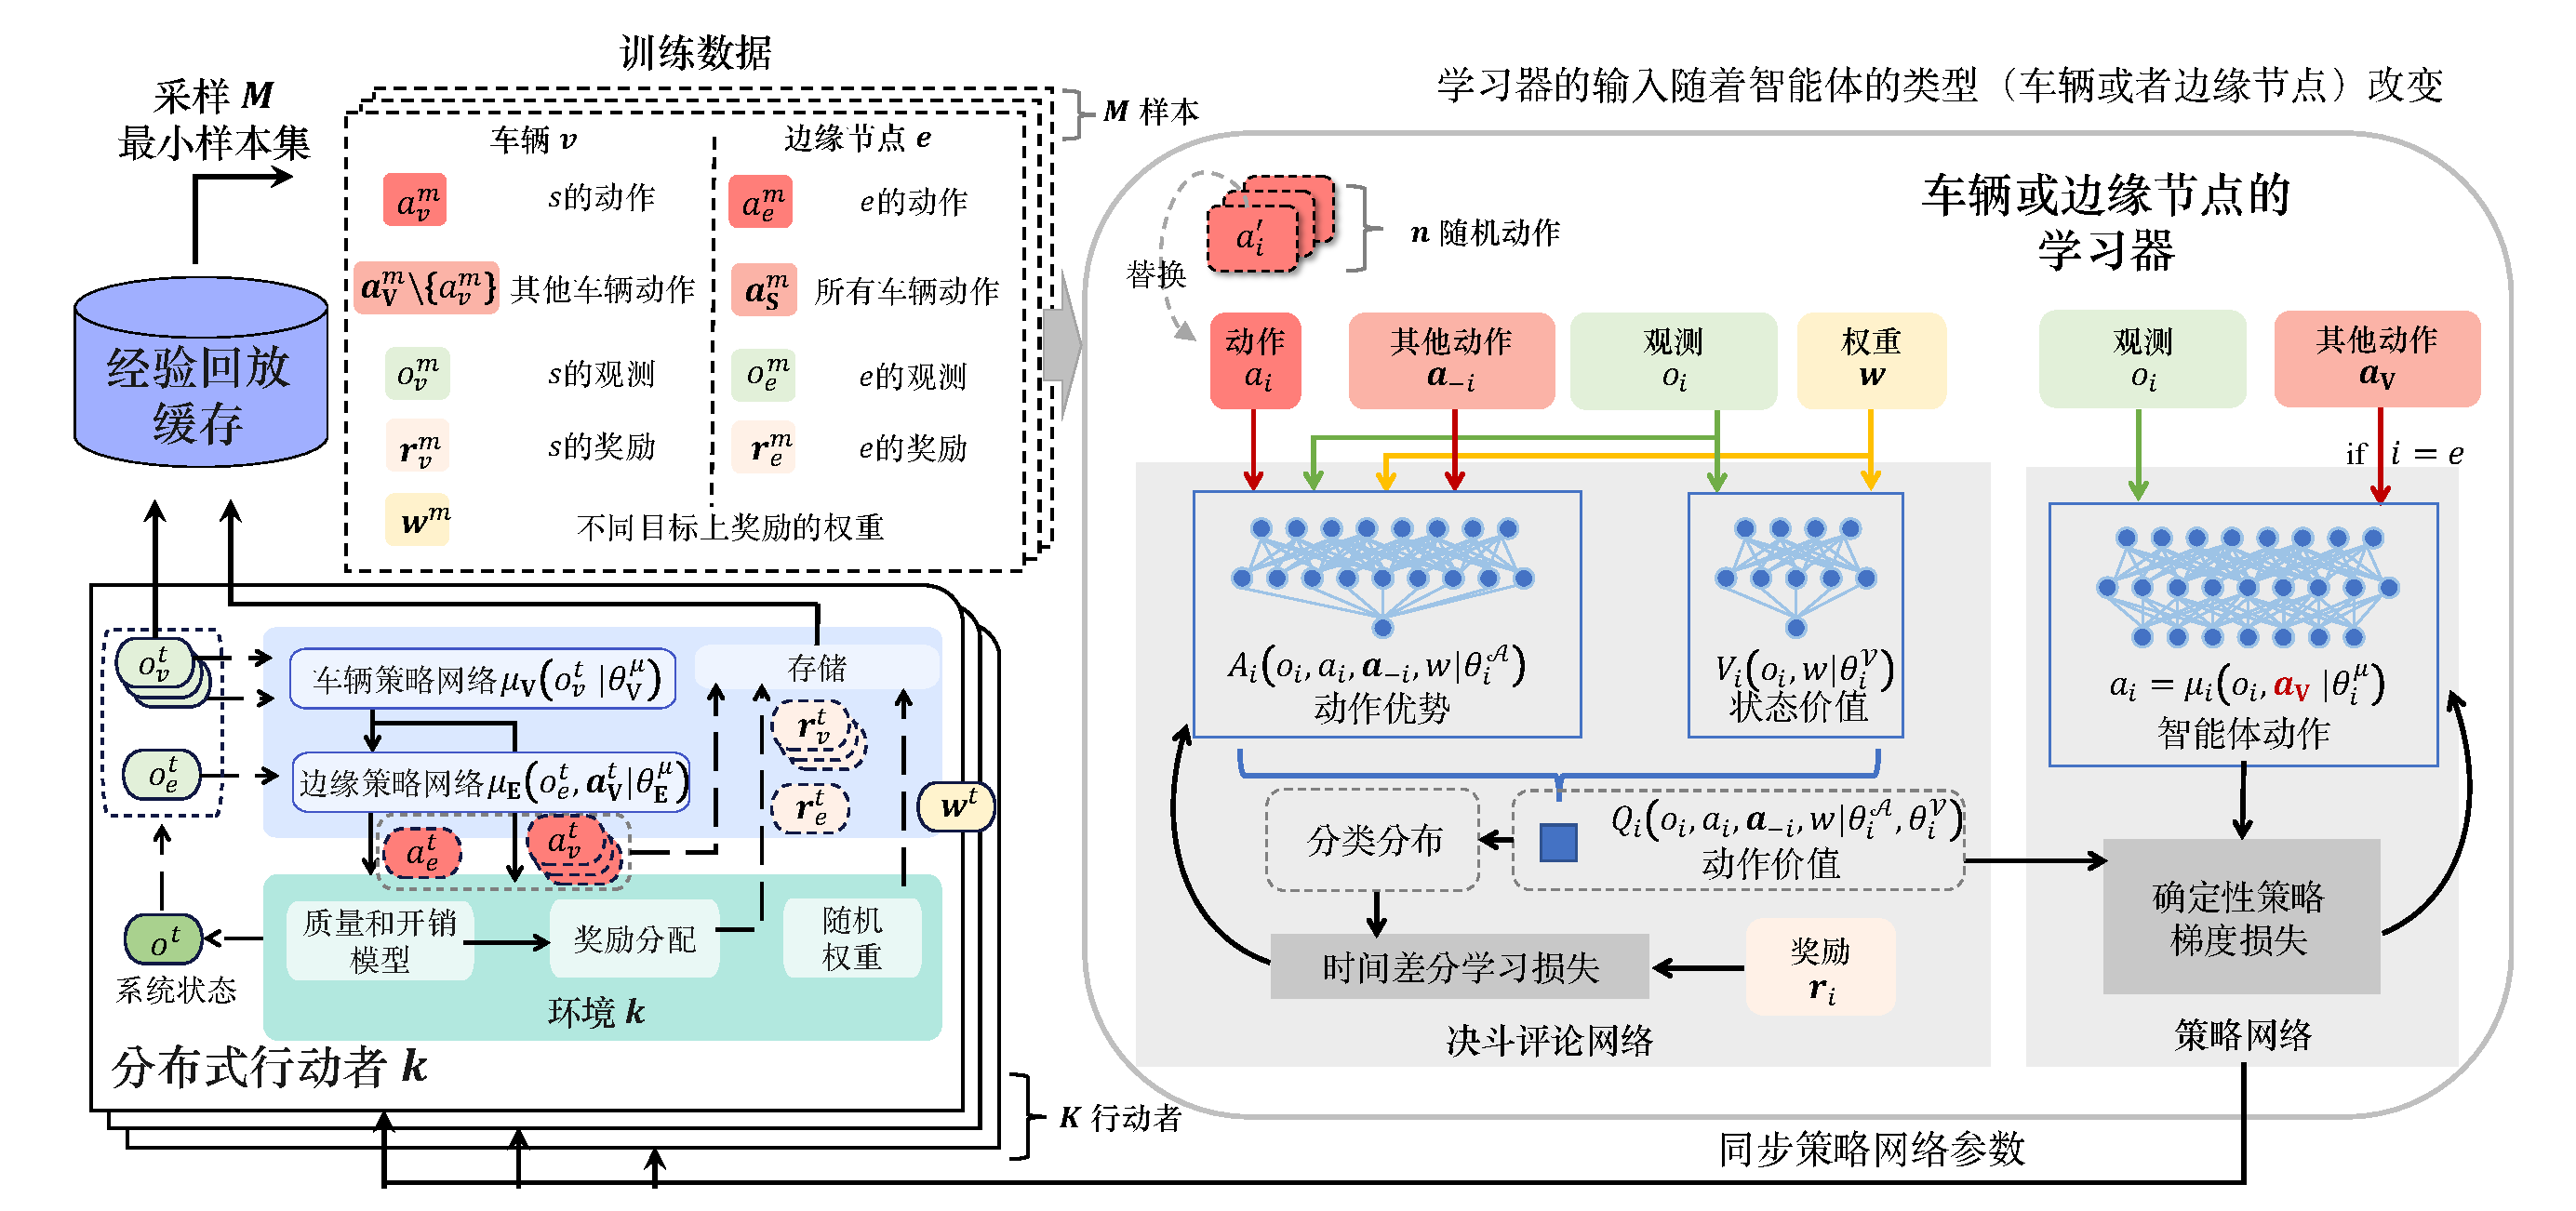
\includegraphics[width=1\columnwidth]{Fig4-2-solution-model.pdf}
  \bicaption{基于多目标的多智能体深度强化学习模型}{Multi-agent multi-objective deep reinforcement learning model}
  \label{fig 4-2}
\end{figure}


\SetKwInOut{KwIn}{输入}
\SetKwInOut{KwOut}{输出}

\begin{algorithm}[h]\small
\renewcommand{\algorithmcfname}{算法}
	\caption{基于多目标的多智能体深度强化学习}
	\KwIn{折扣因子 $\gamma$、批大小 $M$、回放经验缓存 $\mathcal{B}$、学习率$\alpha$和$\beta$、目标网络参数更新周期 $t_{\operatorname{tgt}}$、分布式行动者网络参数更新周期 $t_{\operatorname{act}}$、随机行动数量$N$}
	\KwOut{信息感知决策$\mathbf{C}_v^t$、信息感知频率决策$\lambda_{d, v}^{t}$、上传优先级决策$p_{d, v}^{t}$、传输功率$\pi_v^t$、V2I带宽分配$b_{v, e}^{t}$}
	初始化网络参数\\
	初始化经验回放缓存 $\mathcal{B}$\\
	启动 $K$ 分布式行动者并复制网络参数给行动者\\
	\For{\songti{迭代次数} $= 1$ \songti{到最大迭代次数}}{
		\For{\songti{时间片} $t = 1$ \songti{到} $T$}{
			从经验回放缓存$\mathcal{B}$随机采样$M$小批量\\
			通过目标评论家网络中DCN网络得到目标值\\
			基于分类分布的TD学习计算更新评论家网络\\
			更新本地策略和评论家网络\\
			\If{$t \mod t_{\operatorname{tgt}} = 0$}{
				更新目标网络\\
			}
			\If{$t \mod t_{\operatorname{act}} = 0$}{
				复制网络参数给分布式行动者\\
			}
		}
	}
\label{algorithm 4-1}
\end{algorithm}

\begin{algorithm}[t]\small
\renewcommand{\algorithmcfname}{算法}
	\caption{分布式行动者}
	\KwIn{车辆探索常数 $\epsilon_{v}$、边缘节点探索常数$\epsilon_{e}$、车辆本地观测 $\boldsymbol{o}_{v}^{t}$、边缘节点本地观测 $\boldsymbol{o}_{e}^{t}$}
	\KwOut{车辆动作$\boldsymbol{a}_{\mathbf{V}}^{t}$、边缘节点动作$\boldsymbol{a}_{e}^{t}$}
	\While{\songti{学习器没有结束}}{
		初始化一个随机过程 $\mathcal{N}$ 以进行探索\\
		生成随机权重 $\boldsymbol{w}^{t}$\\
		接收初始系统状态 $\boldsymbol{o}_{1}$\\
		\For{\songti{时间片} $t = 1$ \songti{到} $T$}{
			\For{\songti{车辆} $v=1$ \songti{到} $V$}{
				接收车辆本地观测 $\boldsymbol{o}_{v}^{t}$\\
				选择一个车辆动作 $\mu_{\mathbf{V}}\left(\boldsymbol{o}_{v}^{t} \mid \theta_{\mathbf{V}}^{\mu}\right)+\epsilon_{v} \mathcal{N}_{v}^{t}$\\
			}
			接收边缘节点本地观测 $\boldsymbol{o}_{e}^{t}$\\
			选择一个边缘节点动作 $\boldsymbol{a}_{e}^{t}=\mu_{\mathbf{E}}\left(\boldsymbol{o}_{e}^{t},  \boldsymbol{a}_{\boldsymbol{\mathbf{V}}}^{t} \mid \theta_{\mathbf{E}}^{\mu}\right)+\epsilon_{e} \mathcal{N}_{e}^{t}$\\
			接收奖励 $\boldsymbol{r}^{t}$ 和下一个系统状态 $\boldsymbol{o}^{t+1}$\\
			\For{\songti{车辆} $v=1$ \songti{到} $V$}{
				根据公式\ref{equ 4-40}计算车辆的差分奖励\\
			}
			根据公式\ref{equ 4-41}计算边缘节点的归一化奖励\\
			存储 $\left(\boldsymbol{o}^{t}, \boldsymbol{a}_{\mathbf{V}}^{t}, \boldsymbol{a}_{e}^{t}, \boldsymbol{r}_{\mathbf{V}}^{t}, \boldsymbol{r}_{e}^{t}, \boldsymbol{w}^{t}, \boldsymbol{o}^{t+1}\right)$ 到经验回放缓存 $\mathcal{B}$
		}
	}
\label{algorithm 4-2}
\end{algorithm}

\subsection{多智能体分布式策略执行}

在MAMO中,车辆和边缘节点分别通过本地策略网络分布式地决定动作。
车辆$v$在时间$t$上对系统状态的局部观测表示为:
	\begin{equation}
		\boldsymbol{o}_{v}^{t}=\left\{t, v, l_{v}^t, \mathbf{D}_{v}, \Phi_{v}, \mathbf{D}_{e}^{t}, \mathbf{D}_{\mathbf{I}_e^t}, \boldsymbol{w}^{t}\right\}
	\end{equation} 
\noindent 其中$t$为时间片索引;
$v$是车辆索引;$l_{v}^t$是车辆$v$的位置;
$\mathbf{D}_{v}$表示车辆$v$可以感知的信息集合;
$\Phi_{v}$代表$\mathbf{D}_{v}$中信息的感知开销;
$\mathbf{D}_{e}^{t}$ 代表$e$在时间$t$的边缘节点的缓存信息集;
$\mathbf{D}_{\mathbf{I}_e^t}$ 代表在时间$t$的边缘节点$e$中建模的视图所需的信息集合;
$\boldsymbol{w}^{t}$ 代表每个目标的权重向量,其在每次迭代中随机生成。
具体地,$\boldsymbol{w}^{t} = \begin{bmatrix}  w^{(1), t}  &  w^{(2), t} \end{bmatrix}$,其中$w^{(1), t} \in (0, 1)$和$w^{(2), t} \in (0, 1)$分别是VCPS质量和VCPS利润的权重,$\sum_{\forall i \in \{1, 2\}} w^{(j), t} = 1$。
另一方面,边缘节点$e$在时间$t$上对系统状态的局部观测表示为
\begin{equation}
	\boldsymbol{o}_{e}^{t}=\left\{t, e, \operatorname{\mathbf{Dis}}_{\mathbf{V}, e}^{t}, \mathbf{D}_{1}, \ldots, \mathbf{D}_{v}, \ldots, \mathbf{D}_{v}, \mathbf{D}_{e}^{t}, \mathbf{D}_{\mathbf{I}_e^t}, \boldsymbol{w}^{t} \right\}
\end{equation}
\noindent 其中$e$是边缘节点索引,$\operatorname{\mathbf{Dis}}_{\mathbf{V}, e}^{t}$代表车辆与边缘节点$e$之间的距离集合。
因此,系统在时间$t$的状态可以表示为$\boldsymbol{o}^{t}=\boldsymbol{o}_{e}^{t} \cup \boldsymbol{o}_{1}^{t} \cup \ldots \cup \boldsymbol{o}_{v}^{t} \cup \ldots \cup \boldsymbol{o}_{v}^{t}$。

车辆$v$的动作空间表示为:
\begin{equation}
	\boldsymbol{a}_{v}^{t} = \{ \mathbf{C}_v^t,  \{ \lambda_{d, v}^{t}, p_{d, v}^{t} \mid \forall d \in \mathbf{D}_{v}^t \} , \pi_v^t   \}
\end{equation}
其中,$\mathbf{C}_v^t$是感知决策;$\lambda_{d, v}^{t}$和$p_{d, v}^{t}$分别是信息$d$的感知频率和上传优先级,$\pi_v^t$是车辆$v$在时间$t$的传输功率。
车辆基于系统状态的本地观测,并通过本地车辆策略网络得到当前的动作。
\begin{equation}
	\boldsymbol{a}_{v}^{t}=\mu_{\mathbf{V}}\left(\boldsymbol{o}_{v}^{t} \mid \theta_{\mathbf{V}}^{\mu}\right)+\epsilon_{v} \mathcal{N}_{v}^{t}
\end{equation}
\noindent 其中,$\mathcal{N}_{v}^{t}$为探索噪音,以增加车辆动作的多样性,$\epsilon_{v}$为车辆$v$的探索常数。
车辆动作的集合被表示为 $\boldsymbol{a}_{\mathbf{V}}^{t} = \left\{\boldsymbol{a}_{v}^{t}\mid \forall v \in \mathbf{V}\right\}$。
另一方面,边缘节点$e$的动作空间表示为:
\begin{equation}
	\boldsymbol{a}_{e}^{t} = \{b_{v, e}^{t} \mid \forall v \in \mathbf{V}_{e}^{t}\}
\end{equation}
其中$b_{v, e}^t$是边缘节点$e$在时间$t$为车辆$v$分配的V2I带宽。
同样地,边缘节点$e$的动作可以由本地边缘策略网络根据系统状态以及车辆动作得到。
\begin{equation}
	\boldsymbol{a}_{e}^{t}=\mu_{\mathbf{E}}\left(\boldsymbol{o}_{e}^{t},  \boldsymbol{a}_{\boldsymbol{\mathbf{V}}}^{t} \mid \theta_{\mathbf{E}}^{\mu}\right)+\epsilon_{e} \mathcal{N}_{e}^{t}
\end{equation}
\noindent 其中$\mathcal{N}_{e}^{t}$和$\epsilon_{e}$分别为边缘节点$e$的探索噪声和探索常数。
此外,车辆和边缘节点的联合动作被表示为 $\boldsymbol{a}^{t}= \left\{\boldsymbol{a}_{e}^{t}, \boldsymbol{a}_{1}^{t}, \ldots, \boldsymbol{a}_{v}^{t}, \ldots, \boldsymbol{a}_{V}^{t}\right\}$。

环境通过执行联合动作获得系统奖励向量,其表示为:
	\begin{equation}
	\boldsymbol{r}^{t} = \begin{bmatrix}  r^{(1)}\left(\boldsymbol{a}_{\mathbf{V}}^{t},\boldsymbol{a}_{e}^{t} \mid \boldsymbol{o}^{t}\right)  &  r^{(2)}\left(\boldsymbol{a}_{\mathbf{V}}^{t},\boldsymbol{a}_{e}^{t} \mid \boldsymbol{o}^{t}\right) \end{bmatrix} ^{T}
	\end{equation}
	\noindent 其中 $r^{(1)}\left(\boldsymbol{a}_{\mathbf{V}}^{t},\boldsymbol{a}_{e}^{t} \mid \boldsymbol{o}^{t}\right)$ 和 $r^{(2)}\left(\boldsymbol{a}_{\mathbf{V}}^{t},\boldsymbol{a}_{e}^{t} \mid \boldsymbol{o}^{t}\right)$ 分别是两个目标(即实现的VCPS质量和VCPS 利润)的奖励,可以通过下式计算:  
	\begin{numcases}{}
			r^{(1)}\left(\boldsymbol{a}_{\mathbf{V}}^{t},\boldsymbol{a}_{e}^{t} \mid \boldsymbol{o}^{t}\right)=\frac{1}{\left|\mathbf{I}_e^t\right|} \sum_{\forall i \in \mathbf{I}_e^t}\operatorname{QV}_{i} \notag \\
			r^{(2)}\left(\boldsymbol{a}_{\mathbf{V}}^{t},\boldsymbol{a}_{e}^{t} \mid \boldsymbol{o}^{t}\right)=\frac{1}{\left|\mathbf{I}_e^t\right|} \sum_{\forall i \in \mathbf{I}_e^t} \operatorname{PV}_{j} 
	\end{numcases}
因此,车辆$v$在第$i$个目标中的奖励可以通过基于差分奖励的信用分配方案 \cite{foerster2018counterfactual} 得到,其为系统奖励和没有其行动所取得的奖励之间的差值,其表示为:
\begin{equation}
r_{v}^{(j), t}=r^{(j)}\left(\boldsymbol{a}_{\mathbf{V}}^{t},\boldsymbol{a}_{e}^{t} \mid \boldsymbol{o}^{t}\right)-r^{(j)}\left(\boldsymbol{a}_{\mathbf{V}-s}^{t},\boldsymbol{a}_{e}^{t} \mid \boldsymbol{o}^{t}\right), \forall i \in \{1, 2\}
\label{equ 4-40}
\end{equation}
\noindent 其中 $r^{(j)}\left(\boldsymbol{a}_{\mathbf{V}-s}^{t},\boldsymbol{a}_{e}^{t} \mid \boldsymbol{o}^{t}\right)$ 是在没有车辆$v$贡献的情况下实现的系统奖励,它可以通过设置车辆$v$的空动作集得到。
车辆$v$在时间$t$的奖励向量表示为$\boldsymbol{r}_{v}^{t} = \begin{bmatrix}  r_{v}^{(1), t}  &  r_{v}^{(2), t} \end{bmatrix} ^{T}$。
车辆的差分奖励集合表示为 $\boldsymbol{r}_{\mathbf{V}}^{t}=\{ \boldsymbol{r}_{v}^{t} \mid \forall v \in \mathbf{V}\}$。

另一方面,系统奖励通过最小-最大归一化进一步转化为边缘节点的归一化奖励。
边缘节点$e$在时间$t$的第$i$个目标中的奖励由以下方式计算:
\begin{equation}
	r_{e}^{(j), t}= \frac{r^{(j)}\left(\boldsymbol{a}_{\mathbf{V}}^{t},\boldsymbol{a}_{e}^{t} \mid \boldsymbol{o}^{t}\right) - \min \limits_{\forall {\boldsymbol{a}_{e}^{t}}^{\prime}} r^{(j)}\left(\boldsymbol{a}_{\mathbf{V}}^{t}, {\boldsymbol{a}_{e}^{t}}^{\prime} \mid \boldsymbol{o}^{t}\right)} {\max \limits_{\forall {\boldsymbol{a}_{e}^{t}}^{\prime}} r^{(j)}\left(\boldsymbol{a}_{\mathbf{V}}^{t}, {\boldsymbol{a}_{e}^{t}}^{\prime} \mid \boldsymbol{o}^{t}\right) - \min \limits_{\forall {\boldsymbol{a}_{e}^{t}}^{\prime}} r^{(j)}\left(\boldsymbol{a}_{\mathbf{V}}^{t}, {\boldsymbol{a}_{e}^{t}}^{\prime} \mid \boldsymbol{o}^{t}\right)}
\label{equ 4-41}
\end{equation}
\noindent 其中 $\min \limits_{\forall {\boldsymbol{a}_{e}^{t}}^{\prime}} r^{(j)} (\boldsymbol{a}_{\mathbf{V}}^{t}, {\boldsymbol{a}_{e}^{t}}^{\prime} \mid \boldsymbol{o}^{t})$ 和 $\max \limits_{\forall {\boldsymbol{a}_{e}^{t}}^{\prime}} r^{(j)}(\boldsymbol{a}_{\mathbf{V}}^{t}, {\boldsymbol{a}_{e}^{t}}^{\prime} \mid \boldsymbol{o}^{t})$ 分别是在相同的系统状态$\boldsymbol{o}^{t}$下,车辆动作$\boldsymbol{a}_{\mathbf{V}}^{t}$不变时,可实现的系统奖励最小值和最大值。
边缘节点$e$在时间$t$的奖励向量表示为 $\boldsymbol{r}_{e}^{t} = \begin{bmatrix}  r_{e}^{(1), t}  &  r_{e}^{(2), t} \end{bmatrix} ^{T}$。
交互经验包括当前系统状态$\boldsymbol{o}^{t}$、车辆动作$\boldsymbol{a}_{\mathbf{V}}^{t}$、边缘节点动作$\boldsymbol{a}_{e}^{t}$、车辆奖励$\boldsymbol{r}_{\mathbf{V}}^{t}$、边缘节点奖励$\boldsymbol{r}_{e}^{t}$、权重$\boldsymbol{w}^{t}$,以及下一时刻系统状态$\boldsymbol{o}^{t+1}$都存储到经验回放缓存$\mathcal{B}$。

\subsection{多目标策略评估}

本章节阐述了针对多目标的策略评估,具体地,提出了决斗评论家网络,根据状态的价值和行动的优势来评估智能体的行动。
在DCN中有两个全连接的网络,即动作优势网络和状态价值网络。
车辆和边缘节点的AA网络参数分别表示为 $\theta_{\mathbf{V}}^{\mathscr{A}}$ 和 $\theta_{\mathbf{E}}^{\mathscr{A}}$。
同样,车辆和边缘节点的SV网络的参数分别表示为 $\theta_{\mathbf{V}}^{\mathscr{V}}$ 和 $\theta_{\mathbf{E}}^{\mathscr{V}}$。
用$A_{\mathbf{V}}\left({o}_{v}^{m},  {a}_{v}^{m}, \boldsymbol{a}_{\boldsymbol{\mathbf{V}}-v}^{m}, \boldsymbol{w}^{m} \mid \theta_{\mathbf{V}}^{\mathscr{A}} \right)$表示车辆$v$中AA网络的输出标量, 其中 $\boldsymbol{a}_{\boldsymbol{\mathbf{V}}-v}^{m}$ 表示其他车辆动作。
同样地,以边缘节点$e$为输入的AA网络的输出标量表示为 $A_{\mathbf{E}}\left({o}_{e}^{m},  {a}_{e}^{m}, \boldsymbol{a}_{\boldsymbol{\mathbf{V}}}^{m}, \boldsymbol{w}^{m} \mid \theta_{\mathbf{E}}^{\mathscr{A}} \right)$, 其中 $\boldsymbol{a}_{\boldsymbol{\mathbf{V}}}^{m}$ 表示所有车辆动作。
车辆$v$的SV网络的输出标量表示为 $V_{\mathbf{V}}\left({o}_{v}^{m}, \boldsymbol{w}^{m} \mid \theta_{\mathbf{V}}^{\mathscr{V}} \right)$。
同样地,边缘节点$e$的SV网络的输出标量表示为 $V_{\mathbf{E}}\left({o}_{e}^{m}, \boldsymbol{w}^{m} \mid \theta_{\mathbf{E}}^{\mathscr{V}} \right)$。

多目标策略评估由三个步骤组成。
首先,AA网络基于观测、动作和权重输出智能体动作的优势。
其次,VS网络根据观测和权重,输出当前状态的价值。
最后,采用一个聚合模块,根据行动优势和状态价值,输出智能体动作的价值。
具体来说,在AA网络中随机生成$N$个动作并将智能体动作替换,以评估当前动作对于随机行动的平均优势。
用${a}_{v}^{m, n}$和${a}_{e}^{m, n}$分别表示车辆$v$和边缘节点$e$的第$n$个随机动作。
因此,车辆$v$和边缘节点$e$的第$n$个随机动作的优势可分别表示为 $A_{\mathbf{V}}\left({o}_{v}^{m},  {a}_{v}^{m, n}, \boldsymbol{a}_{\boldsymbol{\mathbf{V}}-v}^{m}, \boldsymbol{w}^{m} \mid \theta_{v}^{\mathscr{A}} \right)$ 和 $A_{\mathbf{E}}\left({o}_{e}^{m},  {a}_{e}^{m, n}, \boldsymbol{a}_{\boldsymbol{\mathbf{V}}}^{m}, \boldsymbol{w}^{m} \mid \theta_{\mathbf{E}}^{\mathscr{A}} \right)$。

进一步,通过评估智能体动作相对于随机动作的平均优势,对价值函数进行聚合。
因此,车辆$v\in\mathbf{V}$和边缘节点$e$的动作价值是通过下式计算: 
\begin{align}
    Q_{\mathbf{V}}\left({o}_{v}^{m}, {a}_{v}^{m}, \boldsymbol{a}_{\boldsymbol{\mathbf{V}}-v}^{m}, \boldsymbol{w}^{m} \mid \theta_{\mathbf{V}}^{Q} \right) &= V_{\mathbf{V}}\left({o}_{v}^{m}, \boldsymbol{w}^{m} \mid \theta_{\mathbf{V}}^{\mathscr{V}} \right) + A_{\mathbf{V}}\left({o}_{v}^{m},  {a}_{v}^{m}, \boldsymbol{a}_{\boldsymbol{\mathbf{V}}-v}^{m}, \boldsymbol{w}^{m} \mid \theta_{\mathbf{V}}^{\mathscr{A}} \right) \notag \\
    &- \frac{1}{N} \sum_{\forall n} A_{\mathbf{V}}\left({o}_{v}^{m},  {a}_{v}^{m, n}, \boldsymbol{a}_{\boldsymbol{\mathbf{V}}-v}^{m}, \boldsymbol{w}^{m} \mid \theta_{\mathbf{V}}^{\mathscr{A}} \right)
\end{align}
\begin{align}
    Q_{E}\left({o}_{e}^{m},  {a}_{e}^{m}, \boldsymbol{a}_{\boldsymbol{\mathbf{V}}}^{m}, \boldsymbol{w}^{m} \mid \theta_{\mathbf{E}}^{Q} \right) &= V_{\mathbf{E}}\left({o}_{e}^{m}, \boldsymbol{w}^{m} \mid \theta_{\mathbf{E}}^{\mathscr{V}} \right) + A_{\mathbf{E}}\left({o}_{e}^{m},  {a}_{e}^{m}, \boldsymbol{a}_{\boldsymbol{\mathbf{V}}}^{m}, \boldsymbol{w}^{m} \mid \theta_{\mathbf{E}}^{\mathscr{A}} \right) \notag \\
    &- \frac{1}{N} \sum_{\forall n} A_{\mathbf{E}}\left({o}_{e}^{m},  {a}_{e}^{m, n}, \boldsymbol{a}_{\boldsymbol{\mathbf{V}}}^{m}, \boldsymbol{w}^{m} \mid \theta_{\mathbf{E}}^{\mathscr{A}} \right)
\end{align}
其中,$\theta_{\mathbf{V}}^{Q}$ 和 $\theta_{\mathbf{V}}^{Q}$ 包含相应的AA和SV网络的参数。
\begin{align}
	\theta_{\mathbf{V}}^{Q} = (\theta_{\mathbf{V}}^{\mathscr{A}}, \theta_{\mathbf{V}}^{\mathscr{V}}), \theta_{\mathbf{V}}^{Q^{\prime}} = (\theta_{\mathbf{V}}^{\mathscr{A}^{\prime}}, \theta_{\mathbf{V}}^{\mathscr{V}^{\prime}}) \\
	\theta_{\mathbf{E}}^{Q} = (\theta_{\mathbf{E}}^{\mathscr{A}}, \theta_{\mathbf{E}}^{\mathscr{V}}), \theta_{\mathbf{E}}^{Q^{\prime}} = (\theta_{\mathbf{E}}^{\mathscr{A}^{\prime}}, \theta_{\mathbf{E}}^{\mathscr{V}^{\prime}})
\end{align}

\subsection{网络学习和更新}

从经验回放缓存$\mathcal{B}$中抽出$M$小批量,以训练车辆和边缘节点的策略和评论家网络,其中单个样本表示为 $\left(\boldsymbol{o}_{\mathbf{V}}^{m}, {o}_{e}^{m}, \boldsymbol{w}^{m}, \boldsymbol{a}_{\mathbf{V}}^{m}, {a}_{e}^{m}, \boldsymbol{r}_{\mathbf{V}}^{m}, \boldsymbol{r}_{e}^{m}, \boldsymbol{o}_{\mathbf{V}}^{m+1}, {o}_{e}^{m+1}, \boldsymbol{w}^{m+1}\right)$。
车辆$v$的目标值表示为:
\begin{equation}
	y_{v}^{m} = \boldsymbol{r}_{v}^{m} \boldsymbol{w}^{m} +\gamma Q_{\mathbf{V}}^{\prime}\left({o}_{v}^{m+1},  {a}_{v}^{m+1}, \boldsymbol{a}_{\boldsymbol{\mathbf{V}}-v}^{m+1}, \boldsymbol{w}^{m+1} \mid \theta_{\mathbf{V}}^{Q^{\prime}} \right)
\end{equation}
\noindent 其中 $Q_{\mathbf{V}}^{\prime}({o}_{v}^{m+1},  {a}_{v}^{m+1}, \boldsymbol{a}_{\boldsymbol{\mathbf{V}}-v}^{m+1}, \boldsymbol{w}^{m+1} \mid \theta_{\mathbf{V}}^{Q^{\prime}})$ 是目标车辆评论家网络产生的动作价值。
$\gamma$是折扣因子。
$\boldsymbol{a}_{\boldsymbol{\mathbf{V}}-v}^{m+1}$ 是没有车辆$v$的下一时刻车辆动作。
\begin{equation}
	\boldsymbol{a}_{\boldsymbol{\mathbf{V}}-v}^{m+1} = \{ {a}_{1}^{m+1}, \ldots, {a}_{s-1}^{m+1}, {a}_{s+1}^{m+1}, \ldots, {a}_{v}^{m+1} \}
\end{equation}
而 ${a}_{v}^{m+1}$ 是目标车辆策略网络根据对下一时刻系统状态的局部观测产生的车辆$v$的下一时刻动作。
\begin{equation}
	{a}_{v}^{m+1} = \mu_{\mathbf{V}}^{\prime}(\boldsymbol{o}_{v}^{m+1} \mid \theta_{\mathbf{V}}^{\mu^{\prime}})
\end{equation}
类似地,边缘节点$e$的目标值表示为:
\begin{equation}
	y_{e}^{m} = \boldsymbol{r}_{e}^{m} \boldsymbol{w}^{m} +\gamma Q_{\mathbf{E}}^{\prime}\left({o}_{e}^{m+1},  {a}_{e}^{m+1}, \boldsymbol{a}_{\boldsymbol{\mathbf{V}}}^{m+1}, \boldsymbol{w}^{m+1} \mid \theta_{\mathbf{E}}^{Q^{\prime}} \right)
\end{equation}
\noindent 其中 $Q_{\mathbf{E}}^{\prime}({o}_{e}^{m+1},  {a}_{e}^{m+1}, \boldsymbol{a}_{\boldsymbol{\mathbf{V}}}^{m+1}, \boldsymbol{w}^{m+1} \mid \theta_{\mathbf{E}}^{Q^{\prime}})$ 表示由目标边缘评论家网络产生的动作价值。
$\boldsymbol{a}_{\boldsymbol{\mathbf{V}}}^{m+1}$ 是下一时刻车辆动作。
${a}_{e}^{m+1}$表示下一时刻边缘节点动作,该动作可由目标边缘策略网络根据其对下一时刻系统状态的局部观测获得,即${a}_{e}^{m+1} = \mu_{\mathbf{E}}^{\prime}(\boldsymbol{o}_{e}^{m+1}, \boldsymbol{a}_{\mathbf{V}}^{m+1} \mid \theta_{\mathbf{E}}^{\mu^{\prime}})$。

车辆评论家网络和边缘评论家网络的损失函数是通过分类分布的时间差分(Temporal Difference, TD)学习得到的,其表示为:
\begin{equation}
	\mathcal{L}\left(\theta_{\mathbf{V}}^{Q}\right)=\frac{1}{M} \sum_{m} \frac{1}{S} \sum_{v} {Y_v^{m}}
\end{equation}
\begin{equation}
	\mathcal{L}\left(\theta_{\mathbf{E}}^{Q}\right)=\frac{1}{M} \sum_{m} {Y_e^{m}}
\end{equation}
\noindent 其中$Y_v^{m}$和$Y_e^{m}$分别是车辆$v$和边缘节点$e$的目标值和局部评论家网络产生的动作价值之差的平方。
\begin{equation}
	\begin{aligned}
		Y_v^{m} &= \left(y_{v}^{m}-Q_{\mathbf{V}}\left({o}_{v}^{m},  {a}_{v}^{m}, \boldsymbol{a}_{\boldsymbol{\mathbf{V}}-v}^{m}, \boldsymbol{w}^{m} \mid \theta_{\mathbf{V}}^{Q} \right)\right)^{2} \\
	\end{aligned}
\end{equation}
\begin{equation}
	\begin{aligned}
		Y_e^{m} &=\left(y_{e}^{m}-Q_{\mathbf{E}}\left({o}_{e}^{m},  {a}_{e}^{m}, \boldsymbol{a}_{\boldsymbol{\mathbf{V}}}^{m}, \boldsymbol{w}^{m} \mid \theta_{\mathbf{V}}^{Q} \right)\right)^{2} \\
	\end{aligned}
\end{equation}
车辆和边缘策略网络参数通过确定性的策略梯度进行更新。
\begin{equation}
	\nabla_{\theta_{\mathbf{V}}^{\mu}} \mathcal{J} (\theta_{\mathbf{V}}^{\mu}) \approx \frac{1}{M} \sum_{m} \frac{1}{S} \sum_{v} P_{v}^{m} 
\end{equation}
\begin{equation}
	\nabla_{\theta_{\mathbf{E}}^{\mu}} \mathcal{J} (\theta_{\mathbf{E}}^{\mu}) \approx \frac{1}{M} \sum_{m} P_{e}^{m} 
\end{equation}
\noindent 其中 
\begin{equation}
P_{v}^{m} = \nabla_{{a}_{v}^{m}} Q_{\mathbf{V}}\left({o}_{v}^{m}, {a}_{v}^{m}, \boldsymbol{a}_{\boldsymbol{\mathbf{V}}-v}^{m}, \boldsymbol{w}^{m} \mid \theta_{v}^{Q} \right) \nabla_{\theta_{\mathbf{V}}^{\mu}} \mu_{\mathbf{V}}\left({o}_{v}^{m} \mid \theta_{\mathbf{V}}^{\mu}\right)
\end{equation}
\begin{equation}
P_{e}^{m} = \nabla_{{a}_{e}^{m}} Q_{\mathbf{E}}\left({o}_{e}^{m}, {a}_{e}^{m}, \boldsymbol{a}_{\boldsymbol{\mathbf{V}}}^{m}, \boldsymbol{w}^{m} \mid \theta_{\mathbf{E}}^{Q} \right) \nabla_{\theta_{\mathbf{E}}^{\mu}} \mu_{\mathbf{E}}\left({o}_{e}^{m}, {\boldsymbol{a}}_{\boldsymbol{\mathbf{V}}}^{m} \mid \theta_{\mathbf{E}}^{\mu}\right)
\end{equation}

本地策略和评论家网络参数分别以$\alpha$和$\beta$的学习率更新。
特别地,车辆和边缘节点定期更新目标网络的参数,即当$t \mod t_{\operatorname{tgt}} = 0$, 其中 $t_{\operatorname{tgt}}$ 是目标网络的参数更新周期。
\begin{align}
	\theta_{\mathbf{V}}^{\mu^{\prime}} \leftarrow n_{\mathbf{V}} \theta_{\mathbf{V}}^{\mu}+(1-n_{\mathbf{V}}) \theta_{\mathbf{V}}^{\mu^{\prime}}, \theta_{\mathbf{V}}^{Q^{\prime}} \leftarrow n_{\mathbf{V}} \theta_{\mathbf{V}}^{Q}+(1-n_{\mathbf{V}}) \theta_{\mathbf{V}}^{Q^{\prime}}\\
	\theta_{\mathbf{E}}^{\mu^{\prime}} \leftarrow n_{\mathbf{E}} \theta_{\mathbf{E}}^{\mu}+(1-n_{\mathbf{E}}) \theta_{\mathbf{E}}^{\mu^{\prime}}, \theta_{\mathbf{E}}^{Q^{\prime}} \leftarrow n_{\mathbf{E}} \theta_{\mathbf{E}}^{Q}+(1-n_{\mathbf{E}})  \theta_{\mathbf{E}}^{Q^{\prime}}
\end{align}
\noindent 其中 $n_{\mathbf{V}} \ll 1$ 和 $n_{\mathbf{E}} \ll 1$。
同样,分布式行动者的策略网络参数也会定期更新,即当$t \mod t_{\operatorname{act}} = 0$,其中 $t_{\operatorname{act}}$ 是分布式行动者的策略网络的参数更新周期。
\begin{align}
	\theta_{\mathbf{V}, k}^{\mu} \leftarrow \theta^{{\mu}^{\prime}}_{\mathbf{V}}, \theta_{\mathbf{V}, k}^{Q} \leftarrow \theta_{\mathbf{V}}^{Q^{\prime}}, \forall k \in \{1, 2, \ldots, K\}\\
	\theta_{\mathbf{E}, k}^{\mu} \leftarrow \theta_{\mathbf{E}}^{\mu^{\prime}}, \theta_{\mathbf{E}, k}^{Q} \leftarrow \theta_{\mathbf{E}}^{Q^{\prime}}, \forall k \in \{1, 2, \ldots, K\}
\end{align}

\section{实验结果与分析}\label{section 4-6}

\subsection{实验设置}

本章节使用Python 3.9.13和TensorFlow 2.8.0来搭建仿真实验模型以评估所提MAMO方案的性能,其运行在配备AMD Ryzen 9 5950X 16核处理器@ 3.4 GHz,两个NVIDIA GeForce RTX 3090 GPU和64 GB内存的Ubuntu 20.04服务器上。
在参考\inlinecite{sadek2009distributed}和\inlinecite{wang2019delay}的基础上,实验仿真参数设置如下:
V2I通信范围被设定为500 m。
传输功率被设定为100 mW。
AWGN和可靠性阈值分别设置为-90 dBm和0.9。
V2I通信的信道衰减增益遵循高斯分布,其均值为2,方差为0.4。
$\hat{\Theta_{i}}$、$\hat{\Psi_{i}}$、$\hat{\Xi_{i}}$、$\hat{\Phi_{i}}$和$\hat{\Omega_{i}}$的加权系数分别设置为0.6、0.4、0.2、0.4和0.4。

MAMO中策略和评论家网络的架构和超参数描述如下:
本地策略网络是一个有两个隐藏层的四层全连接神经网络,其中神经元的数量分别为256和128。
目标策略网络的结构与本地策略网络相同。
本地评论家网络是一个四层全连接神经网络,有两个隐藏层,其中神经元的数量分别为512和256。
目标评论家网络的结构与本地评论家网络相同。
折扣率、批大小和最大经验回放缓存大小分别为0.996、256和1$\times10^{6}$。
策略网络和评论家网络的学习率分别为1$\times10^{-4}$和1$\times10^{-4}$。

进一步,本章节实现了三个比较算法,其具体细节介绍如下:
\begin{itemize}
	\item \textbf{随机分配}: 随机选择一个动作来确定感知信息、感知频率、上传优先级、传输功率和V2I带宽分配。
	\item \textbf{分布式深度确定性策略梯度}\cite{barth2018distributed}: 在边缘节点实现了一个智能体,根据系统状态,集中式地确定感知信息、感知频率、上传优先级、传输功率和V2I带宽分配。VCPS质量和VCPS 利润权重分别设定为0.5和0.5。
	\item \textbf{多智能体分布式深度确定性策略梯度}: 其为D4PG的多智能体版本,并在车辆上分布式实现,根据对物理环境的局部观测决定感知信息、感知频率、上传优先级和传输功率,边缘节点决定V2I带宽分配。VCPS质量和VCPS 利润权重分别设为0.5和0.5。
\end{itemize}

为了评估算法在视图建模质量和有效性方面的表现,本章设计了以下两个新的指标。
\begin{itemize}
	\item \textbf{单位开销质量}:其定义为花费单位开销实现的VCPS质量,其计算公式为:
		\begin{equation}
			\operatorname{QPUC}=\frac{\sum_{\forall t \in \mathbf{T}} \sum_{\forall e \in \mathbf{E}} \sum_{\forall i \in \mathbf{I}_e^t} \mathrm{QV}_i}{\sum_{\forall t \in \mathbf{T}} \sum_{\forall e \in \mathbf{E}} \sum_{\forall i \in \mathbf{I}_e^t} \mathrm{CV}_i}
		\end{equation}
		其中$\mathrm{QV}_i$和$\mathrm{CV}_i$分别是视图$i$的质量和开销。
	\item \textbf{单位质量利润}:其定义为单位VCPS质量所实现的VCPS 利润,其计算公式为:
		\begin{equation}
		\operatorname{PPUQ}=\frac{\sum_{\forall t \in \mathbf{T}} \sum_{\forall e \in \mathbf{E}} \sum_{\forall i \in \mathbf{I}_e^t}\mathrm{PV}_i}{\sum_{\forall t \in \mathbf{T}} \sum_{\forall e \in \mathbf{E}} \sum_{\forall i \in \mathbf{I}_e^t} \mathrm{QV}_i}
		\end{equation}
		其中$\mathrm{PV}_i$和$\mathrm{CV}_i$分别是视图$i$的利润和开销。
\end{itemize}
QPUC越高表明它能在相同的开销下实现更高的VCPS质量,而PPUQ越高表明它能更有效地使用感知和通信资源。上述指标全面显示了算法在同时最大化VCPS质量和最小化VCPS 开销的性能。
本章进一步基于公式\ref{equ 4-16}、\ref{equ 4-20}、\ref{equ 4-21}和\ref{equ 4-23}设计了四个指标,分别是\textbf{平均及时性}(Average Timeliness, AT)、\textbf{平均冗余度}(Average Redundancy, AR)、\textbf{平均感知开销}(Average Sensing Cost, ASC)和\textbf{平均传输开销}(Average Transmission Cost, ATC)。 

\subsection{实验结果与分析}

\textbf{1) 算法收敛性:}图\ref{fig 4-3}比较了四种算法的收敛性。其中,图\ref{fig 4-3}(a)和\ref{fig 4-3}(b)分别展示了四种算法的QPUC和PPUQ表现。X轴表示迭代次数,Y轴表示达到的QPUC和PPUQ。QPUC和PPUQ越高,表明算法在VCPS质量和VCPS开销方面表现越好。MAMO在大约850次迭代后,达到了最高的QPUC(约13.6)和最高的PPUQ(约1.13)。相比之下,RA、D4PG和MAD4PG分别实现了约2.29、7.34和2.58的QPUC,并分别实现了约0.87、0.99和0.81的PPUQ。与RA、D4PG和MAD4PG相比,MAMO在QPUC方面分别实现了约494.1\%、85.5\%和428.8\%的提升,在PPUQ方面分别实现了约30.6\%、14.2\%和40.7\%的改善。值得注意的是,MAMO是唯一一个能够同时改善QPUC和PPUQ的方案。这显示了MAMO在同时实现QPUC和PPUQ最大化方面的优势。

\begin{figure}[h]
 \centering
 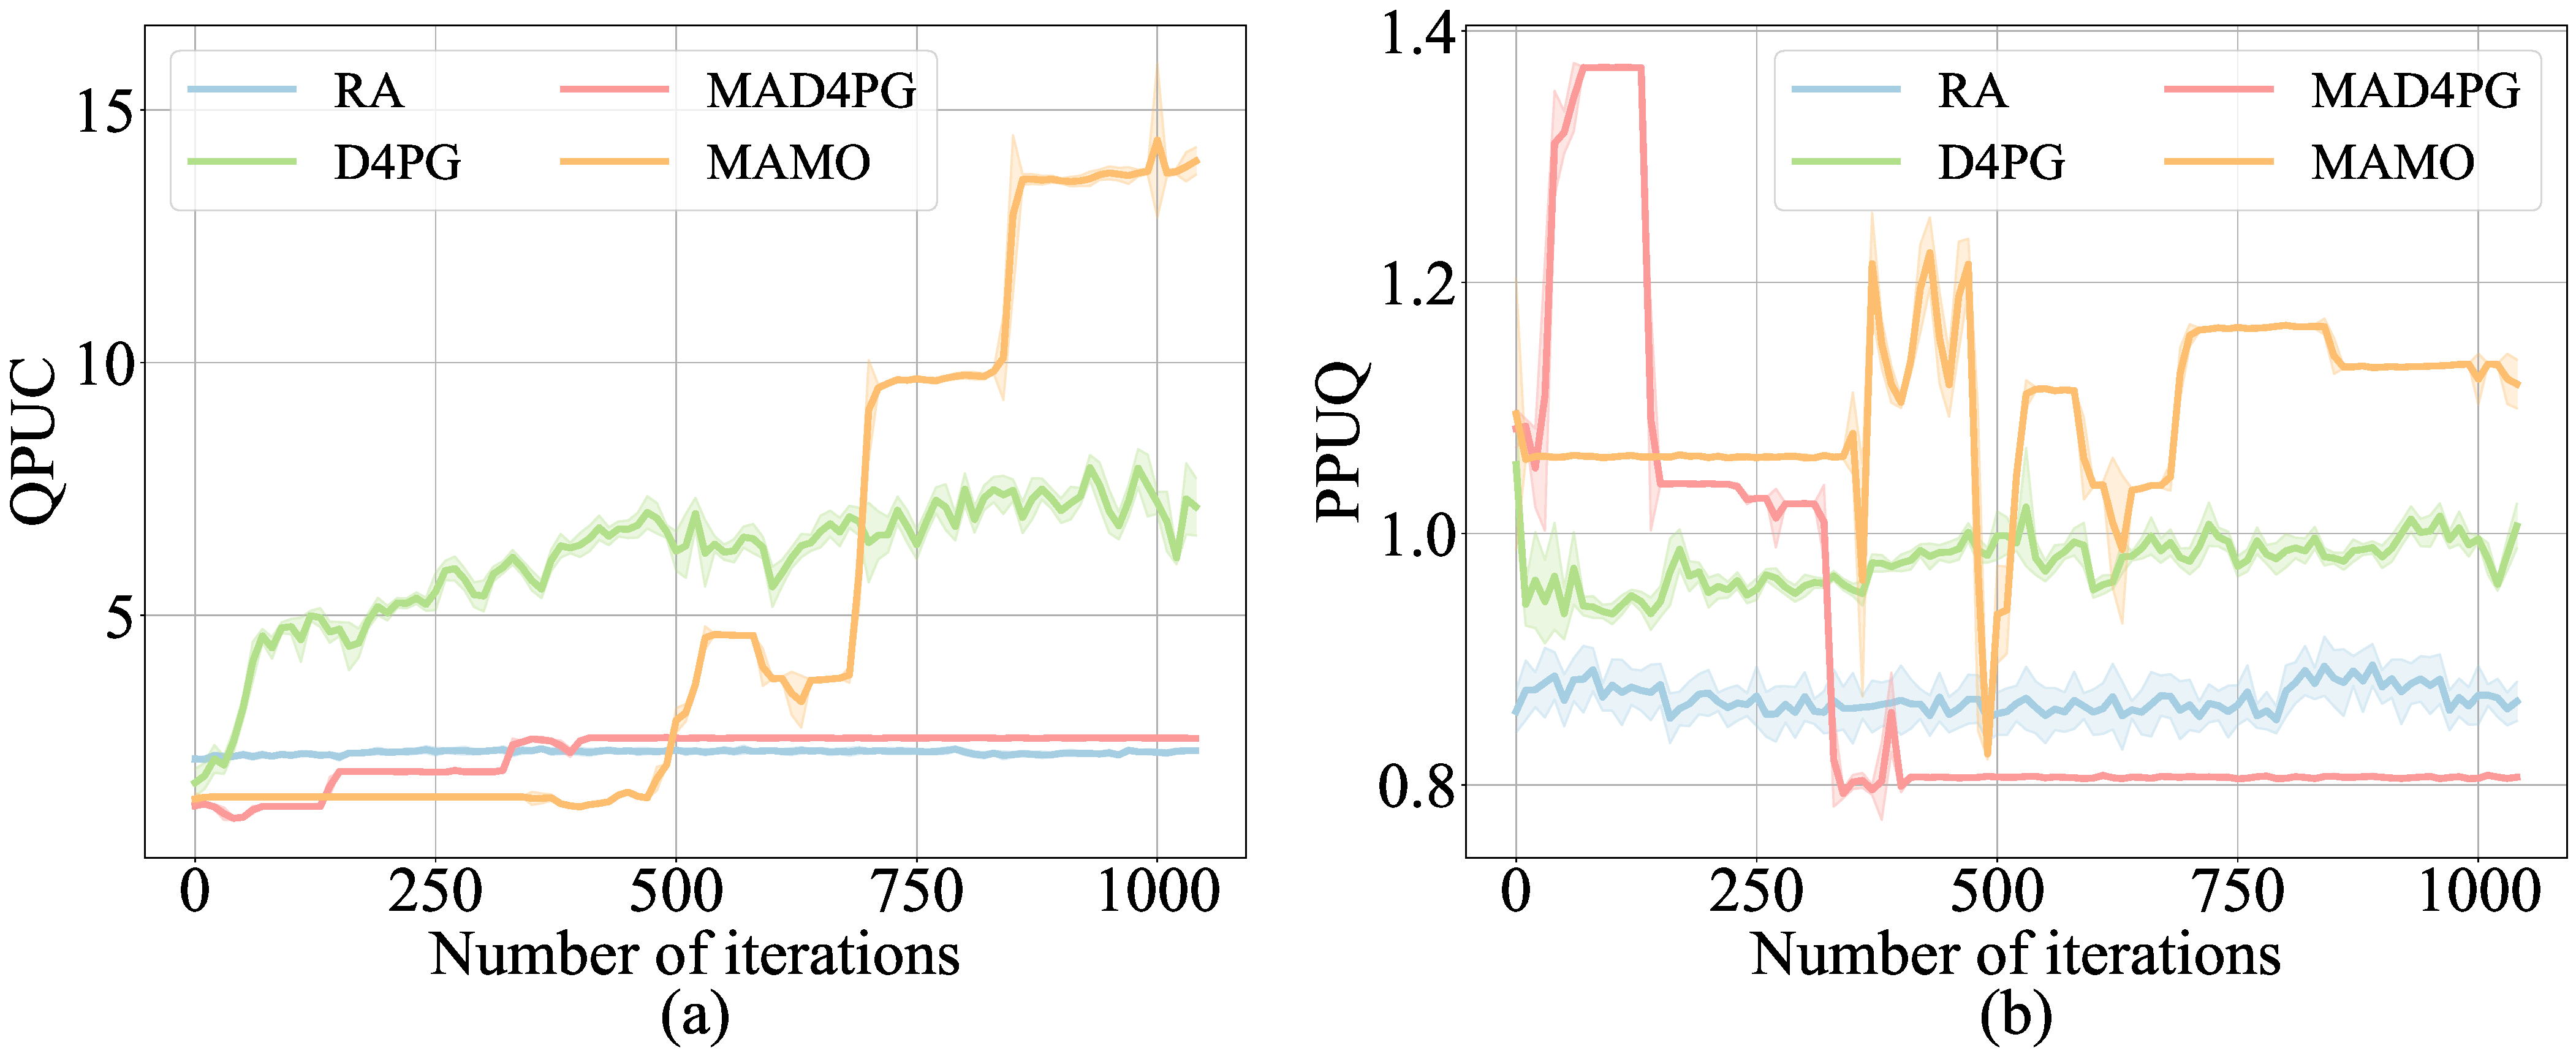
\includegraphics[width=1\columnwidth]{Fig4-3-different-algorithms.pdf}
 \bicaption[算法收敛性比较]{算法收敛性比较,其显示与RA、D4PG和MAD4PG相比,MAMO在收敛后(约850次迭代)达到了最高的QPUC和最高的PPUQ。(a)单位开销质量(b)单位质量利润}[Convergence comparison]{Convergence comparison, which shows MAMO achieves the highest QPUC and the highest PPUQ compared with RA, D4PG, and MAD4PG after convergence (around 850 iterations). (a) Quality per unit cost (b) Profit per unit quality}
 \label{fig 4-3}
\end{figure}

\begin{figure}[h]
 \centering
 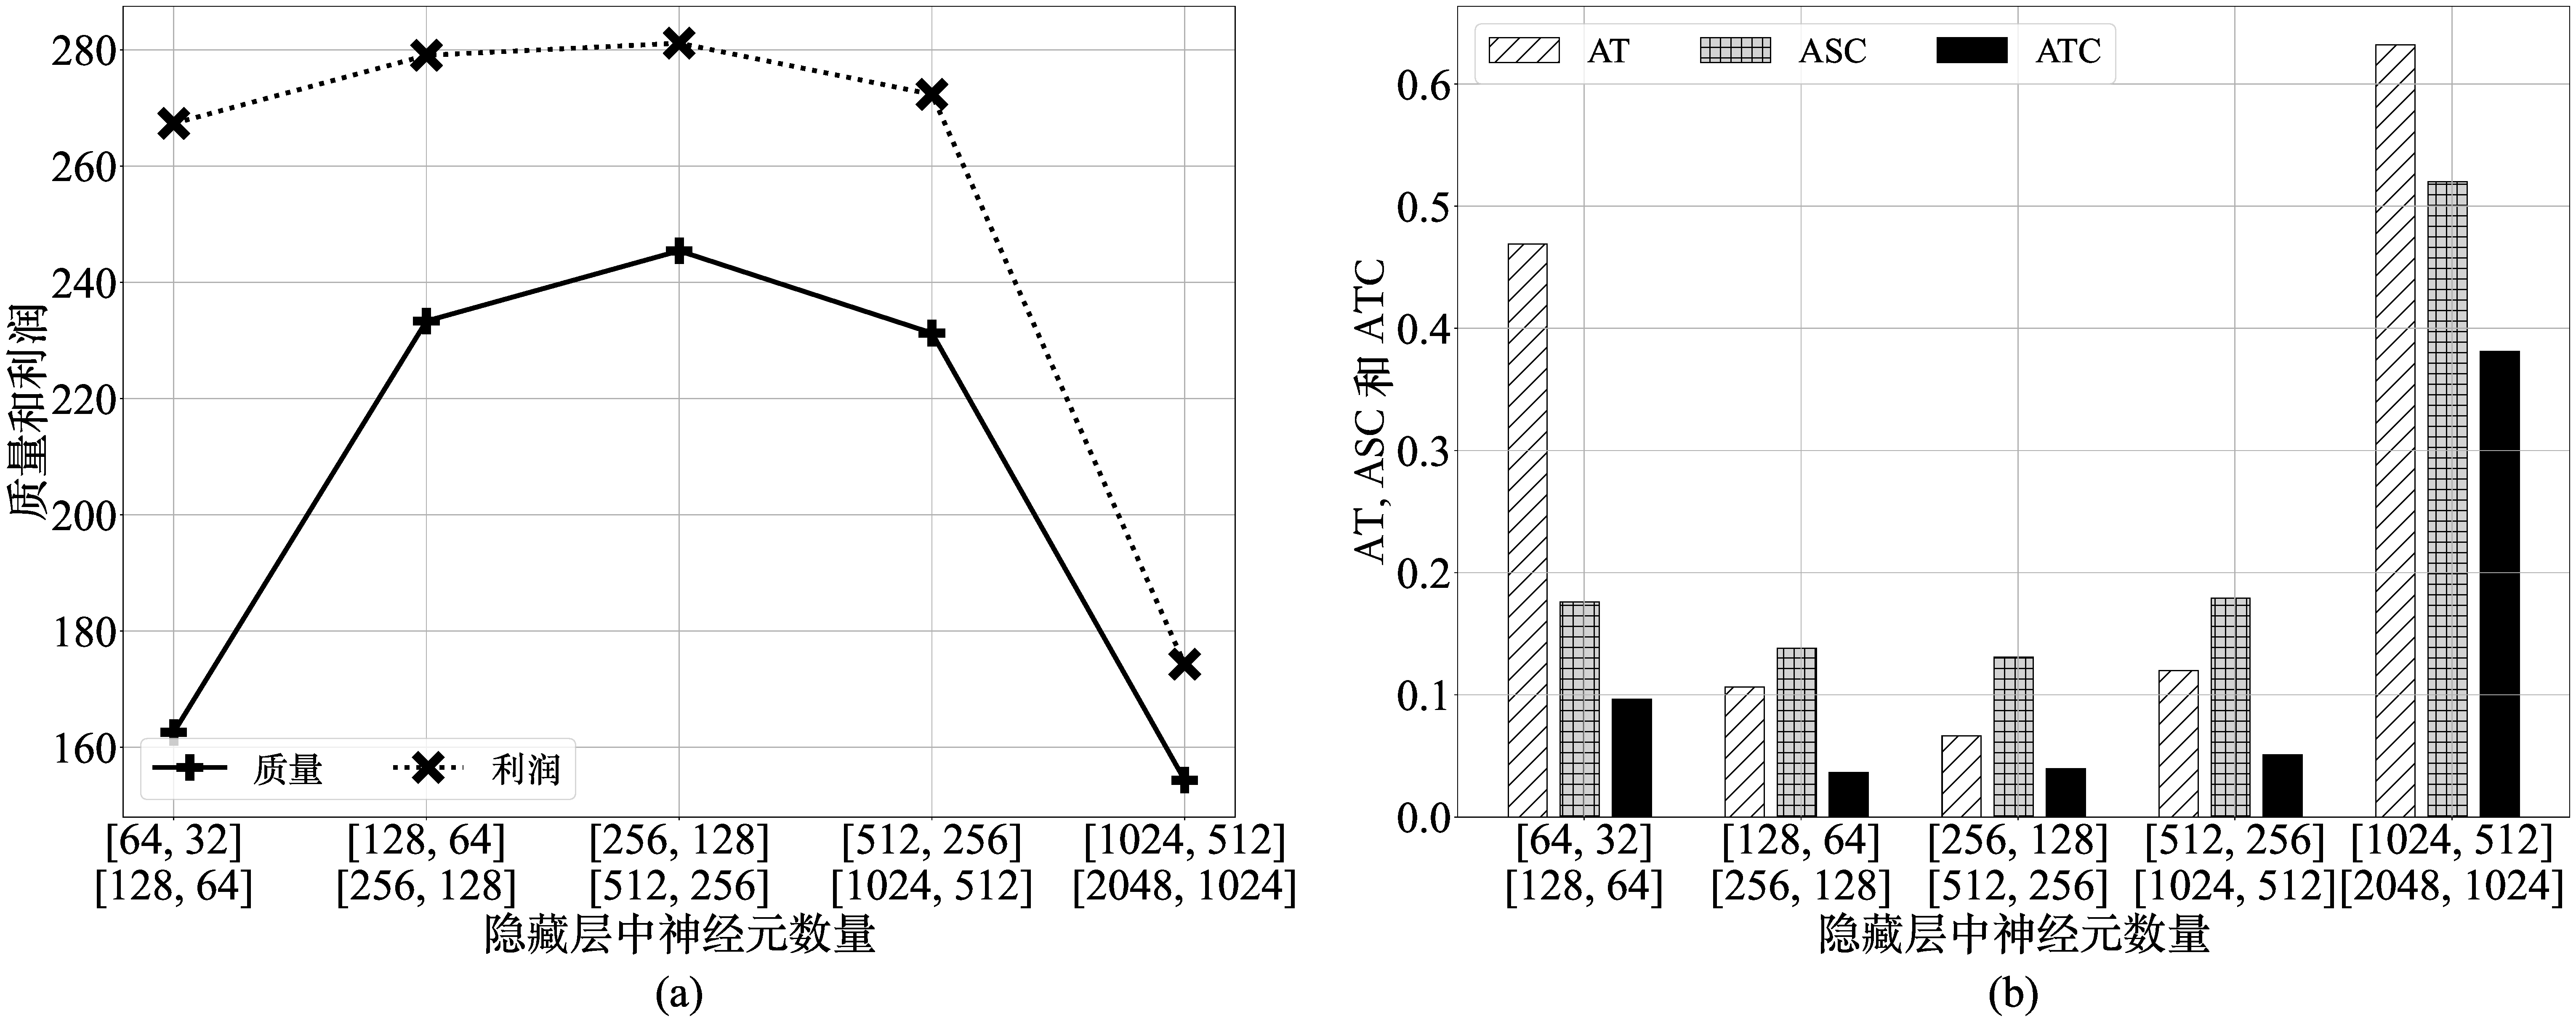
\includegraphics[width=1\columnwidth]{Fig4-4-different-networks.pdf}
 \bicaption[隐藏层中不同数量神经元下MAMO性能比较]{隐藏层中不同数量神经元下MAMO性能比较。(a)单位开销质量(b)单位质量利润}[Performance comparison of MAMO under different numbers of neurons in the hidden layers]{Performance comparison of MAMO under different numbers of neurons in the hidden layers. (a) Quality per unit cost (b) Profit per unit quality}
 \label{fig 4-4}
\end{figure}

\textbf{2) 神经元数量的影响:}
图\ref{fig 4-4}比较了不同神经元数量下MAMO的性能。其中,X轴表示策略网络和评论家网络的两个隐藏层的神经元数量,分别设置为[64, 32] $\sim$ [1024, 512]和[128, 64] $\sim$ [2048, 1024]。如图\ref{fig 4-4}(a)所示,当策略网络和评论家网络的隐藏层的神经元数量设置为默认值(即[256, 128]和[512, 256])时,MAMO实现了最高的VCPS质量和利润。图\ref{fig 4-4}(b)比较了其他三个指标,包括AT、ASC和ATC。AT、ASC和ATC越低,说明在信息新鲜度、感知开销和传输开销方面表现越好。可以注意到,当每个隐藏层的神经元数量为默认设置时,MAMO在最小化AT、ASC和ATC方面表现最佳。

\begin{figure}[h]
 \centering
 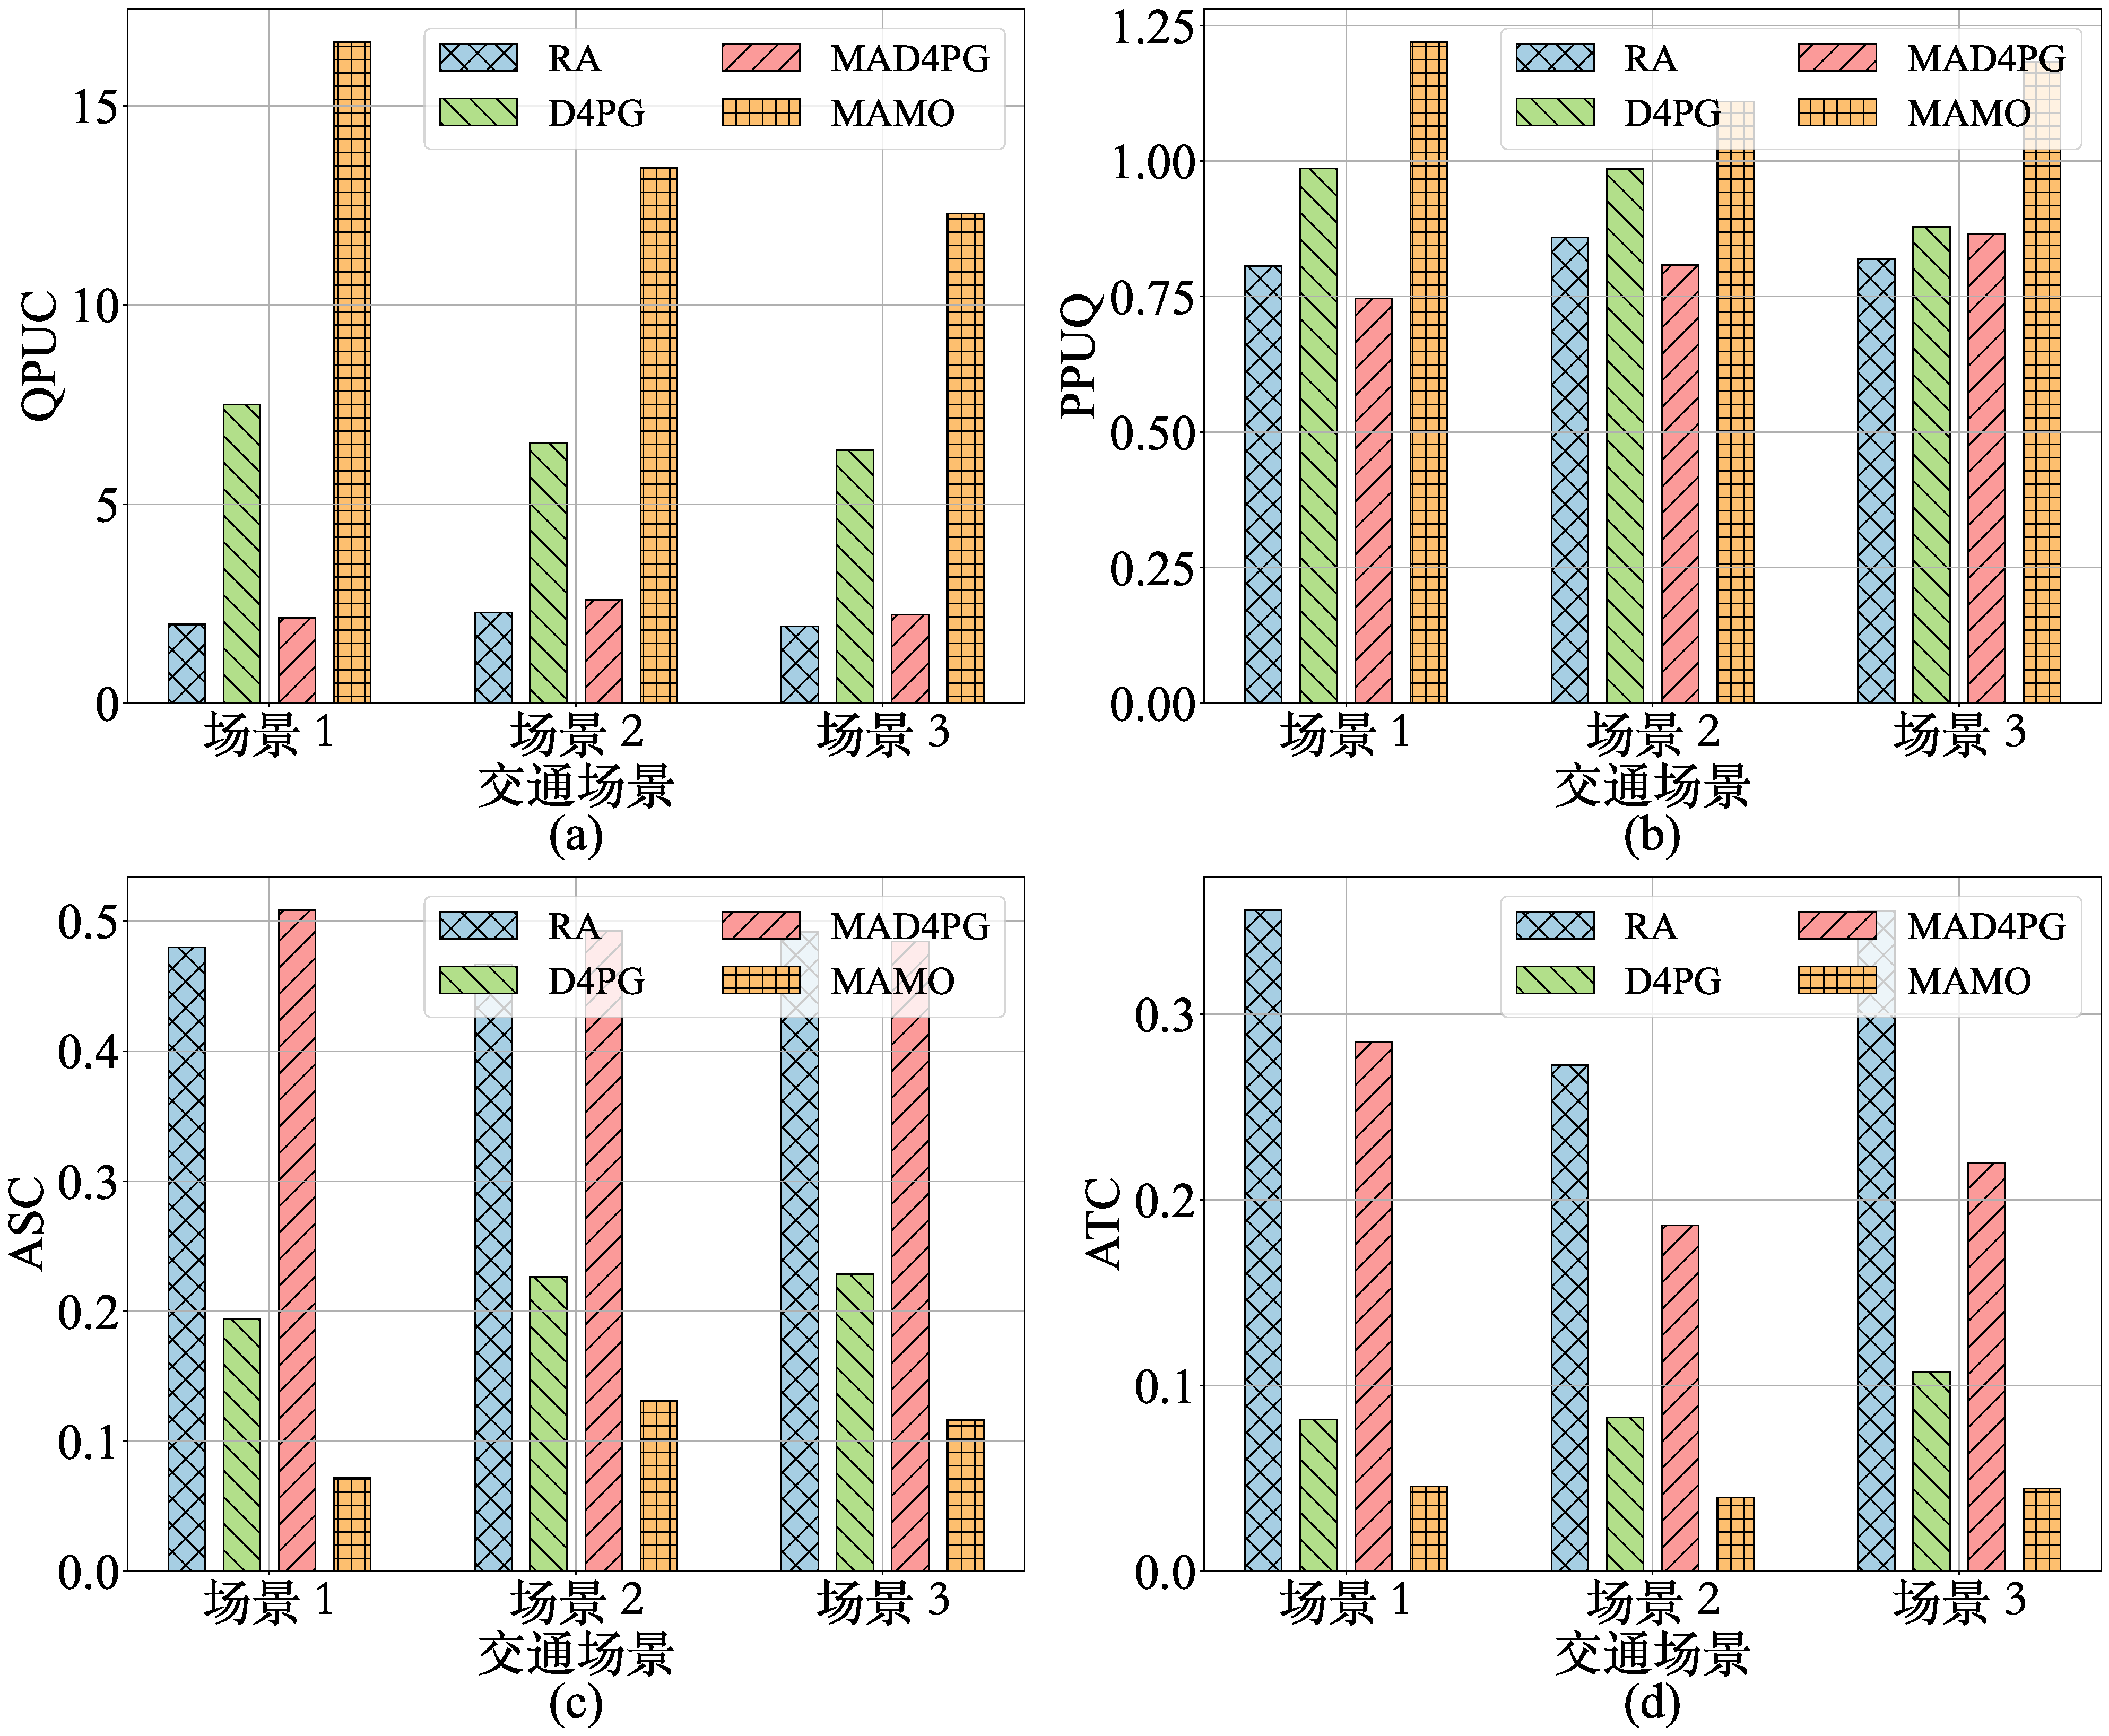
\includegraphics[width=1\columnwidth]{Fig4-5-different-scenarios.pdf}
 \bicaption[不同交通场景下的性能比较]{不同交通场景下的性能比较。(a)单位开销质量(b)单位质量利润(c)平均感知开销(d)平均传输开销}[Performance comparison under different traffic scenarios]{Performance comparison under different traffic scenarios. (a) Quality per unit cost (b) Profit per unit quality (c) Average sensing cost (d) Average transmission cost}
 \label{fig 4-5}
\end{figure}

\textbf{3) 交通情况的影响:}
图\ref{fig 4-5}比较了四种算法在不同交通场景下的性能。X轴表示交通场景,不同场景在不同的时间和空间中提取了现实的车辆轨迹作为输入,分别为:1)2016年11月16日8:00至8:05,中国成都市青羊区1平方公里区域;2)同日23:00至23:05,同一区域;3)2016年11月27日8:00至8:05,中国西安碑林区1平方公里区域。图\ref{fig 4-5}(a)比较了四种算法的QPUC,MAMO在所有场景下都取得了最高的QPUC。图\ref{fig 4-5}(b)比较了四种算法的PPUQ,MAMO在所有情况下都表现最好。与RA、D4PG和MAD4PG相比,MAMO分别提高了589.0\%、106.7\%和514.8\%的QPUC,并分别提高了约41.6\%、23.6\%和45.7\%的PPUQ。图\ref{fig 4-5}(c)比较了四种算法的ASC。MAMO的ASC低于RA、D4PG和MAD4PG,说明MAMO可以实现车辆协同感知以降低感知开销。图\ref{fig 4-5}(d)比较了四种算法的ATC,在不同情况下,MAMO的ATC最低。

\begin{figure}[h]
 \centering
 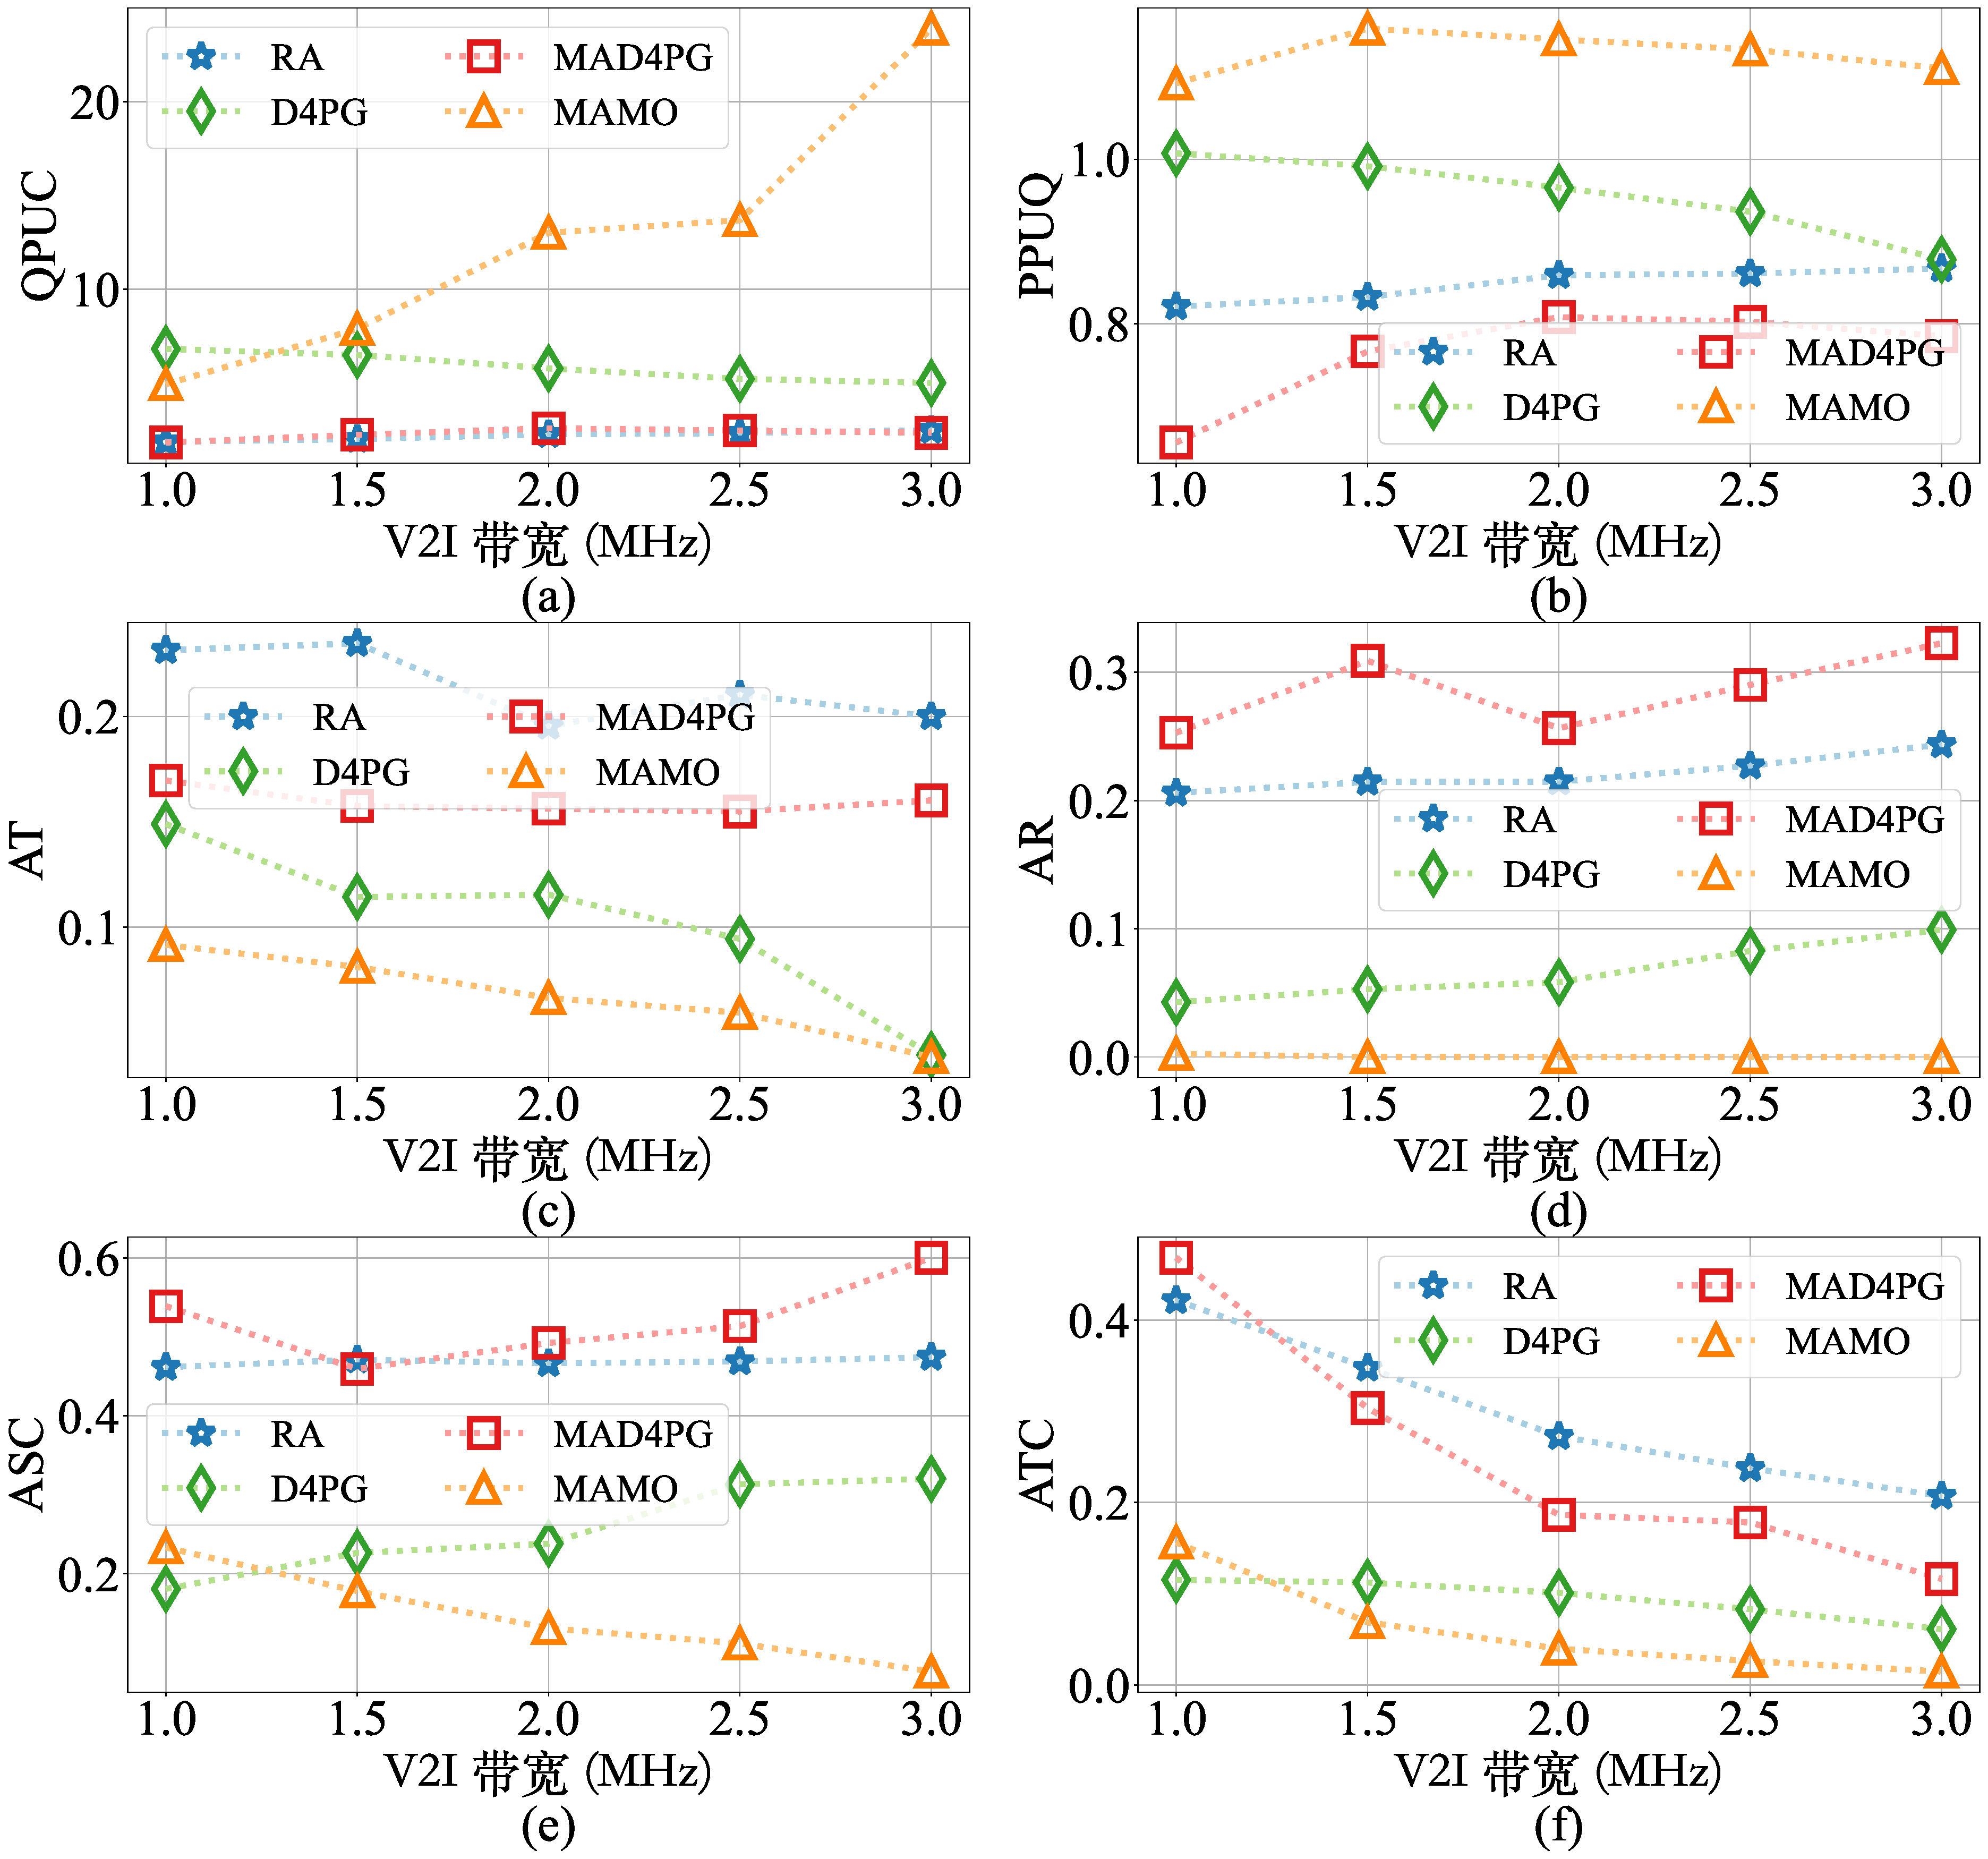
\includegraphics[width=1\columnwidth]{Fig4-6-different-bandwidths.pdf}
 \bicaption[不同V2I带宽下的性能比较]{不同V2I带宽下的性能比较。(a)单位开销质量(b)单位质量利润(c)平均及时性(d)平均冗余度(e)平均感知开销(f)平均传输开销}[Performance comparison under different V2I bandwidths]{Performance comparison under different V2I bandwidths. (a) Quality per unit cost (b) Profit per unit quality (c) Average timeliness (d) Average redundancy (e) Average sensing cost (f) Average transmission cost}
 \label{fig 4-6}
\end{figure}

\begin{figure}[h]
 \centering
 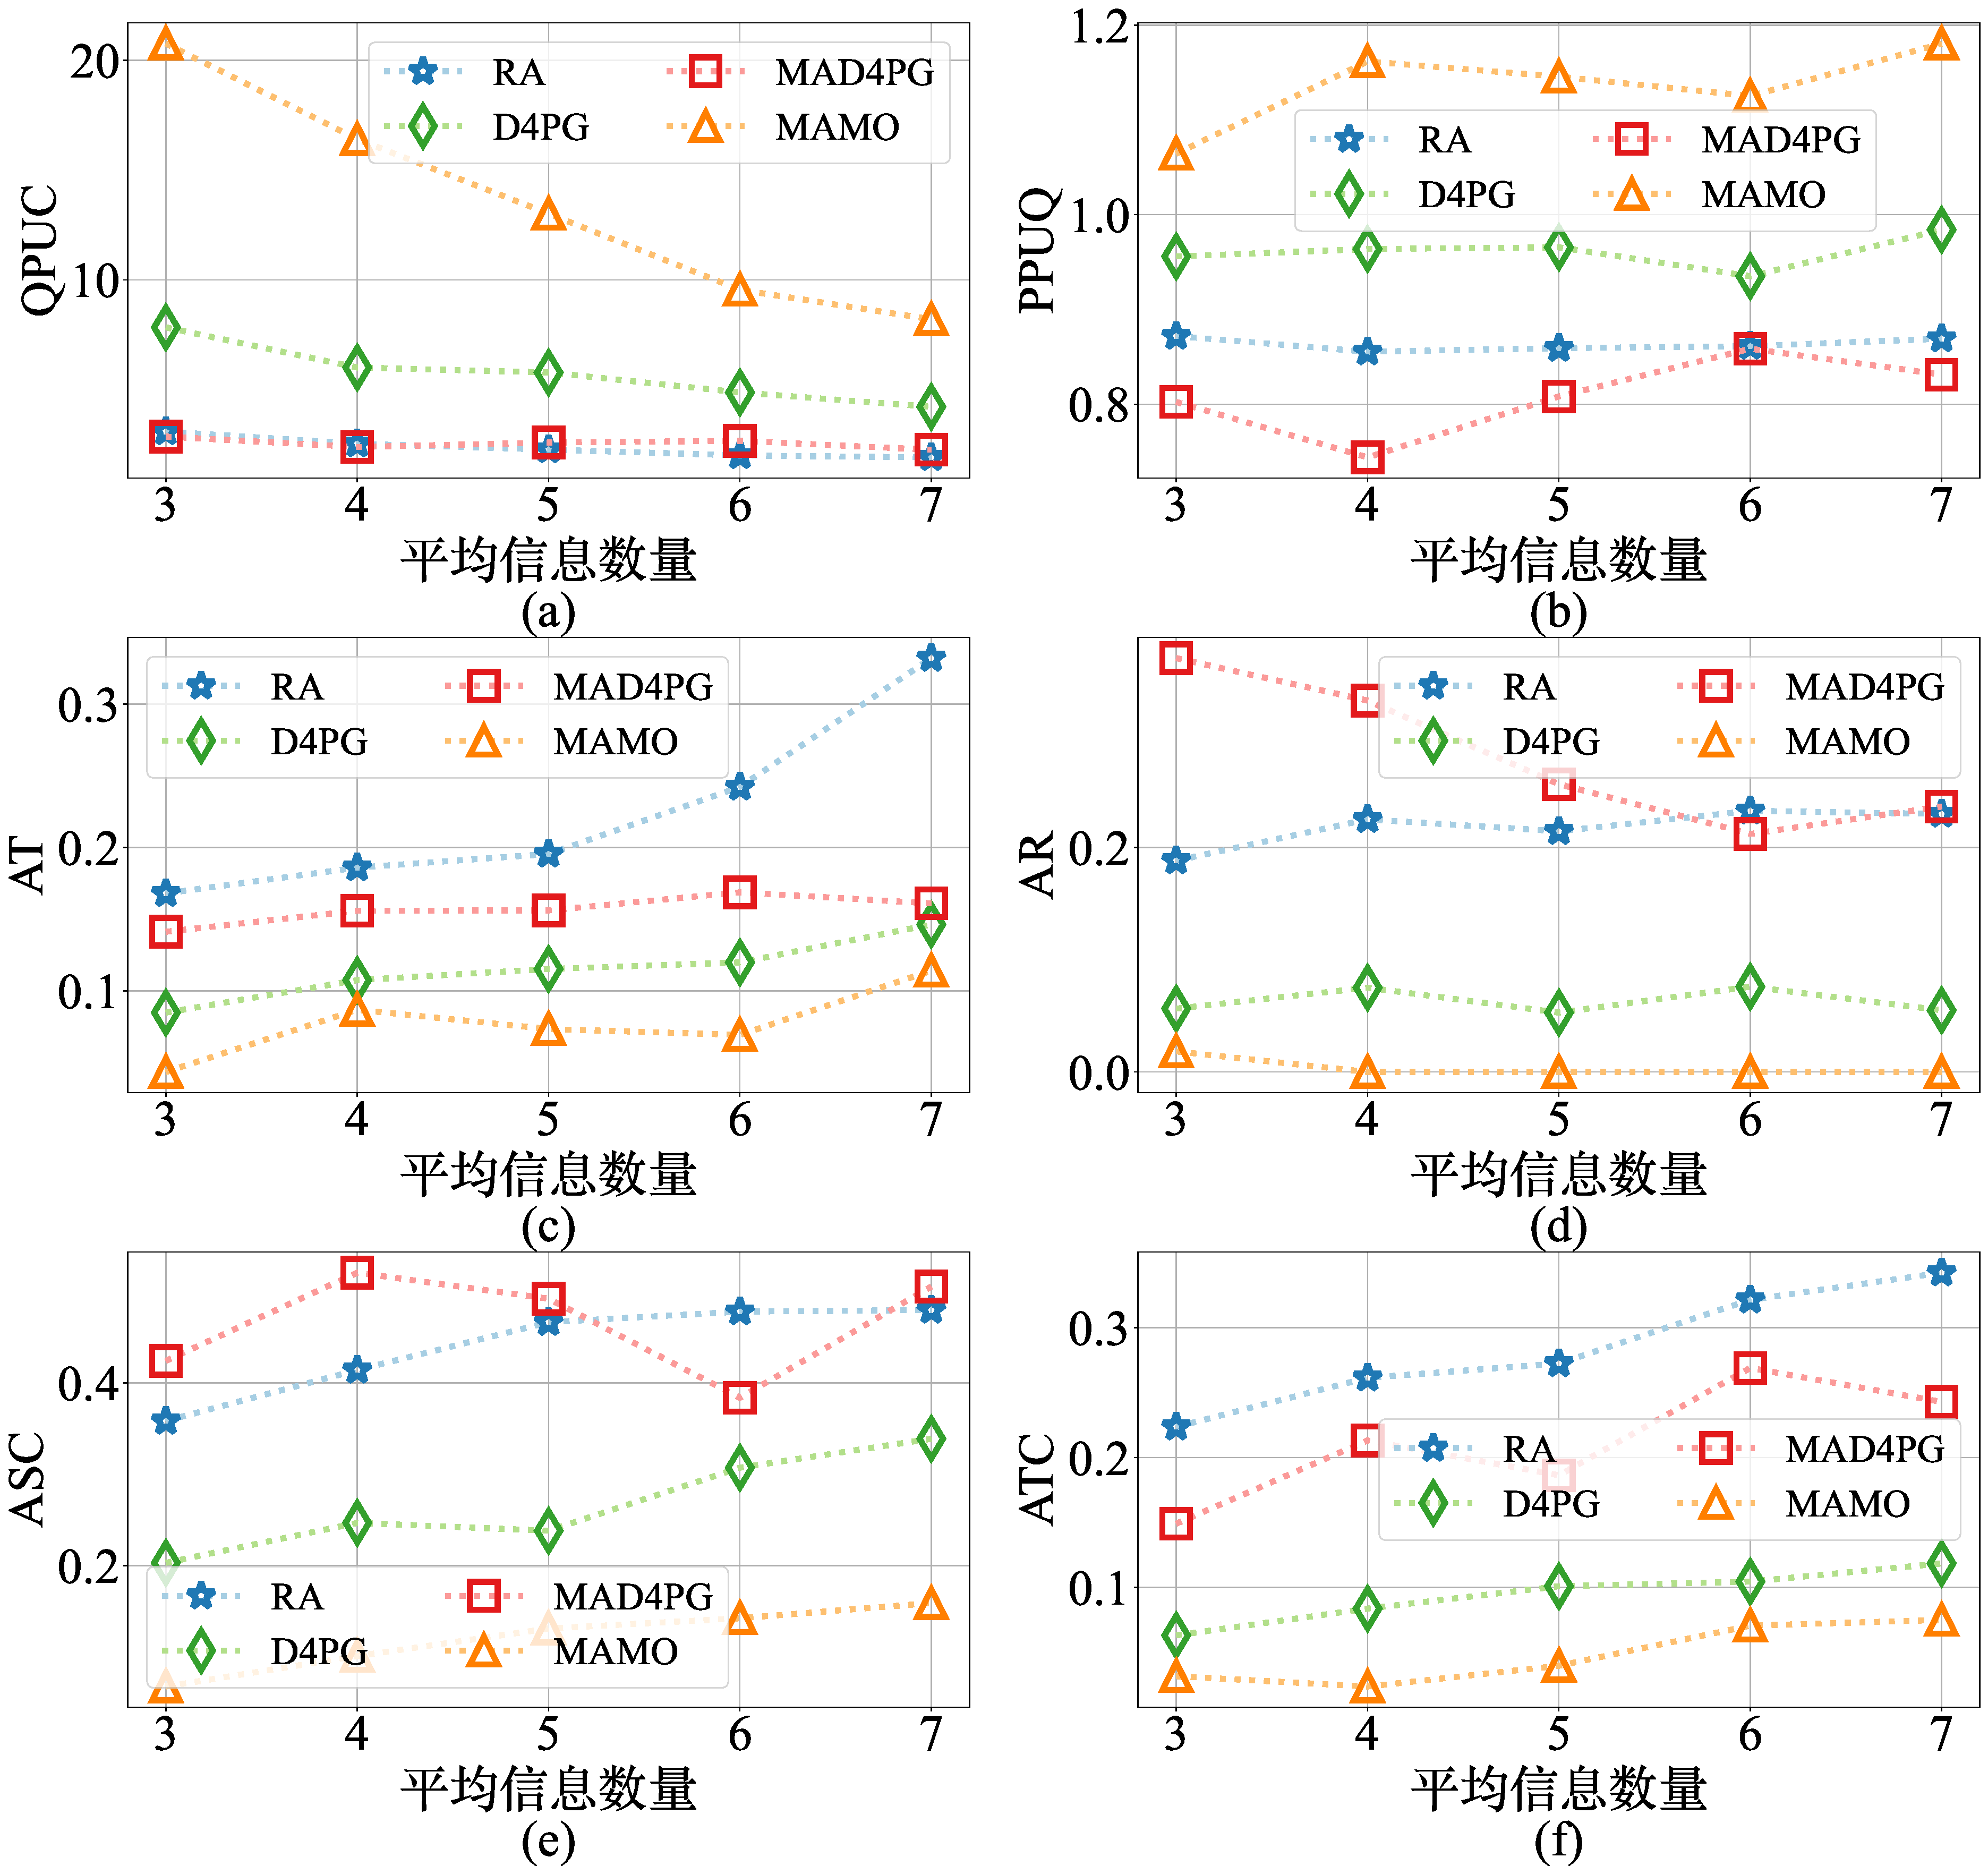
\includegraphics[width=1\columnwidth]{Fig4-7-different-numbers.pdf}
 \bicaption[不同视图需求下的性能比较]{不同视图需求下的性能比较。(a)单位开销质量(b)单位质量利润(c)平均及时性(d)平均冗余度(e)平均感知开销(f)平均传输开销}[Performance comparison under different digit twin requirements]{Performance comparison under different digit twin requirements. (a) Quality per unit cost (b) Profit per unit quality (c) Average timeliness (d) Average redundancy (e) Average sensing cost (f) Average transmission cost}
 \label{fig 4-7}
\end{figure}

\textbf{4) V2I带宽的影响:}
图\ref{fig 4-6}比较了四种算法在不同V2I带宽下的性能。X轴表示V2I带宽,从1MHz增加到3MHz。较大的V2I带宽代表每辆车被分配的V2I带宽也随之增加。图\ref{fig 4-6}(a)比较了四种算法的QPUC。随着带宽的增加,MAMO的QPUC也相应增加。这是因为在带宽富余的场景中,MAMO中车辆之间的协同感知和上传更加有效。图\ref{fig 4-6}(b)显示了四种算法的PPUQ,可以进一步证明这一优势。如图\ref{fig 4-6}(b)所示,MAMO在不同的V2I带宽下实现了最高的PPUQ。特别地,与RA、D4PG和MAD4PG相比,MAMO分别提高了约453.3\%、131.4\%和437.6\%的QPUC,并使PPUQ提高了约33.0\%、18.3\%和48.4\%。图\ref{fig 4-6}(c)比较了四种算法的AT,MAMO实现了最低的AT。当带宽从2.5MHz增加到3MHz时,MAMO和D4PG的性能差距很小。这是因为随着带宽的增加,视图的及时性改善是有限的。图\ref{fig 4-6}(d)比较了四种算法的AR。AR越低意味着协同感知和上传的性能越好,MAMO实现了最低的AR。图\ref{fig 4-6}(e)和\ref{fig 4-6}(f)分别比较了四种算法的ASC和ATC。可以看出,当带宽增加时,这四种算法的ATC都会下降。原因是,当带宽增加时,信息上传时间减少,导致传输开销降低。MAMO的ASC和ATC在大多数情况下保持在最低水平。

\textbf{5) 视图需求的影响:}
图\ref{fig 4-7}比较了四种算法在不同视图需求下的性能,其中X轴表示视图所需信息的平均数量从3增加到7。视图所需信息的平均数越大,说明车辆的感知和上传工作负荷越大。图\ref{fig 4-7}(a)比较了四种算法的QPUC。随着平均所需信息数的增加,四种算法的QPUC也相应减少。然而,MAMO在所有情况下保持最高的QPUC。图\ref{fig 4-7}(b)比较了四种算法的PPUQ。正如预期的那样,MAMO在所有情况下都取得了最高的PPUQ。特别地,与RA、D4PG和MAD4PG相比,MAMO的QPUC分别高出458.7\%、130.6\%和426.2\%,PPUQ分别高出31.5\%、18.2\%和40.7\%。图\ref{fig 4-7}(c)比较了四种算法的AT。MAMO在AT方面取得了最佳性能。图\ref{fig 4-7}(d)比较了四种算法的AR,表明MAMO可以在所有情况下实现最低的AR。图\ref{fig 4-7}(e)和\ref{fig 4-7}(f)分别比较了四种算法的ASC和ATC。值得注意的是,当平均信息数增加时,四种算法的ASC和ATC都会增加。原因是视图需要的平均信息量增加,导致车辆感应和传输开销提高。

\section{本章小结}\label{section 4-7}

本章提出了协同感知与V2I上传场景,其中基于车辆协同感知与V2I协同上传构建逻辑视图。
具体地,基于多类M/G/1优先级队列构建了协同感知模型,并基于信道衰减分布和SNR阈值构建了V2I协同上传模型。
在此基础上,设计了两个指标QV和CV,以衡量在边缘节点建模的视图的质量和开销,并形式化定义了一个双目标优化问题,通过协同感知和上传,最大化VCPS质量的同时,最小化VCPS 开销。
进一步,提出了一个基于多目标的多智能体深度强化学习算法,其中采用了一个决斗评论家网络,根据状态价值和动作优势来评估智能体动作。
最后,进行了全面的性能评估,证明了所提MAMO算法的优越性。
\chapter[面向车载信息物理融合的超视距碰撞预警原型系统设计及实现]{面向车载信息物理融合的超视距碰撞预警原型系统\\设计及实现}
本章将研究面向车载信息物理融合的超视距碰撞预警原型系统设计及实现。
内容安排如下:
\ref{section 5-1} 节是本章的引言,介绍了车联网碰撞预警系统研究现状和目前研究的不足以及本章的主要贡献。
\ref{section 5-2} 节介绍了超视距碰撞预警场景。
\ref{section 5-3} 节设计了基于视图修正的碰撞预警算法。
\ref{section 5-4} 节构建了基于真实车辆轨迹的仿真实验模型,并验证了所提算法的性能。
\ref{section 5-5} 节搭建了基于C-V2X设备的硬件在环试验平台,并在真实车联网环境实现了超视距碰撞预警原型系统,并对所提算法与系统进行了可行性与有效性验证。
\ref{section 5-6} 节总结了本章的研究工作。

\section{引言}\label{section 5-1}

车辆碰撞预警系统作为 ITS 的典型安全应用,已得到学术界与工业界的广泛关注。
现有大多数车辆碰撞预警系统都基于超声波雷达或激光雷达等测距传感器进行实现\cite{song2018real, wu2019series},并取得了不错的效果,但是这些方案都存在非视距的问题。
随着近年来计算机视觉的发展,部分研究尝试利用车载摄像头的实时视频流来进行车辆碰撞检测 \cite{wang2016vision, song2018lane}。
然而,基于计算机视觉的方法需要大量数据传输和密集计算,这对系统性能提出了更高的要求,在实际部署中无法保证系统的实时响应。 
部分研究基于车联网通信实现碰撞预警\cite{hafner2013cooperative, gelbal2017elastic}。
但是,无线通信中传输时延和数据包丢失等问题是不可避免的,而车辆碰撞预警系统对实时性具有非常严苛的要求,这使得在车联网中实现实时可靠的安全关键型服务变得更加困难。
因此,面向真实复杂性车联网通信环境,如何有效获得实时准确的边缘视图,在此基础上,提供高质量的碰撞预警服务是具有挑战性与实用价值的。

基于以上分析,本章致力于设计及实现真实复杂性车联网环境中超视距碰撞预警原型系统。
本章的主要贡献总结如下:
第一,提出了基于视图修正的碰撞预警(View-Calibration-based Collision Warning, VCCW)算法,其通过结合通信时延估计和丢包检测来修正视图,从而提高碰撞预警系统的及时性和准确性。
具体地,基于真实车联网环境开展了现场测试并得到了 V2I 通信应用层时延数据,在此基础上,对车联网V2I通信的传输时延进行拟合,推导出了基于稳定分布的传输时延拟合模型。
另一方面,根据车辆位置和数据传输频率的历史信息,设计了一个丢包检测机制。
第二,基于真实车辆轨迹建立了仿真实验模型。
具体地,在德国科隆市选取具有不同特征(如交通密度、车辆速度、车辆加速度)的交叉路口并导入真实世界的车辆轨迹。
实现了所提算法与两种传统算法,其中包括基于云的碰撞预警(Cloud-Based Collision Warning, CCW)和基于边缘的碰撞预警(Edge-Based Collision Warning, ECW)。
CCW 和 ECW 均未考虑对视图进行修正。
仿真实验结果表明,与传统方法相比,VCCW 在碰撞预警的查全率、查准率以及F1值方面都具有优势。
第三,基于 C-V2X 通信设备,搭建了硬件在环试验平台,并分析了不同数据包大小对 C-V2X 端到端传输时延的影响。
进一步,在真实车联网环境中,实现了基于车载信息物理融合的超视距碰撞预警原型系统,验证了本系统的可行性与有效性。

\section{超视距碰撞预警场景}\label{section 5-2}

本章将介绍超视距碰撞预警场景,如图 \ref{fig 5-1} 所示,具有短无线电覆盖范围的通信基础设施(如RSU、5G小基站)作为边缘节点,其在物理位置上更接近车辆并具有一定的计算能力。
同时,具有广泛覆盖范围的通信基础设施(如 5G 蜂窝网络基站)作为云节点。
车辆可通过 V2C 和 V2I 通信分别与云节点和路侧边缘节点进行通信。
虽然云节点拥有足够强大的算力来满足其覆盖范围内所有车辆的任务请求,但也会受到通信带宽的限制,如果当前云节点服务的车辆进行并发的数据传输,极大可能产生严重的带宽竞争,造成系统的吞吐量急剧下降。
与传统的基于云的服务相比,基于车载边缘计算的服务不仅减少了无线通信时延,而且通过将计算任务卸载到分布式的边缘节点上,提高了系统的响应性和可扩展性。
在本场景中,两辆汽车(即 $v_1$ 和 $v_2$)正从两个方向接近没有交通信号灯的十字路口。
在两车均不在对方视野的情况下,发生碰撞事故的概率大大增加。
为避免上述事故的发生,需要实现非视距场景下的车辆碰撞预警,因此,本章提出了基于逻辑视图的超视距碰撞预警系统。
车辆定期通过 V2I 通信将实时状态上传至边缘节点,包括全球定位系统(Global Positioning System, GPS)坐标、速度、加速度、方向等。
随后,边缘节点对覆盖范围内的车辆传感数据进行处理,构建出反映车辆实时状态的逻辑视图,以支持基于车辆轨迹预测的碰撞预警服务。
然而,车辆传感数据容易受到外界条件影响而出现偏差。
例如,由于卫星时钟偏差、大气时延和广播星历错误等原因,获得的 GPS 坐标可能出现偏移 \cite{liu2013improving}。
此外,数据包丢失也使边缘节点对移动车辆的实时位置估计变得更加困难。

\begin{figure}[h]
	\centering
	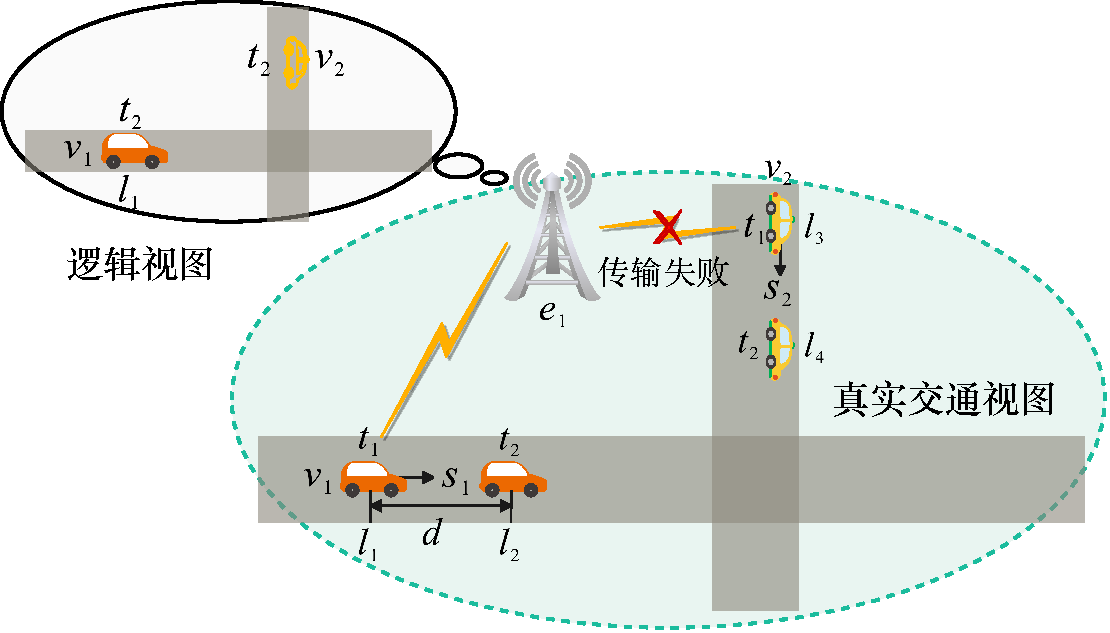
\includegraphics[width=0.9\columnwidth]{Fig5-1-example.pdf}
	\bicaption{超视距碰撞预警场景}{None-light-of-sight collision warning scenario}
	\label{fig 5-1}
\end{figure}

综上所述,尽管移动边缘计算新范式比传统的集中式云计算减少了通信时延,但由于不可避免且难以忽视的诸如传感器错误、传输时延和数据包丢失等问题,面向碰撞预警系统的边缘视图的有效构建仍然存在严峻的挑战。
图 \ref{fig 5-1} 显示了边缘节点构建的逻辑视图与真实交通视图的差异,其本质原因是边缘节点对车辆位置的不准确估计。
具体来说,假设车辆$v_1$在时间$t_1$的位置为$l_1$,且以$s_1 =$ 40 km/h 的速度接近十字路口。
同时,车辆$v_2$在时间$t_1$位于$l_3$并以$s_2=$ 25 km/h的速度接近同一路口。
车辆$v_1$和$v_2$在时间$t_1$同时向边缘节点发送实时状态。
然而,包含车辆$v_2$状态的数据包在V2I通信中丢失。
边缘节点在时间$t_2$接收到车辆状态信息,并形成车辆位置分布的逻辑视图,如图\ref{fig 5-1}所示。
假设数据大小为 500 kB,这对于典型的ITS应用来说是足够的\cite{liu2013improving}。
典型的车联网通信技术DSRC支持3$\sim$27 Mb/s的传输速率,其中3 Mb/s 被推荐用于传输安全关键信息\cite{kenney2011dedicated}。
因此,车辆状态的上传时间约为500 * 8 kb / 3 $\approx$ 1.3 s,即${t_2} - {t_1} \approx 1.3$ s。
在逻辑视图中,车辆$v_1$位于$l_1$,而$v_2$不存在。
然而如真实交通视图所示,车辆$v_1$和$v_2$的真实位置分别为$l_2$和$l_4$。
车辆$v_1$在逻辑车辆视图和真实交通视图之间的位置误差约为40 * 1000 / 3600 m/s * 1.3 $\approx$ 14 m,换言之,$d \approx$ 14 m。
从上述例子可以看出,如何在车联网中实现信息物理融合即构建一个实时准确的视图以支持不同的智能交通系统应用是迫切需要解决且极具挑战的问题。

\section{基于视图修正的碰撞预警算法}\label{section 5-3}

本章节提出了基于视图修正的碰撞预警算法,其通过拟合传输时延和检测丢包来修正边缘节点构建的逻辑视图,以提高碰撞预警的服务质量。
首先,基于真实车联网环境测试数据对V2I应用层传输时延进行拟合,得到基于稳定分布的V2I时延模型。
其次,基于数据传输频率和车辆位置的历史信息,设计了丢包检测机制。
最后,阐述了基于视图修正的碰撞预警算法的详细工作流程。

\subsection{应用层V2I时延拟合模型}

\begin{figure}[h]
\centering
  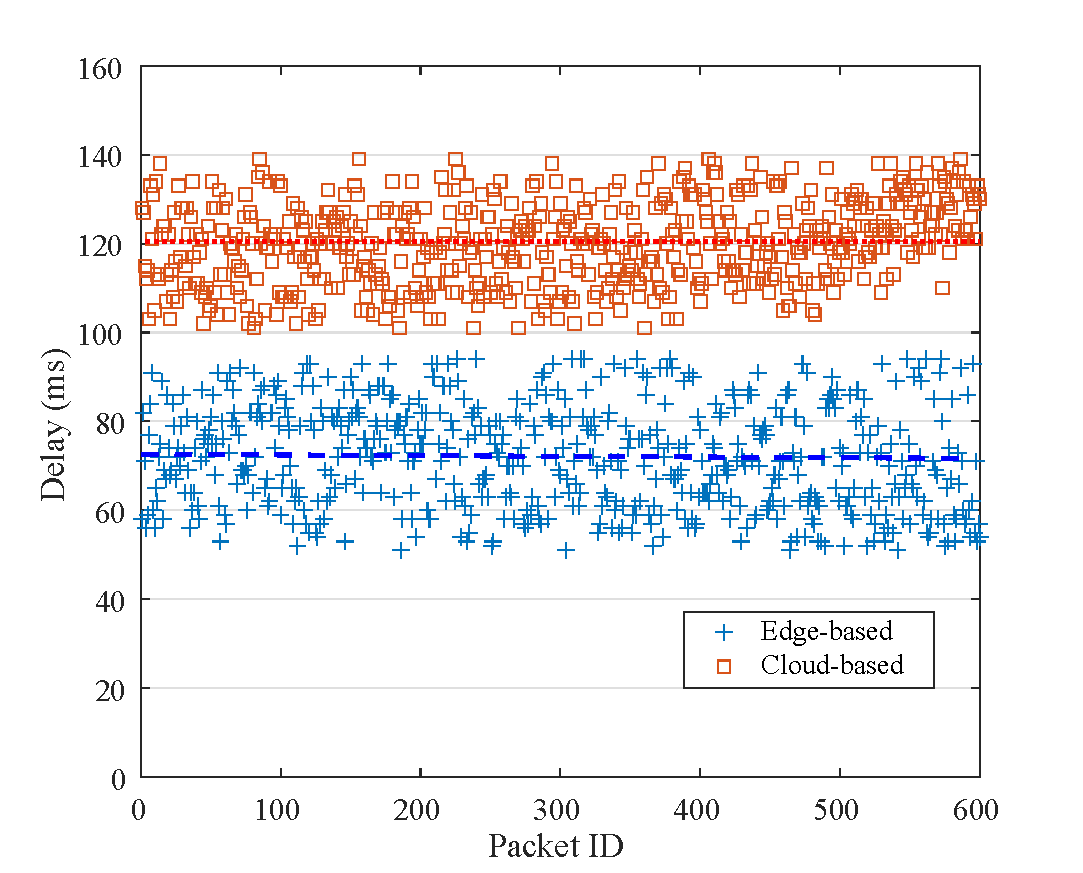
\includegraphics[width=0.8\columnwidth]{Fig5-2-delay.pdf}
  \bicaption[不同系统架构下的传输时延]{不同系统架构下的传输时延,云计算和车载边缘计算中数据包传输的平均时延分别为120${ms}$和77${ms}$}[Transmission delay under different system architectures]{Transmission delay under different system architectures where average delay of packets transmission in cloud and fog computing is 120 ms and 77 ms, respectively}
  \label{fig 5-2}
\end{figure}

本章根据真实车联网环境的现场测试数据分析了V2I通信的应用层传输时延。
在现场测试中,配备OBU的车辆通过V2I通信与RSU通信。
RSU作为边缘节点被安装在十字路口,与之相连的笔记本电脑充当RSU的计算单元。
当车辆接近十字路口时,通过V2I通信定期发送车辆状态,包括GPS坐标、速度、加速度、方向和时间戳。
边缘节点接收车辆数据包并计算V2I通信的应用层传输时延。
接下来,本章对真实车联网通信环境中的V2I传输时延进行建模。
具体地,根据对传输时延测试结果的观察,发现V2I通信的应用层传输时延分布并不服从高斯分布,而稳定分布是一种成熟的模型,适用于对非高斯过程进行估计。
本章节末尾的拟合结果表明,稳定分布可以相当准确地描述传输时延的特征和性质。
因此,本章利用稳定分布来拟合应用层V2I通信时延,其可以用如下的特征函数\cite{samoradnitsky2017stable}来描述
\begin{numcases}{E \exp (i t X)=}
\exp \left\{-\sigma^{\alpha}|t|^{\alpha}[1-i \beta \tan (\alpha \pi / 2) \operatorname{sgn}(t)]+i \mu t\right\}, &$\alpha \neq 1$ \notag \\
\exp \{-\sigma|t[1+i \beta(2 / \pi) \operatorname{sgn}(t) \ln (|t|)]+i \mu t\},  &$\alpha=1$
\end{numcases}
\noindent
其中 $X$ 是一个随机变量并服从稳定分布 $X \sim {S(\alpha, \beta, \mu, \sigma)}$, 且
\begin{numcases}{}
	\alpha \in \left( 0, 2\right] \notag \\
	\beta \in \left[ -1, 1 \right] \notag \\
	\mu \in \mathbb{R} \notag \\
	\sigma \in \mathbb{R}^{+}
\end{numcases}
其中$\alpha$是稳定性指数,当$\alpha=2$时,该稳定分布是高斯分布。
$\beta$是一个偏度参数,当$\beta=0$时,该稳定分布具有中心对称性,其对称中心为$\mu$。
$\alpha \neq 1$,$\beta > 0$和$\beta < 0$的情况分别对应于左偏度和右偏度。
$\sigma$是一个类似于方差的尺度参数。
特征函数$\phi(t)=E \exp (i t X)$完全决定了随机变量$X$概率分布的行为和特性,其中$t$为实数,$i$为虚数单位,$E$为期望值。
$\operatorname{sgn}(t)$ 是一个符号函数,其定义为:
\begin{numcases}{\operatorname{sgn}(t)=}
		1, &$t>0$ \notag \\
		0, &$t=0$ \notag \\
		-1, &$t<0$ 
\end{numcases}

本章采用回归模型来估计稳定分布的四个参数。
首先,给定大小为$n$的观测数据随机样本,记为$x_1, x_2, \ldots, x_n$,那么特征函数$\hat{\phi}(t)$可定义为
\begin{align}
	\hat{\phi}(t)&\!=\!\frac{1}{n} \sum_{j=1}^{n} \exp \left(i t x_{j}\right) \notag \\
	&\!=\!\frac{1}{n} \sum_{j=1}^{n}\left[\cos \left(t x_{j}\right)+\sin \left(t x_{j}\right) i\right] \notag \\
	&\!=\!\frac{1}{n} \sum_{j=1}^{n} \cos \left(t x_{j}\right)+i \frac{1}{n} \sum_{j=1}^{n} \sin \left(t x_{j}\right)
\end{align}
当 $\alpha \neq 1$, 可以得到
\begin{align}
	\phi(t) 
	&\!=\!E \exp (i t X) \notag \\ 
	&\!=\!\exp \left\{-\sigma^{\alpha}|t|^{\alpha}[1\!-\!i \beta \tan (\alpha \pi / 2) \operatorname{sgn}(t)]+i \mu t\right\} \notag \\ 
	&\!=\!\exp \left\{-\sigma^{\alpha}|t|^{\alpha}\!+\!\left[\mu t\!+\!\sigma^{\alpha}|t|^{\alpha} \beta \tan (\alpha \pi / 2) \operatorname{sgn}(t)\right] i\right\} \notag \\  
	&\!=\!\exp \left(-\sigma^{\alpha}|t|^{\alpha}\right) \exp \left[\left(\mu t\!+\!\sigma^{\alpha}|t|^{\alpha} \beta \tan (\alpha \pi / 2) \operatorname{sgn}(t)\right] i\right\} \notag \\ 
	&\!=\!\exp \left(-\sigma^{\alpha}|t|^{\alpha}\right) \cos \left[\mu t\!+\!\sigma^{\alpha}|t|^{\alpha} \beta \tan (\alpha \pi / 2) \operatorname{sgn}(t)\right] \notag \\ 
	&\!+\!\exp \left(-\sigma^{\alpha}|t|^{\alpha}\right) \sin \left[\mu t\!+\!\sigma^{\alpha}|t|^{\alpha} \beta \tan (\alpha \pi / 2) \operatorname{sgn}(t)\right] i 
\label{equ 5-5}
\end{align}
假设分布围绕中心$0$对称(即$\beta = 0$,$\mu = 0$),容易得到
\begin{equation}
	-\ln |\phi(t)|^{2}=2 \sigma^{\alpha}|t|^{\alpha}
\end{equation}
进一步可得
\begin{align} 
	\ln \left(-\ln | \phi(t)^{2}\right)
	&= \ln \left(2 \sigma^{\alpha}|t|^{\alpha}\right) \notag \\ 
	&=\ln \left(2 \sigma^{\alpha}\right)+\alpha \ln (|t|) 
\end{align}


通过回归$y_{k}=\alpha \omega_{k}+b$来估计$\alpha$和$\sigma$,其中${b=\ln \left(2 \sigma^{\alpha}\right)}$和${\omega_{k}=\ln \left(\left|t_{k}\right|\right)}$。
记$f\left(t_{k}\right)=\ln \left(-\ln \left|\phi\left(t_{k}\right)\right|^{2}\right)$并使用线性回归最小化均方误差。
\begin{align}
\left(\alpha^{*}, b^{*}\right) &=\underset{(\alpha, b)}{\arg \min } \sum_{k=1}^{K}\left(f\left(t_{k}\right)-y_{k}\right)^{2} \notag \\ &=\underset{(\alpha, b)}{\arg \min } \sum_{k=1}^{K}\left[\ln \left(-\ln \left|\phi\left(t_{k}\right)\right|^{2}\right)-\left(\alpha \omega_{k}+b\right)\right]^{2}  
\end{align}
然后,用最小平方法得到估计值$\hat{\alpha}$和$\hat{\sigma}$,即
$E_{(\alpha, b)}=\sum_{k=1}^{K}\left(f\left(t_{k}\right)-y_{k}\right)^{2}$,其中估计参数可通过求解下式获得。
\begin{numcases}{}
	\frac{\partial E_{(\alpha, b)}}{\partial \alpha} =2 \left(\alpha \sum_{k=1}^{K} \omega_{k}^{2}-\sum_{k=1}^{K}\left(f\left(t_{k}\right)-b\right) \omega_{k}\right) =0 \notag \\
	\frac{\partial E_{(\alpha, b)}}{\partial b} =2\left(K b-\sum_{k=1}^{K}\left(f\left(t_{k}\right)-\alpha \omega_{k}\right)\right) =0 
\end{numcases}
因此,估计值 $\hat{\alpha}$ 和 $\hat{\sigma}$ 可以表示为
\begin{numcases}{}
	\hat{\alpha}={ \sum_{k=1}^{K} f\left(t_{k}\right)\left(\omega_{k}-\bar{\omega}\right)}/{\sum_{k=1}^{K} \omega_{k}^{2}-\frac{1}{K}\left(\sum_{k=1}^{K} \omega_{k}\right)^{2}} \notag \\
	\hat{\sigma}=\sqrt[\hat{\alpha}]{ (\exp \hat{b}) / 2}
\label{equ 5-10}
\end{numcases}
其中
${\hat{b}=\frac{1}{K} \sum_{k=1}^{K}\left(f\left(t_{k}\right)-\hat{\alpha} \omega_{k}\right)}$
和 $\bar{\omega}=\frac{1}{K} \sum_{k=1}^{K} \omega_{k}$。


容易看出,$\phi(t)$的实部和虚部,即$\operatorname{Re} \phi(t)$和$\operatorname{Im} \phi(t)$,均可由公式\ref{equ 5-5}得到。
\begin{equation}
	\operatorname{Re} \phi(t)=\exp \left(-\sigma^{\alpha}|t|^{\alpha}\right) \cos \left[\mu t+\sigma^{\alpha}|t|^{\alpha} \beta \tan (\alpha \pi / 2) \operatorname{sgn}(t)\right]
\end{equation}
\begin{equation}
	\operatorname{Im} \phi(t)=\exp \left(-\sigma^{\alpha}|t|^{\alpha}\right) \sin \left[\mu t+\sigma^{\alpha}|t|^{\alpha} \beta \tan (\alpha \pi / 2) \operatorname{sgn}(t)\right]
\end{equation}
进一步,可得
\begin{equation}
	\arctan \left(\frac{\operatorname{Im} \phi(t)}{\operatorname{Re} \phi(t)}\right)=\mu t+\sigma^{\alpha}|t|^{\alpha} \beta \tan (\alpha \pi / 2) \operatorname{sgn}(t)
\end{equation}

由于估计量 $\hat{\alpha}$ 和 $\hat{\sigma}$ 是根据公式 \ref{equ 5-10}得到的, 因此可以通过回归$q_{l}=\mu+c d_{l}$并使 $\varphi\left(t_{l}\right)$与$q_{l}$之间的均方误差最小化来估计另外2个参数 $\beta$ 和 $\mu$, 其中 ${d_{l}=\operatorname{sgn}\left(t_{l}\right)\left|t_{l}\right|^{\alpha-1}}$、${c=\sigma^{\alpha} \beta \tan (\alpha \pi / 2)}$,以及$\varphi\left(t_{l}\right)=\frac{1}{t_{l}} \arctan \left(\frac{\operatorname{Im} \phi\left(t_{l}\right)}{\operatorname{Re} \phi\left(t_{l}\right)}\right)$。
\begin{align}
\left(c^{*}, \mu^{*}\right) 
&=\underset{(c, \mu)}{\arg \min } \sum_{l=1}^{L}\left(\varphi\left(t_{l}\right)-q_{l}\right)^{2} \notag \\ 
&=\underset{(c, \mu)}{\arg \min } \sum_{l=1}^{L}\left(\frac{1}{t_{l}} \arctan \left(\frac{\operatorname{Im} \phi\left(t_{l}\right)}{\operatorname{Re} \phi\left(t_{l}\right)}\right)-\mu-c d_{l}\right)^{2}  
\end{align}
$E_{(c, \mu)}=\sum_{l=1}^{L}\left(\varphi\left(t_{l}\right)-q_{l}\right)^{2}$,则可以通过求解公式\ref{equ 5-15}来估计参数 $\beta$ 和 $\mu$。
\begin{numcases}{}
	\frac{\partial E_{(e, \mu)}}{\partial c}=2\left(c \sum_{l=1}^{L} d_{l}^{2}-\sum_{l=1}^{L}\left(\varphi\left(t_{l}\right)-\mu\right) d_{l}\right)&$=0$ \notag \\
	 \frac{\partial E_{(c, \mu)}}{\partial \mu}=2\left(L \mu-\sum_{l=1}^{L}\left(\varphi\left(t_{l}\right)-c d_{l}\right)\right)&$=0$
	 \label{equ 5-15}
\end{numcases}
因此,估计量 $\hat{\beta}$ 和 $\hat{\mu}$ 可表示如下:
\begin{numcases}{}
	\hat{\beta}= \frac{\hat{c}}{\hat{\sigma}^{\hat{\alpha}} \tan (\hat{\alpha} \pi / 2)} \notag \\
	\hat{\mu}= \frac{1}{L} \sum_{l=1}^{L}\left(\varphi\left(t_{l}\right)-\hat{c} d_{l}\right)
\label{equ 5-16}
\end{numcases}
其中 
\begin{equation}
\hat{c}=\frac{\sum_{l=1}^{L} \varphi\left(t_{l}\right)\left(d_{l}-\bar{d}\right)}{\sum_{l=1}^{L} d_{l}^{2}-\frac{1}{L}\left(\sum_{l=1}^{L} d_{l}\right)^{2}}
\end{equation}
$\bar{d}=\frac{1}{L} \sum_{l=1}^{L} d_{l}$。

\begin{figure}[h]
\centering
  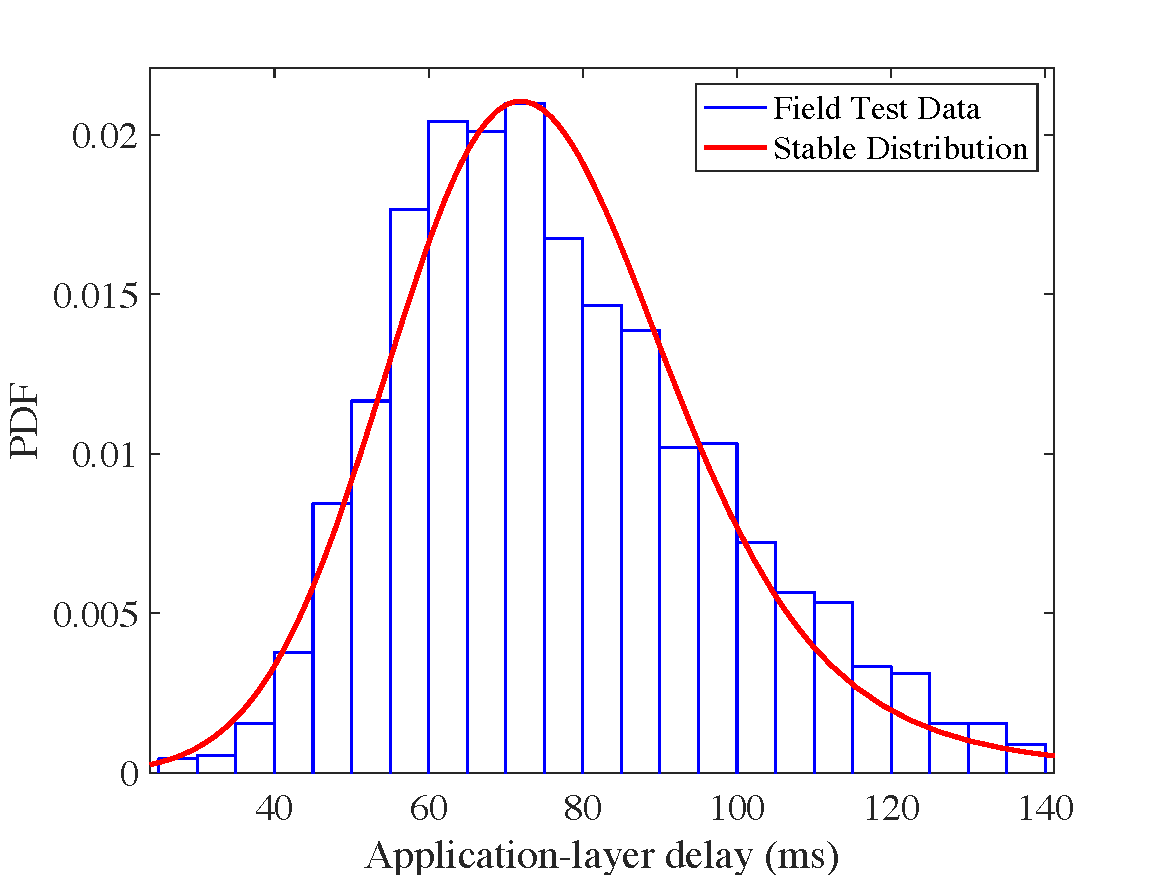
\includegraphics[width=0.8\columnwidth]{Fig5-3-delay-fitting.pdf}
  \bicaption{V2I应用层传输时延的概率密度函数}{Probability density function of application-layer V2I transmission delay}
  \label{fig 5-3}
\end{figure}

综上所述,给定观测数据集$X^{(0)}$,通过公式\ref{equ 5-10} 和公式\ref{equ 5-16},可以求解稳定分布的四个参数。
首先,给定观察数据集为$X^{(0)}=(x_1^{(0)}, x_2^{(0)}, \ldots, x_n^{(0)})$,在第$p$次迭代中,通过公式\ref{equ 5-18}对数据进行标准化。
\begin{equation}
x_{j}^{(p)}=\left(x_{j}^{(p-1)}-\mu_{p-1}\right) / \sigma_{p-1}, p = 1,2,\ldots
\label{equ 5-18}
\end{equation}
其中${\sigma_{0}=\left(x_{.72}-x_{.28}\right) / 1.654}$,$\mu_{0}$为25\%的截尾平均数,$x_{j}$是样本四分位数 \cite{fama1971parameter}。
本章选择最佳的$t_{k}=\pi k / 25, k=1,2,\ldots,K^{(p)}$\cite{koutrouvelis1980regression}来估计公式\ref{equ 5-10}中的$\hat{\alpha}^{(p)}$和$\hat{\sigma}^{(p)}$。
\begin{equation}
	{\hat{\alpha}^{(p)}=\frac{ \sum_{k=1}^{K^{(p)}} f\left(t_{k}\right)\left(\omega_{k}-\bar{\omega}\right)}{\sum_{k=1}^{K^{(p)}} \omega_{k}^{2}-\frac{1}{K}\left(\sum_{k=1}^{K^{(p)}} \omega_{k}\right)^{2}} } 
\end{equation}
\begin{equation}
	{\hat{\sigma}^{(p)}=\sqrt[\hat{\alpha}^{(p)}]{ (\exp \hat{b}^{(p)}) / 2}}
\end{equation}
其中 $f\left(t_{k}\right) = \ln \left(-\ln \left|\frac{1}{n} \sum_{j=1}^{n} \exp \left(i t_{k} x_{j}^{(p)}\right)\right|^{2}\right)$。

根据上述估计参数得到公式\ref{equ 5-16}中的另外两个估计参数$\hat{\beta}^{(p)}$和$\hat{\mu}^{(p)}$如公式\ref{equ 5-21}和\ref{equ 5-22}所示,其最佳$L^{p}$点为$t_{l}=\pi l / 25, l=1,2,\ldots,L^{(p)}$ \cite{koutrouvelis1980regression}。
\begin{equation}
\hat{\beta}^{(p)}= \frac{\hat{c}^{(p)}}{\bar{\sigma}^{\bar{\alpha}} \tan (\bar{\alpha} \pi / 2)}
\label{equ 5-21}
\end{equation}
\begin{equation}
\hat{\mu}^{(p)}= \frac{1}{L^{(p)}} \sum_{l=1}^{L^{(p)}}\left(\varphi\left(t_{l}\right)-\hat{c}^{(p)} d_{l}\right)
\label{equ 5-22}
\end{equation}
其中 $\bar{\alpha} =  {\hat{\alpha}^{(p)}}$ , $\bar{\sigma} =  {\hat{\sigma}^{(p)}}$,
\begin{equation}
\varphi\left(t_{l}\right) = \frac{1}{t_{l}} \arctan \left(\frac{ \sum_{j=1}^{n} \sin \left(t_l x_{j}^{(p)}\right)}{\sum_{j=1}^{n} \cos \left(t_l x_{j}^{(p)}\right)}\right)
\end{equation}

现场测试的1804个数据包传输时延被用于估计稳定分布模型,经过有限的迭代,得到了满足要求的四个估计参数。
图\ref{fig 5-3}显示了应用层时延的概率密度函数(Probability Density Function, PDF)。
结果显示,应用层时延分布几乎是对称的($\alpha = 1.77395$),并围绕平均值($\mu = 72.7343$)。
因此,有95\%的置信度,平均值的真值位于$71.9384$和$73.5301$的区间内。
可以看出,所得到的分布具有左偏度($\beta = 1$)且与均值的离散程度较大($\sigma = 13.3685$)。

\subsection{数据包丢失检测机制}

本章提出了一种基于历史信息的数据包丢失检测机制,其中历史信息包括数据传输频率和车辆位置。
首先,根据车辆的上传频率,边缘节点获取需要更新状态的车辆ID集合。
对于上传车辆集合中的车辆,如果边缘节点没有收到其上传的数据包,则可能存在以下两种情况:
第一,该车辆不在V2I通信范围内,导致数据包无法成功传递。
第二,该车辆在V2I通信范围内,但数据包在传输过程中丢失。
为了辨别这两种情况,在所提出的丢包检测机制中,边缘节点会根据历史位置判断车辆是否在通信范围内,如果在通信范围内却未收到相应数据包,则边缘节点认为该数据包已丢失。

不失一般性,本章考虑碰撞预警系统由单个边缘节点和若干辆车组成。
值得注意的是,该设置可直接扩展到多个边缘节点的情况。
在此场景中,集合$\mathbf{T}=\{1, \ldots, t, \ldots, T\}$表示离散时间片。
车辆集合用$\mathbf{V}=\{1, \ldots, v, \ldots, V\}$表示。
在时间 $t$,车辆 $v$ 的位置、速度、加速度分别用 $l_{v}^{t}$、$s_{v}^{t}$,以及$a_{v}^{t}$ 表示。
边缘节点用$e$表示,其位置用 ${l}_{e}$ 表示,且V2I通信范围用 $g_e$ 表示。
在时间 $t$, 车辆 $v$ 与边缘节点$e$之间的距离用 $\operatorname{dis}_{v, e}^{t}$ 表示。
如果 $\operatorname{dis}_{v, e}^{t} \leq g_e$,则车辆 ${v}$ 可以与边缘节点进行V2I通信。
在时间 $t$,边缘节点接收到若干个数据包,该数据包集合用 $\mathbf{M}_{t}=\{1, \ldots, m, \ldots, {M}_t\}$ 表示,其中 $m =(l_{v}^{t}, s_{v}^{t}, a_{v}^{t})$,$m \in \mathbf{M}_{t}$。
同时,边缘节点记录每个时间片接收到的数据包,即使用集合 ${\mathbf{H}_{t}} = \{\mathbf{M}_{t-{H}_{t}}, \ldots, \mathbf{M}_{t-2}, \mathbf{M}_{t-1}\}$ 来表示在时间 $t$的 历史记录,其中${H}_{t}$为历史记录信息的长度。
基于上述定义,本章所提的基于历史信息的数据包丢失检测机制分为以下两个步骤:

\textbf{1)记录:}
边缘节点维护车辆ID集合$\mathbf{ID}_{t}$以记录时间 $t$ 时V2I 通信覆盖范围内所有车辆。
$\mathbf{ID}_{t}$ 可通过上一时刻的值$\mathbf{ID}_{t-1}$进行初始化。 
当边缘节点在时间 $t$ 收到若干个数据包 $\mathbf{M}_{t}$ 时,对于 $m =(l_{v}^{t}, s_{v}^{t}, a_{v}^{t})$,${m} \in M_{t}$,如果边缘节点第一次收到车辆 $v$ 的数据包,即${v} \notin \mathbf{ID}_{t}$,则将 $v$ 加入 $\mathbf{ID}_{t}$,即$\mathbf{ID}_{t} = \mathbf{ID}_{t} \cup \{v\}$。
边缘节点搜索 $\mathbf{M}_{t}$ 并将所有车辆ID添加到集合 $\mathbf{ID}_{\mathbf{M}_{t}}$。

\textbf{2)检测:}
对于车辆 ${v} \in \mathbf{ID}_{t} \cup \mathbf{ID}_{\mathbf{M}_{t}}$,存在两种可能性:
(a)${v} \in \mathbf{ID}_{t} \setminus \mathbf{ID}_{\mathbf{M}_{t}}$,即车辆 $v$ 可以与边缘节点通信,但是边缘节点未收到它的数据包;
(b)${v} \in \mathbf{ID}_{t} \cap \mathbf{ID}_{\mathbf{M}_{t}}$,即车辆 $v$ 可以与边缘节点通信,并且边缘节点收到了它的数据包。
因此,对于(a),边缘节点搜索 ${\mathbf{H}_{t}}$ 获取车辆的最新位置 $l_v^t$。
边缘节点使用距离阈值 $\tau$ 和时间阈值 $\gamma$ 来检测车辆是否超出通信范围。
如果车辆 $v$ 与边缘节点$e$之间的距离 $\operatorname{dis}_{v, e}^{t} \geq g_e - \tau$,那么表示车辆 $v$ 正在离开通信范围,边缘节点将 $v$ 从 $\mathbf{ID}_{t}$ 中移除,即$\mathbf{ID}_{t}=\mathbf{ID}_{t} \setminus \{v\}$。
如果 $\operatorname{dis}_{v, e}^{t} < g_e - \tau$,则表示车辆 $v$ 可以与边缘节点通信,但是边缘节点未收到它的数据包。
预估的数据包接收时间为 $t_r$,如果 $t - t_r > \gamma$,则边缘节点认为数据包已丢失。
否则存在以下两种情况:车辆 $v$ 尚未发送数据包,或由于无线通信时延导致数据包暂未收到。

\subsection{工作流程}

本章节介绍基于视图修正的碰撞预警算法的具体流程,如算法5.1所示。
首先,基于V2I传输时延拟合模型估计数据包传输时延,并根据车辆速度和加速度更新其实时状态。
其次,检测丢失的数据包,并使用边缘节点中的历史记录更新它们的状态。
再次,使用模拟的传输时延来校准车辆轨迹以获得更加准确实时的逻辑视图。
进一步,基于修正的视图预测所有车辆未来的轨迹。
最后,通过计算每对车辆的车头时距并通过车头时距阈值来检测潜在碰撞。
VCCW具体步骤如下:

\SetKwInOut{KwIn}{输入}
\SetKwInOut{KwOut}{输出}

\begin{algorithm}[h]\small
\renewcommand{\algorithmcfname}{算法}
	\caption{基于视图修正的碰撞预警}
	\KwIn{车辆ID集合$\mathbf{ID}_{t}$、收到的数据包$\mathbf{M}_{t}$、历史记录${\mathbf{H}_{t}}$、车辆轨迹预测时间 $t_{\operatorname{pre}}$、碰撞预警距离阈值$\operatorname{dis}_{\operatorname{col}}$、车头时距阈值$\imath$}
	\KwOut{碰撞预警信息 $w_{v}^{t}$}
	初始化ID集合,$\mathbf{ID}_{t} = \mathbf{ID}_{t-1}$, $\mathbf{ID}_{\mathbf{M}_{t}} = \emptyset $ \\
	\For{$m \in \mathbf{M}_{t}$}{
		$\mathbf{ID}_{\mathbf{M}_{t}} =\mathbf{ID}_{\mathbf{M}_{t}} \cup \{v\}$\\
		\If{$v \notin \mathbf{ID}_{t}$}{
			$\mathbf{ID}_{t} = \mathbf{ID}_{t} \cup \{v\}$\\
		}
	}
	\For{$v \in \mathbf{ID}_{t} \cup \mathbf{ID}_{\mathbf{M}_{t}}$}{
		\If{$v \in \mathbf{ID}_{t} \setminus \mathbf{ID}_{\mathbf{M}_{t}}$}{
			搜索历史信息 ${\mathbf{H}_{t}}$ 并得到车辆最新数据包 $m$\\
			\If{$\operatorname{dis}_{v, e}^{t} \geq g_e - \tau$}{
				$\mathbf{ID}_{t} = \mathbf{ID}_{t} \setminus \{v\}$\\
			}
			\If{$\operatorname{dis}_{v, e}^{t} < g_e - \tau$ 且 $t - t_r > \gamma$}{
				$\mathbf{M}_{t} = \mathbf{M}_{t} \cup \{ m \}$\\
			}
		}
	}
	\For{$m \in \mathbf{M}_{t}$}{
		${t_{\operatorname{int}}} = t - {t_{r}} + t_{f}^v$,并通过公式\ref{equ 5-24}更新车辆位置\\
		\While{${t_{\operatorname{int}}} > t + t_{\operatorname{pre}}$}{
			$t = t + \frac{1}{\xi}$,并根据公式\ref{equ 5-24} 计算车辆位置 $l_v^{t}$ \\
			$\mathbf{Tra}_{v} = \mathbf{Tra}_{v} \cup \{ l_v^t \}$\\
		}
		$\mathbf{Tra} = \mathbf{Tra} \cup \{\mathbf{Tra}_{v}\}$
	}
	\For{$\mathbf{Tra}_{v} \in \mathbf{Tra}$ \songti{且} $\mathbf{Tra}_{v^{\prime}} \in \mathbf{Tra} \setminus \{ \mathbf{Tra}_{v}\}$}{
		\For{$l_v^t \in \mathbf{Tra}_{v}$ \songti{且} $l_{v^{\prime}}^{t^{\prime}} \in \mathbf{Tra}_{v^{\prime}}$}{
			\If{$\operatorname{dis}_{v, v^{\prime}}^{t, t^{\prime}} < \operatorname{dis}_{\operatorname{col}}$}{
				${h}_{v, v^{\prime}} = |t - t^{\prime}|$\\
				\If{${h}_{v, v^{\prime}} < \imath$}{
					$w_{v}^{t} = w_{v^{\prime}}^{t^{\prime}} = 1$\\
				}
			}
		}
	}
	\label{algorithm 5-1}
\end{algorithm}

\textbf{1)车辆ID集合更新:}
在时间 $t$ 初始化车辆ID集合 $\mathbf{ID}_{t}$ 和收到的数据包 $\mathbf{M}_{t}$ 的 ID集合 $\mathbf{ID}_{\mathbf{M}_{t}}$。
其中$\mathbf{ID}_{\mathbf{M}_{t}}$ 包含了接收数据包中的所有车辆ID。
如果车辆ID没有包含在 $\mathbf{ID}_{t}$ 中,则边缘节点将该车辆ID添加到 $\mathbf{ID}_{t}$ 中。

\textbf{2)数据包丢失检测:}
边缘节点通过数据包丢失检测机制得到数据包丢失的车辆集合,对于数据包丢失的车辆,边缘节点将在数据包历史记录${\mathbf{H}_{t}}$中搜索最新的车辆状态信息,并将其添加到$\mathbf{M}_{t}$中。

\textbf{3)基于车辆轨迹校准的视图修正:}
对于数据包$m \in \mathbf{M}_{t}$,边缘节点基于稳定分布生成符合V2I传输时延拟合模型的随机数来估计数据包的传输时延$t_{f}^v$。
在此基础上,边缘节点估计数据包的发送时间${\hat t_{c}} = {t_{r}} - t_{f}^v$。
时间$t$和数据包发送时间${\hat t_{c}}$之间的时间间隔为${t_{\operatorname{int}}} = t - {t_{r}} + t_{f}^v$。
进一步,边缘节点更新车辆$v$的位置信息。
\begin{numcases}{}
	{l_x}_v^t = {l_x}_v^{{\hat t_{c}}} + {t_{\operatorname{int}}} {s_x}_v^{{\hat t_{c}}} + \frac{{t_{\operatorname{int}}}^2 {a_x}_v^{{\hat t_{c}}}}{2} \notag \\
	{l_y}_v^t = {l_y}_v^{{\hat t_{c}}} + {t_{\operatorname{int}}} {s_y}_v^{{\hat t_{c}}} + \frac{{t_{\operatorname{int}}}^2 {a_y}_v^{{\hat t_{c}}}}{2}
\label{equ 5-24}
\end{numcases}
其中,${l_x}_v^{{\hat t_{c}}}$、${l_y}_v^{{\hat t_{c}}}$、${s_x}_v^{{\hat t_{c}}}$、${s_y}_v^{{\hat t_{c}}}$、${a_x}_v^{{\hat t_{c}}}$,以及${a_y}_v^{{\hat t_{c}}}$分别表示车辆$v$在X和Y坐标系中的位置、速度和加速度。

\textbf{4)车辆未来轨迹预测:}
对于车辆$v$,边缘节点在时间段$(t, t + t_{\operatorname{pre}})$内预测其未来轨迹,其中$t_{\operatorname{pre}}$是车辆轨迹预测时间。
边缘节点每隔$\frac{1}{\xi}$秒计算一次车辆位置,其中$\xi$为车辆位置更新频率,并将计算得到的新位置添加到车辆$v$轨迹集合$\mathbf{Tra}_{v}$中。

\textbf{5)潜在碰撞检测:}
碰撞预警预警信息集合用 $\mathbf{W}_t = \{ 1, \ldots, w_{v}^{t}, \ldots, W_t\}$ 表示,其中 $w_{v}^{t}$ 是一个0-1变量,表示车辆$v$是否有潜在碰撞风险。
对于位置信息满足$l_v^t \in \mathbf{Tra}_{v}$ 且 $l_{v^{\prime}}^{t^{\prime}} \in \mathbf{Tra}_{v^{\prime}}$ 的车辆对,边缘节点计算两辆车的距离$\operatorname{dis}_{v, v^{\prime}}^{t, t^{\prime}}$。
如果$\operatorname{dis}_{v, v^{\prime}}^{t, t^{\prime}} < \operatorname{dis}_{\operatorname{col}}$,其中$\operatorname{dis}_{\operatorname{col}}$为碰撞预警距离阈值, 则假定车辆$v$和$v^{\prime}$经过同一点。
前车的车头通过道路上的某一点和后车的车头通过同一点之间的时间被定义为车头时距\cite{vogel2003comparison}。
因此,边缘节点计算两车间的车头时距 ${h}_{v, v^{\prime}} = |t - t^{\prime}|$,如果${h}_{v, v^{\prime}} < \imath$,其中$\imath$是车头时距阈值,碰撞预警信息将被触发,即$w_{v}^{t} = w_{v^{\prime}}^{t^{\prime}} = 1$。

\section{实验结果与分析}\label{section 5-4}

\subsection{实验设置}

首先,本章在仿真实验中使用了收集自德国科隆市约400平方公里区域约120万辆真实出租车轨迹的数据集\cite{uppoor2013generation}。
本章选取了5个具有不同交通特征的路口来进行碰撞预警仿真实验,不同场景的具体交通特征如表\ref{table 6-1}所示。
场景1、2和3中,实验开始时间分别为晚上10点、早上8点和晚上7点。
在场景4和5中,实验开始时间为下午4点和6点。
边缘节点安装在前三个场景的$(10422.0, 12465.3)$和最后两个场景的$(6097.1, 14870.0)$处。
每个实验的持续时间为100 s,V2I通信范围设置为500 m。

\begin{table}[h]\small
\centering
\bicaption{不同场景的交通特征}{Traffic characteristics of different scenarios}
\setlength{\tabcolsep}{9.5mm}{
\begin{tabular}{cccc}
\toprule
场景&车辆数量&平均速度 (km/h)&平均加速度 (m/s$^2$)\\
\midrule
1& 54& 50.44& 0.203\\
2& 81& 46.58& 0.007\\
3& 106& 38.1& 0.075\\
4& 85& 69.19& 0.165\\
5& 114& 69.05& 0.060\\
\bottomrule
\end{tabular}}
\label{table 6-1}
\end{table}

为了进一步比较所提算法的性能,本章实现了两种具有对比性的碰撞检测算法。
\begin{itemize}
	\item \textbf{基于云的碰撞预警}:其是在集中式的云计算架构中实现的。具体地,车辆将其状态信息上传到距离车辆较远的云服务器。在仿真实验中,使用现场测试实验获得的V2C传输时延来模拟车辆和云节点之间的通信时延。云服务器没有对视图进行修正,仅基于车辆状态预测潜在碰撞。
	\item \textbf{基于边缘的碰撞预警}:其实现在车载边缘计算架构中。具体地,车辆将其状态上传到附近的边缘服务器,并使用在真实世界场地测试中获得的V2I传输时延来模拟车辆和边缘服务器之间的通信时延。与基于云的碰撞预警类似,边缘节点在没有对视图进行修正的情况下预测潜在碰撞。
\end{itemize}

为了进一步评估所提算法的性能,本章首先定义以下指标:
系统预测的碰撞预警消息集合用$\mathbf{W}_{p}$表示,$\left| \mathbf{W}_{p} \right|$是碰撞预警系统给出的潜在碰撞预警数量。
实验设置期望的碰撞预警集合用$\mathbf{W}_{d}$表示,$\left| \mathbf{W}_{d} \right|$为实验设置的实际发生碰撞的数量。
进一步,$\left| \mathbf{W}_{d} \cap \mathbf{W}_{p} \right|$表示碰撞预警系统成功预测的数量。
$\left| \mathbf{W}_{d} - \mathbf{W}_{p} \right|$是应该被触发但未被碰撞预警系统成功预测的预期预警数量,换言之,其表示$\mathbf{W}_{p}$中的预测失败的数量。
同样地,$\left| {\mathbf{W}_{p} - \mathbf{W}_{d}} \right|$表示碰撞预警系统错误预测的数量。
因此,定义查准率(Precision)和查全率(Recall)如下
\begin{equation}
	\operatorname{Precision} = \frac{{\left| {\mathbf{W}_{d} \cap \mathbf{W}_{p}} \right|}}{{\left| {\mathbf{W}_{d} \cap \mathbf{W}_{p}} \right| + \left| {\mathbf{W}_{p} - \mathbf{W}_{d}} \right|}} = \frac{{\left| {\mathbf{W}_{d} \cap \mathbf{W}_{p}} \right|}}{\left| \mathbf{W}_{p} \right|}
\end{equation}
\begin{equation}
	\operatorname{Recall} = \frac{{\left| {\mathbf{W}_{d} \cap \mathbf{W}_{p}} \right|}}{{\left| {\mathbf{W}_{d} \cap \mathbf{W}_{p}} \right| + \left| {\mathbf{W}_{d} - \mathbf{W}_{p}} \right|}} = \frac{{\left| {\mathbf{W}_{d} \cap \mathbf{W}_{p}} \right|}}{\left| \mathbf{W}_{d} \right|} 
\end{equation}
其中,查准率代表被成功预测为发生碰撞的样本数占所有被预测为发生碰撞的样本数的比例,其衡量的是碰撞预警系统预测的碰撞预警中有多少是真正需要进行预警。
而查全率表示被成功预测为发生碰撞的样本数占所有实际发生碰撞的样本数的比例,其衡量的是碰撞预警系统能够成功预警多少个真正需要预警的碰撞。
显然,查准率与查全率是一对具有冲突的指标,因此,使用F1值(F1 Score)来进一步评估碰撞预警系统的性能,其为查准率和查全率的调和平均数,其定义如下:
\begin{equation}
	\operatorname{F1\ Score} = \frac{2 \cdot \operatorname{Precision} \cdot \operatorname{Recall}}{\operatorname{Precision} + \operatorname{Recall}} 
\end{equation}
其可进一步评估碰撞预警系统在查准率和查全率方面的均衡。

\subsection{实验结果与分析}

\begin{figure}[h]
     \centering
     \subfloat[][]{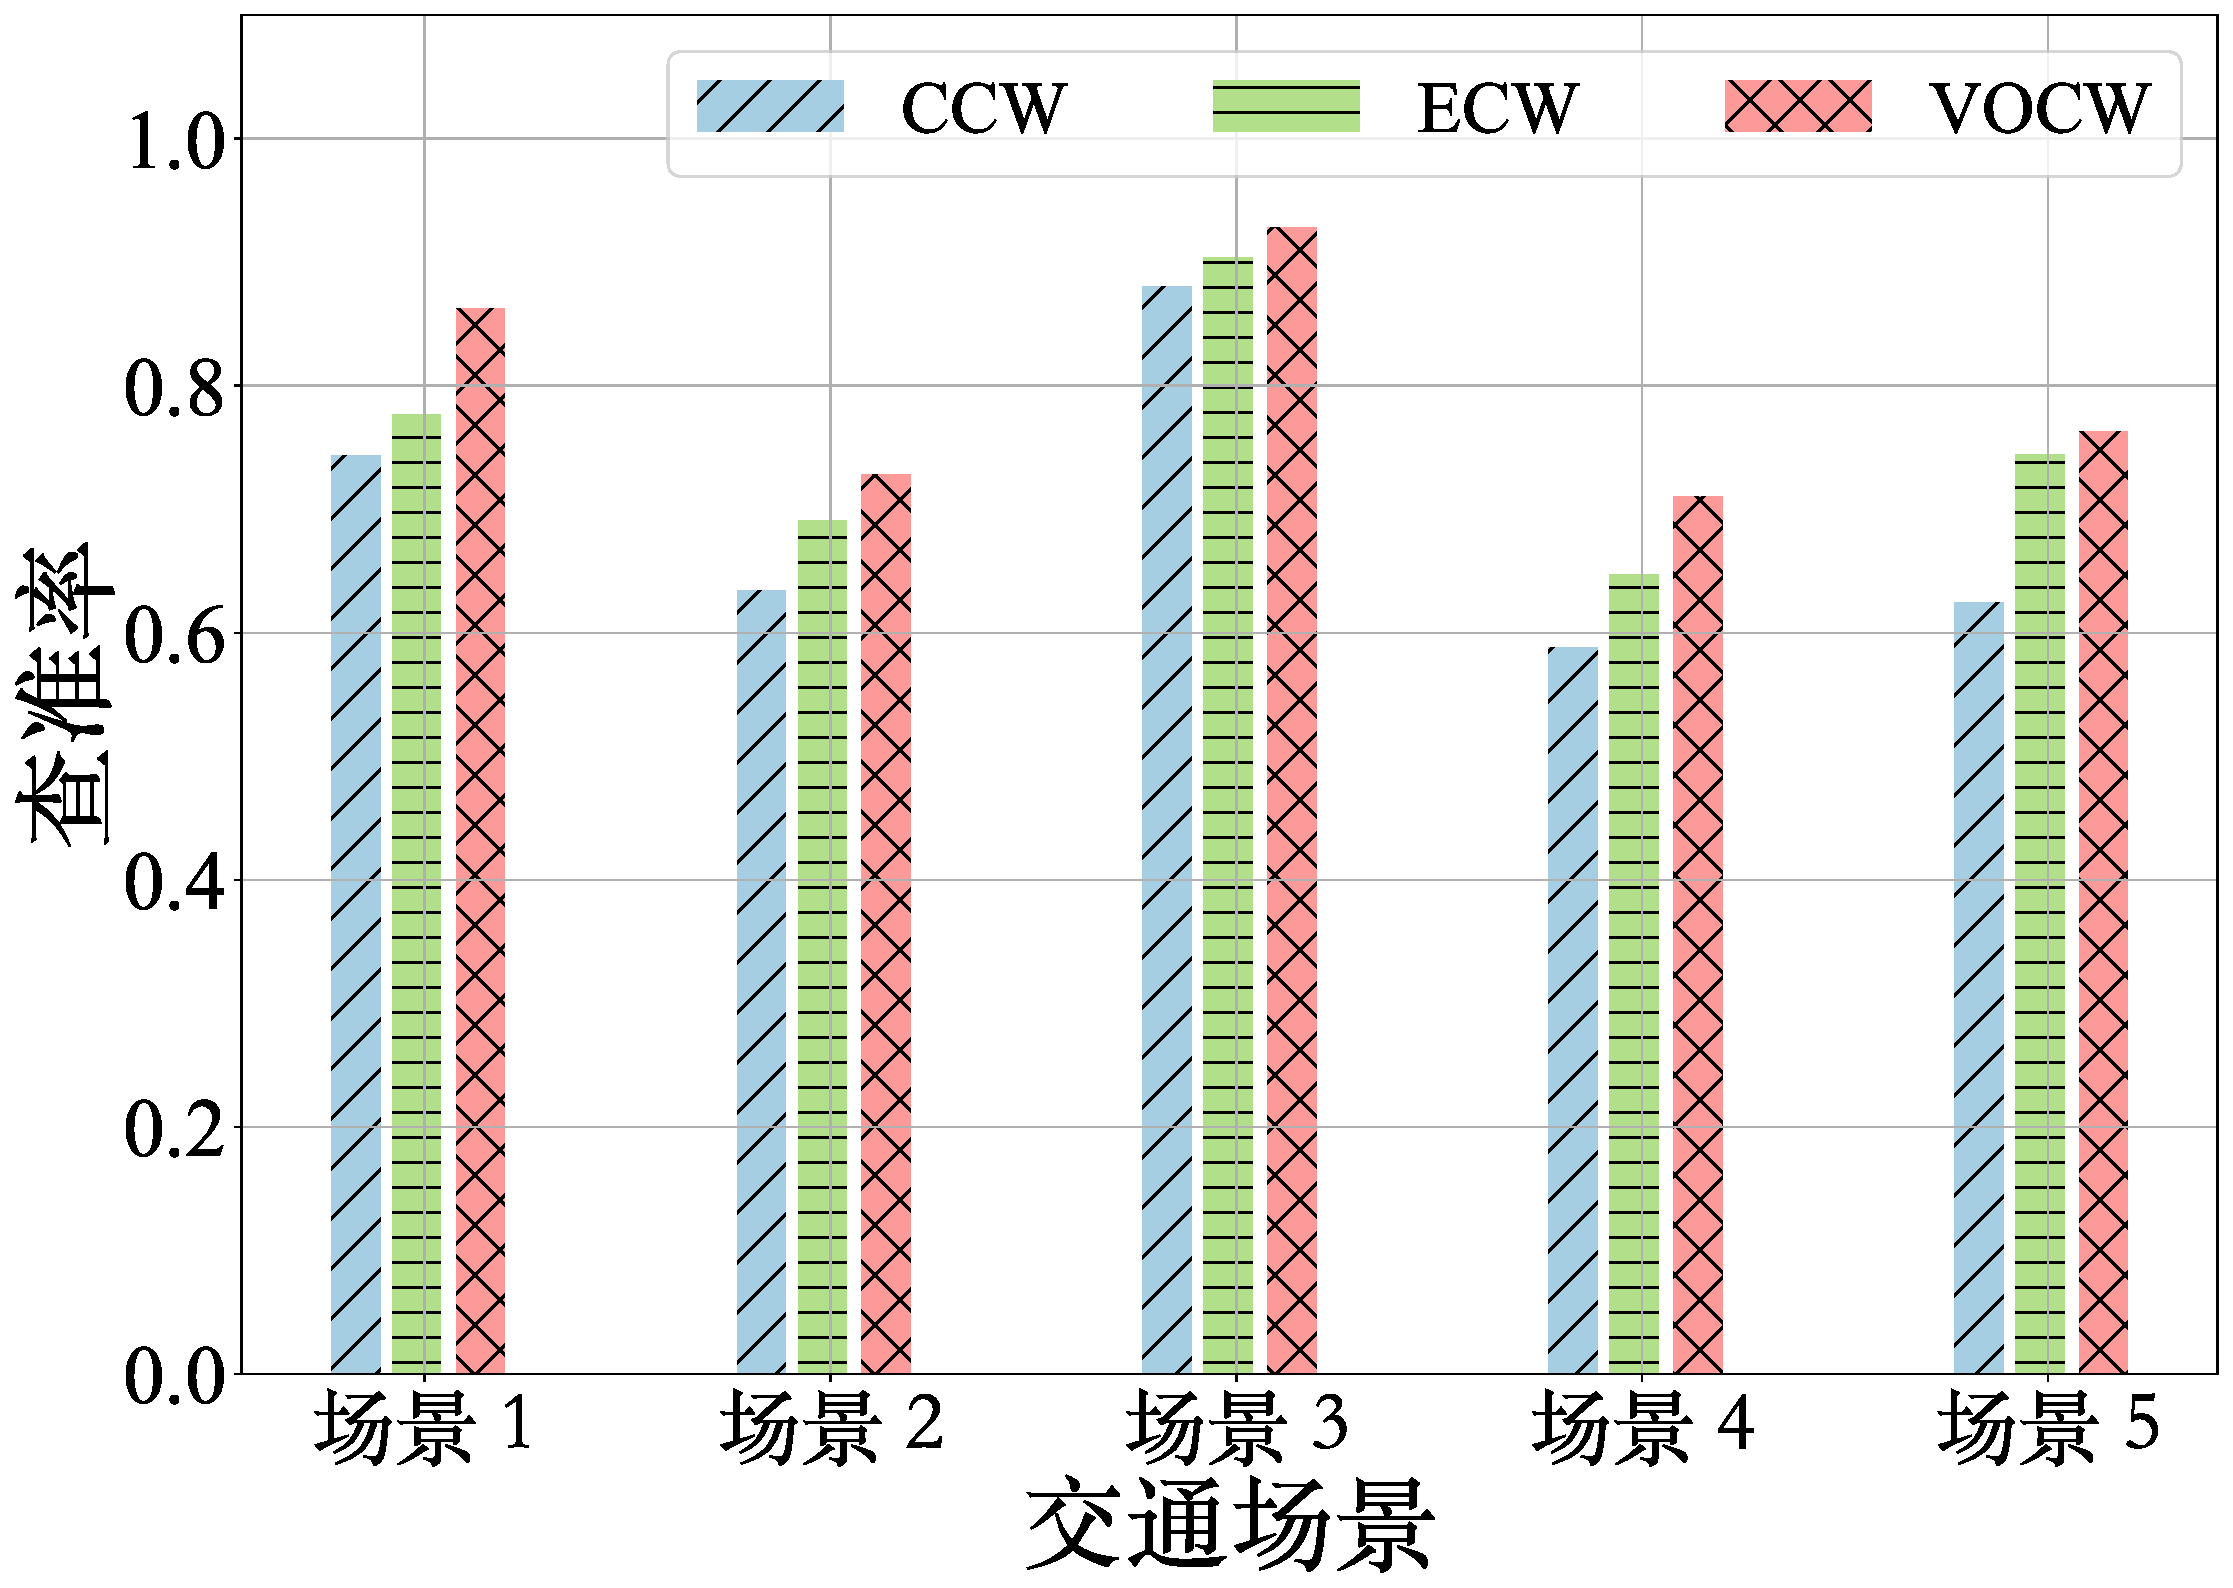
\includegraphics[width=0.33\columnwidth]{Fig5-5a-different-scenarios.pdf}}
     \subfloat[][]{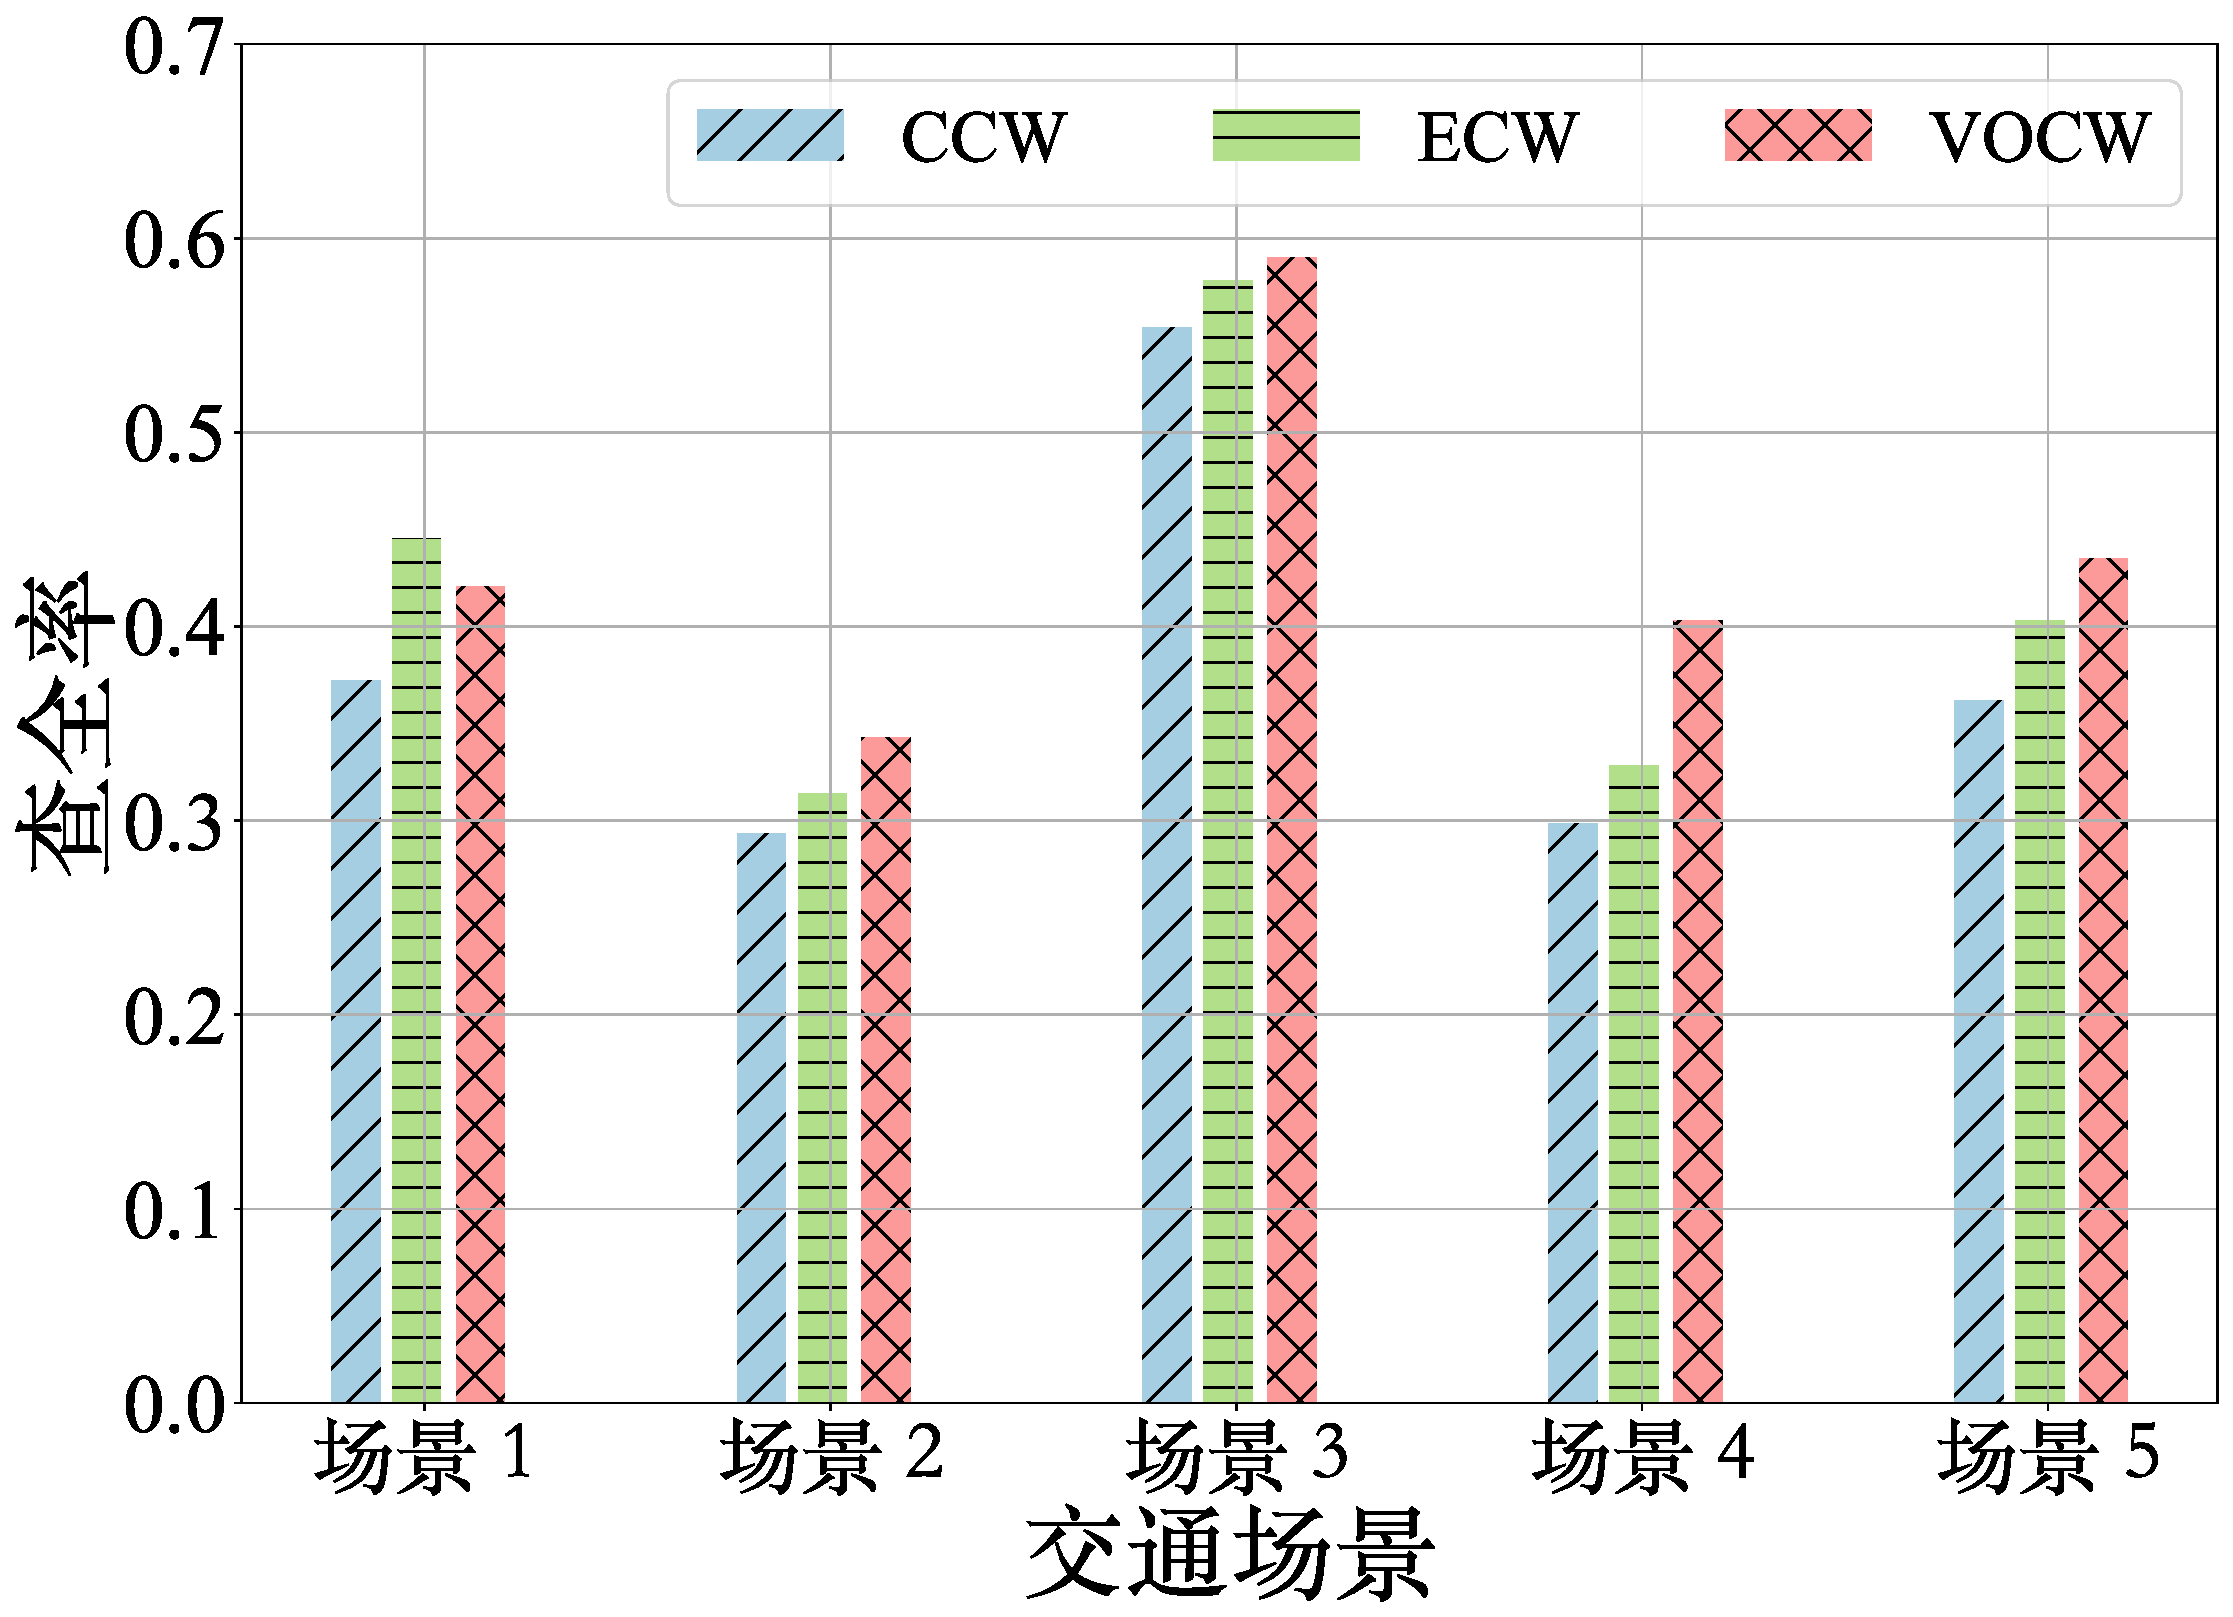
\includegraphics[width=0.33\columnwidth]{Fig5-5b-different-scenarios.pdf}}
     \subfloat[][]{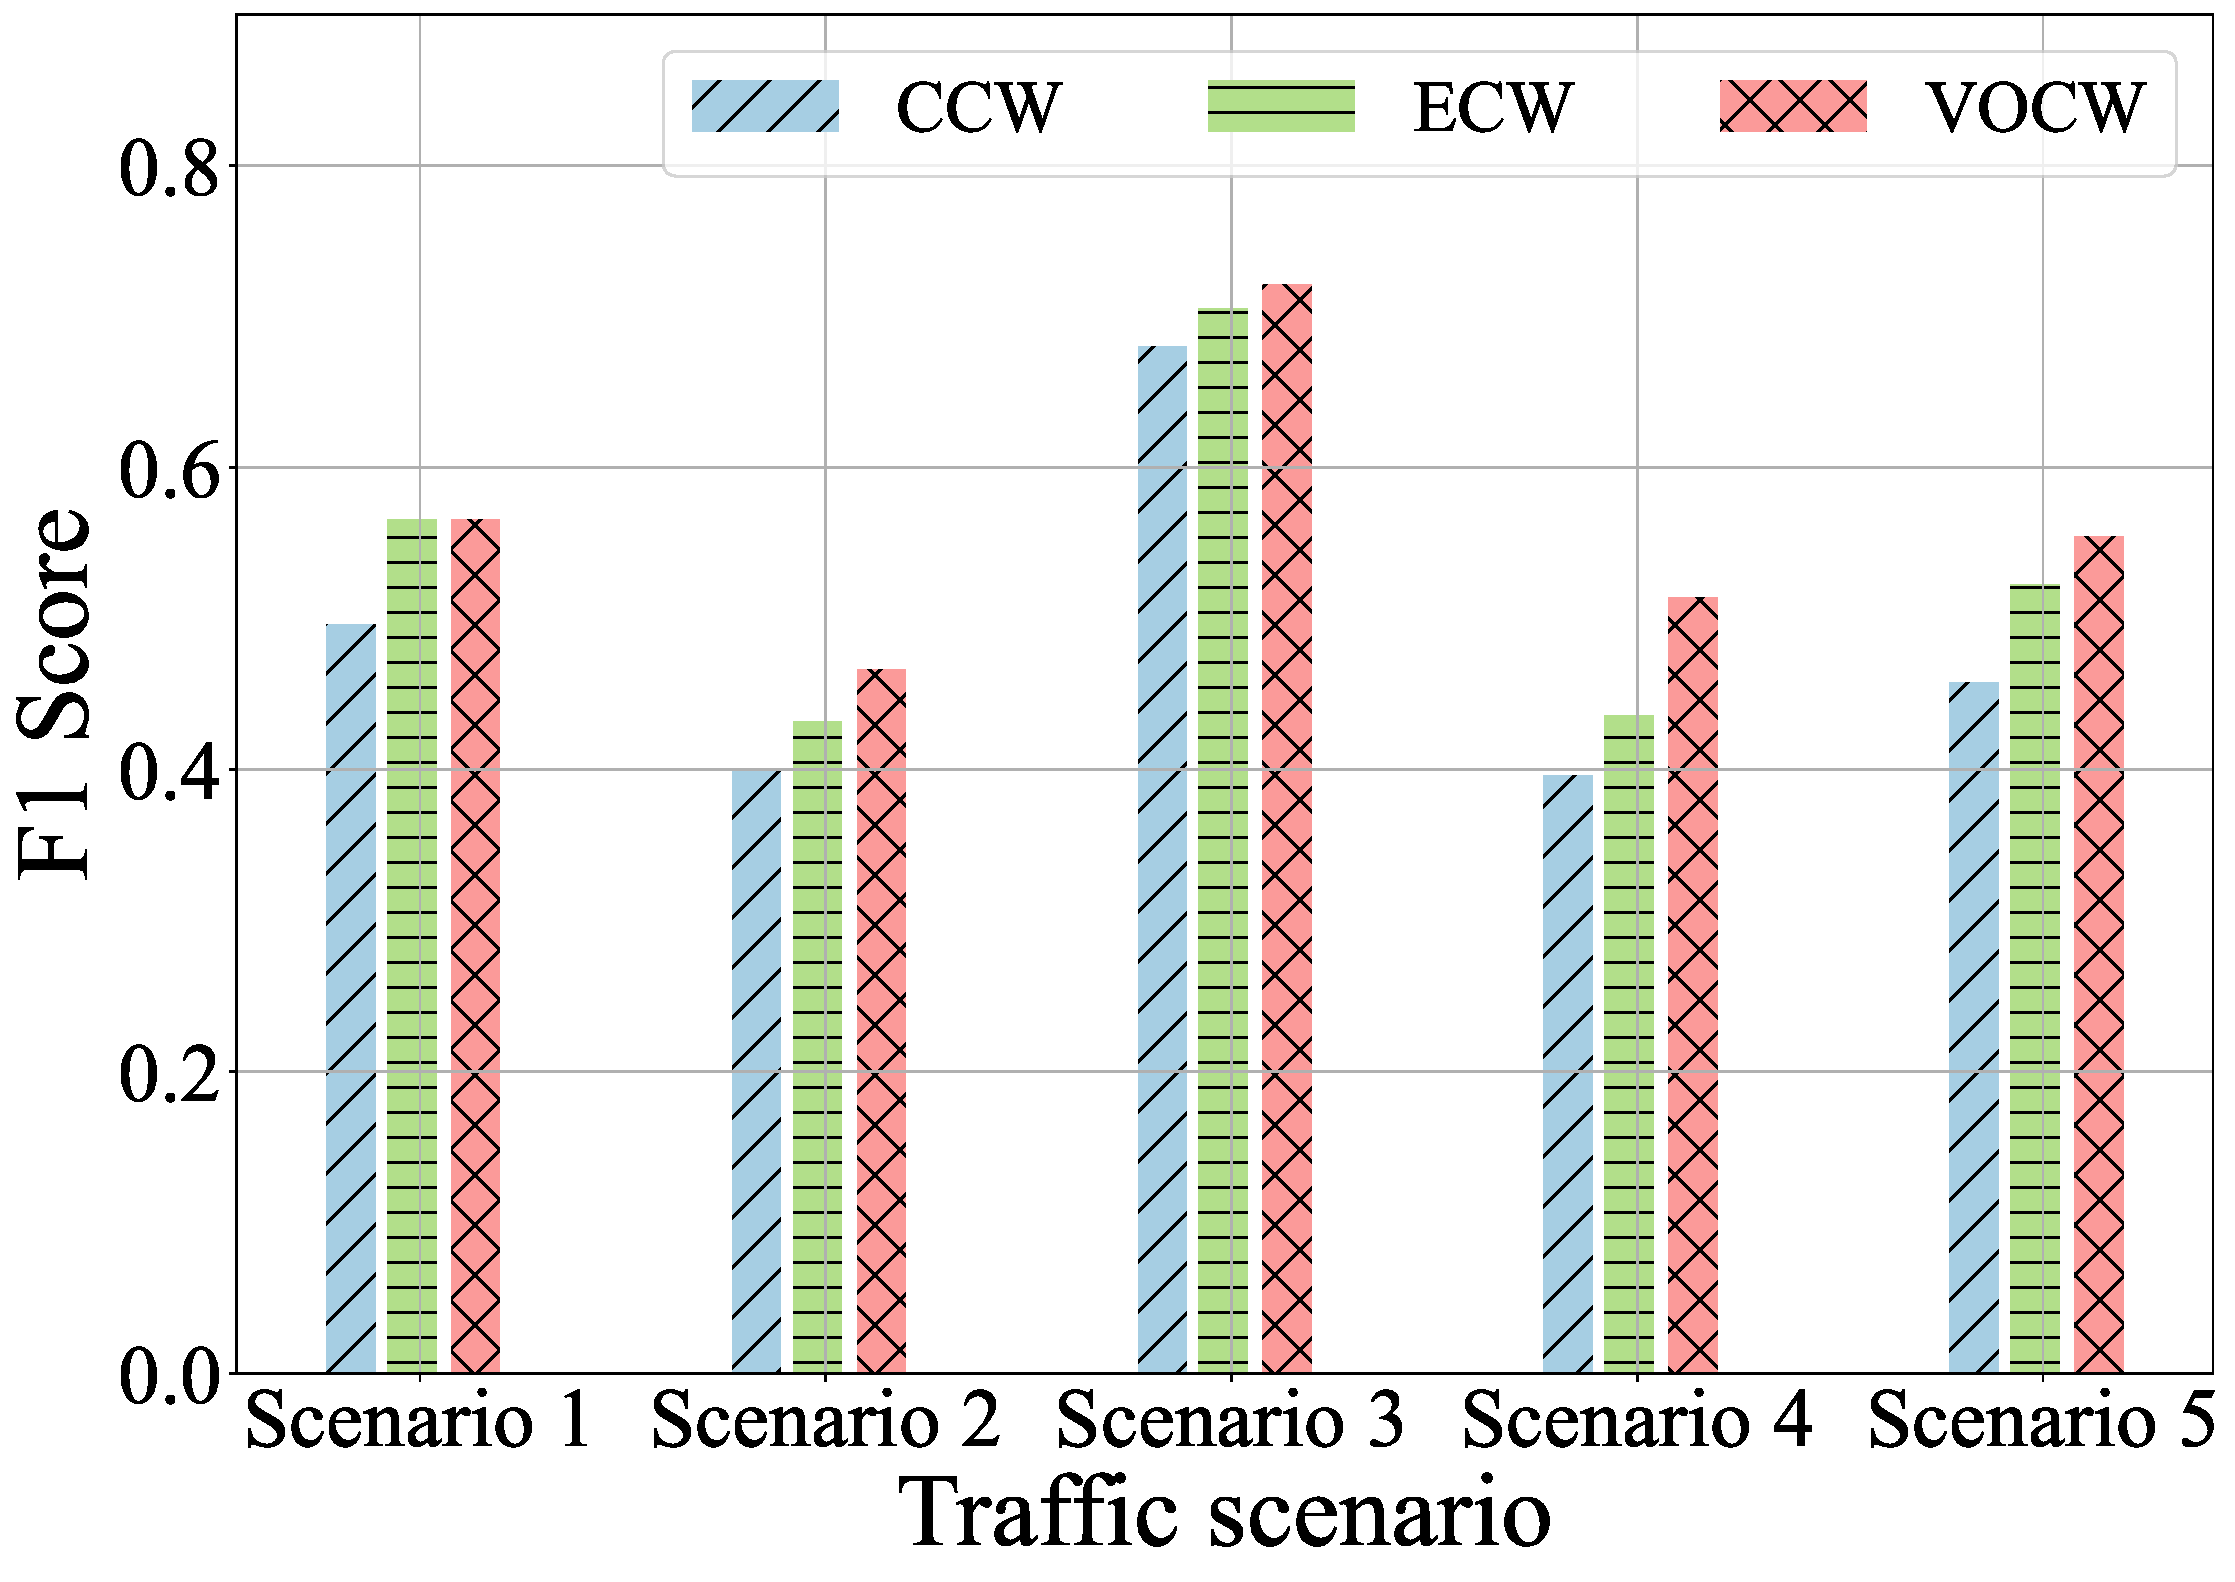
\includegraphics[width=0.33\columnwidth]{Fig5-5c-different-scenarios.pdf}}
     \bicaption[不同交通场景下的性能对比]{不同交通场景下的性能对比,其中不场景的交通特征列于表\ref{table 6-1}中。(a)查准率(b)查全率(c)F1值}[Performance comparison under different scenarios]{Performance comparison under different scenarios, the traffic characteristics of which are listed in Table. \ref{table 6-1}. (a) Precision (b) Recall (c) F1 score}
     \label{fig 5-4}
\end{figure}

\textbf{1) 不同交通场景的影响:}
图 \ref{fig 5-4} 比较了五个具有不同交通特征的场景中三种算法的性能。图 \ref{fig 5-4}(a)比较了三种算法的查准率。结果显示,VCCW在所有场景下的查准率最高。这是由于VCCW对边缘视图进行了修正,从而车辆状态更接近实时状态。因此,基于修正视图的碰撞预警可以提供更准确的服务。同样的结论也可以从图\ref{fig 5-4}(b)中得到,比较了三种算法的查全率。图\ref{fig 5-4}(c)比较了三种算法的F1值。结果表明,在所有交通场景下,VCCW都可以实现最高的F1值。

\textbf{2) 不同车头时距阈值的影响:}
图\ref{fig 5-5}比较了三种算法在不同车头时距阈值下的性能。其中,车头时距阈值从1秒增加至5秒。图\ref{fig 5-5}(a)比较了三种算法的查准率。可以看出,VCCW在不同车头时距阈值下都取得了最高的查准率。随着车头时距阈值的增加,查准率逐渐提高。这是因为随着车头时距阈值的增加,预测的碰撞预警数量也随之增加。因此,预测成功在整体预测数量中的比例也随之增加。图\ref{fig 5-5}(b)比较了三种算法的查全率。同样地,随着车头时距阈值的增加,查全率逐渐降低。图\ref{fig 5-5}(c)比较了三种算法的F1值。结果显示,与CCW和ECW相比,VCCW实现了最高的F1值。需要注意的是,ECW的性能明显高于CCW,这是因为ECW可以利用分布式车载边缘计算架构带来的更低的数据包传输时延,使得边缘构建的视图与云端构建的视图相比更加实时。

\begin{figure}[h]
     \centering
     \subfloat[][]{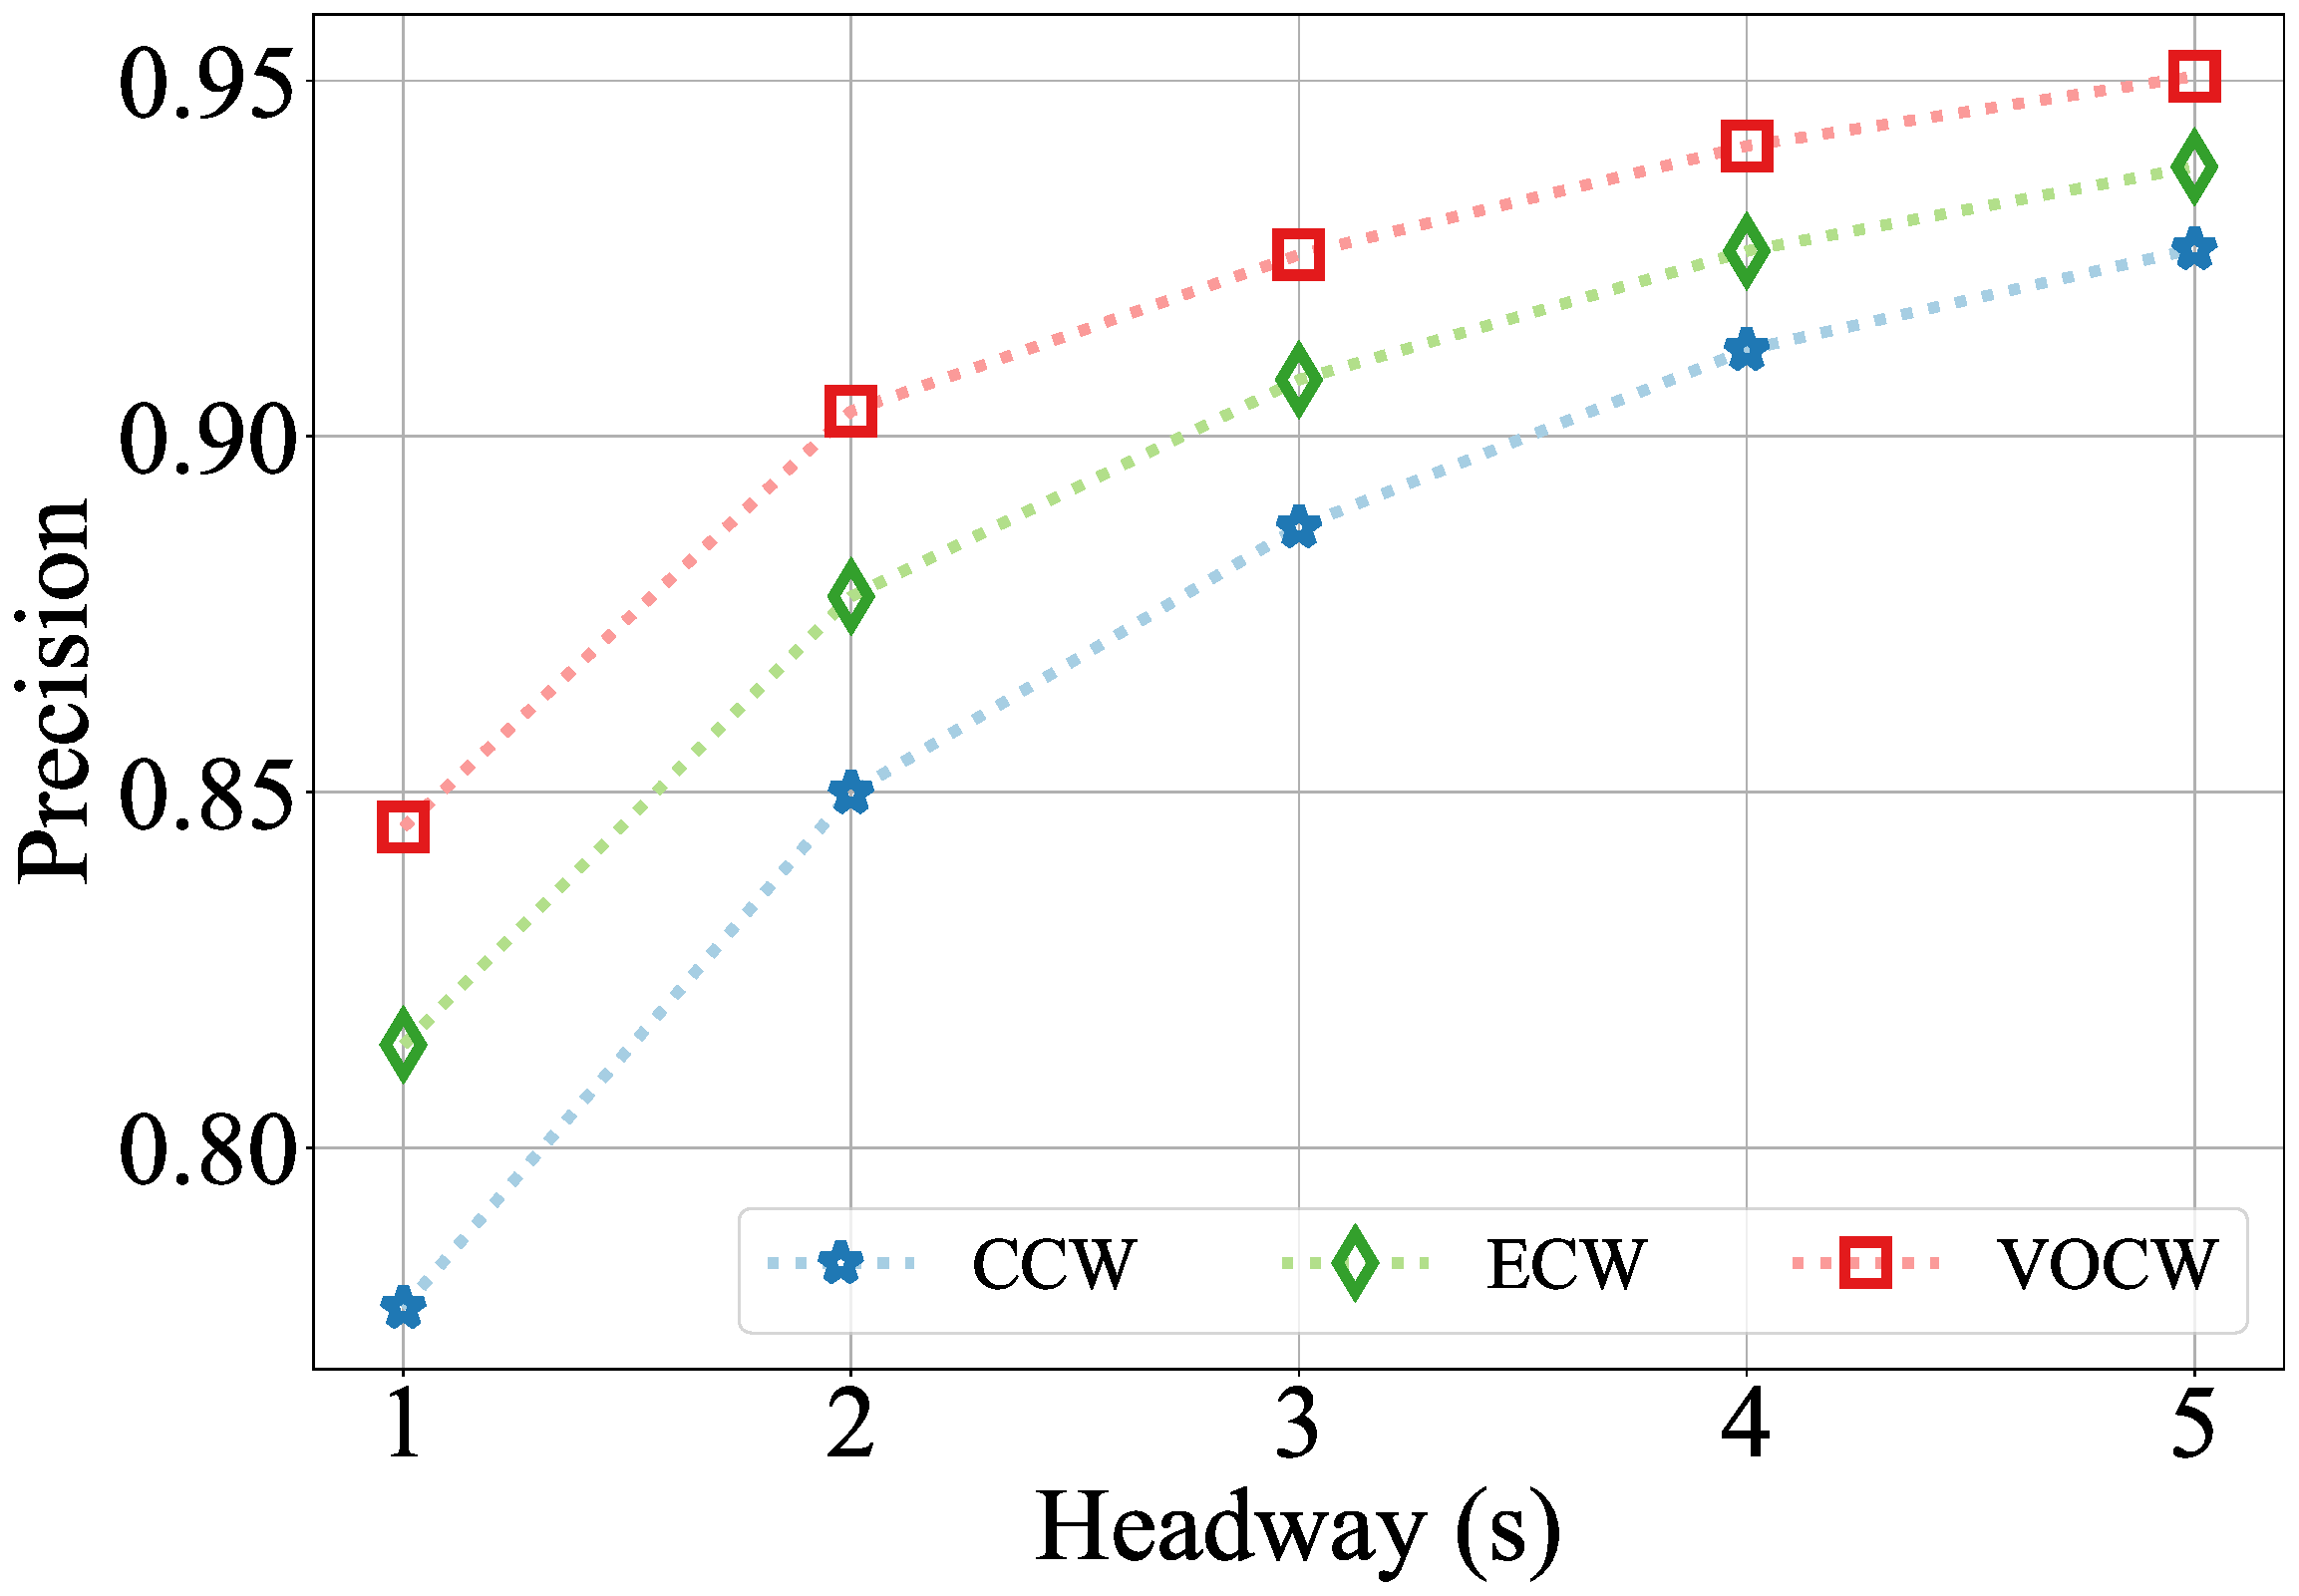
\includegraphics[width=0.33\columnwidth]{Fig5-6a-different-headways.pdf}}
     \subfloat[][]{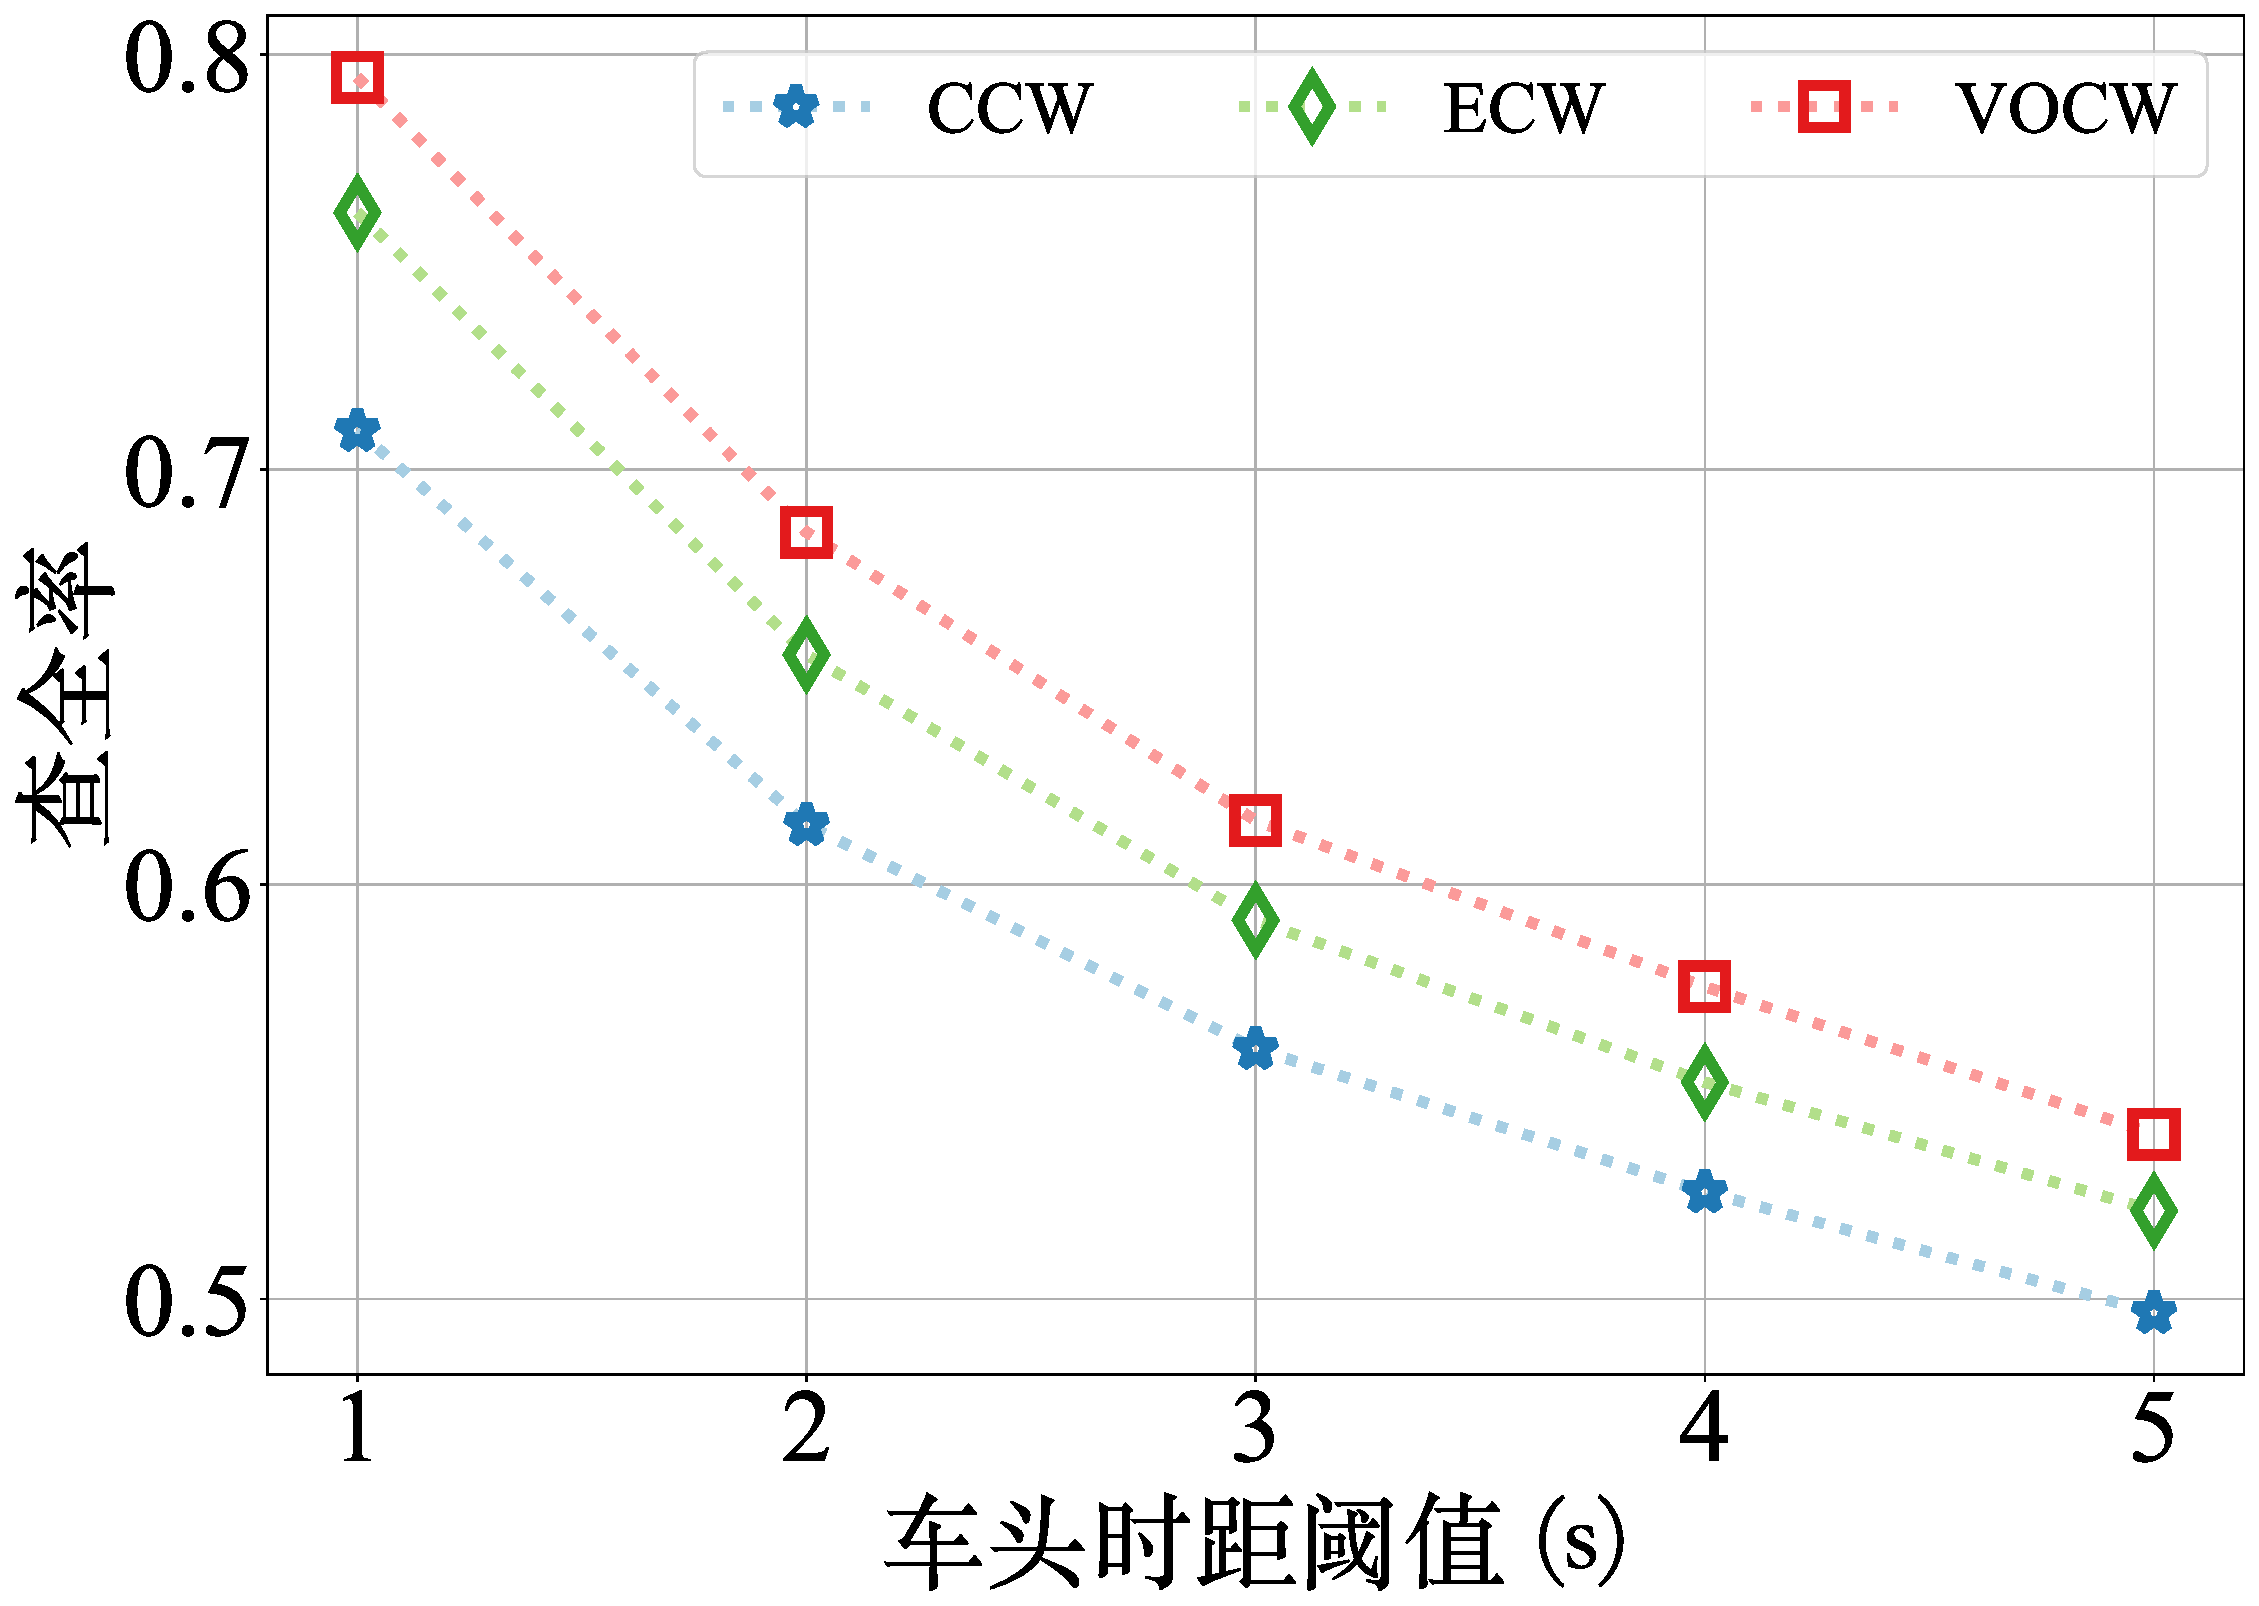
\includegraphics[width=0.33\columnwidth]{Fig5-6b-different-headways.pdf}}
     \subfloat[][]{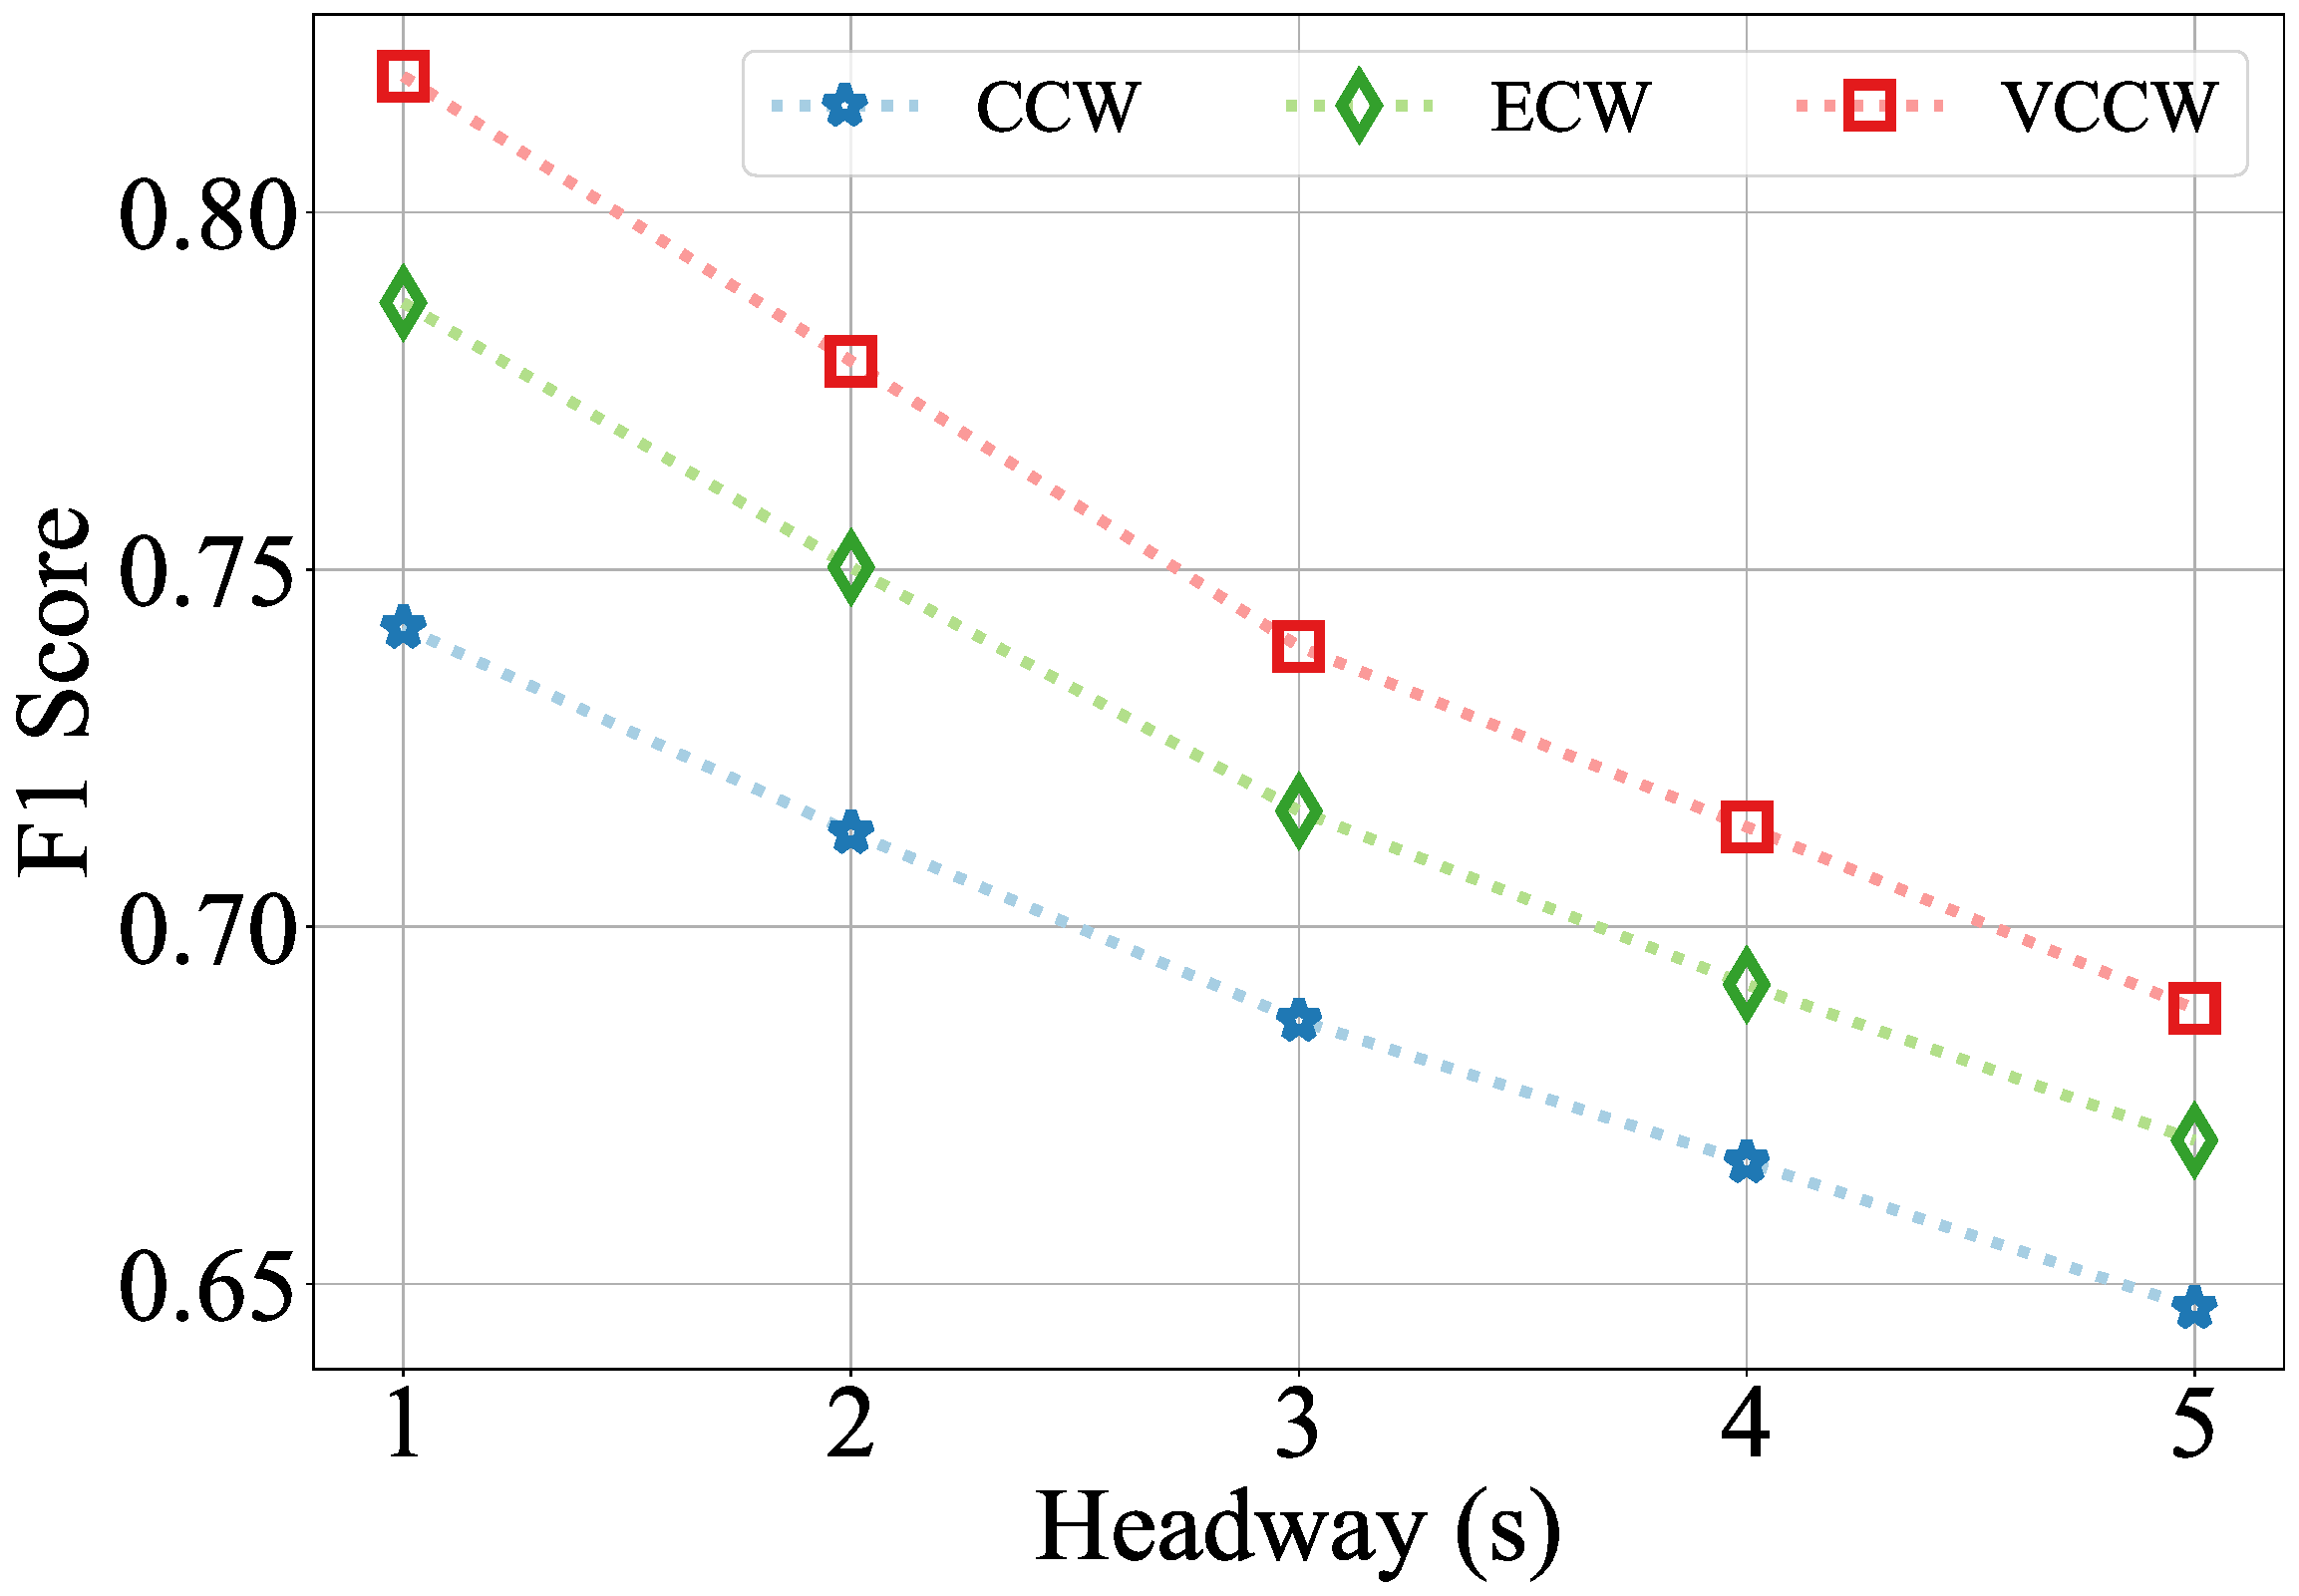
\includegraphics[width=0.33\columnwidth]{Fig5-6c-different-headways.pdf}}
     \bicaption[不同车头时距阈值下的性能对比]{不同车头时距阈值下的性能对比,其中车头时距阈值从1s 增加至 5s。(a)查准率(b)查全率(c)F1值}[Performance comparison under different headways]{Performance comparison under different headways, which increases from 1 to 5 s. (a) Precision (b) Recall (c) F1 score}
     \label{fig 5-5}
\end{figure}

\textbf{3) 不同丢包率的影响:}
图\ref{fig 5-6} 比较了三种算法在不同丢包率下的性能,丢包率从0\%增加至6\%。值得注意的是,随着丢包率的增加,所有算法的查全率均下降。这主要是因为随着丢包率的增加,边缘节点或云端仅能接收到不完整的车辆状态信息,因此碰撞预警系统将更难成功预测所有潜在碰撞风险。图\ref{fig 5-6}(a)、图\ref{fig 5-6}(b)和图\ref{fig 5-6}(c)分别比较了三种算法的查准率、查全率和F1值。结果表明,VCCW在所有情况下实现了最高的查准率、查全率和F1值。同时,CCW和ECW的性能明显比VCCW更差,这是因为它们都没有实现对视图的修正,因此无线传输中的丢包对它们的影响更大。

\begin{figure}[h]
     \centering
     \subfloat[][]{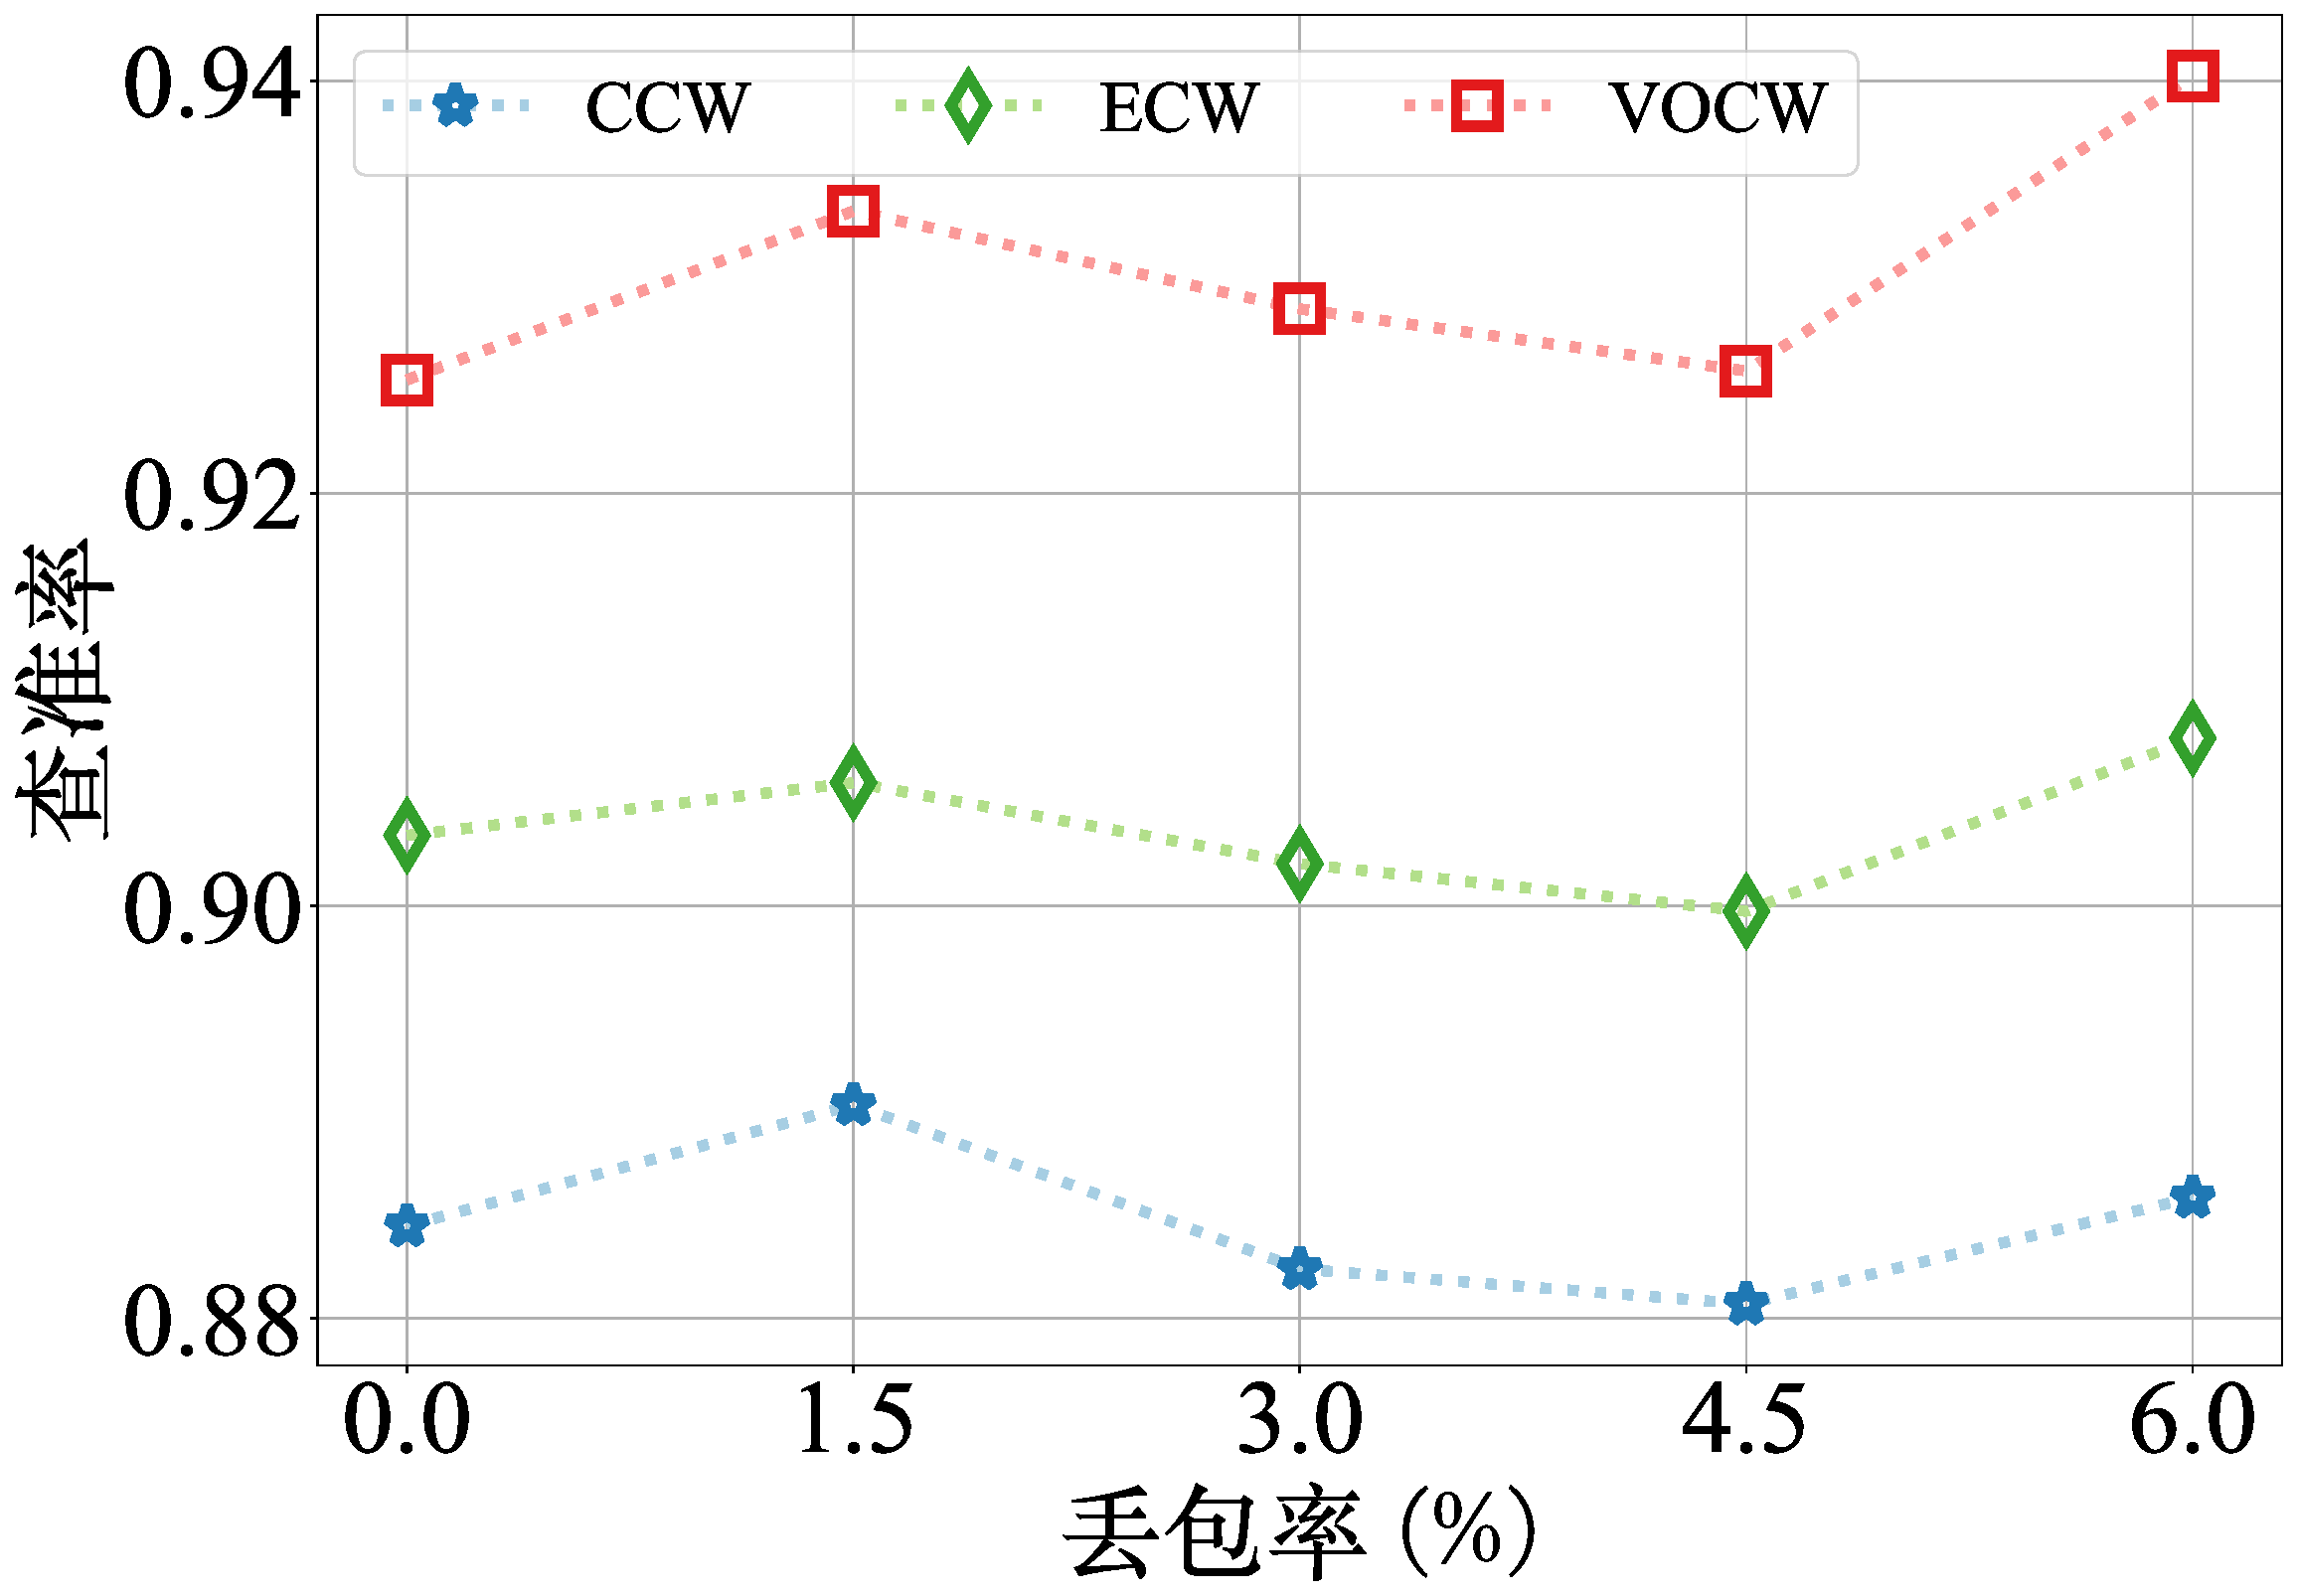
\includegraphics[width=0.33\columnwidth]{Fig5-7a-different-packet-loss-rate.pdf}}
     \subfloat[][]{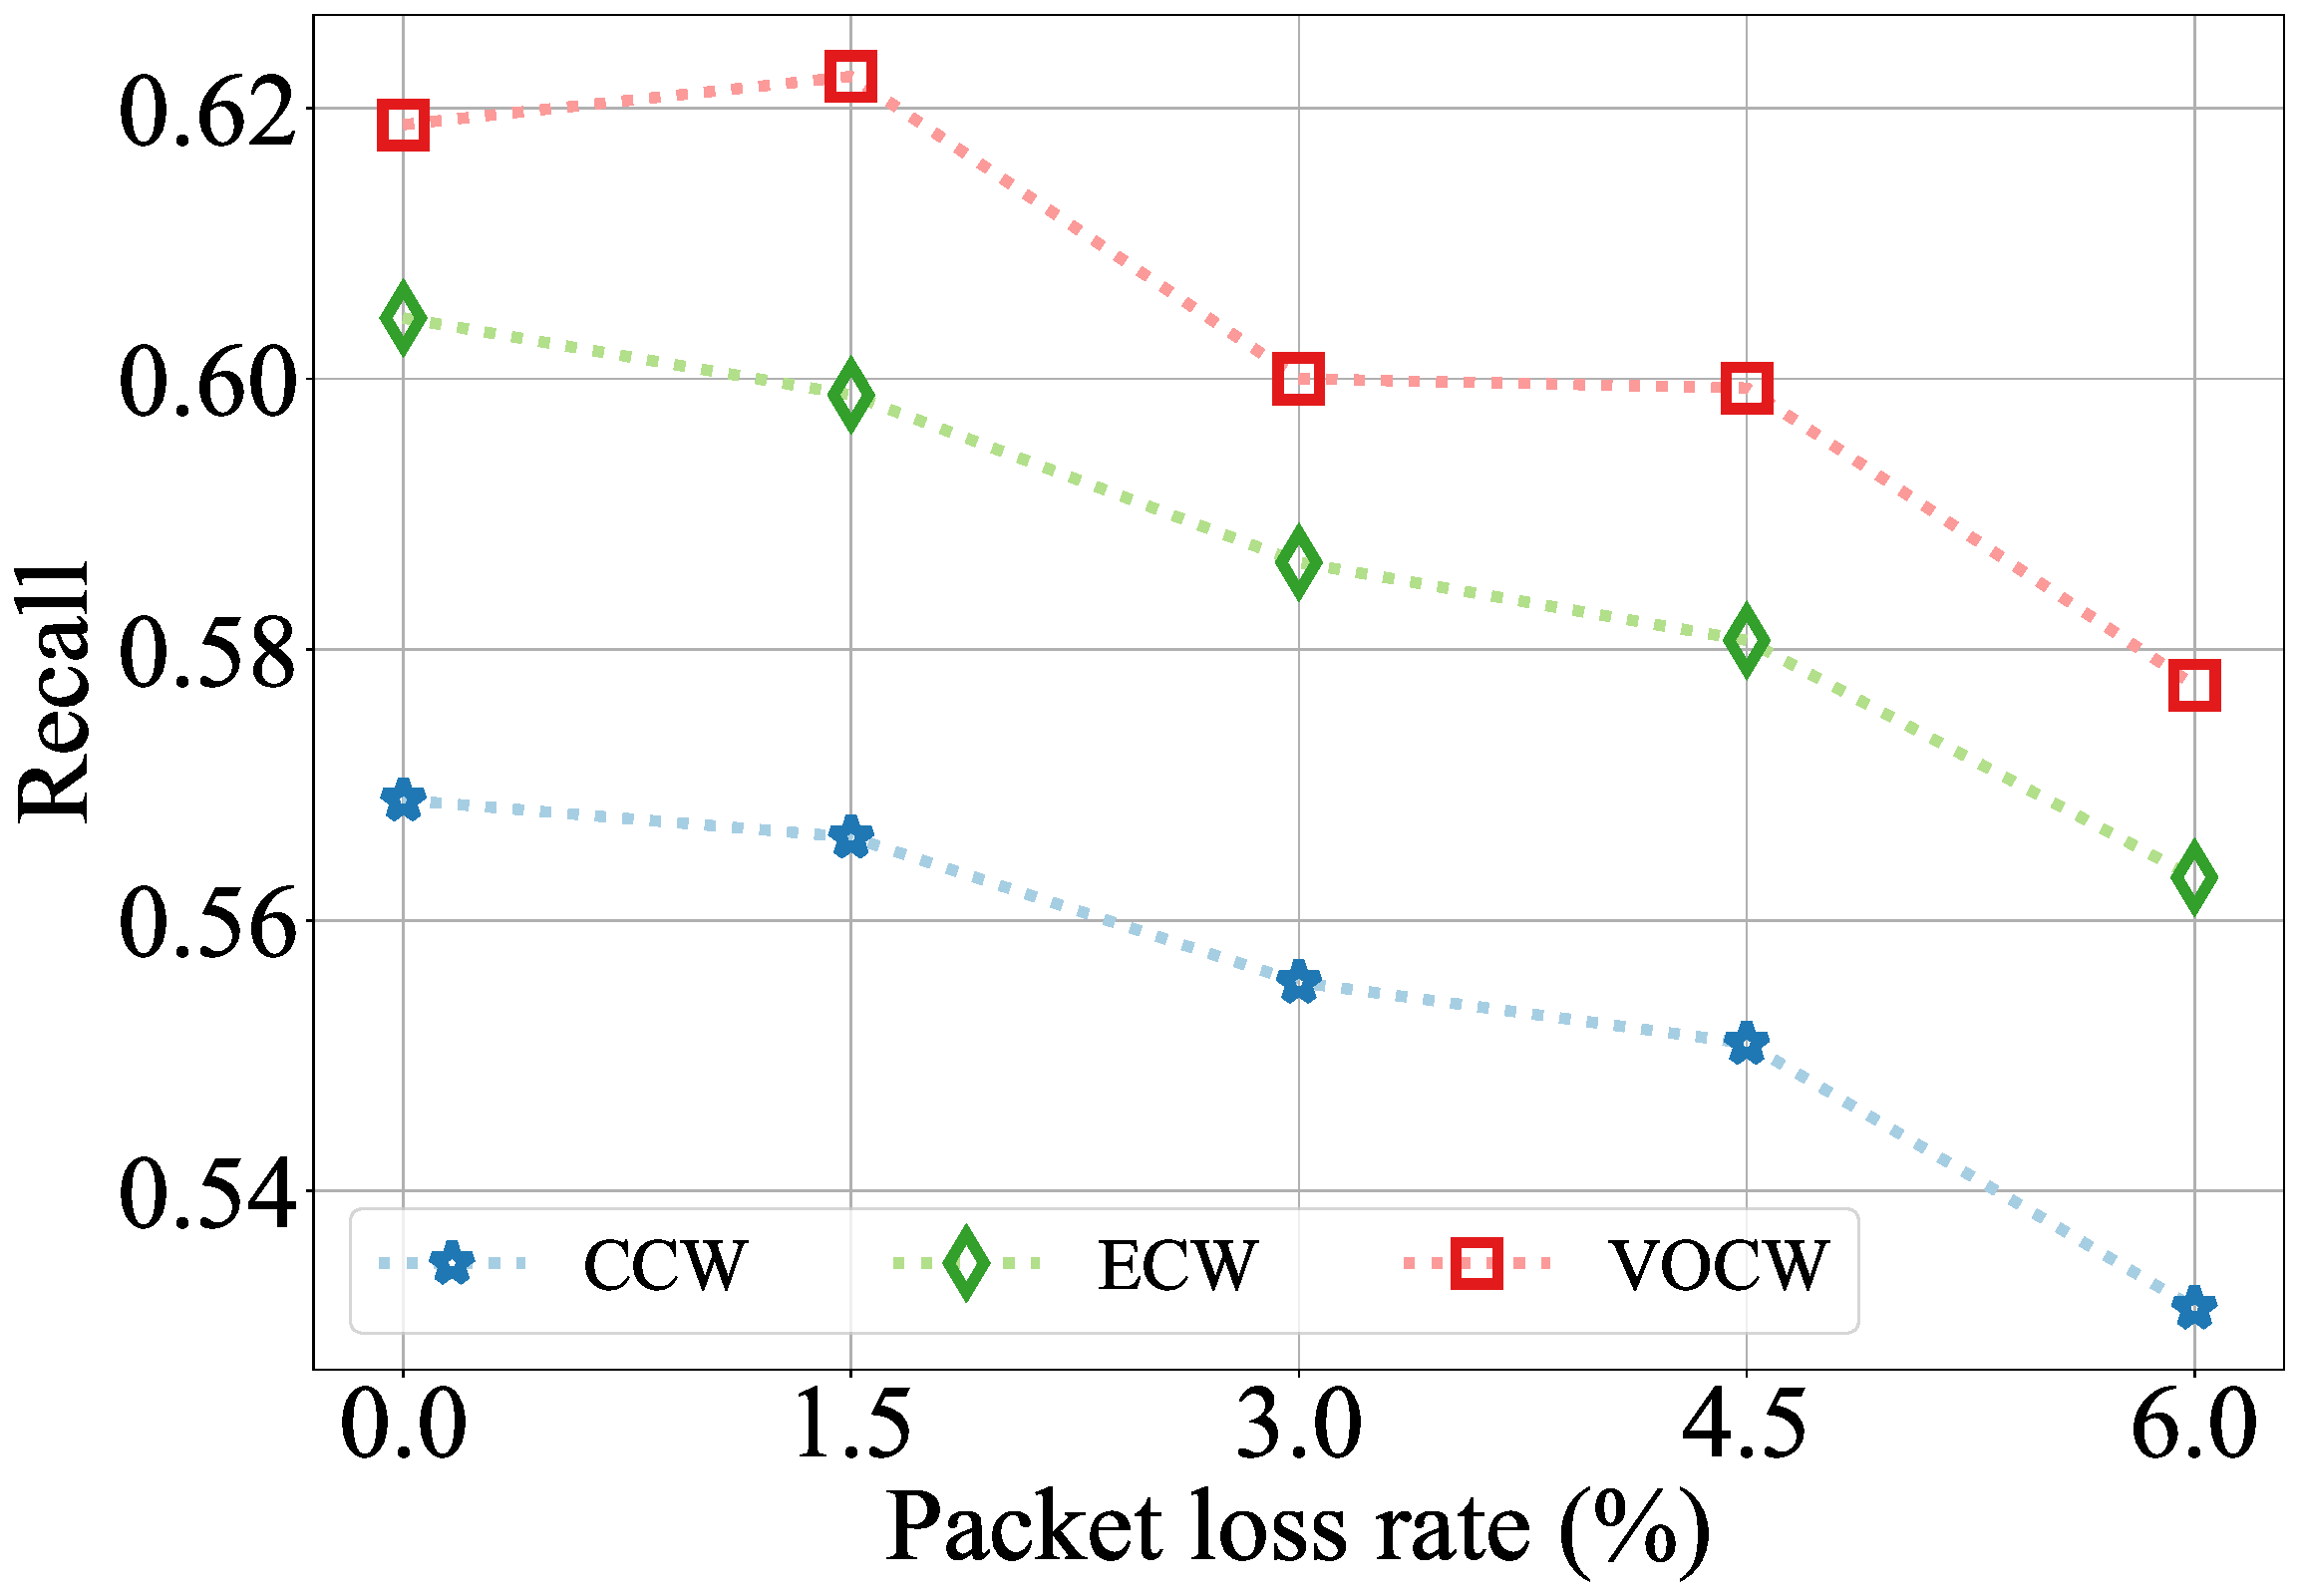
\includegraphics[width=0.33\columnwidth]{Fig5-7b-different-packet-loss-rate.pdf}}
     \subfloat[][]{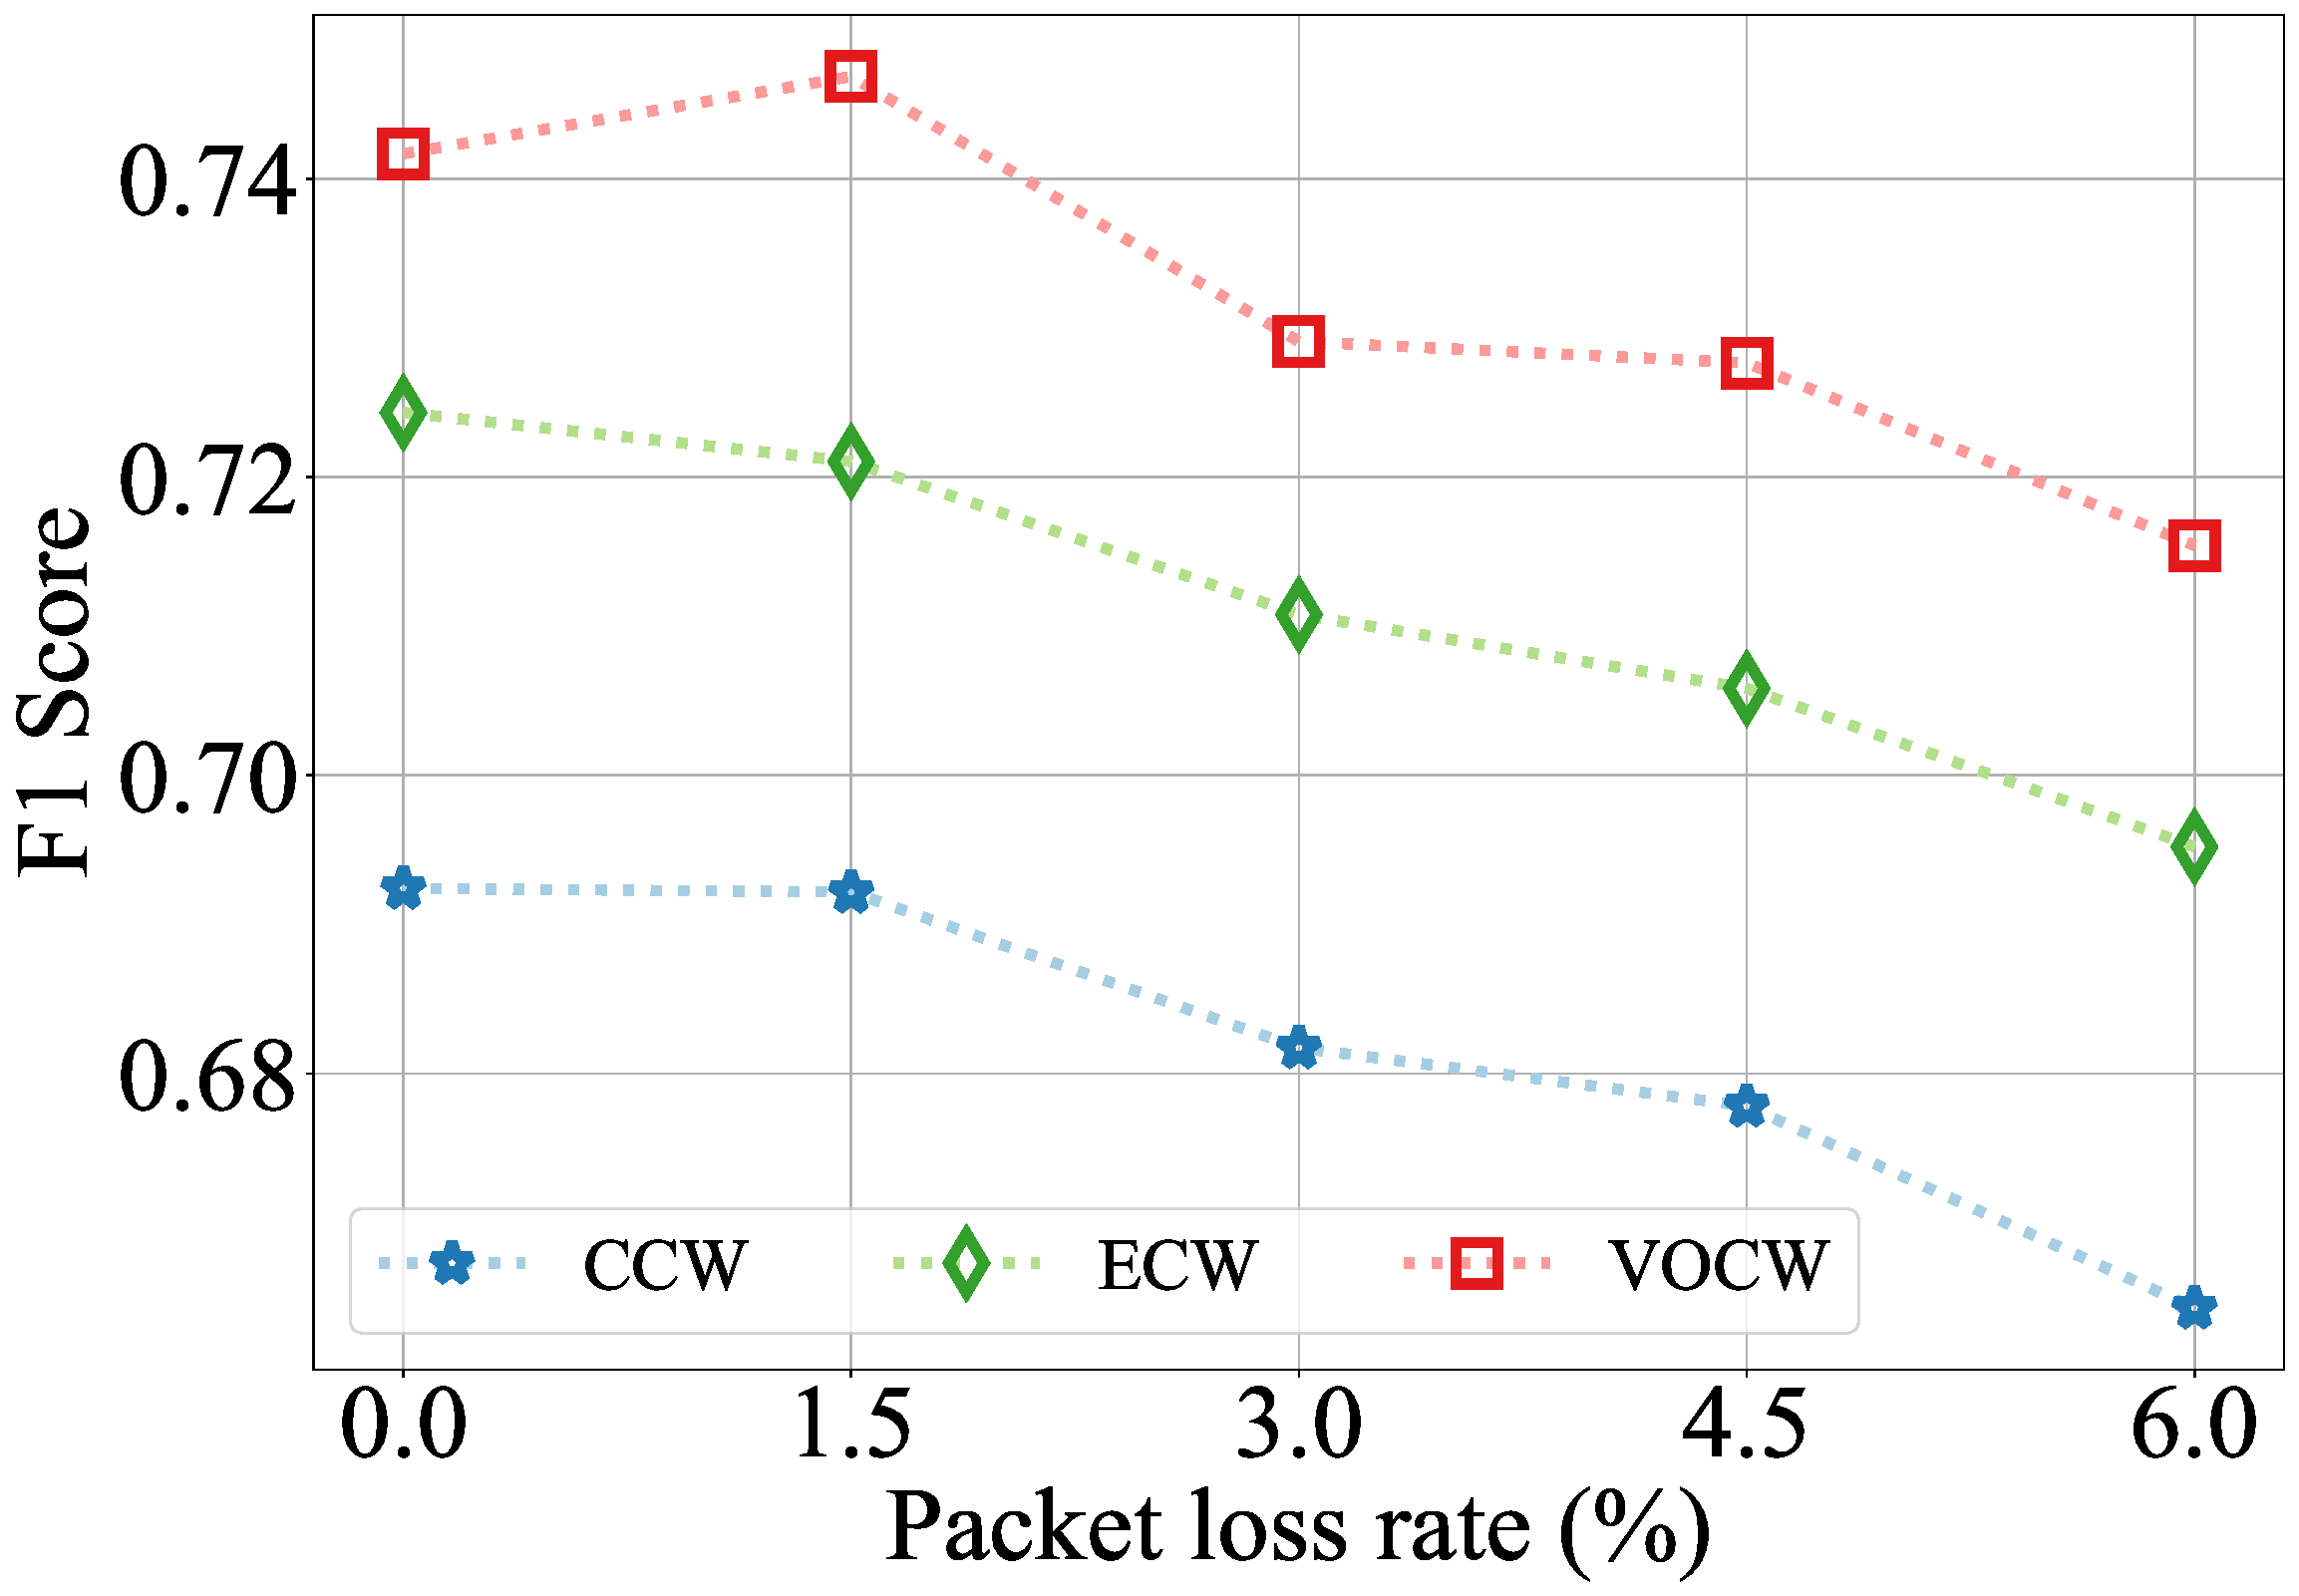
\includegraphics[width=0.33\columnwidth]{Fig5-7c-different-packet-loss-rate.pdf}}
     \bicaption[不同丢包率下的性能对比]{不同丢包率下的性能对比,其中丢包率从1\%增加至6\%。(a)查准率(b)查全率(c)F1值}[Performance comparison under different packet loss rate]{Performance comparison under different packet loss rate, which increases from 0\% to 6\%. (a) Precision (b) Recall (c) F1 score}
     \label{fig 5-6}
\end{figure}

\section{原型系统实现}\label{section 5-5}

本章节基于C-V2X 通信设备搭建硬件在环试验平台,并对C-V2X 端到端传输时延和丢包率等通信特征进行统计与分析。
进一步,搭建了基于无人小车的试验平台,并在其中部署了基于视图修正的碰撞预警算法。
最后,在真实复杂车联网通信环境下,基于无人小车和真实车辆,实现了超视距碰撞预警系统,并验证了所提原型系统的可行性与有效性。

\subsection{硬件在环试验平台}

\begin{figure}[h]
\centering
  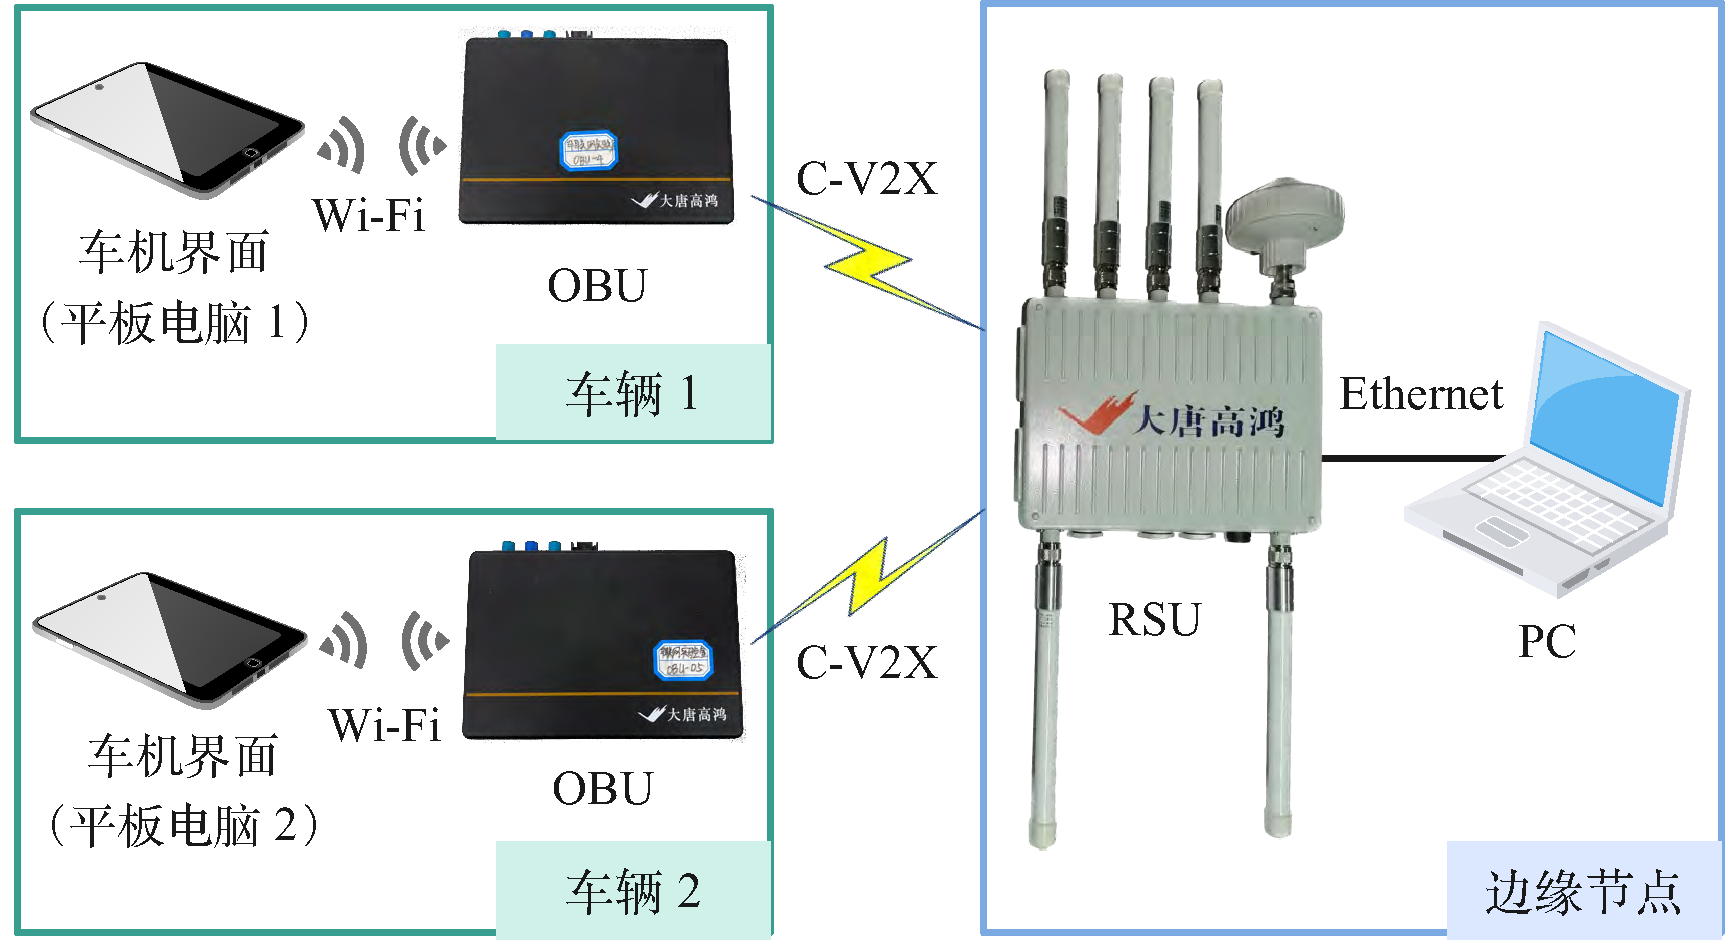
\includegraphics[width=1\columnwidth]{Fig5-8-hardware-in-the-loop-architecture.pdf}
  \bicaption[硬件在环平台框架]{硬件在环平台框架}[Hardware-in-the-loop platform framework]{Hardware-in-the-loop platform framework}
  \label{fig 5-7}
\end{figure}

\begin{figure}[h]
\centering
  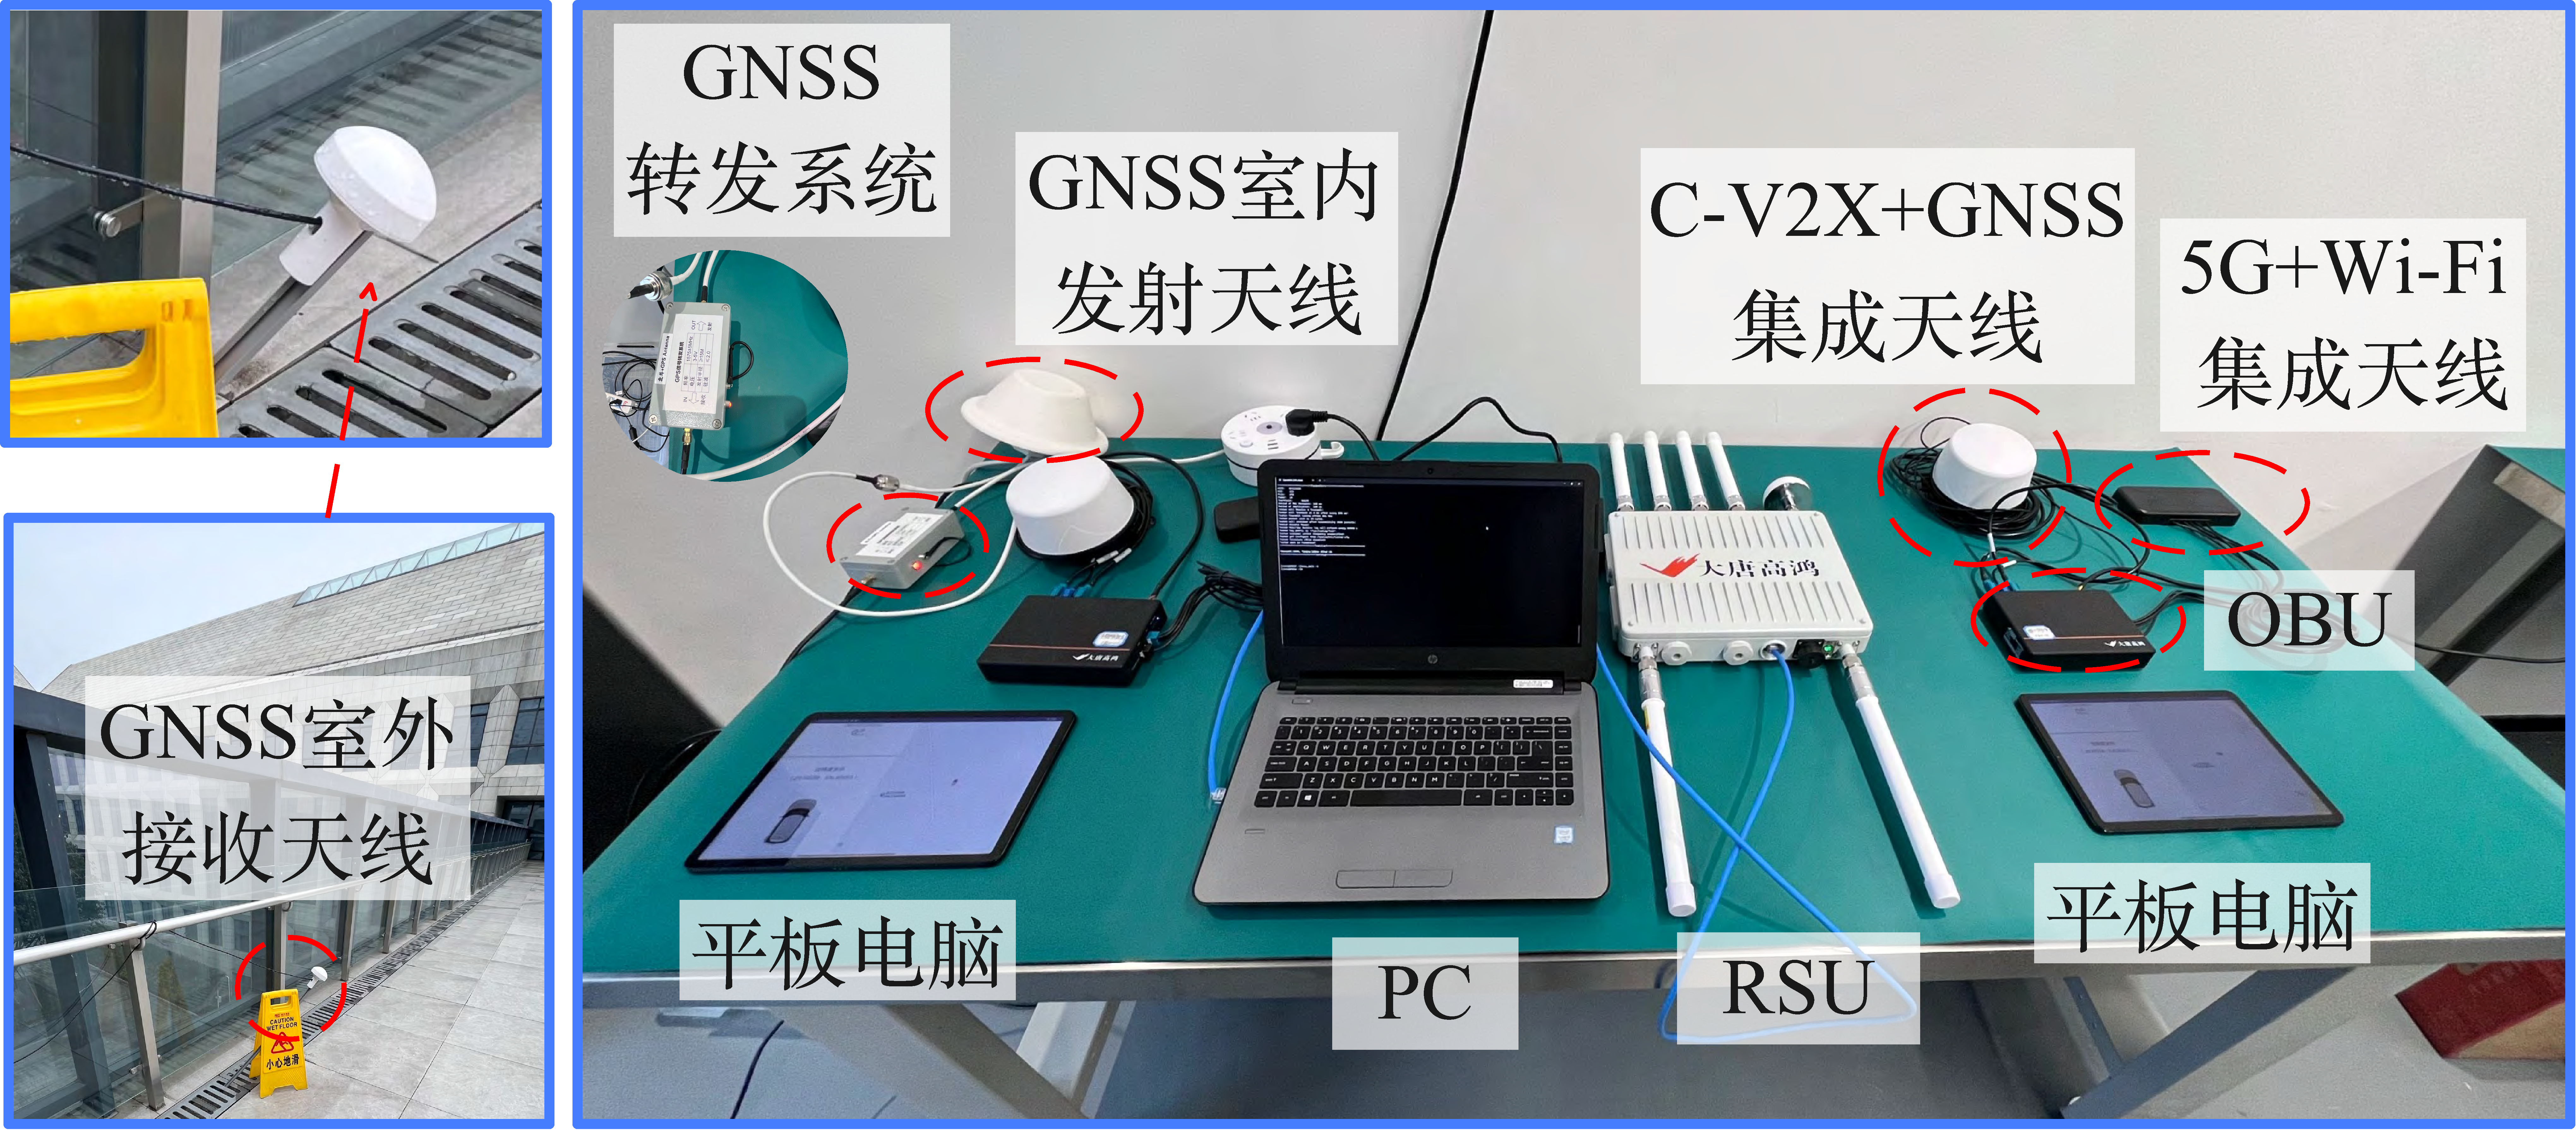
\includegraphics[width=1\columnwidth]{Fig5-9-C-V2X-hardware-in-loop.pdf}
  \bicaption[基于 C-V2X 的硬件在环试验平台]{基于 C-V2X 设备的硬件在环试验平台}[Hardware-in-the-loop platform based on C-V2X]{Hardware-in-the-loop platform based on C-V2X}
  \label{fig 5-8}
\end{figure}

基于 C-V2X 设备的硬件在环试验平台框架如图 \ref{fig 5-7} 所示。本系统中考虑了两辆车,每辆车配备一个 OBU,并有一个配备 RSU 的边缘节点。同时,一台具有一定计算能力的 PC 通过以太网与 RSU 相连,作为计算单元提供服务。车载平板电脑作为车机界面,通过 Wi-Fi 与 OBU 进行通信,并进行碰撞预警消息的可视化。基于 C-V2X 的硬件在环试验平台如图 \ref{fig 5-8} 所示。具体地,本平台采用的 OBU 和 RSU 均具备 LTE-V2X PC5 和 5G UU 双模通信能力,符合 3GPP R15 LTE-V2X 协议规范,并具有 GNSS 天线,可接收 GPS 卫星信号。在室内场景下,由于建筑物遮挡等原因,OBU 和 RSU 很难接收到 GNSS 信号,而 GNSS 数据报文中时间戳数据对于不同设备间的时间同步是至关重要的。因此,在室外廊桥上部署了 GNSS 接收天线,并通过有线方式连接 GNSS 信号转发系统。室内发射天线将 GNSS 信号进行转发,解决了室内 GNSS 信息弱甚至缺失的问题。

\begin{figure}[h]
\centering
  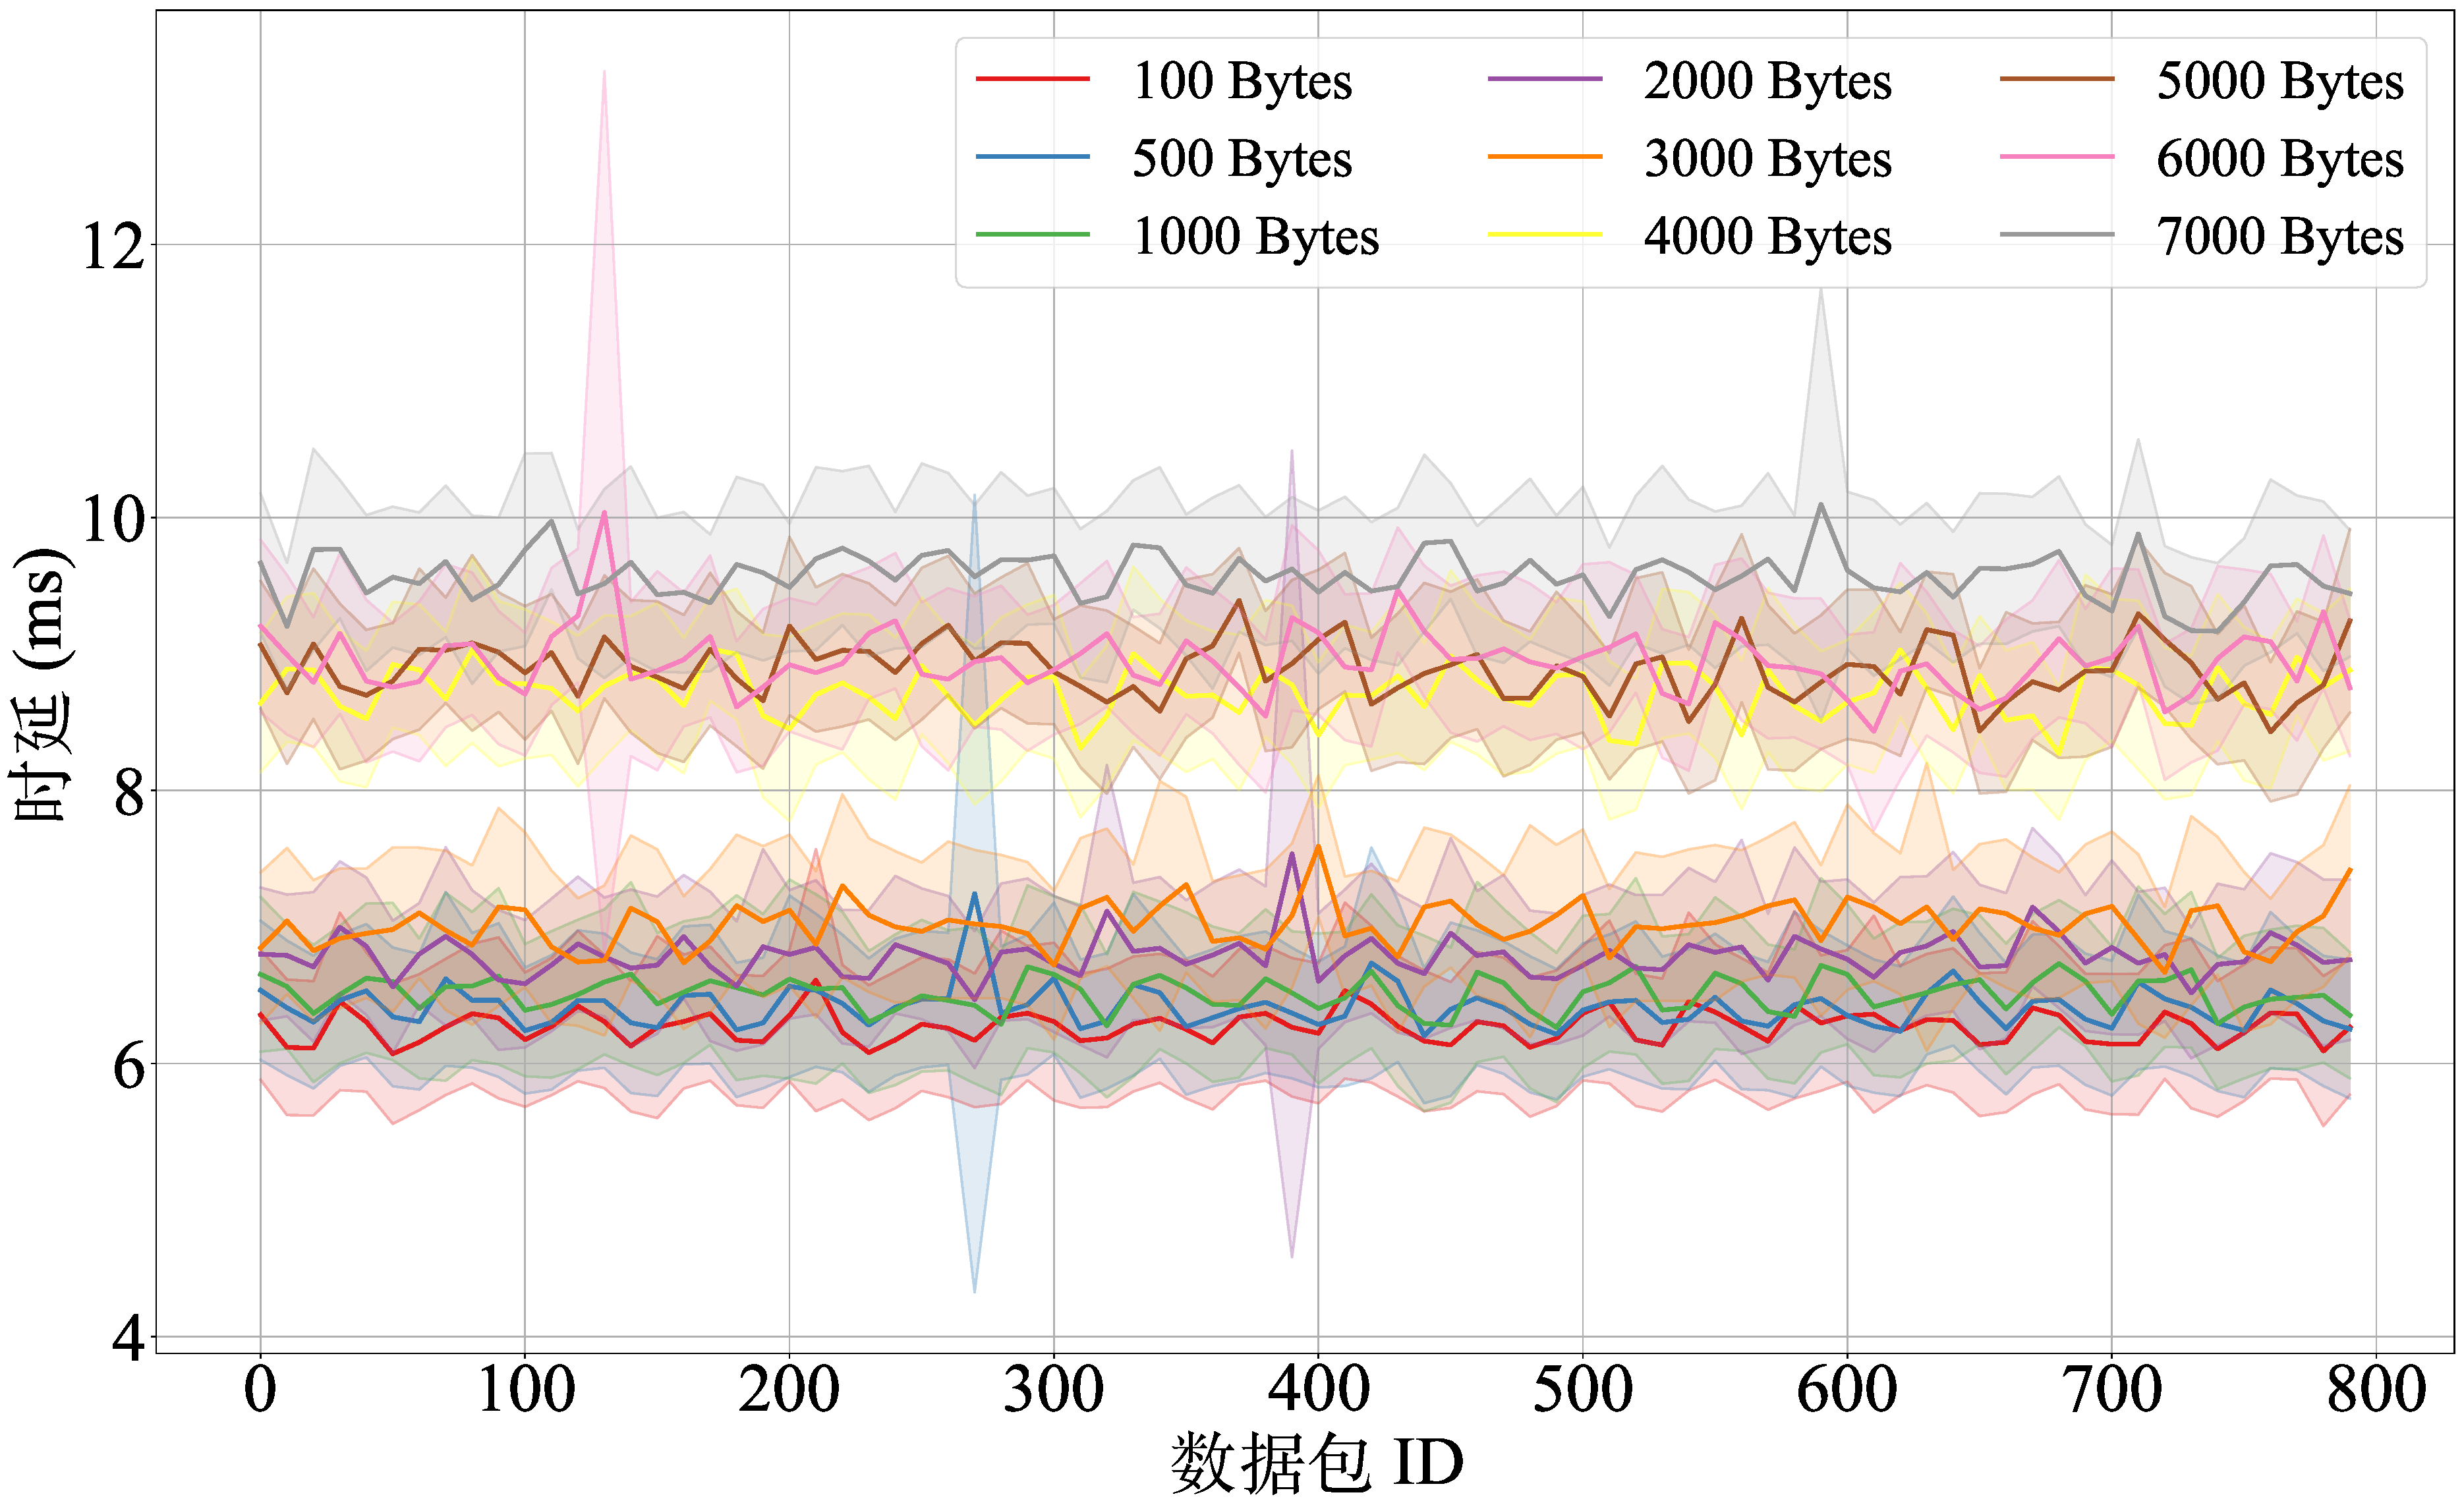
\includegraphics[width=0.9\columnwidth]{Fig5-10-delays.pdf}
  \bicaption[不同数据包大小下的C-V2X端到端时延比较]{不同数据包大小下的C-V2X端到端时延比较}[C-V2X end-to-end delay comparison under different packet data size]{C-V2X end-to-end delay comparison under different packet data sizes}
  \label{fig 5-9}
\end{figure}

基于硬件在环试验平台,采集了不同数据包大小下C-V2X从OBU到RSU的端到端传输时延数据。具体地,以10 Hz的频率分别发送1000个数据包,单个数据包大小从100 Bytes增加至7000 Bytes以采集传输时延。图\ref{fig 5-9}比较了不同数据包大小下的C-V2X端到端时延。虽然传输时延具有一定的波动性,但最小数据包(100 Bytes)和最大数据包(7000 Bytes)的平均传输时延仍然最小(6.271 ms)和最大(9.570 ms)。当数据包大小从3000 Bytes增加到4000 Bytes时,数据包传输时延出现了明显的跳跃式增长。在C-V2X通信环境中,超过3000 Bytes的数据包需要重新分包,导致传输时延显著增加。

\begin{table}[h]\small
\centering
\bicaption{不同数据包大小下C-V2X通信特征}{Different characteristics of C-V2X communications under different packet sizes}
\setlength{\tabcolsep}{4.5mm}{
\begin{tabular}{ccccccc}
\toprule
\begin{tabular}[c]{@{}c@{}}数据包大小\\(Bytes)\end{tabular}&\begin{tabular}[c]{@{}c@{}}平均时延\\(ms)\end{tabular}&\begin{tabular}[c]{@{}c@{}}最大时延\\(ms)\end{tabular}&\begin{tabular}[c]{@{}c@{}}最小时延\\(ms)\end{tabular}&\begin{tabular}[c]{@{}c@{}}时延\\方差\end{tabular}&\begin{tabular}[c]{@{}c@{}}丢包率\\(\%)\end{tabular}\\
\midrule
100& 6.271 & 8.975 & 5.396  & 0.292 & 0.0 \\
500& 6.411 & 15.889 & 5.133 & 0.375 & 0.0 \\
1000& 6.508 & 8.185 & 5.202 & 0.313 & 0.0 \\
2000& 6.796 & 16.286 & 5.561 & 0.415 & 0.1 \\
3000& 7.014 & 9.916 & 5.667 & 0.328 & 0.0 \\
4000& 8.708 & 10.607 & 7.620 & 0.322 & 6.7 \\
5000& 8.879 & 10.662 & 7.916 & 0.324 & 11.4 \\
6000& 8.944 & 19.654 & 7.547 & 0.455 & 8.5 \\
7000& 9.570 & 14.456 & 8.258 & 0.367 & 11.0 \\
\bottomrule
\end{tabular}}
\label{table 6-2}
\end{table}

针对采集的不同大小数据包的C-V2X端到端传输时延,本章进行了分析并统计了以下指标:平均时延、最大时延、最小时延、时延方差以及丢包率。其中,平均时延、最大时延和最小时延的单位为毫秒。时延方差表示了传输时延数据的离散程度。丢包率表示丢包数量占整体数据包数量的比例。不同数据包大小下的C-V2X通信特征显示在表\ref{table 6-2}中,可以看到随着数据包大小的增加,平均传输时延从6.271毫秒增加至9.570毫秒,同时,最小时延从5.396 ms增加至8.258ms。另一方面,可以得到不同数据包大小的时延方差均值为0.355,且其方差为0.0028。显然,不同数据包大小对于传输时延离散程度的影响是一致的。值得注意的是,当数据包大小增加至4000 Bytes及以上时,丢包率具有显著增长,从100$\sim$3000 Bytes大小数据包平均丢包率0.02\%增长至9.4\%(4000$\sim$7000 Bytes)。这是因为当数据包超过单个数据包的传输大小限制时,进行了数据重新分包传输,增加了传输次数,导致了传输过程中的丢包概率增加。

\subsection{超视距碰撞预警原型系统}

本章基于无人小车搭建了试验平台,如图\ref{fig 5-10}所示。无人小车配备NVIDIA Jetson AGX Xavier边缘计算单元,在Ubuntu 18.04操作系统上运行,并配备激光雷达、双目视觉传感器等传感器设备。同时,无人小车搭载了OBU,可以通过V2I通信将自身车辆状态信息上传至位于路侧的边缘节点。进一步,在基于安卓系统的平板电脑和基于Qt5平台的笔记本电脑上开发了车端应用和边缘设备软件,并实现并部署了基于视图修正的碰撞预警算法。基于无人小车试验平台,在真实复杂车联网环境中实现了超视距碰撞预警原型系统,如图\ref{fig 5-11}所示。

\begin{figure}[h]
\centering
  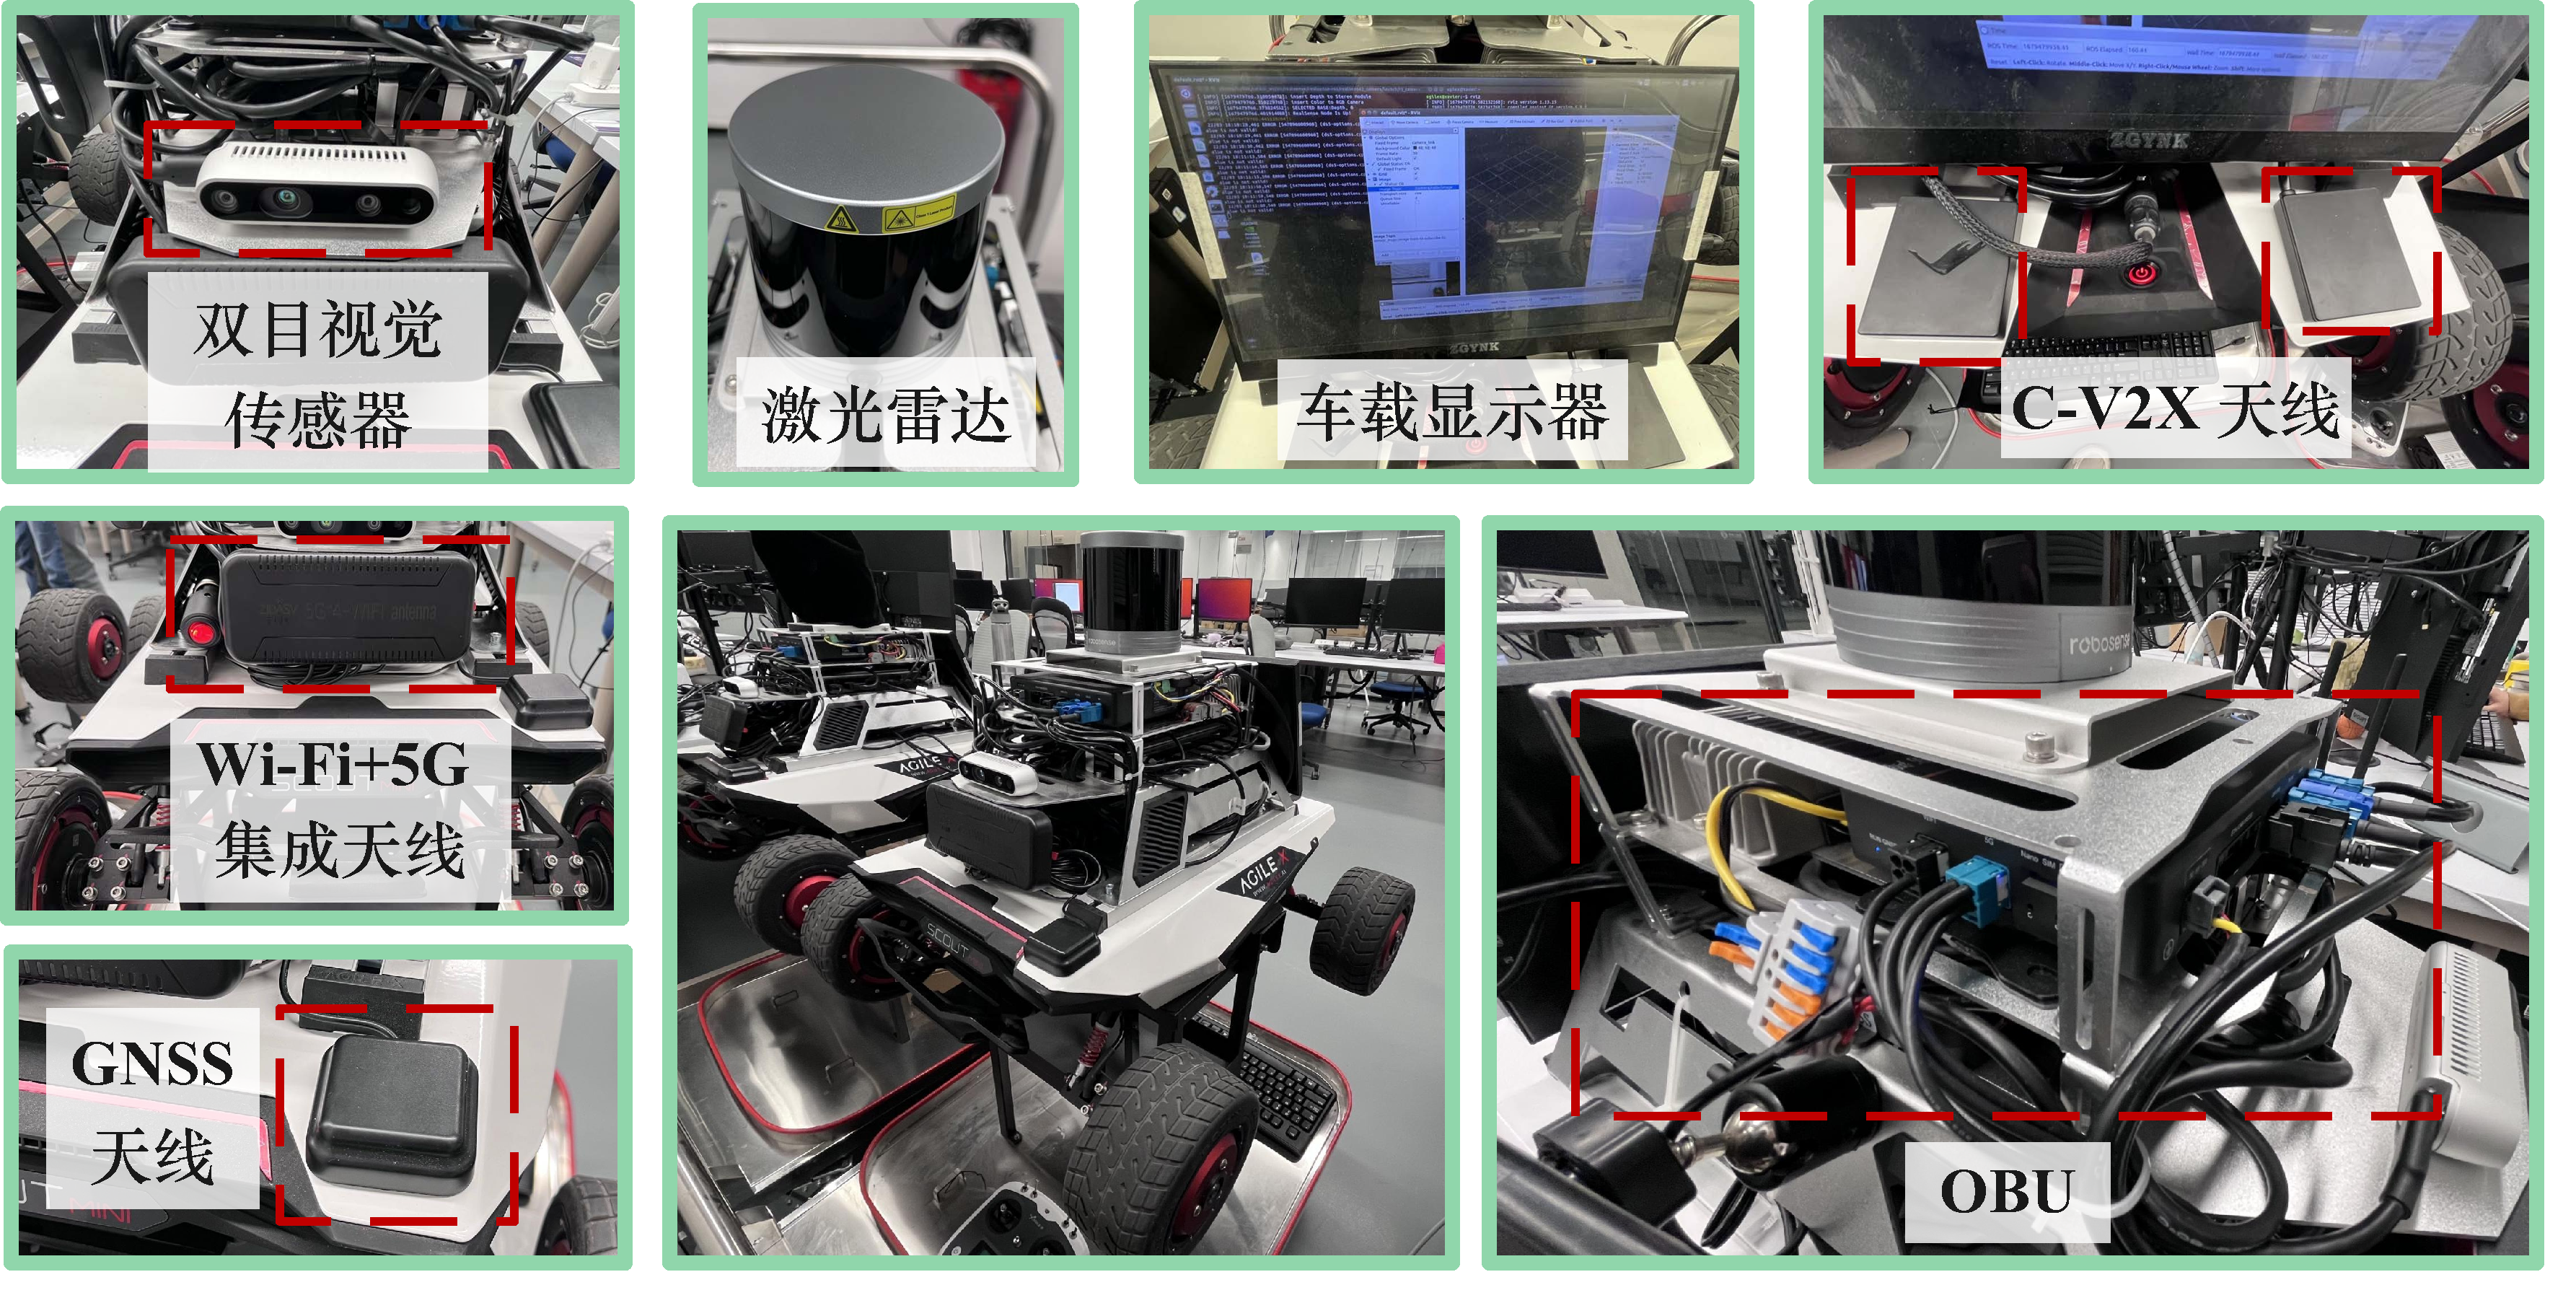
\includegraphics[width=1\columnwidth]{Fig5-11-unmanned-vehicle-platform.pdf}
  \bicaption[基于无人小车的试验平台]{基于无人小车的试验平台}[Experimental platform based on unmanned vehicles]{Experimental platform based on unmanned vehicles}
  \label{fig 5-10}
\end{figure}

\begin{figure}[h]
\centering
  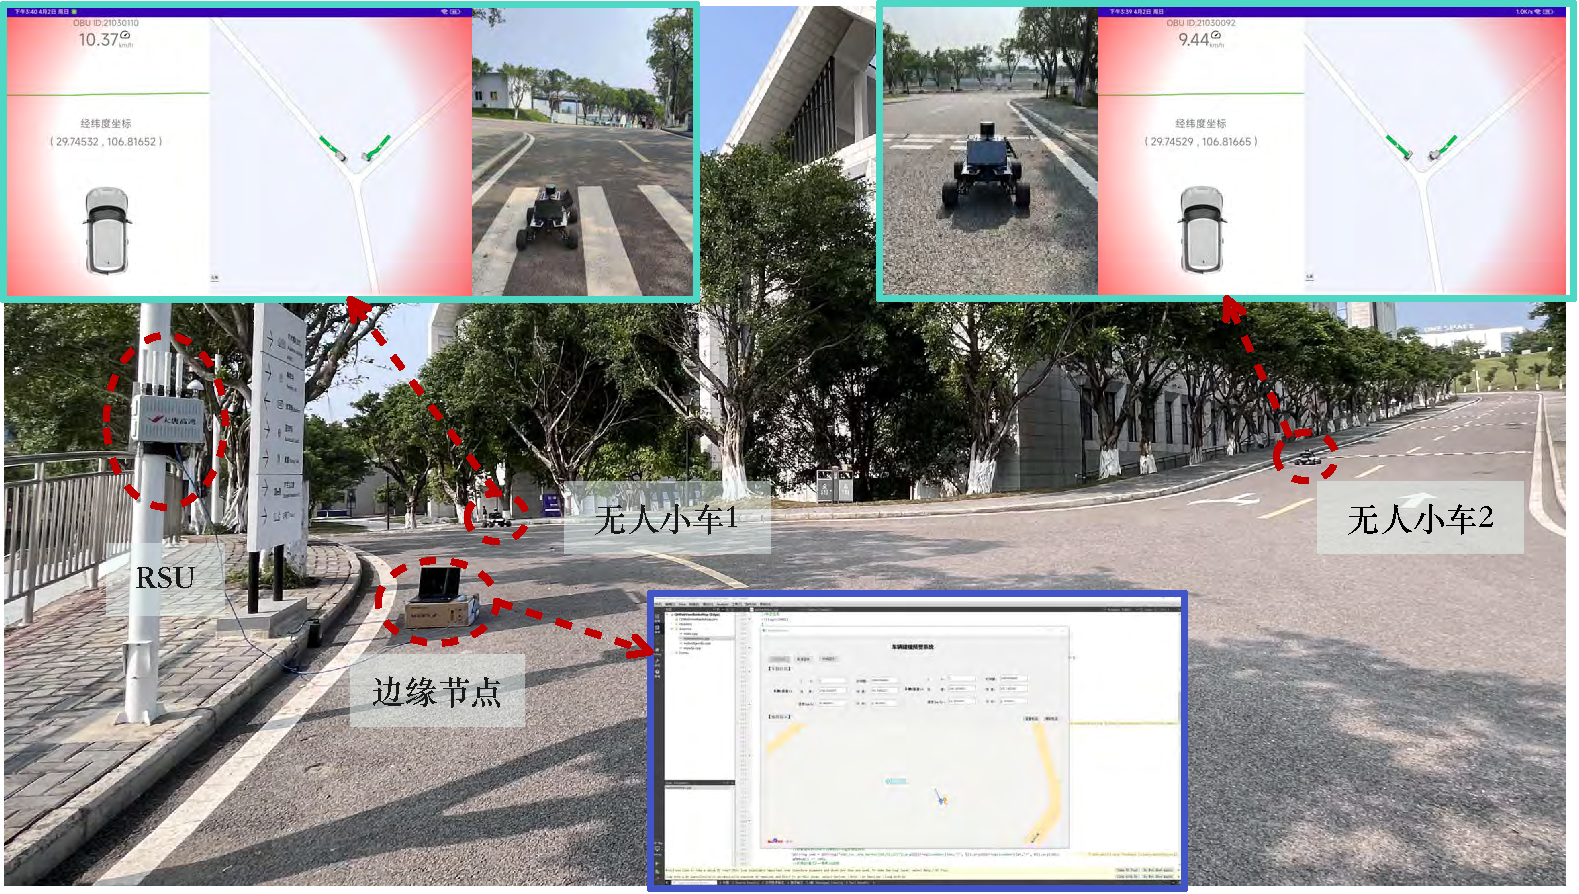
\includegraphics[width=1\columnwidth]{Fig5-12-outdoor.pdf}
  \bicaption[基于无人小车的超视距碰撞预警原型系统]{基于无人小车的超视距碰撞预警原型系统}[Non-light-of-sight collision warning prototype system based on unmanned vehicles]{Non-light-of-sight collision warning prototype system based on unmanned vehicles}
  \label{fig 5-11}
\end{figure}

\begin{figure}[h] 
	\centering
	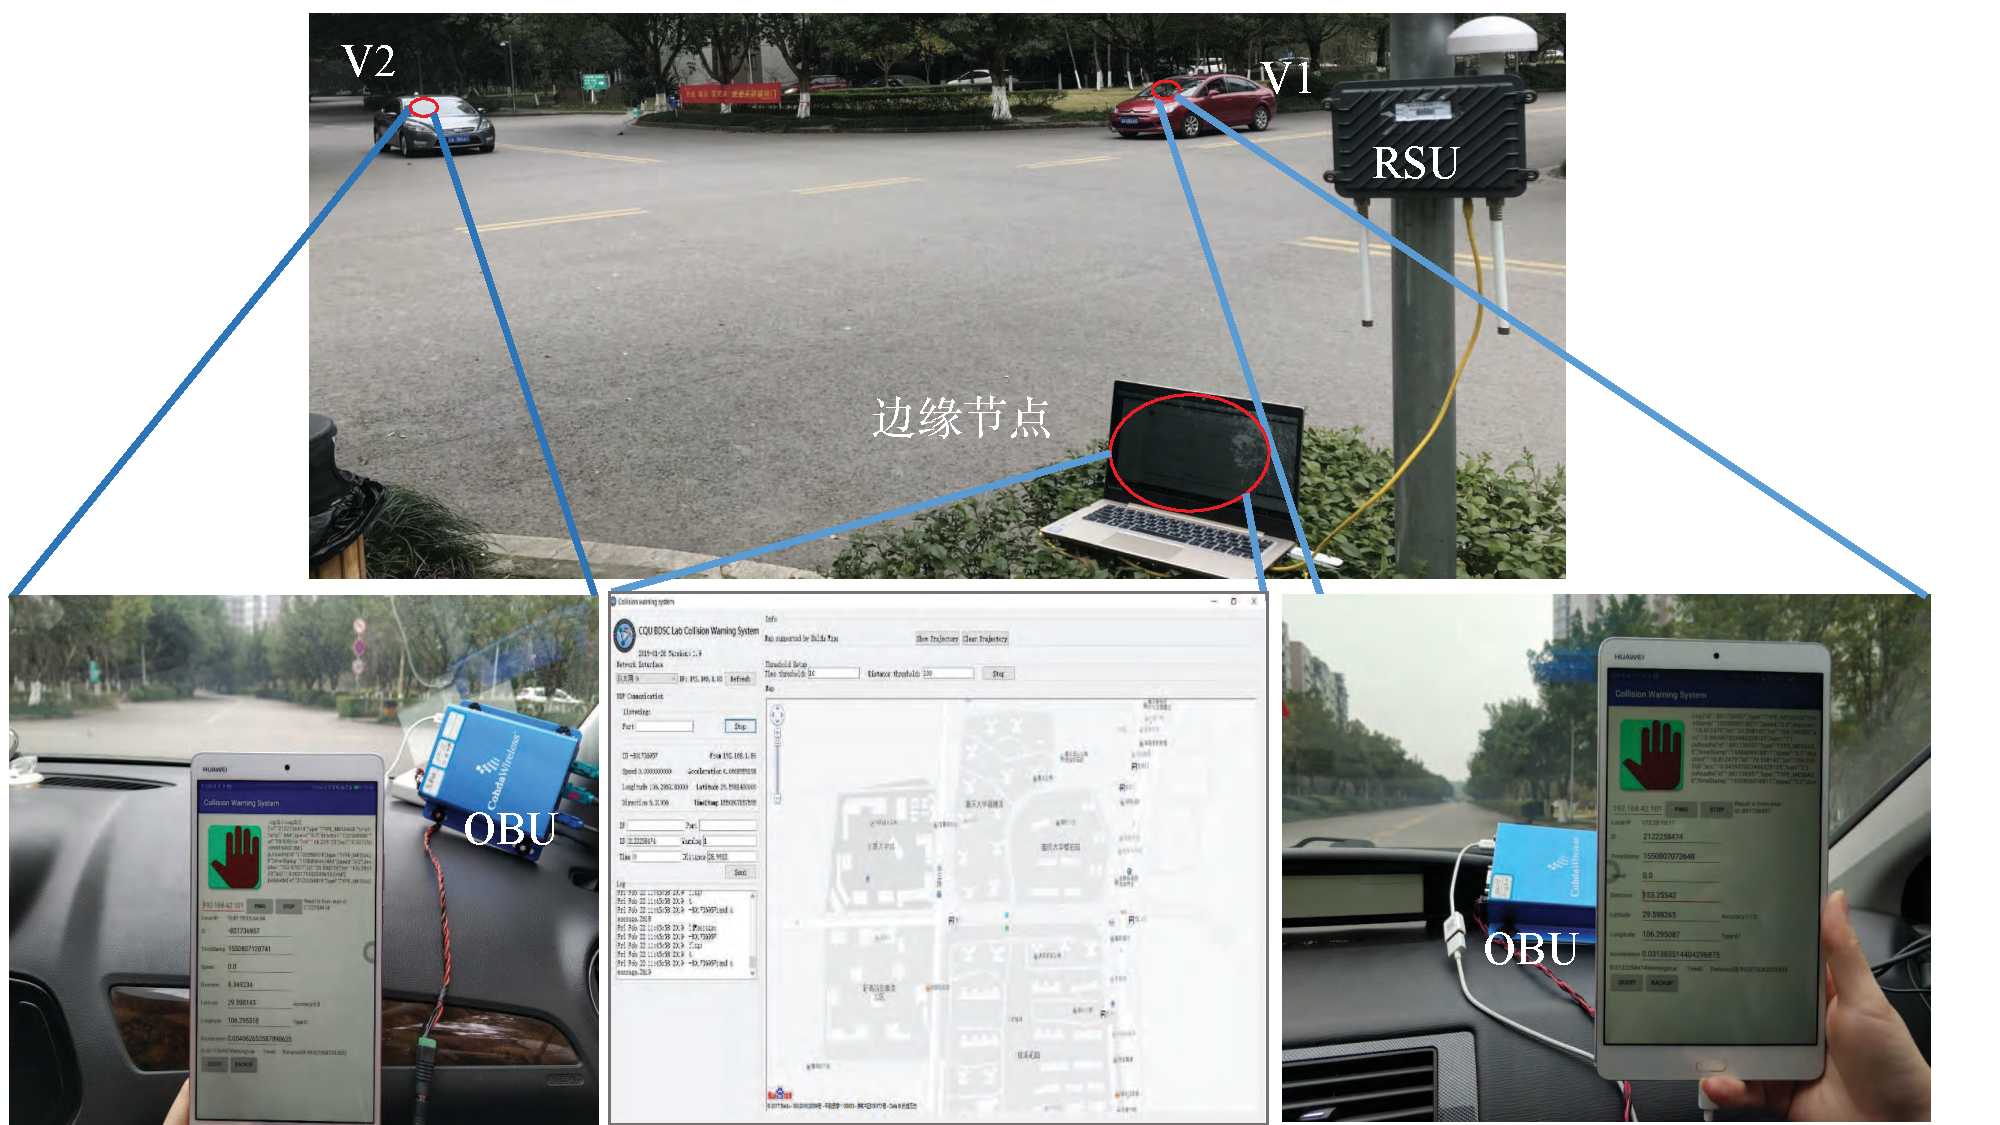
\includegraphics[width=1\columnwidth]{Fig5-12.pdf}
	\bicaption[基于真实车辆的超视距碰撞预警原型系统]{基于真实车辆的超视距碰撞预警原型系统}[Non-light-of-sight collision warning prototype system based on real vehicles]{Non-light-of-sight collision warning prototype system based on real vehicles}
	\label{fig 5-12}
\end{figure}

本系统旨在在两车之间有可能发生碰撞时触发警告信息,从而提高车辆的安全性。具体地,在三叉路口的基础设施上部署了RSU,通过网线将其与笔记本电脑相连并被视为边缘节点。边缘节点接收无人小车上传的状态信息,并使用基于视图修正的碰撞预警算法进行评估是否存在潜在碰撞风险。如果存在,则通过V2I通信将碰撞预警消息发送至无人小车并在车机界面中进行可视化。图\ref{fig 5-11}中左上和右上角分别展示了无人小车1和无人小车2的自身视角以及车机界面。可以看到,无人小车分别位于三叉路口中的两条支路上,由于地势的差异(无人小车1位于上坡路段,无人小车2位于下坡路段),两车无法通过基于视距的传感设备感知到彼此,因而具有潜在碰撞风险。当两辆车同时驶向路口时,边缘节点通过V2I通信接收车辆信息,并基于所提算法判断当前存在碰撞风险。随后,无人小车接收到预警信息,并在车机界面通过红色边框效果进行展示。

进一步,在真实车辆部署中实现了超视距碰撞原型系统,如图\ref{fig 5-12}所示,两辆汽车(即V1和V2)正在向十字路口移动,并相互靠近。每辆车都配备了一个OBU,其与一个基于安卓的平板电脑相连。本章开发了一个基于安卓系统的应用程序,用于收集车辆的实时状态,包括GPS坐标、速度、加速度、方向和时间戳等。车辆通过V2I通信向边缘节点更新其状态,根据从不同车辆收到的信息,边缘节点执行基于视图修正的碰撞预警算法。一旦检测到存在碰撞风险,预警信息就会被触发,并通过I2V通信传送给相应的车辆。随后,车辆中搭载的平板电脑上会显示一个停车标志,并伴随着振动和警告音。

\section{本章小结}\label{section 5-6}

本章提出了超视距碰撞预警场景,其中车辆周期性上传自身状态信息,边缘节点基于车辆信息构建逻辑视图以反映车辆实时状态,并在此基础上,为车辆提供碰撞预警服务。此外,本章提出了一种基于视图修正的碰撞预警算法,通过结合传输延迟估计和数据包丢失检测,校准逻辑视图以构建更加实时准确的逻辑视图。具体地,通过现场测试获得的V2I传输数据,推导一个基于稳定分布的传输时延拟合模型来估计传输时延,同时根据历史信息检测数据包丢失。建立了基于真实车辆轨迹的仿真模型,仿真结果表明所提VCCW算法相比于基于云和基于边缘的碰撞预警算法,在碰撞预警的查准率、查全率,以及F1值方面具有优势。最后,本章搭建了基于C-V2X的硬件在环试验平台,对C-V2X端到端传输性能进行了分析,并在真实复杂车联网环境中实现了超视距碰撞预警原型系统,验证了所提系统的可行性与有效性。

\chapter{总结与展望}\label{section 7}

车联网是通过网络技术将车辆、道路基础设施以及其他联网设备连接起来,实现车辆信息的互联互通及共享的新兴技术。
车联网有助于提高行车安全、促进交通顺畅、降低能源消耗、提升驾驶体验和推动智慧城市等方面,对于我国现代化城市建设和汽车产业发展都具有重要的推动作用。
同时,车载信息物理融合系统已成为支撑车联网中各类智能交通系统应用的关键。
本文致力于从服务架构融合、评估指标设计、资源协同优化、质量-开销均衡和原型系统实现五个方面协同驱动面向异构车联网的车载信息物理融合系统。
首先,面向高动态异构车联网,融合不同的计算范式与服务架构是实现车载信息物理融合的基础。
其次,面向分布式时变物理环境,有效的数据获取与建模评估是驱动车载信息物理融合的核心。
再次,面对动态异构节点资源,高效的任务调度与资源分配是进一步提升ITS服务质量的关键。
另外,面向多元智能交通系统应用需求,满足差异性的系统质量与系统开销需求是驱动车载信息物理融合的另一关键。
最后,面向复杂的真实车联网环境,基于车载信息物理融合系统进行有效设计并实现具体系统原型是具有挑战的。
本文的主要贡献如下:

\circled{1} 基于软件定义网络和边缘计算的异构车联网架构研究。
首先,将SND与边缘计算融入车联网服务架构,旨在最大化SDN逻辑上集中控制与分布式边缘计算服务的协同效应。
具体地,设计了包括应用层、控制层、虚拟层以及数据层的车联网分层服务架构,通过SDN思想将控制平面与数据平面分离实现逻辑上的集中控制,利用分布式边缘计算服务的异构资源进一步增强系统性能。
其次,针对所提服务架构分析了其中的挑战与机遇,并进一步提出跨层协议栈对未来研究方向进行讨论。
最后,通过两个典型应用的案例研究,验证了所提服务架构的巨大潜力以及对下一代智能交通系统发展提供启示。

\circled{2} 面向车载边缘计算的VCPS评估指标(Age of View)设计与优化策略研究。
首先,提出了面向车载边缘计算的协同感知与异质信息融合框架,其中边缘节点通过融合车辆感知信息构建边缘视图以反映实时车联网环境。
其次,建立了基于多类M/G/1优先队列的感知信息排队模型,并进一步基于异质信息的时效性、完整性和一致性建模设计了崭新的车载信息物理融合评估指标(Age of View),并形式化定义了视图质量最大化问题。
再次,提出了基于差分奖励的多智能体强化学习(MADR)算法,其中车辆动作空间包括信息感知频率与上传优先级,边缘节点基于车辆预测轨迹和视图需求分配V2I带宽,并通过基于差分奖励的信用分配机制评估车辆对于视图构建的贡献。
最后,仿真实验结果表明,MADR算法能有效提高车载信息物理融合系统的质量。

\circled{3} 面向NOMA车载边缘计算的异构资源协同优化策略研究。
首先,提出了基于NOMA的车载边缘计算框架,其中边缘节点协同分配异构资源以对计算任务进行实时处理。
其次,考虑了NOMA车联网中域内和域间干扰,建立了V2I传输模型,并形式化定义了最大化任务服务率的协同资源优化问题。
再次,将协同资源优化问题分解为任务卸载与资源分配子问题,其中将任务卸载子问题建模为严格势博弈模型,并进一步提出多智能体分布式深度确定性梯度策略(MAD4PG)算法来实现纳什均衡,另一方面,将资源分配子问题分解为两个独立凸优化问题,并分别使用基于梯度的迭代方法和KKT条件得到最优解。
最后,仿真实验结果表明,MAD4PG算法能最大化异构资源利用率,能有效提高任务完成率。

\circled{4} 面向车载信息物理融合的质量/开销均衡优化策略研究。
首先,提出了车载信息物理融合框架,其中边缘节点基于车辆感知信息对车联网中物理实体建立相应的数字孪生模型。
其次,考虑数字孪生的及时性、一致性和冗余度,以及感知与传输开销,建立了车载信息物理融合系统质量和开销模型,并进一步形式化定义了最大化VCPS质量且最小化VCPS开销的双目标优化问题。
再次,提出了多智能体多目标强化学习(MAMO)算法,其中提出了决斗评论家网络,基于状态价值和动作优势来评估智能体的动作。
最后,仿真实验结果表明,MAMO算法可以实现VCPS质量和开销均衡以满足不同的智能交通系统应用需求。

\circled{5} 基于车载信息物理融合的超视距碰撞预警原型系统设计与实现。
首先,提出了超视距碰撞预警场景,其中车辆由于非视距(NLOS)问题存在潜在碰撞风险,亟需提出基于V2X通信的碰撞预警解决方案。
其次,提出基于视图修正的碰撞预警(VCCW)算法,具体地,基于现场测试获得的V2I应用层传输时延数据,建立了基于稳定分布的V2I时延拟合模型。
另一方面,设计了基于数据上传频率和车辆状态历史信息的无线传输丢包检测机制。
通过时延估计和丢包检测对视图进行修正,以提供更加准确实时的碰撞预警服务。
再次,仿真实验结果表明,VCCW能有效提高碰撞预警的查准率和查全率。
最后,搭建了基于C-V2X的硬件在环试验平台,对C-V2X端到端时延进行了分析,进一步基于无人小车搭建了验证平台,部署了VCCW算法并在真实复杂车联网环境中实现了超视距碰撞预警原型系统,验证了VCCW算法的有效性。

本文主要针对面向异构车联网的车载信息物理融合系统关键技术开展了研究,并取得了一定的成果。
但作为探索VCPS的早期阶段,本文工作无法完全解决所有挑战,有待进一步探索和解决。
在未来工作中,本文将进一步研究边缘节点之间的合作,以扩大支持的ITS应用,并提高整体系统的性能。
其次,通过考虑车辆移动性和边缘节点之间合作计算的内在关系来进一步提高系统性能。
此外,将考虑车联网端边云架构,通过利用车辆、边缘节点和云协同来提高性能。

%\include{contents/yourFreeChoise}


\backmatter %%% 后置部分(致谢、参考文献、附录等)

%% 参考文献
% 顺序编码制:cqunumerical		
% 注意:至少需要引用一篇参考文献,否则下面两行会引起编译错误。
\bibliographystyle{cqunumerical}
\bibliography{ref/refs}


%% 附录(按ABC...分节,证明、推导、程序、个人简历等)
\appendix

% 个人简历
\chapter{附\hskip\ccwd{}录}
\section{作者在攻读博士学位期间发表和拟发表论文目录}

下面是盲审标记\cs{secretize}的用法,记得去\textsf{main.tex}开启盲审开关看效果:

\begin{enumerate}
	\item 这是科研项目的名字 科研人员1,科研人员2,指导老师1,指导老师2,2017年5月30日
	\item 这一条与上一条内容相同,但进行了盲审标记 \secretize{科研人员1},\secretize{科研人员2},\secretize{指导老师1},\secretize{指导老师2},2017年5月30日
\end{enumerate}

\section{作者在攻读博士学位期间参加的科研项目}

下面是工具函数\cs{xuhao}的用例:

\xuhaotype[1]
\xuhao[1] \xuhao \xuhao \xuhao \xuhao \xuhao[1] \xuhao \xuhao \xuhao \xuhao

\setxuhao[2]
\xuhao[1] \xuhao \xuhao \xuhao \xuhao \xuhao[1] \xuhao \xuhao \xuhao \xuhao

\setxuhao[3]
\xuhao[1] \xuhao \xuhao \xuhao \xuhao \xuhao[1] \xuhao \xuhao \xuhao \xuhao

\setxuhao[4]
\xuhao[1] \xuhao \xuhao \xuhao \xuhao \xuhao[1] \xuhao \xuhao \xuhao \xuhao

\setxuhao[5]
\xuhao[1] \xuhao \xuhao \xuhao \xuhao \xuhao[1] \xuhao \xuhao \xuhao \xuhao

\setxuhao[6]
\xuhao[1] \xuhao \xuhao \xuhao \xuhao \xuhao[1] \xuhao \xuhao \xuhao \xuhao

\subsection{测试第三级目录2}
\subsubsection{四级目录1}
水陆草木之花,可爱者甚蕃。晋陶渊明独爱菊。自李唐来,世人盛爱牡丹。予独爱莲之出淤泥而不染,濯清涟而不妖,中通外直,不蔓不枝,香远益清,亭亭净植,可远观而不可亵玩焉。
\subsubsection{四级目录2}
予谓菊,花之隐逸者也;牡丹,花之富贵者也;莲,花之君子者也。噫!菊之爱,陶后鲜有闻。莲之爱,同予者何人?牡丹之爱,宜乎众矣!
\subsubsection{四级目录3}
予谓菊,花之隐逸者也;牡丹,花之富贵者也;莲,花之君子者也。噫!菊之爱,陶后鲜有闻。莲之爱,同予者何人?牡丹之爱,宜乎众矣!

\section{关于声明书和授权书}
声明和授权部分支持扫描页替换,请在\pkg{main.tex}中设置。

\section{程序源代码}
以下是一段供排版测试的Python程序源代码:
\begin{Python}
# 这是一行注释

import pandas as pd
import matplotlib.pyplot as plt
import numpy as np
import seaborn as sns
import os

lengthSummary = pd.DataFrame()
lengthSum = lengthPool.groupby(['Pretreatment','Atmosphere'])
for name, group in lengthSum:
	sumBuffer = group.describe()
	sumBuffer.columns = [(name[0]+' '+name[1])]
	lengthSummary = pd.concat([lengthSummary,sumBuffer], axis = 1)
lengthSummary.to_csv('lengthSummary.csv')

\end{Python}

以下是一段供排版测试的C++源代码:

\begin{C++}
#include <vector>
#include <algorithm>
#include <iterator>
std::vector<int> target2(5);
std::vector<int> target3;
template <typename RangeOfInts>
void foo(RangeOfInts source)
{
	std::vector<int> target1{std::begin(source),
		std::end(source)};
	std::copy(std::begin(source), std::end(source),
	std::begin(target2));
	std::copy(std::begin(source), std::end(source),
	std::back_inserter(target3));
}
\end{C++}

\section{附录的图和表}
以下内容用来测试附录中的插图和插表是否正常,主要的关注点在题注:

\begin{figure}[tbh]
\centering

\includegraphics[width=0.5\linewidth]{CQUbadge}
\caption{附录插图测试}
\label{fig:cqubadge}
\end{figure}

\begin{figure}[tbh]
	\centering
	
\includegraphics[width=0.5\linewidth]{CQUbadge}
	\caption{附录插图测试}
	\label{fig:cqubadge2}
\end{figure}

\begin{table}[htb]
	\centering\colsep[24pt]
	\caption{本课题研究的两个自变量}
	\label{tab:inroVarible}
	\begin{tabularx}{\linewidth}{cl}
		\toprule
		\headcell{自变量} & \headcell{自变量可取的值} \\
		\midrule\setxuhao[6]
		是否接触大气 & \xuhao[1] 接触大气 \xuhao 氮气保护 \\\setxuhao[2]
		溶解方式 & \xuhao[1] 超声30min \xuhao 搅拌1h \xuhao 静置12h\\
		表格的第三行 & \bigcell{使用\cs{bigcell}\\可主动换行}\\
		\bottomrule
	\end{tabularx}
\end{table}

\begin{equation}
\alpha\beta\gamma\delta\epsilon\varepsilon\zeta\eta = AB\Gamma\varGamma Z
\end{equation}\eqlist{附录中的公式编号1,双语}[Equation name in English A]

\begin{equation}
\alpha\beta\gamma\delta\epsilon\varepsilon\zeta\eta = CD\Gamma\varGamma Z
\end{equation}\eqlist{附录中的公式编号2,双语}[Equation name in English B]

测试用途:theequation值为:\theequation ,thefigure值为:\thefigure ,thetable值为:\thetable


%% 原创声明和授权说明书,可选:用扫描页替换
%\cquauthpage[contents/authscan.pdf]
%\cquauthpage

%% 致谢
\chapter[致\hskip\ccwd{}\hskip\ccwd{}谢]{{\CJKfontspec{SimHei}\zihao{3}致\hskip\ccwd{}\hskip\ccwd{}谢}}

% 这里用盲审环境包裹致谢,在开启盲审开关时,环境内部的内容不予渲染。
\begin{secretizeEnv}

提笔之际,已到了在重庆生活学习的第六个年头,而我的博士研究生学习阶段也可以说算是告一段落。回想读博期间一路走来,其中有欣喜,也有难过;有深深的孤独,也有现在的恋恋不舍。如今终于到了要道别的时候,所以想借此机会给每一个支持和帮助我的人们好好说一声感谢与有缘再见。

首先,我要衷心感谢我的导师刘凯教授。您是我学术道路上的引路人,您的悉心指导对我产生了巨大影响。您的专业知识、学术见解和研究激情都激发了我不断超越自我的动力。您耐心地解答我的问题,指导我的实验,并对我的论文提出宝贵的建议。您对我的信任和鼓励使我更加自信地迈向学术领域的新阶段。我将永远铭记您对我的慷慨付出和关心。

其次,我要感谢西南交通大学戴朋林老师、重庆邮电大学张浩老师、重庆师范大学肖颗老师、重庆大学国家卓越工程师学院李楚照老师,以及实验室廖成武、金飞宇、任华玲、刘春晖、晏国志、胡峻菠、钟成亮、吴峻源等同学在本学位论文撰写和校对过程中提供的宝贵意见与无私帮助。

再次,我要感谢我的母亲刘菁女士。您生育抚养了我,感谢您对我的无私包容与关爱支持,如果可以,我希望把这篇论文献给您。您是我所见过最坚强的人,都说\qthis{为母则刚},但我也希望能有一天,您能放下心中的重担,为自己好好生活。

此外,我也要感谢实验室的师弟师妹们。在毕业之际,我们一起欢聚于重庆大学国家卓越工程师学院,一起度过了许多个日夜,也为我带来了难忘的回忆。

最后,我要特别感谢答辩主席中国科学院重庆绿色智能技术研究院尚明生教授和所有委员重庆大学郭松涛教授、西北工业大学王柱教授、重庆邮电大学高陈强教授、重庆大学古富强教授的仔细审查和评估。感谢你们在繁忙的工作中抽出时间来对我的研究进行评价,并给予我宝贵的意见和建议。同时,我还要感谢论文评审专家们,你们在匿名评审的过程中,以专业、客观的态度审查了我的论文。你们对我的研究提出的批评和建议,帮助我更好地认识到研究的不足之处,并鼓励我在今后的学术探索中不断进步和改进。衷心感谢各位论文评审专家与答辩委员专家的辛勤工作和付出。

感谢你们陪伴我度过漫长岁月,世界因你们更美好。
\vfill
\begin{flushright}
{\CJKfontspec{STXingkai} \Large 许新操} \hspace*{3.5em}
\\  \hspace*{\fill} \\
{二〇二三年五月\hspace*{1em}于重庆}
\end{flushright}
\end{secretizeEnv}


\end{document}
